\documentclass[]{book}
\usepackage{lmodern}
\usepackage{amssymb,amsmath}
\usepackage{ifxetex,ifluatex}
\usepackage{fixltx2e} % provides \textsubscript
\ifnum 0\ifxetex 1\fi\ifluatex 1\fi=0 % if pdftex
  \usepackage[T1]{fontenc}
  \usepackage[utf8]{inputenc}
\else % if luatex or xelatex
  \ifxetex
    \usepackage{mathspec}
  \else
    \usepackage{fontspec}
  \fi
  \defaultfontfeatures{Ligatures=TeX,Scale=MatchLowercase}
\fi
% use upquote if available, for straight quotes in verbatim environments
\IfFileExists{upquote.sty}{\usepackage{upquote}}{}
% use microtype if available
\IfFileExists{microtype.sty}{%
\usepackage{microtype}
\UseMicrotypeSet[protrusion]{basicmath} % disable protrusion for tt fonts
}{}
\usepackage[margin=1in]{geometry}
\usepackage{hyperref}
\hypersetup{unicode=true,
            pdftitle={A Tour of Time Series Analysis with R},
            pdfauthor={Stéphane Guerrier, Robert Molinari and Haotian Xu},
            pdfborder={0 0 0},
            breaklinks=true}
\urlstyle{same}  % don't use monospace font for urls
\usepackage{natbib}
\bibliographystyle{acm}
\usepackage{color}
\usepackage{fancyvrb}
\newcommand{\VerbBar}{|}
\newcommand{\VERB}{\Verb[commandchars=\\\{\}]}
\DefineVerbatimEnvironment{Highlighting}{Verbatim}{commandchars=\\\{\}}
% Add ',fontsize=\small' for more characters per line
\usepackage{framed}
\definecolor{shadecolor}{RGB}{248,248,248}
\newenvironment{Shaded}{\begin{snugshade}}{\end{snugshade}}
\newcommand{\AlertTok}[1]{\textcolor[rgb]{0.94,0.16,0.16}{#1}}
\newcommand{\AnnotationTok}[1]{\textcolor[rgb]{0.56,0.35,0.01}{\textbf{\textit{#1}}}}
\newcommand{\AttributeTok}[1]{\textcolor[rgb]{0.77,0.63,0.00}{#1}}
\newcommand{\BaseNTok}[1]{\textcolor[rgb]{0.00,0.00,0.81}{#1}}
\newcommand{\BuiltInTok}[1]{#1}
\newcommand{\CharTok}[1]{\textcolor[rgb]{0.31,0.60,0.02}{#1}}
\newcommand{\CommentTok}[1]{\textcolor[rgb]{0.56,0.35,0.01}{\textit{#1}}}
\newcommand{\CommentVarTok}[1]{\textcolor[rgb]{0.56,0.35,0.01}{\textbf{\textit{#1}}}}
\newcommand{\ConstantTok}[1]{\textcolor[rgb]{0.00,0.00,0.00}{#1}}
\newcommand{\ControlFlowTok}[1]{\textcolor[rgb]{0.13,0.29,0.53}{\textbf{#1}}}
\newcommand{\DataTypeTok}[1]{\textcolor[rgb]{0.13,0.29,0.53}{#1}}
\newcommand{\DecValTok}[1]{\textcolor[rgb]{0.00,0.00,0.81}{#1}}
\newcommand{\DocumentationTok}[1]{\textcolor[rgb]{0.56,0.35,0.01}{\textbf{\textit{#1}}}}
\newcommand{\ErrorTok}[1]{\textcolor[rgb]{0.64,0.00,0.00}{\textbf{#1}}}
\newcommand{\ExtensionTok}[1]{#1}
\newcommand{\FloatTok}[1]{\textcolor[rgb]{0.00,0.00,0.81}{#1}}
\newcommand{\FunctionTok}[1]{\textcolor[rgb]{0.00,0.00,0.00}{#1}}
\newcommand{\ImportTok}[1]{#1}
\newcommand{\InformationTok}[1]{\textcolor[rgb]{0.56,0.35,0.01}{\textbf{\textit{#1}}}}
\newcommand{\KeywordTok}[1]{\textcolor[rgb]{0.13,0.29,0.53}{\textbf{#1}}}
\newcommand{\NormalTok}[1]{#1}
\newcommand{\OperatorTok}[1]{\textcolor[rgb]{0.81,0.36,0.00}{\textbf{#1}}}
\newcommand{\OtherTok}[1]{\textcolor[rgb]{0.56,0.35,0.01}{#1}}
\newcommand{\PreprocessorTok}[1]{\textcolor[rgb]{0.56,0.35,0.01}{\textit{#1}}}
\newcommand{\RegionMarkerTok}[1]{#1}
\newcommand{\SpecialCharTok}[1]{\textcolor[rgb]{0.00,0.00,0.00}{#1}}
\newcommand{\SpecialStringTok}[1]{\textcolor[rgb]{0.31,0.60,0.02}{#1}}
\newcommand{\StringTok}[1]{\textcolor[rgb]{0.31,0.60,0.02}{#1}}
\newcommand{\VariableTok}[1]{\textcolor[rgb]{0.00,0.00,0.00}{#1}}
\newcommand{\VerbatimStringTok}[1]{\textcolor[rgb]{0.31,0.60,0.02}{#1}}
\newcommand{\WarningTok}[1]{\textcolor[rgb]{0.56,0.35,0.01}{\textbf{\textit{#1}}}}
\usepackage{longtable,booktabs}
\usepackage{graphicx,grffile}
\makeatletter
\def\maxwidth{\ifdim\Gin@nat@width>\linewidth\linewidth\else\Gin@nat@width\fi}
\def\maxheight{\ifdim\Gin@nat@height>\textheight\textheight\else\Gin@nat@height\fi}
\makeatother
% Scale images if necessary, so that they will not overflow the page
% margins by default, and it is still possible to overwrite the defaults
% using explicit options in \includegraphics[width, height, ...]{}
\setkeys{Gin}{width=\maxwidth,height=\maxheight,keepaspectratio}
\IfFileExists{parskip.sty}{%
\usepackage{parskip}
}{% else
\setlength{\parindent}{0pt}
\setlength{\parskip}{6pt plus 2pt minus 1pt}
}
\setlength{\emergencystretch}{3em}  % prevent overfull lines
\providecommand{\tightlist}{%
  \setlength{\itemsep}{0pt}\setlength{\parskip}{0pt}}
\setcounter{secnumdepth}{5}
% Redefines (sub)paragraphs to behave more like sections
\ifx\paragraph\undefined\else
\let\oldparagraph\paragraph
\renewcommand{\paragraph}[1]{\oldparagraph{#1}\mbox{}}
\fi
\ifx\subparagraph\undefined\else
\let\oldsubparagraph\subparagraph
\renewcommand{\subparagraph}[1]{\oldsubparagraph{#1}\mbox{}}
\fi

%%% Use protect on footnotes to avoid problems with footnotes in titles
\let\rmarkdownfootnote\footnote%
\def\footnote{\protect\rmarkdownfootnote}

%%% Change title format to be more compact
\usepackage{titling}

% Create subtitle command for use in maketitle
\newcommand{\subtitle}[1]{
  \posttitle{
    \begin{center}\large#1\end{center}
    }
}

\setlength{\droptitle}{-2em}
  \title{A Tour of Time Series Analysis with R}
  \pretitle{\vspace{\droptitle}\centering\huge}
  \posttitle{\par}
  \author{Stéphane Guerrier, Robert Molinari and Haotian Xu}
  \preauthor{\centering\large\emph}
  \postauthor{\par}
  \predate{\centering\large\emph}
  \postdate{\par}
  \date{2018-07-18}

\usepackage{booktabs}
\usepackage{amsthm}
\makeatletter
\def\thm@space@setup{%
  \thm@preskip=8pt plus 2pt minus 4pt
  \thm@postskip=\thm@preskip
}
\makeatother

\usepackage{amsthm}
\newtheorem{theorem}{Theorem}[chapter]
\newtheorem{lemma}{Lemma}[chapter]
\newtheorem{corollary}{Corollary}[chapter]
\newtheorem{proposition}{Proposition}[chapter]
\newtheorem{conjecture}{Conjecture}[chapter]
\theoremstyle{definition}
\newtheorem{definition}{Definition}[chapter]
\theoremstyle{definition}
\newtheorem{example}{Example}[chapter]
\theoremstyle{definition}
\newtheorem{exercise}{Remark}[chapter]
\theoremstyle{remark}
\newtheorem*{remark}{Remark}
\newtheorem*{solution}{Solution}
\let\BeginKnitrBlock\begin \let\EndKnitrBlock\end
\begin{document}
\maketitle

{
\setcounter{tocdepth}{1}
\tableofcontents
}
\hypertarget{introduction}{%
\chapter{Introduction}\label{introduction}}

Welcome to A Tour of Time Series Analysis with \texttt{R}

\hypertarget{about-the-authors}{%
\section{About the Authors}\label{about-the-authors}}

????

\hypertarget{about-this-book}{%
\section{About This Book}\label{about-this-book}}

\begin{rmdcomment}
A few things are missing here:

\begin{itemize}
\tightlist
\item
  Goal of the book:

  \begin{itemize}
  \tightlist
  \item
    Teaching
  \item
    Research (demo research)
  \end{itemize}
\item
  Mentioned that there was a previous version of the book was used for
  STAT 429 Time Series Analysis at UIUC. The teaching part of this book
  is based on a typed up version of my notes.
\item
  I like the text below\ldots{} :D what do you think?
\end{itemize}
\end{rmdcomment}

This document is under active development and as a result is likely to
contains many errors. As Montesquieu puts it:

\begin{quote}
``\emph{La nature semblait avoir sagement pourvu à ce que les sottises
des hommes fussent passagères, et les livres les immortalisent.}''
\end{quote}

\hypertarget{contributing}{%
\section{Contributing}\label{contributing}}

\begin{rmdcomment}
I proposed to remove this section or to considerably modify it.
\end{rmdcomment}

If you notice any errors, we would be grateful if you would let us know.
To let us know about the errors, there are two options available to you.
The first and subsequently the fastest being if you are familiar with
GitHub and know RMarkdown, then
\href{https://github.com/SMAC-Group/TTS}{make a pull request and fix the
issue yourself!}. Note, in the online version, there is even an option
to automatically start the pull request by clicking the edit button in
the top-left corner of the text.

\begin{center}
\includegraphics[width=2.18in]{images/support/edit_button} \end{center}

The second option, that will have a slightly slower resolution time is
to send an email to \texttt{balamut2\ AT\ illinois\ DOT\ edu} that
includes: the error and a possible revision. Please put in the subject
header: \texttt{{[}TTS{]}}.

\hypertarget{bibliographic-note}{%
\section{Bibliographic Note}\label{bibliographic-note}}

\begin{rmdcomment}
I think this section is OK
\end{rmdcomment}

This text is heavily inspired by the following three execellent
references:

\begin{enumerate}
\def\labelenumi{\arabic{enumi}.}
\tightlist
\item
  ``\emph{Time Series Analysis and Its Applications}'', Third Edition,
  Robert H. Shumway \& David S. Stoffer.
\item
  ``\emph{Time Series for Macroeconomics and Finance}'', John H.
  Cochrane.
\item
  ``\emph{Cours de Séries Temporelles: Théorie et Applications}'',
  Volume 1, Arthur Charpentier.
\end{enumerate}

\hypertarget{rendering-mathematical-formulae}{%
\section{Rendering Mathematical
Formulae}\label{rendering-mathematical-formulae}}

\begin{rmdcomment}
I proposed to remove this section
\end{rmdcomment}

Throughout the book, there will be mathematical symbols used to express
the material. Depending on the version of the book, there are two
different render engines.

\begin{itemize}
\tightlist
\item
  For the online version, the text uses
  \href{https://www.mathjax.org/}{MathJax} to render mathematical
  notation for the web. In the event the formulae does not load for a
  specific chapter, first try to refresh the page. 9 times out of 10 the
  issue is related to the software library not loading quickly.
\item
  For the pdf version, the text is built using the recommended AMS LaTeX
  symbolic packages. As a result, there should be no issue displaying
  equations.
\end{itemize}

An example of a mathematical rendering capabilities would be given as:

\[ a^2 + b^2 = c^2 \]

\hypertarget{r-code-conventions}{%
\section{R Code Conventions}\label{r-code-conventions}}

\begin{rmdcomment}
I proposed to remove this section
\end{rmdcomment}

The code used throughout the book will predominately be \texttt{R} code.
To obtain a copy of \href{https://cloud.r-project.org/}{\texttt{R}}, go
to the \href{https://cloud.r-project.org/}{Comprehensive R Archive
Network (CRAN)} and download the appropriate installer for your
operating system.

When \texttt{R} code is displayed it will be typeset using a
\texttt{monospace} font with syntax highlighting enabled to ensure the
differentiation of functions, variables, and so on. For example, the
following adds 1 to 1

\begin{Shaded}
\begin{Highlighting}[]
\NormalTok{a =}\StringTok{ }\NormalTok{1L }\OperatorTok{+}\StringTok{ }\NormalTok{1L}
\NormalTok{a}
\end{Highlighting}
\end{Shaded}

Each code segment may contain actual output from \texttt{R}. Such output
will appear in grey font prefixed by \texttt{\#\#}. For example, the
output of the above code segment would look like so:

\begin{verbatim}
## [1] 2
\end{verbatim}

Alongside the PDF download of the book, you should find the R code used
within each chapter.

\hypertarget{acknowledgements}{%
\section{Acknowledgements}\label{acknowledgements}}

\begin{rmdcomment}
This seems OK. Add James, Sam, \ldots{}
\end{rmdcomment}

The text has been developed in the open and has benefited greatly from
many people being able to alert the authors to problematic areas. We are
greatful for the corrections, suggestions, or requests ofclarity from
the following:

\begin{itemize}
\tightlist
\item
  \href{https://github.com/zionward}{Ziying Wang}
\item
  \href{https://github.com/Lyle-Haoxian}{Haoxian Zhong}
\item
  \href{https://www.linkedin.com/in/zhihan-xiong-988152114}{Zhihan
  Xiong}
\item
  \href{https://github.com/Nathanael-Claussen}{Nathanael Claussen}
\item
  \href{https:://github.com/munsheet}{Justin Lee}
\item
  \href{https::/github.com/coatless}{James Balamuta}
\end{itemize}

\hypertarget{license}{%
\section{License}\label{license}}

\begin{figure}
\centering

\includegraphics{images/license/cc.png}
\caption{This work is licensed under a
\href{http://creativecommons.org/licenses/by-nc-sa/4.0/}{Creative
Commons Attribution-NonCommercial-ShareAlike 4.0 International
License}.}
\end{figure}

\hypertarget{introduction-1}{%
\chapter{Introduction}\label{introduction-1}}

\begin{quote}
``\emph{Prévoir consiste à projeter dans l'avenir ce qu'on a perçu dans
le passé.}'' -- Henri Bergson
\end{quote}

After reading this chapter you will be able to:

\begin{itemize}
\tightlist
\item
  Describe what a \emph{time series} is.
\item
  Perform exploratory data analysis on time series data.
\item
  Evaluate different characteristics of a time series.
\item
  Classify basic time series models through equations and plots.
\item
  Manipulate a time series equation using \emph{backsubstitution}.
\end{itemize}

\hypertarget{time-series}{%
\section{Time Series}\label{time-series}}

Generally speaking a \emph{time series} (or stochastic process)
corresponds to set of ``repeated'' observations of the same variable
such as price of a financial asset or temperature in a given location.
In terms of notation a time series is often written as

\[\left(X_1, X_2, ..., X_n \right) \;\;\; \text{ or } \;\;\; \left(X_t\right)_{t = 1,...,n}.\]

The time index \(t\) is contained within either the set of reals,
\(\mathbb{R}\), or integers, \(\mathbb{N}\). When \(t \in \mathbb{R}\),
the time series becomes a \emph{continuous-time} stochastic process such
a Brownian motion, a model used to represent the random movement of
particles within a suspended liquid or gas, or an ElectroCardioGram
(ECG) signal, which corresponds to the palpitations of the heart.
However, within this text, we will limit ourselves to the cases where
\(t \in \mathbb{N}\), better known as \emph{discrete-time} processes.
\emph{Discrete-time} processes are where a variable is measured
sequentially at fixed and equally spaced intervals in time. This implies
that we will have two assumptions:

\begin{enumerate}
\def\labelenumi{\arabic{enumi}.}
\tightlist
\item
  \(t\) is not random, e.g.~the time at which each observation is
  measured is known, and
\item
  the time between two consecutive observations is constant.
\end{enumerate}

Moreover, the term ``time series'' can also represent a probability
model for a set of observations. For example, one of the fundamental
probability models used in time series analysis is called a \emph{white
noise} process and is defined as

\[W_t \mathop \sim \limits^{iid} N(0, \sigma^2).\]

This statement simply means that \((W_t)\) is normally distributed and
independent over time. This model may appear to be dull but we will soon
see it as a crucial component to constructing more complex models.
Unlike the white noise process, time series are typically \emph{not}
independent over time. Suppose that the temperature in Champaign is
unusually low, then it is reasonable to assume that tomorrow's
temperature will also be low. Indeed, such behavior would suggest the
existence of a dependency over time. The time series methods we will
discuss in this text consists of parametric models used to characterize
(or at least approximate) the joint distribution of \((X_t)\). Often,
time series models can be decomposed into two components, the first of
which is what we call a \emph{signal}, say \((Y_t)\), and the second
component is a \emph{noise}, say \((W_t)\), leading to the model

\[X_t = Y_t + W_t.\]

Typically, we have \(\mathbb{E}[Y_t] \neq 0\) while
\(\mathbb{E}[W_t] = 0\) (although we may have
\(\mathbb{E}[W_t | W_{t-1}, ..., W_1] \neq 0\)). Such models impose some
parametric structure which represents a convenient and flexible way of
studying time series as well as a means to evaluate \emph{future} values
of the series through forecasting. As we will see, predicting future
values is one of the main aspects of time series analysis. However,
making predictions is often a daunting task or as famously stated by
Nils Bohr:

\begin{quote}
``\emph{Prediction is very difficult, especially about the future.}''
\end{quote}

There are plenty of examples of predictions that turned out to be
completely erroneous. For example, three days before the 1929 crash,
Irving Fisher, Professor of Economics at Yale University, famously
predicted:

\begin{quote}
``\emph{Stock prices have reached what looks like a permanently high
plateau}''.
\end{quote}

Another example is given by Thomas Watson, president of IBM, who said in
1943:

\begin{quote}
``\emph{I think there is a world market for maybe five computers.}''
\end{quote}

\hypertarget{eda}{%
\section{Exploratory Data Analysis for Time Series}\label{eda}}

When dealing with relatively small time series (e.g.~a few thousands),
it is often useful to look at a graph of the original data. A graph can
be an informative tool for ``detecting'' some features of a time series
such as trends and the presence of outliers.

Indeed, a trend is typically assumed to be present in a time series when
the data exhibit some form of long term increase or decrease or
combination of increases or decreases. Such trends could be linear or
non-linear and represent an important part of the ``signal'' of a model.
Here are a few examples of non-linear trends:

\begin{enumerate}
\def\labelenumi{\arabic{enumi}.}
\item
  \textbf{Seasonal trends} (periodic): These are the cyclical patterns
  which repeat after a fixed/regular time period. This could be due to
  business cycles (e.g.~bust/recession, recovery).
\item
  \textbf{Non-seasonal trends} (periodic): These patterns cannot be
  associated to seasonal variation and can for example be due to an
  external variable such as, for example, the impact of economic
  indicators on stock returns. Note that such trends are often hard to
  detect based on a graphical analysis of the data.
\item
  \textbf{``Other'' trends}: These trends have typically no regular
  patterns and are over a segment of time, known as a ``window'', that
  change the statistical properties of a time series. A common example
  of such trends is given by the vibrations observed before, during and
  after an earthquake.
\end{enumerate}

\BeginKnitrBlock{example}
\protect\hypertarget{exm:jjquarterly}{}{\label{exm:jjquarterly} }A
traditional example of a time series is the quarterly earnings of the
company Johnson and Johson. In the figure below, we present these
earnings between 1960 and 1980.
\EndKnitrBlock{example}

\begin{Shaded}
\begin{Highlighting}[]
\CommentTok{# Load data}
\KeywordTok{data}\NormalTok{(jj, }\DataTypeTok{package =} \StringTok{"astsa"}\NormalTok{)}

\CommentTok{# Construct gts object}
\NormalTok{jj =}\StringTok{ }\KeywordTok{gts}\NormalTok{(jj, }\DataTypeTok{start =} \DecValTok{1960}\NormalTok{, }\DataTypeTok{freq =} \DecValTok{4}\NormalTok{, }\DataTypeTok{unit_ts =} \StringTok{"$"}\NormalTok{, }\DataTypeTok{name_ts =} \StringTok{"Earnings"}\NormalTok{, }
         \DataTypeTok{data_name =} \StringTok{"Johnson and Johnson Quarterly Earnings"}\NormalTok{)}

\CommentTok{# Plot time series}
\KeywordTok{plot}\NormalTok{(jj)}
\end{Highlighting}
\end{Shaded}

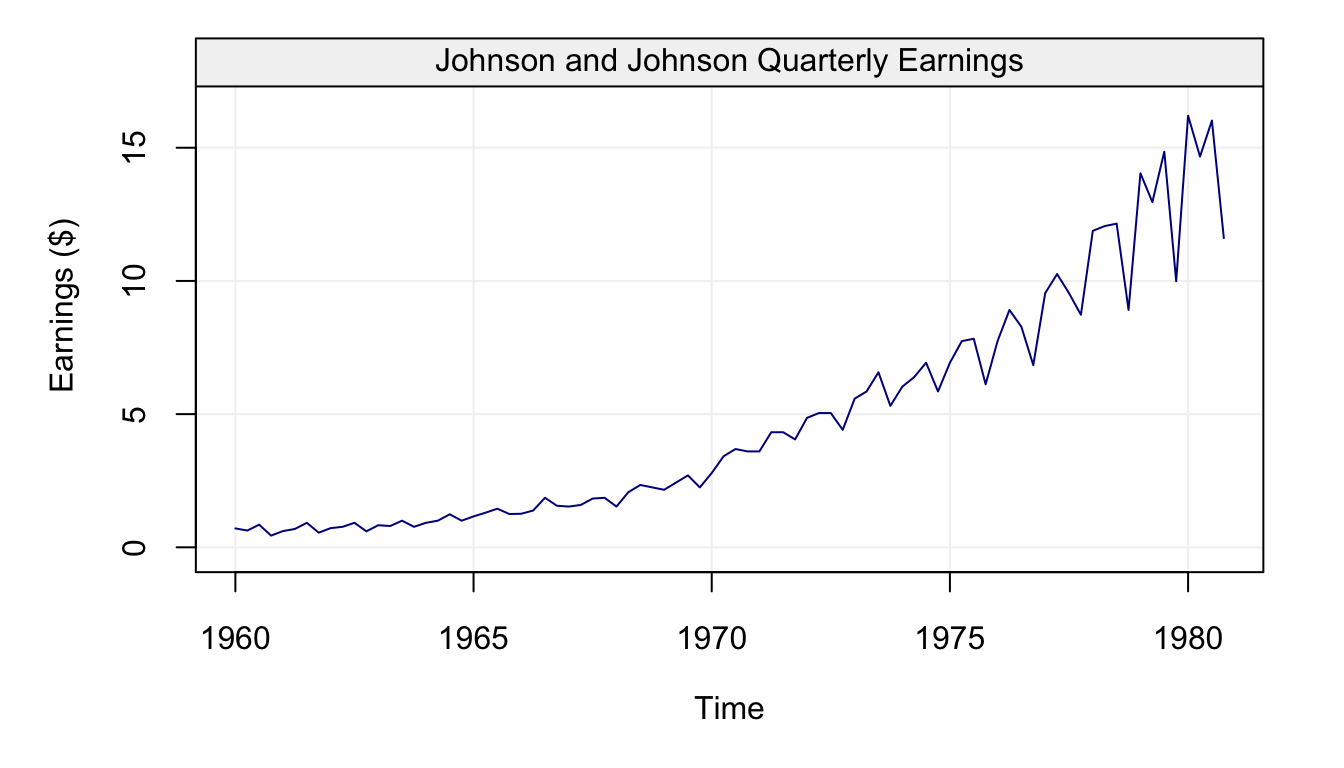
\includegraphics{tts_files/figure-latex/example_JJ-1.pdf}

One trait that the graph makes evident is that the data contains a
non-linear increasing trend as well as a yearly seasonal component. In
addition, one can note that the \emph{variability} of the data seems to
increase with time. Being able to make such observations provides
important information to select suitable models for the data.

Moreover, when observing ``raw'' time series data it is also interesting
to evaluate if some of the following phenomena occur:

\begin{enumerate}
\def\labelenumi{\arabic{enumi}.}
\tightlist
\item
  \textbf{Change in Mean:} Does the mean of the process shift over time?
\item
  \textbf{Change in Variance:} Does the variance of the process evolve
  with time?
\item
  \textbf{Change in State:} Does the time series appear to change
  between ``states'' having distinct statistical properties?
\item
  \textbf{Outliers} Does the time series contain some ``extreme''
  observations? (Note that this is typically difficult to assess
  visually.)
\end{enumerate}

\BeginKnitrBlock{example}
\protect\hypertarget{exm:earthquake}{}{\label{exm:earthquake} }In the figure
below, we present an example of displacement recorded during an
earthquake as well as an explosion.
\EndKnitrBlock{example}

\begin{Shaded}
\begin{Highlighting}[]
\CommentTok{# TO DO!}
\end{Highlighting}
\end{Shaded}

From the graph, it can be observed that the statistical properties of
the time series appear to change over time. For instance, the variance
of the time series shifts at around \(t = 1150\) for both series. The
shift in variance also opens ``windows'' where there appear to be
distinct states. In the case of the explosion data, this is particularly
relevant around \(t = 50, \cdots, 250\) and then again from
\(t = 1200, \cdots, 1500\). Even within these windows, there are
``spikes'' that could be considered as outliers most notably around
\(t = 1200\) in the explosion series.

Extreme observations or outliers are commonly observed in real time
series data, this is illustrated in the following example.

\BeginKnitrBlock{example}
\protect\hypertarget{exm:percipitation}{}{\label{exm:percipitation} }We
consider here a data set coming from the domain of hydrology. The data
concerns monthly precipitation (in mm) over a certain period of time
(1907 to 1972) and is interesting for scientists in order to study water
cycles. The data are presented in the graph below:
\EndKnitrBlock{example}

\begin{Shaded}
\begin{Highlighting}[]
\CommentTok{# Load hydro dataset}
\KeywordTok{data}\NormalTok{(}\StringTok{"hydro"}\NormalTok{)}

\CommentTok{# Simulate based on data}
\NormalTok{hydro =}\StringTok{ }\KeywordTok{gts}\NormalTok{(}\KeywordTok{as.vector}\NormalTok{(hydro), }\DataTypeTok{start =} \DecValTok{1907}\NormalTok{, }\DataTypeTok{freq =} \DecValTok{12}\NormalTok{, }\DataTypeTok{unit_ts =} \StringTok{"in."}\NormalTok{, }
            \DataTypeTok{name_ts =} \StringTok{"Precipitation"}\NormalTok{, }\DataTypeTok{data_name =} \StringTok{"Hydrology data"}\NormalTok{)}

\CommentTok{# Plot hydro }
\KeywordTok{plot}\NormalTok{(hydro)}
\end{Highlighting}
\end{Shaded}

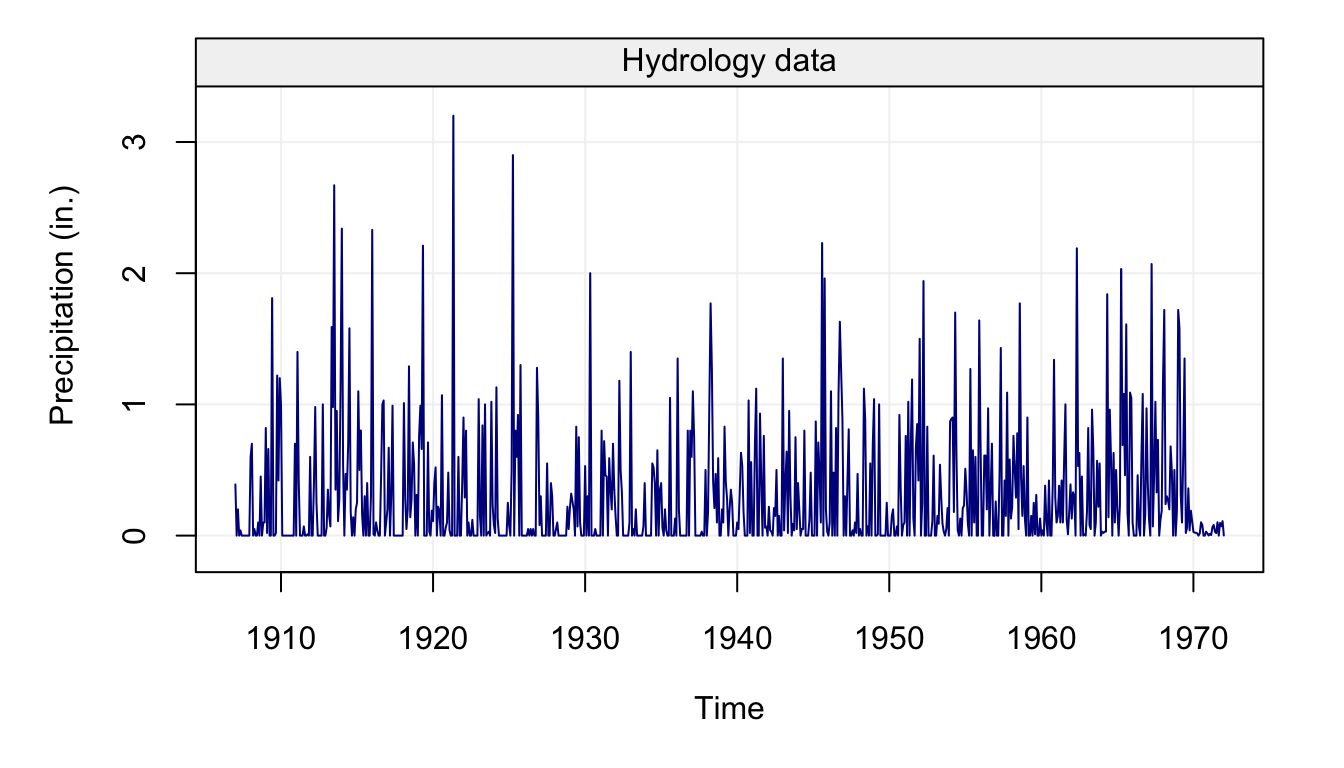
\includegraphics{tts_files/figure-latex/example_hydro-1.pdf}

Next, we consider an example coming from high-frequency finance to
illustrate the limitations our current framework.

\BeginKnitrBlock{example}
\protect\hypertarget{exm:stocks-starbucks}{}{\label{exm:stocks-starbucks}
}The figure below presents the returns or price innovations (i.e.~the
changes in price from one observation to the next) for Starbuck's stock
on July 1, 2011 for about 150 seconds (left panel) and about 400 minutes
(right panel).
\EndKnitrBlock{example}

\begin{Shaded}
\begin{Highlighting}[]
\CommentTok{# TO DO add Duke's code here!}
\end{Highlighting}
\end{Shaded}

It can be observed on the left panel that observations are not equally
spaced. Indeed, in high-frequency data the intervals between two points
are typically not constant and are, even worse, random variables. This
implies that the time when a new observation will be available is in
general unknown. On the right panel, one can observe that the
variability of the data seems to change during the course of the trading
day. Such a phenomenon is well known in the finance community since a
lot of variation occurs at the start (and the end) of the day while the
middle of the day is associated with small changes. Moreover, clear
extreme observations can also be noted in this graph at around 11:00.

Finally, let us consider the limitations of a direct graphical
representation of a time series when the sample size is large. Indeed,
due to visual limitations, a direct plotting of the data will probably
result in an uninformative aggregation of points between which it is
unable to distinguish anything. This is illustrated in the following
example.

\BeginKnitrBlock{example}
\protect\hypertarget{exm:large-imu}{}{\label{exm:large-imu} }We consider
here the data coming from the calibration procedure of an Inertial
Measurement Unit (IMU) which, in general terms, is used to enhance
navigation precision or reconstruct three dimensional movements (see
e.g. \href{https://www.youtube.com/watch?v=htoBvSq8jLA}{link}). These
sensors are used in a very wide range of applications such as robotics,
virtual reality, vehicle stability control, human and animal motion
capture and so forth (see e.g.
\href{https://www.youtube.com/watch?v=g4tgtPA54_Y}{link}). The signals
coming from these instruments are measured at high frequencies over a
long time and are often characterized by linear trends and numerous
underlying stochastic processes.
\EndKnitrBlock{example}

The code below retrieves some data from an IMU and plots it directly:

\begin{Shaded}
\begin{Highlighting}[]
\CommentTok{# Load IMU data}
\KeywordTok{data}\NormalTok{(imu6, }\DataTypeTok{package =} \StringTok{"imudata"}\NormalTok{)}

\CommentTok{# Construct gst object}
\NormalTok{Xt =}\StringTok{ }\KeywordTok{gts}\NormalTok{(imu6[,}\DecValTok{1}\NormalTok{], }\DataTypeTok{data_name =} \StringTok{"Gyroscope data"}\NormalTok{, }\DataTypeTok{unit_time =} \StringTok{"hour"}\NormalTok{, }
         \DataTypeTok{freq =} \DecValTok{100}\OperatorTok{*}\DecValTok{60}\OperatorTok{*}\DecValTok{60}\NormalTok{, }\DataTypeTok{name_ts =} \StringTok{"Angular rate"}\NormalTok{, }
         \DataTypeTok{unit_ts =} \KeywordTok{bquote}\NormalTok{(rad}\OperatorTok{^}\DecValTok{2}\OperatorTok{/}\NormalTok{s}\OperatorTok{^}\DecValTok{2}\NormalTok{))}

\CommentTok{# Plot time series}
\KeywordTok{plot}\NormalTok{(Xt)}
\end{Highlighting}
\end{Shaded}

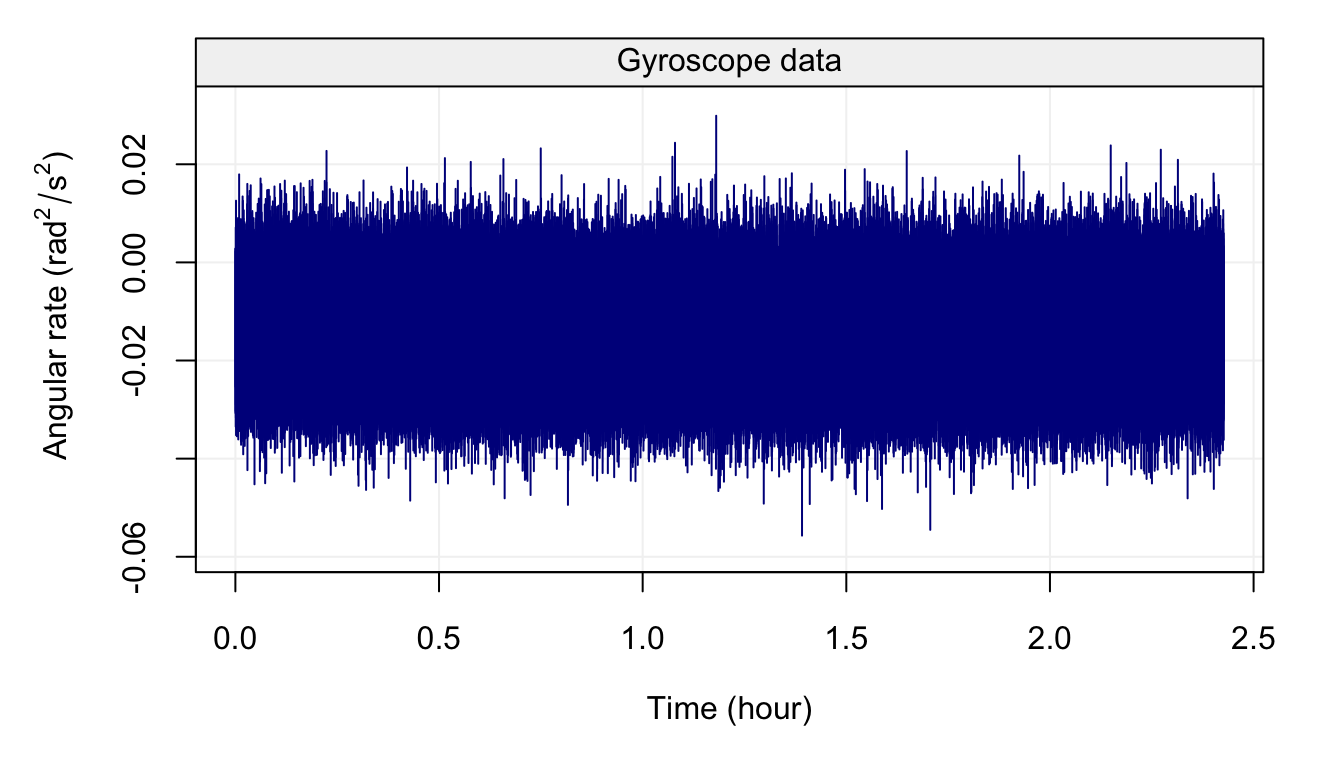
\includegraphics{tts_files/figure-latex/example_IMU-1.png}

Although a linear trend and other processes are present in this signal
(time series), it is practically impossible to understand or guess
anything from the plot.

\hypertarget{basicmodels}{%
\section{Basic Time Series Models}\label{basicmodels}}

In this section, we introduce some simple time series models. Before
doing so it is useful to define \(\Omega_t\) as all the information
avaiable up to time \(t-1\), i.e.

\[\Omega_t = \left(X_{t-1}, X_{t-2}, ..., X_0 \right).\]

As we will see this compact notation is quite useful.

\hypertarget{wn}{%
\subsection{White noise processes}\label{wn}}

The building block for most time series models is the Gaussian white
noise process, which can be defined as

\[{W_t}\mathop \sim \limits^{iid} N\left( {0,\sigma _w^2} \right).\]

This definition implies that:

\begin{enumerate}
\def\labelenumi{\arabic{enumi}.}
\tightlist
\item
  \(\mathbb{E}[W_t | \Omega_t] = 0\) for all \(t\),
\item
  \(\text{cov}\left(W_t, W_{t-h} \right) = \boldsymbol{1}_{h = 0} \; \sigma^2\)
  for all \(t, h\).
\end{enumerate}

Therefore, in this process there is an absence of temporal (or serial)
dependence and is homoskedastic (i.e.~it has a constant variance). White
noise can be generalized into two sorts of processes: \emph{weak} and
\emph{strong}. The process \((W_t)\) is a weak white noise if

\begin{enumerate}
\def\labelenumi{\arabic{enumi}.}
\tightlist
\item
  \(\mathbb{E}[W_t] = 0\) for all \(t\),
\item
  \(\text{var}\left(W_t\right) = \sigma^2\) for all \(t\),
\item
  \(\text{cov} \left(W_t, W_{t-h}\right) = 0\), for all \(t\), and for
  all \(h \neq 0\).
\end{enumerate}

Note that this definition does not imply that \(W_t\) and \(W_{t-h}\)
are independent (for \(h \neq 0\)) but simply uncorrelated. However, the
notion of independence is used to define a \emph{strong} white noise as

\begin{enumerate}
\def\labelenumi{\arabic{enumi}.}
\tightlist
\item
  \(\mathbb{E}[W_t] = 0\) and \(\text{var}(W_t) = \sigma^2 < \infty\),
  for all \(t\),
\item
  \(F(W_t) = F(W_{t-h})\), for all \(t,h\) (where \(F(W_t)\) denotes the
  distribution of \(W_t\)),
\item
  \(W_t\) and \(W_{t-h}\) are independent for all \(t\) and for all
  \(h \neq 0\).
\end{enumerate}

It is clear from these definitions that if a process is a strong white
noise it is also a weak white noise. However, the converse is not true
as shown in the following example:

\BeginKnitrBlock{example}
\protect\hypertarget{exm:weaknotstrong}{}{\label{exm:weaknotstrong} } Let
\(Y_t \mathop \sim F_{t+2}\), where \(F_{t+2}\) denotes a Student
distribution with \(t+2\) degrees of freedom. Assuming the sequence
\((Y_1, \ldots, Y_n)\) to be independent, we let
\(X_t = \sqrt{\frac{t}{t+2}} Y_t\). Then, the process \((X_t)\) is
obviously not a strong white noise as the distribution of \(X_t\)
changes with \(t\). However, this process is a weak white noise since we
have:

\begin{itemize}
\tightlist
\item
  \(\mathbb{E}[X_t] = \sqrt{\frac{t}{t+2}} \mathbb{E}[Y_t] = 0\) for all
  \(t\).
\item
  \(\text{var}(X_t) = \frac{t}{t+2} \text{var}(Y_t) = \frac{t}{t+2} \frac{t+2}{t} = 1\)
  for all \(t\).
\item
  \(\text{cov}(X_t, X_{t+h}) = 0\) (by independence), for all \(t\), and
  for all \(h \neq 0\).
\end{itemize}
\EndKnitrBlock{example}

The code below presents an example of how to simulate a Gaussian white
noise process.

\begin{Shaded}
\begin{Highlighting}[]
\NormalTok{n =}\StringTok{ }\DecValTok{1000}                               \CommentTok{# process length}
\NormalTok{sigma2 =}\StringTok{ }\DecValTok{1}                             \CommentTok{# process variance}
\NormalTok{Xt =}\StringTok{ }\KeywordTok{gen_gts}\NormalTok{(n, }\KeywordTok{WN}\NormalTok{(}\DataTypeTok{sigma2 =}\NormalTok{ sigma2))}
\KeywordTok{plot}\NormalTok{(Xt)}
\end{Highlighting}
\end{Shaded}

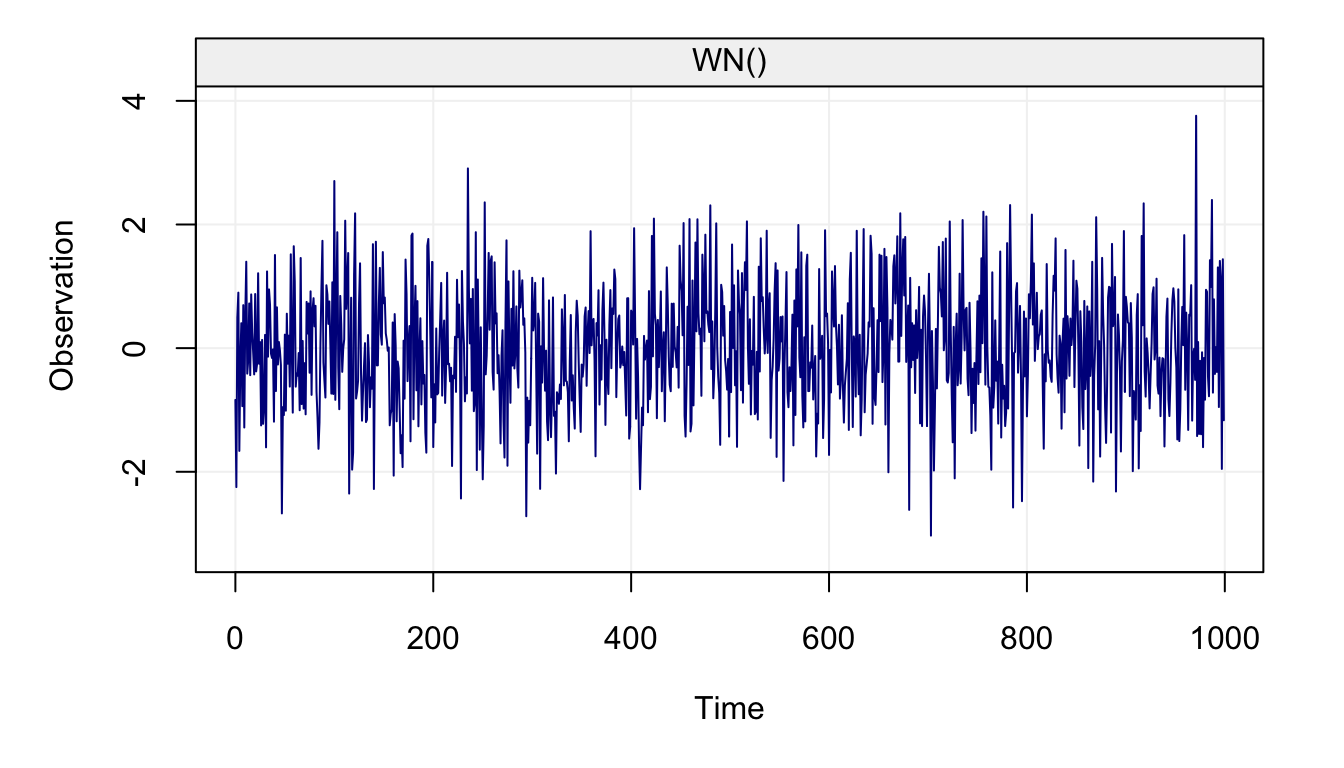
\includegraphics{tts_files/figure-latex/example_WN-1.pdf}

\hypertarget{rw}{%
\subsection{Random Walk Processes}\label{rw}}

The term \emph{random walk} was first introduced by Karl Pearson in the
early nineteen-hundreds. Regarding white noise, there exist a large
range of random walk processes. For example, one of the simplest forms
of a random walk process can be explained as follows: suppose that you
are walking on campus and your next step can either be to your left,
your right, forward or backward (each with equal probability). Two
realizations of such processes are represented below:

\begin{Shaded}
\begin{Highlighting}[]
\KeywordTok{set.seed}\NormalTok{(}\DecValTok{5}\NormalTok{)}
\KeywordTok{RW2dimension}\NormalTok{(}\DataTypeTok{steps =} \DecValTok{10}\OperatorTok{^}\DecValTok{2}\NormalTok{)}
\end{Highlighting}
\end{Shaded}

\begin{center}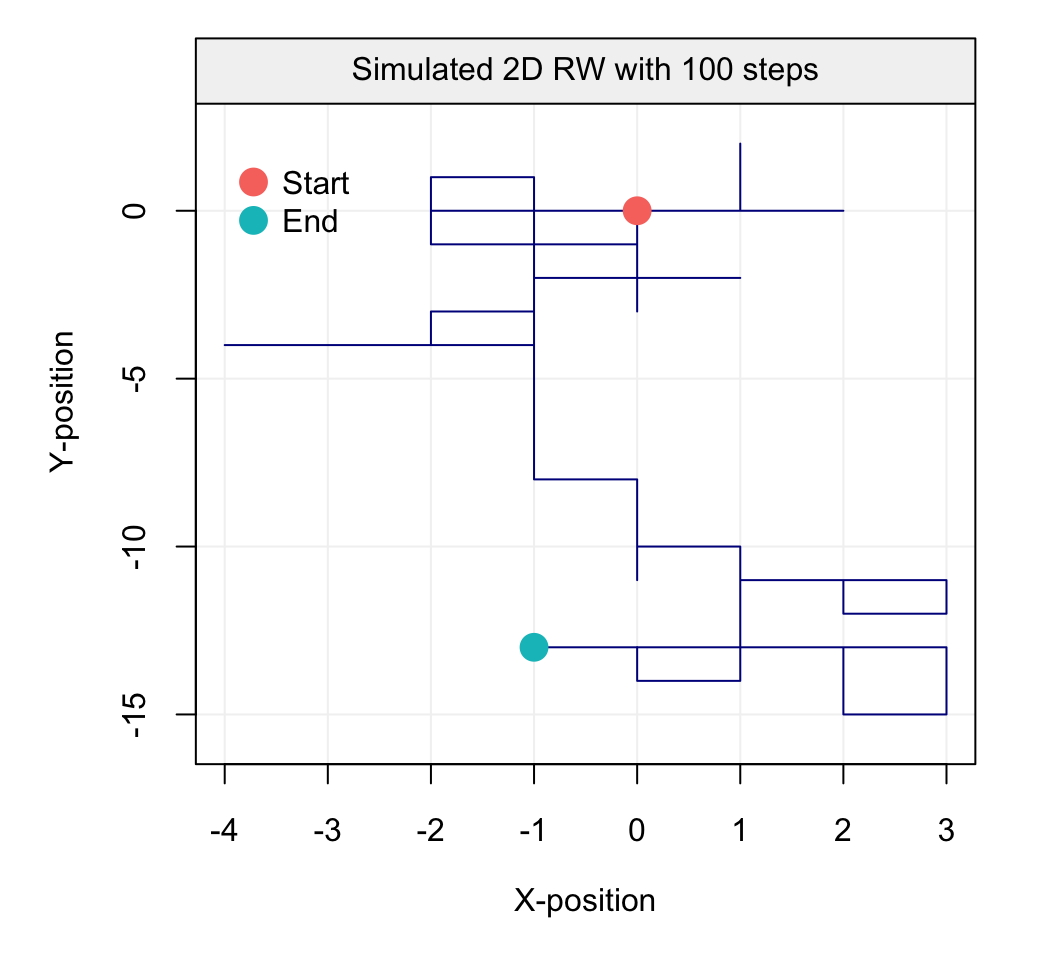
\includegraphics{tts_files/figure-latex/RW2d-1} \end{center}

\begin{Shaded}
\begin{Highlighting}[]
\KeywordTok{RW2dimension}\NormalTok{(}\DataTypeTok{steps =} \DecValTok{10}\OperatorTok{^}\DecValTok{4}\NormalTok{)}
\end{Highlighting}
\end{Shaded}

\begin{center}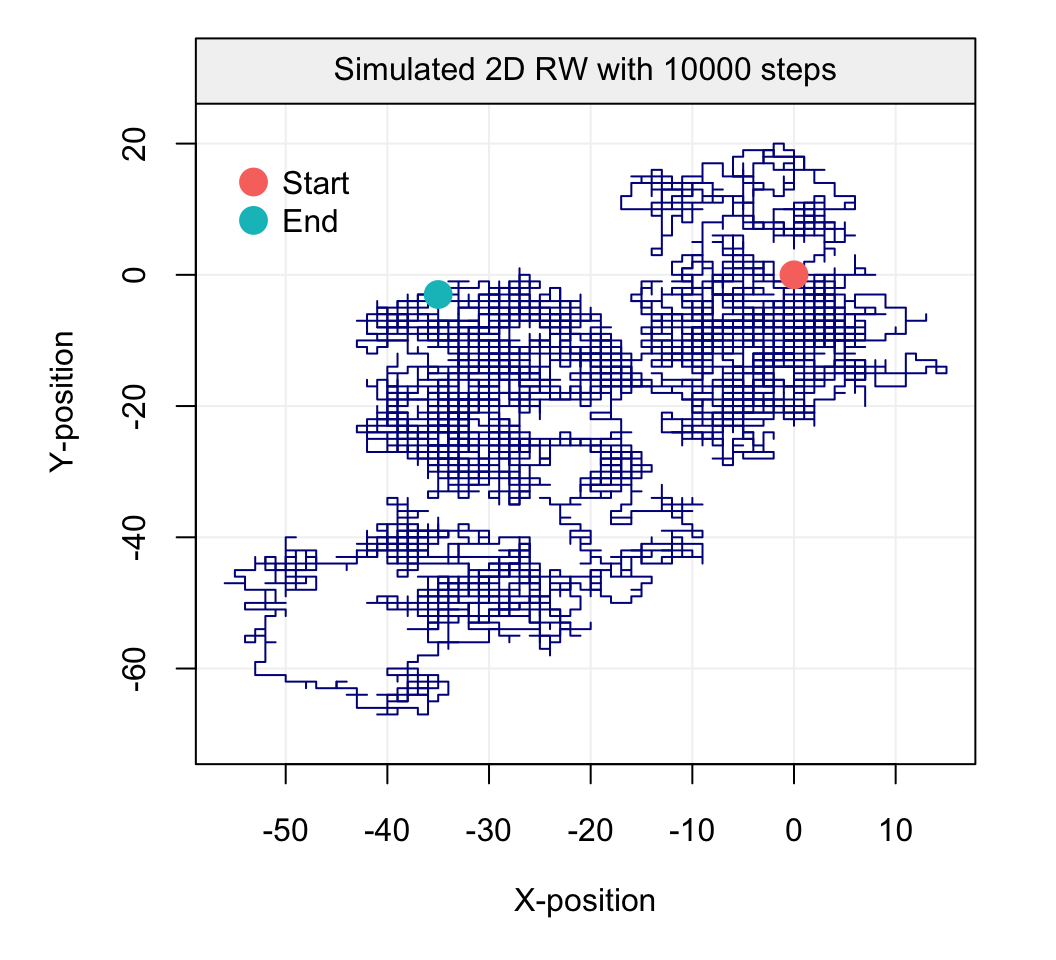
\includegraphics{tts_files/figure-latex/RW2d-2} \end{center}

Such processes inspired Karl Pearson's famous quote that

\begin{quote}
``\emph{the most likely place to find a drunken walker is somewhere near
his starting point.}''
\end{quote}

Empirical evidence of this phenomenon is not too hard to find on a
Friday night. In this text, we only consider one very specific form of
random walk, namely the Gaussian random walk which can be defined as:

\[X_t = X_{t-1} + W_t,\]

where \(W_t\) is a Gaussian white noise process with initial condition
\(X_0 = c\). (Typically \(c = 0\).) This process can be expressed
differently by \emph{backsubstitution} as follows:

\[\begin{aligned}
  {X_t} &= {X_{t - 1}} + {W_t} \\
   &= \left( {{X_{t - 2}} + {W_{t - 1}}} \right) + {W_t} \\
   &= \vdots \\
  {X_t} &= \sum\limits_{i = 1}^t {{W_i}} + X_0 =  \sum\limits_{i = 1}^t {{W_i}} + c \\ 
\end{aligned} \]

The code below presents an example of how to simulate a such process.

\begin{Shaded}
\begin{Highlighting}[]
\NormalTok{n =}\StringTok{ }\DecValTok{1000}                               \CommentTok{# process length}
\NormalTok{gamma2 =}\StringTok{ }\DecValTok{1}                             \CommentTok{# innovation variance}
\NormalTok{Xt =}\StringTok{ }\KeywordTok{gen_gts}\NormalTok{(n, }\KeywordTok{RW}\NormalTok{(}\DataTypeTok{gamma2 =}\NormalTok{ gamma2))}
\KeywordTok{plot}\NormalTok{(Xt)}
\end{Highlighting}
\end{Shaded}

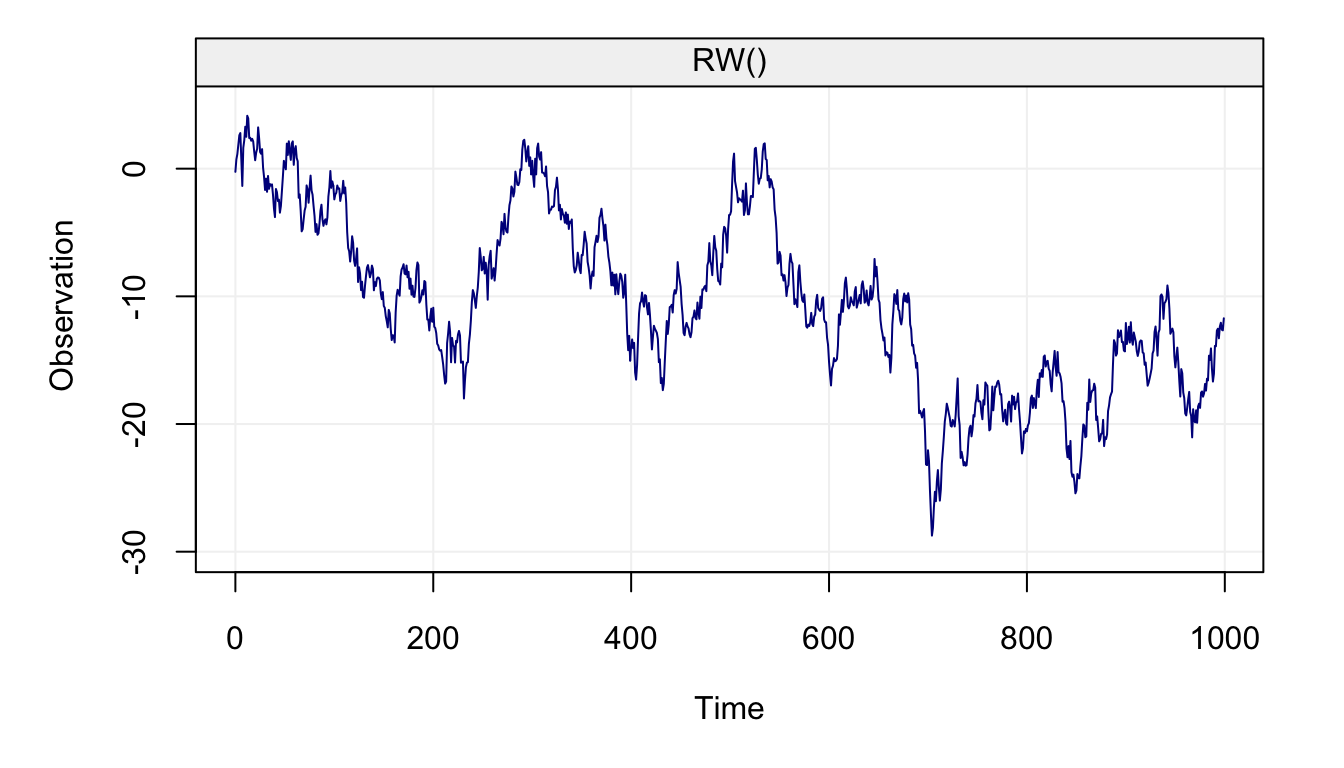
\includegraphics{tts_files/figure-latex/example_RW-1.pdf}

\hypertarget{ar1}{%
\subsection{Autoregressive Process of Order 1}\label{ar1}}

An autoregressive process of order 1 or AR(1) is a generalization of
both the white noise and random walk processes which are both themselves
special cases of an AR(1). A (Gaussian) AR(1) process can be defined as

\[{X_t} = {\phi}{X_{t - 1}} + {W_t},\]

where \(W_t\) is a Gaussian white noise. Clearly, an AR(1) with
\(\phi = 0\) is a Gaussian white noise and when \(\phi = 1\) the process
becomes a random walk.

\BeginKnitrBlock{remark}
\iffalse{} {Remark. } \fi{}We generally assume that an AR(1), as well as
other time series models, have zero mean. The reason for this assumption
is only to simplfy the notation but it is easy to consider an AR(1)
process around an arbitrary mean \(\mu\), i.e.

\[\left(X_t - \mu\right) = \phi \left(X_{t-1} - \mu \right) + W_t,\]

which is of course equivalent to

\[X_t = \left(1 - \phi \right) \mu + \phi X_{t-1} + W_t.\]

Thus, we will generally only work with zero mean processes since adding
means is simple.
\EndKnitrBlock{remark}

\BeginKnitrBlock{remark}
\iffalse{} {Remark. } \fi{}An AR(1) is in fact a linear combination of
past realisations of the white noise \(W_t\) process. Indeed, we have

\[\begin{aligned}
 {X_t} &= {\phi_t}{X_{t - 1}} + {W_t} 
   = {\phi}\left( {{\phi}{X_{t - 2}} + {W_{t - 1}}} \right) + {W_t} \\
   &= \phi^2{X_{t - 2}} + {\phi}{W_{t - 1}} + {W_t} 
   = {\phi^t}{X_0} + \sum\limits_{i = 0}^{t - 1} {\phi^i{W_{t - i}}}.
\end{aligned}\]

Under the assumption of infinite past (i.e. \(t \in \mathbb{Z}\)) and
\(|\phi| < 1\), we obtain

\[X_t = \sum\limits_{i = 0}^{\infty} {\phi^i {W_{t - i}}},\]

since \(\operatorname{lim}_{i \to \infty} \; {\phi^i}{X_{t-i}} = 0\).
\EndKnitrBlock{remark}

The code below presents an example of how an AR(1) can be simulated.

\begin{Shaded}
\begin{Highlighting}[]
\NormalTok{n =}\StringTok{ }\DecValTok{1000}                              \CommentTok{# process length}
\NormalTok{phi =}\StringTok{ }\FloatTok{0.5}                             \CommentTok{# phi parameter}
\NormalTok{sigma2 =}\StringTok{ }\DecValTok{1}                            \CommentTok{# innovation variance}
\NormalTok{Xt =}\StringTok{ }\KeywordTok{gen_gts}\NormalTok{(n, }\KeywordTok{AR1}\NormalTok{(}\DataTypeTok{phi =}\NormalTok{ phi, }\DataTypeTok{sigma2 =}\NormalTok{ sigma2))}
\KeywordTok{plot}\NormalTok{(Xt)}
\end{Highlighting}
\end{Shaded}

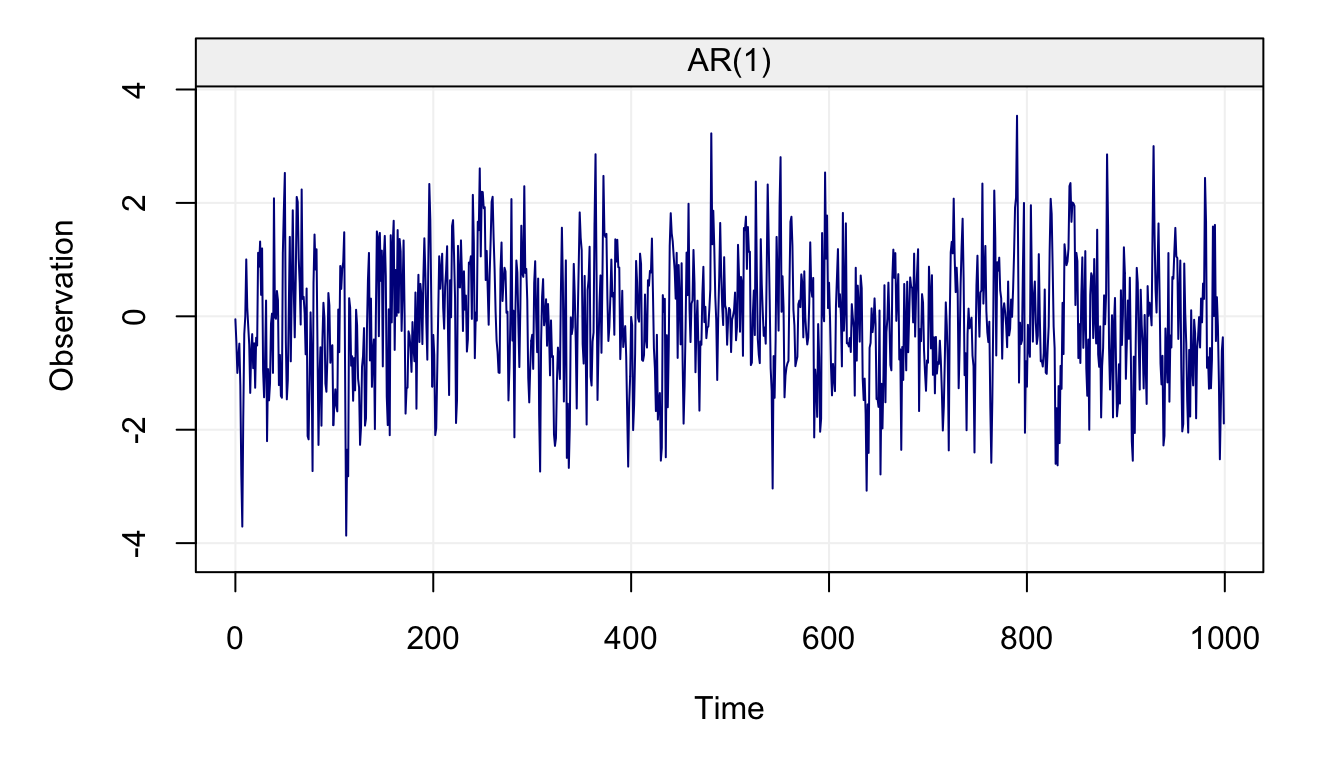
\includegraphics{tts_files/figure-latex/example_AR1-1.pdf}

\hypertarget{ma1}{%
\subsection{Moving Average Process of Order 1}\label{ma1}}

As we have seen in the previous example, an AR(1) can be expressed as a
linear combination of all past observations of \((W_t)\) while the next
process, called a moving average process of order 1 or MA(1), is (in
some sense) a ``truncated'' version of an AR(1). It is defined as

\begin{equation} 
  X_t = \theta W_{t-1} + W_t,
\end{equation}

where (again) \(W_t\) denotes a Gaussian white noise process. An example
on how to generate an MA(1) is given below:

\begin{Shaded}
\begin{Highlighting}[]
\NormalTok{n =}\StringTok{ }\DecValTok{1000}                              \CommentTok{# process length}
\NormalTok{sigma2 =}\StringTok{ }\DecValTok{1}                            \CommentTok{# innovation variance}
\NormalTok{theta =}\StringTok{ }\FloatTok{0.5}                           \CommentTok{# theta parameter}
\NormalTok{Xt =}\StringTok{ }\KeywordTok{gen_gts}\NormalTok{(n, }\KeywordTok{MA1}\NormalTok{(}\DataTypeTok{theta =}\NormalTok{ theta, }\DataTypeTok{sigma2 =}\NormalTok{ sigma2))}
\KeywordTok{plot}\NormalTok{(Xt)}
\end{Highlighting}
\end{Shaded}

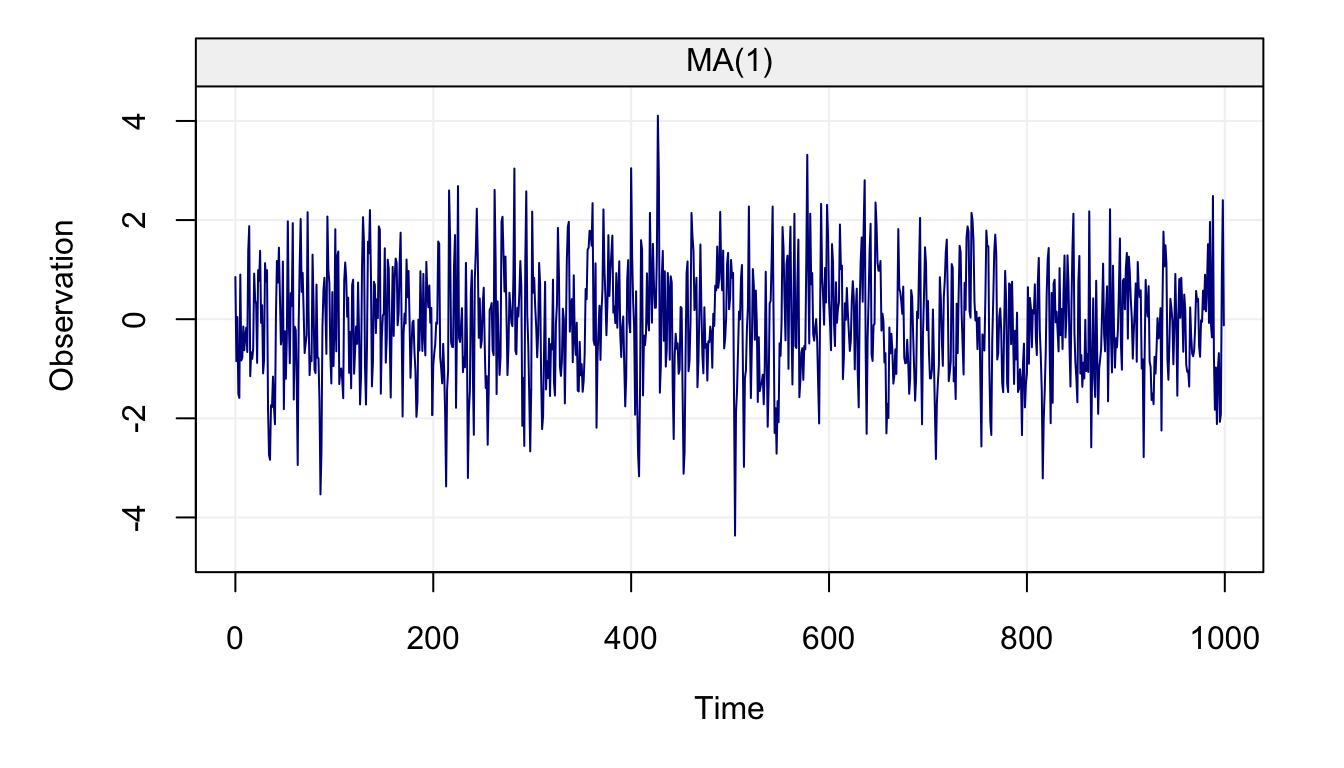
\includegraphics{tts_files/figure-latex/example_MA1-1.pdf}

\hypertarget{drift}{%
\subsection{Linear Drift}\label{drift}}

A linear drift is a very simple deterministic time series model which
can be expressed as

\[X_t = X_{t-1} + \omega, \]

where \(\omega\) is a constant and with the initial condition
\(X_0 = c\), where \(c\) is an arbitrary constant (typically zero). This
process can be expressed in a more familiar form as follows:

\[
  {X_t} = {X_{t - 1}} + \omega 
   = \left( {{X_{t - 2}} + \omega} \right) + \omega 
   = t{\omega} + c  \]

Therefore, a (linear) drift corresponds to a simple linear model with
slope \(\omega\) and intercept \(c\).

A drift can simply be generated using the code below:

\begin{Shaded}
\begin{Highlighting}[]
\NormalTok{n =}\StringTok{ }\DecValTok{100}                               \CommentTok{# process length}
\NormalTok{omega =}\StringTok{ }\FloatTok{0.5}                           \CommentTok{# slope parameter}
\NormalTok{Xt =}\StringTok{ }\KeywordTok{gen_gts}\NormalTok{(n, }\KeywordTok{DR}\NormalTok{(}\DataTypeTok{omega =}\NormalTok{ omega))}
\KeywordTok{plot}\NormalTok{(Xt)}
\end{Highlighting}
\end{Shaded}

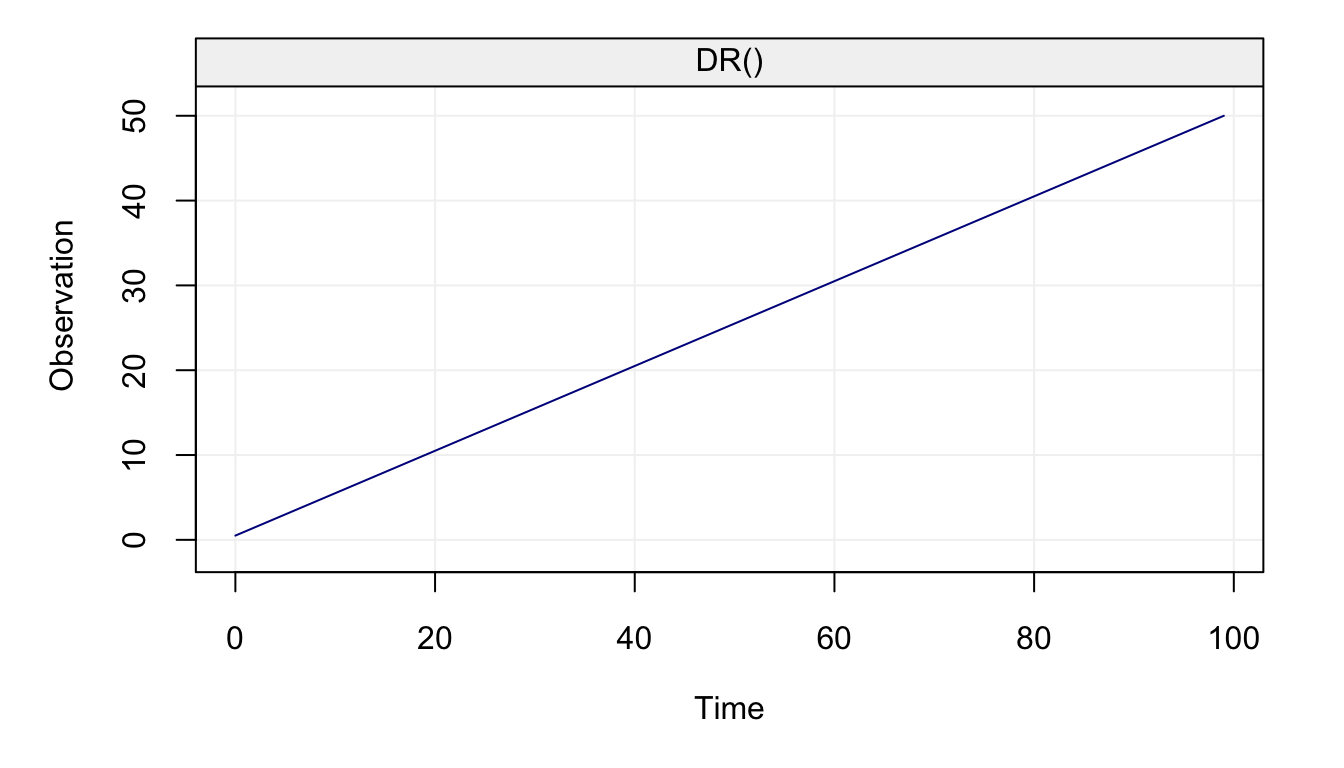
\includegraphics{tts_files/figure-latex/example_Drift-1.pdf}

\hypertarget{lts}{%
\section{Composite Stochastic Processes}\label{lts}}

A composite stochastic process can be defined as the sum of underlying
(or latent) stochastic processes. In this text, we will use the term
\emph{latent time series} as a synomym for composite stochastic
processes. A simple example of such a process is given by

\[\begin{aligned}
Y_t &= Y_{t-1} + W_t + \delta\\
X_t &= Y_t + Z_t,
\end{aligned}\]

where \(W_t\) and \(Z_t\) are two independent Gaussian white noise
processes. This model is often used as a first tool to approximate the
number of individuals in the context ecological population dynamics. For
example, suppose we want to study the population of Chamois in the Swiss
Alps. Let \(Y_t\) denote the ``true'' number of individuals in this
population at time \(t\). It is reasonable that \(Y_t\) is
(approximately) the population at the previous time \(t-1\) (e.g the
previous year) plus a random variation and a drift. This random
variation is due to the natural randomness in ecological population
dynamics and reflects changes such as the number of predators, the
abundance of food, or weather conditions. On the other hand, ecological
\emph{drift} is often of particular interest for ecologists as it can be
used to determine the ``long'' term trends of the population (e.g.~if
the population is increasing, decreasing, or stable). Of course, \(Y_t\)
(the number of individauls) is typically unknown and we observe a noisy
version of it, denoted as \(X_t\). This process corresponds to the true
population plus a measurement error since some individuals may not be
observed while others may have been counted several times.
Interestingly, this process can clearly be expressed as a \emph{latent
time series model} (or composite stochastic process) as follows:

\[\begin{aligned}
R_t &= R_{t-1} + W_t \\
S_t &= \delta t \\
X_t &= R_t + S_t + Z_t,
\end{aligned}\]

where \(R_t\), \(S_t\) and \(Z_t\) denote, respectively, a random walk,
a drift, and a white noise. The code below can be used to simulate such
data:

\begin{Shaded}
\begin{Highlighting}[]
\NormalTok{n =}\StringTok{ }\DecValTok{1000}                                \CommentTok{# process length}
\NormalTok{delta =}\StringTok{ }\FloatTok{0.005}                           \CommentTok{# delta parameter (drift)}
\NormalTok{sigma2 =}\StringTok{ }\DecValTok{10}                             \CommentTok{# variance parameter (white noise)}
\NormalTok{gamma2 =}\StringTok{ }\FloatTok{0.1}                            \CommentTok{# innovation variance (random walk)}
\NormalTok{model =}\StringTok{ }\KeywordTok{WN}\NormalTok{(}\DataTypeTok{sigma2 =}\NormalTok{ sigma2) }\OperatorTok{+}\StringTok{ }\KeywordTok{RW}\NormalTok{(}\DataTypeTok{gamma2 =}\NormalTok{ gamma2) }\OperatorTok{+}\StringTok{ }\KeywordTok{DR}\NormalTok{(}\DataTypeTok{omega =}\NormalTok{ delta)}
\NormalTok{Xt =}\StringTok{ }\KeywordTok{gen_lts}\NormalTok{(n, model)}
\KeywordTok{plot}\NormalTok{(Xt)}
\end{Highlighting}
\end{Shaded}

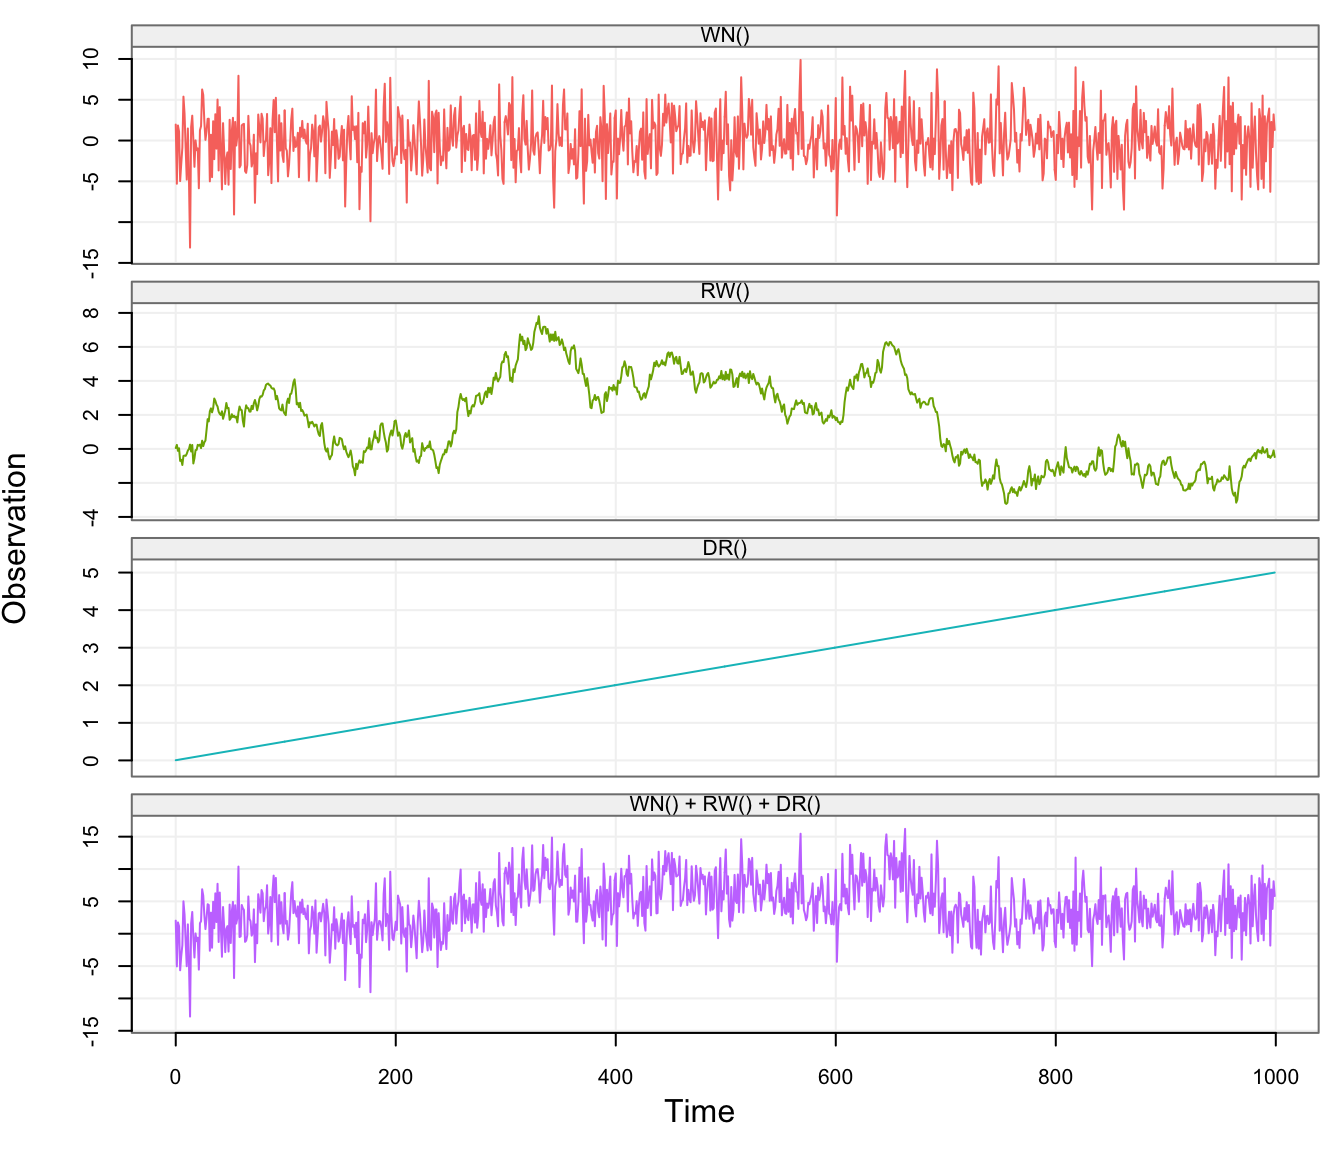
\includegraphics{tts_files/figure-latex/example_composite-1.pdf}

In the above graph, the first three plots represent the latent
(unobserved) processes (i.e.~white noise, random walk, and drift) and
the last one represents the sum of the three (i.e. \((X_t)\)).

Let us consider a real example where these latent processes are useful
to describe (and predict) the behavior of economic variables such as
Personal Saving Rates (PSR). A process that is used for these settings
is the ``random-walk-plus-noise'' model, meaning that the data can be
explained by a random walk process in addition to which we observe some
other process (e.g. a white noise model, an autoregressive model such as
an AR(1), etc.). The PSR taken from the Federal Reserve of St.~Louis
from January 1, 1959, to May 1, 2015, is presented in the following
plot:

\begin{Shaded}
\begin{Highlighting}[]
\CommentTok{# Load savingrt dataset}
\KeywordTok{data}\NormalTok{(}\StringTok{"savingrt"}\NormalTok{)}
\CommentTok{# Simulate based on data}
\NormalTok{savingrt =}\StringTok{ }\KeywordTok{gts}\NormalTok{(}\KeywordTok{as.vector}\NormalTok{(savingrt), }\DataTypeTok{start =} \DecValTok{1959}\NormalTok{, }\DataTypeTok{freq =} \DecValTok{12}\NormalTok{, }\DataTypeTok{unit_ts =} \StringTok{"%"}\NormalTok{, }
            \DataTypeTok{name_ts =} \StringTok{"Saving Rates"}\NormalTok{, }\DataTypeTok{data_name =} \StringTok{"US Personal Saving Rates"}\NormalTok{)}
\CommentTok{# Plot savingrt simulation}
\KeywordTok{plot}\NormalTok{(savingrt)}
\end{Highlighting}
\end{Shaded}

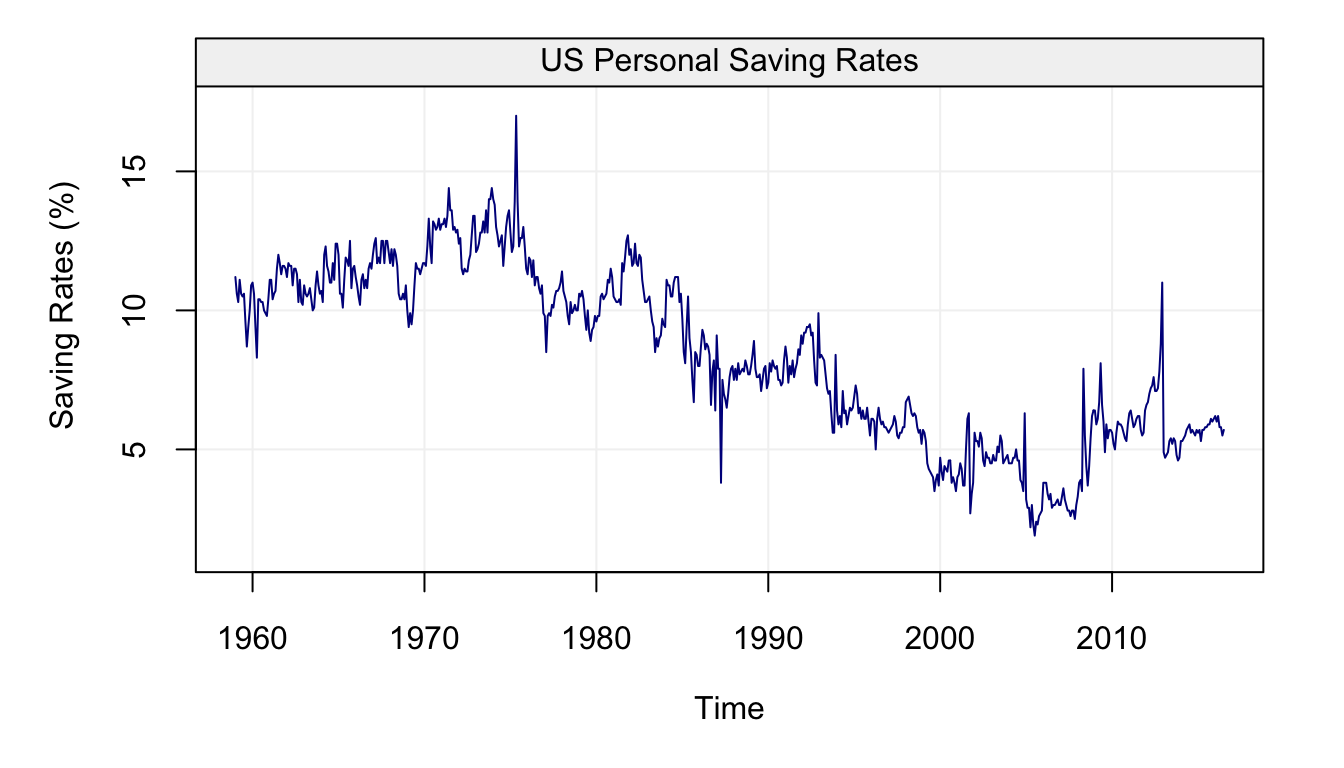
\includegraphics{tts_files/figure-latex/example_PSR-1.pdf}

It can be observed that the mean of this process seems to vary over
time, suggesting that a random walk can indeed be considered as a
possible model to explain this data. In addition, aside from some
``spikes'' and occasional sudden changes, the observations appear to
gradually change from one time point to the other, suggesting that some
other form of dependence between them could exist.

\hypertarget{autocorrelation-and-stationarity}{%
\chapter{Autocorrelation and
Stationarity}\label{autocorrelation-and-stationarity}}

\begin{quote}
``\emph{One of the first things taught in introductory statistics
textbooks is that correlation is not causation. It is also one of the
first things forgotten.}'' -- Thomas Sowell
\end{quote}

In this chapter we will discuss and formalize how knowledge about
\(X_{t-1}\) (or more generally about all the information from the past,
\(\Omega_t\)) can provide us with some information about the properties
of \(X_t\). In particular, we will consider the correlation (or
covariance) of \(X_t\) at different times such as
\(\text{corr} \left(X_t, X_{t+h}\right)\). This ``form'' of correlation
(covariance) is called the \emph{autocorrelation}
(\emph{autocovariance}) and is a very useful tool in time series
analysis. However, if we do not assume that a time series is
characterized by a certain form of ``stability'', it would be rather
difficult to estimate \(\text{corr} \left(X_t, X_{t+h}\right)\) as this
quantity would depend on both \(t\) and \(h\) leading to more parameters
to estimate than observations available. Therefore, the concept of
\emph{stationarity} is convenient in this context as it allows (among
other things) to assume that

\[\text{corr} \left(X_t, X_{t+h}\right) = \text{corr} \left(X_{t+j}, X_{t+h+j}\right), \;\;\; \text{for all $j$},\]

implying that the autocorrelation (or autocovariance) is only a function
of the lag between observations, rather than time itself. These two
concepts (i.e. autocorrelation and stationarity) will be discussed in
this chapter. Before moving on, it is helpful to remember that
correlation (or autocorrelation) is only appropriate to measure a very
specific kind of dependence, i.e.~the linear dependence. There are many
other forms of dependence as illustrated in the bottom panels of the
graph below, which all have a (true) zero correlation:

\begin{figure}

{\centering 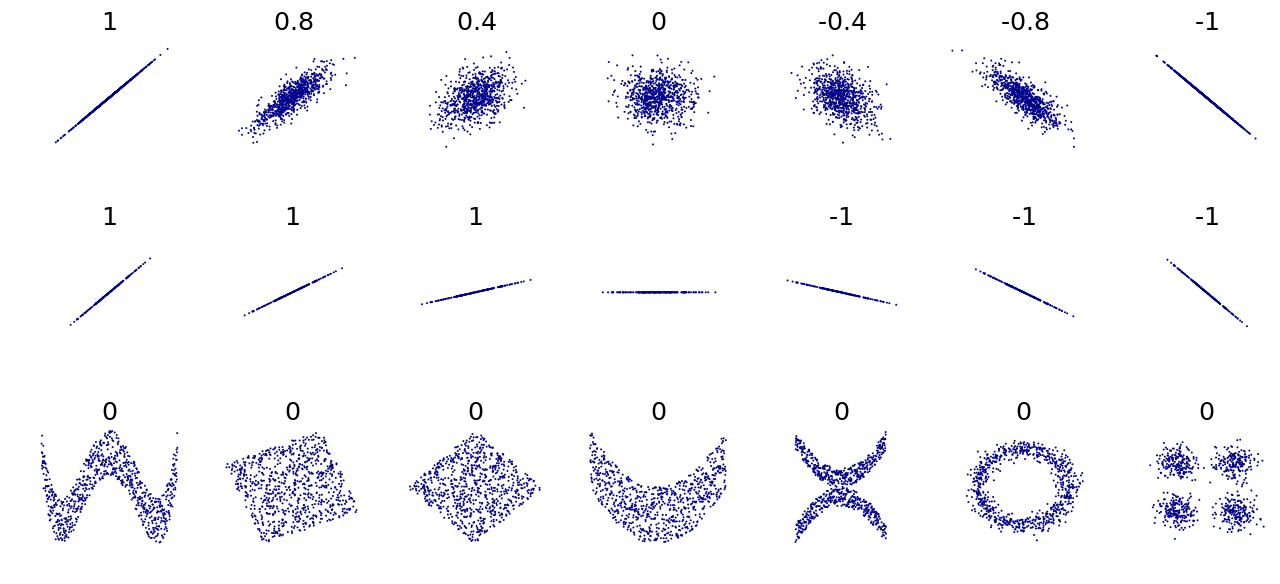
\includegraphics[width=17.78in]{images/corr_example} 

}

\caption{Different forms of dependence and their Pearson's r values}\label{fig:correxample}
\end{figure}

Several other metrics have been introduced in the literature to assess
the degree of ``dependence'' of two random variables, however this goes
beyond the material discussed in this chapter.

\hypertarget{the-autocorrelation-and-autocovariance-functions}{%
\section{The Autocorrelation and Autocovariance
Functions}\label{the-autocorrelation-and-autocovariance-functions}}

\BeginKnitrBlock{definition}
\protect\hypertarget{def:acvf}{}{\label{def:acvf} }The \emph{autocovariance
function} of a series \((X_t)\) is defined as

\[{\gamma_x}\left( {t,t+h} \right) = \text{cov} \left( {{X_t},{X_{t+h}}} \right),\]
\EndKnitrBlock{definition}

where the definition of covariance is given by:

\[
    \text{cov} \left( {{X_t},{X_{t+h}}} \right) = \mathbb{E}\left[ {{X_t}{X_{t+h}}} \right] - \mathbb{E}\left[ {{X_t}} \right]\mathbb{E}\left[ {{X_{t+h}}} \right].
    \]

Similarly, the above expectations are defined to be:

\[\begin{aligned}
     \mathbb{E}\left[ {{X_t}} \right] &= \int\limits_{ - \infty }^\infty  {x \cdot {f_t}\left( x \right)dx},  \\
     \mathbb{E}\left[ {{X_t}{X_{t+h}}} \right] &= \int\limits_{ - \infty }^\infty  {\int\limits_{ - \infty }^\infty  {{x_1}{x_2} \cdot f_{t,t+h}\left( {{x_1},{x_2}} \right)d{x_1}d{x_2}} } ,
     \end{aligned} \]

where \({f_t}\left( x \right)\) and
\(f_{t,t+h}\left( {{x_1},{x_2}} \right)\) denote, respectively, the
density of \(X_t\) and the joint density of the pair \((X_t, X_{t+h})\).
For the notation, it should be clear that \(X_t\) is assumed to be a
continous random variable. Since we generally consider stochastic
processes with constant zero mean, we often have

\[{\gamma_x}\left( {t,t+h} \right) = \mathbb{E}\left[X_t X_{t+h} \right]. \]

In addition, we normally drop the subscript referring to the time series
(i.e. \(x\) in this case) if it is clear from the context which time
series the autocovariance refers to. For example, we generally use
\({\gamma}\left( {t,t+h} \right)\) instead of
\({\gamma_x}\left( {t,t+h} \right)\). Moreover, the notation is even
further simplified when the covariance of \(X_t\) and \(X_{t+h}\) is the
same as that of \(X_{t+j}\) and \(X_{t+h+j}\) (for all \(j\)), i.e.~the
covariance depends only on the time between observations and not on the
specific time \(t\). This is an important property called
\emph{stationarity}, which will be discussed in the next section. In
this case, we simply use to following notation:
\[\gamma \left( {h} \right) = \text{cov} \left( X_t , X_{t+h} \right). \]

This notation will generally be used throughout the text and implies
certain properties (i.e.~stationarity) on the process \((X_t)\). Several
remarks can be made on the autocovariance:

\begin{enumerate}
\def\labelenumi{\arabic{enumi}.}
\tightlist
\item
  The autocovariance function is \emph{symmetric}. That is,
  \({\gamma}\left( {h} \right) = {\gamma}\left( -h \right)\) since
  \(\text{cov} \left( {{X_t},{X_{t+h}}} \right) = \text{cov} \left( X_{t+h},X_{t} \right)\).
\item
  The autocovariance function ``contains'' the variance of the process
  as \(\text{var} \left( X_{t} \right) = {\gamma}\left( 0 \right)\).
\item
  We have that \(|\gamma(h)| \leq \gamma(0)\) for all \(h\). The proof
  of this inequality is direct and follows from the Cauchy-Schwarz
  inequality, i.e. \[ \begin{aligned}
    \left(|\gamma(h)| \right)^2 &= \gamma(h)^2 = \left(\mathbb{E}\left[\left(X_t - \mathbb{E}[X_t] \right)\left(X_{t+h} - \mathbb{E}[X_{t+h}] \right)\right]\right)^2\\
    &\leq \mathbb{E}\left[\left(X_t - \mathbb{E}[X_t] \right)^2 \right] \mathbb{E}\left[\left(X_{t+h} - \mathbb{E}[X_{t+h}] \right)^2 \right] =  \gamma(0)^2. 
    \end{aligned}
    \]
\item
  Just as any covariance, \({\gamma}\left( {h} \right)\) is ``scale
  dependent'' since \({\gamma}\left( {h} \right) \in \mathbb{R}\), or
  \(-\infty \le {\gamma}\left( {h} \right) \le +\infty\). We therefore
  have:
\end{enumerate}

\begin{itemize}
\tightlist
\item
  if \(\left| {\gamma}\left( {h} \right) \right|\) is ``close'' to zero,
  then \(X_t\) and \(X_{t+h}\) are ``weakly'' (linearly) dependent;
\item
  if \(\left| {\gamma}\left( {h} \right) \right|\) is ``far'' from zero,
  then the two random variable present a ``strong'' (linear) dependence.
  However it is generally difficult to asses what ``close'' and ``far''
  from zero means in this case.
\end{itemize}

\begin{enumerate}
\def\labelenumi{\arabic{enumi}.}
\setcounter{enumi}{4}
\tightlist
\item
  \({\gamma}\left( {h} \right)=0\) does not imply that \(X_t\) and
  \(X_{t+h}\) are independent but simply \(X_t\) and \(X_{t+h}\) are
  uncorrelated. The independence is only implied by
  \({\gamma}\left( {h} \right)=0\) in the jointly Gaussian case.
\end{enumerate}

As hinted in the introduction, an important related statistic is the
correlation of \(X_t\) with \(X_{t+h}\) or \emph{autocorrelation}, which
is defined as

\[\rho \left(  h \right) = \text{corr}\left( {{X_t},{X_{t + h}}} \right) = \frac{{\text{cov}\left( {{X_t},{X_{t + h}}} \right)}}{{{\sigma _{{X_t}}}{\sigma _{{X_{t + h}}}}}} = \frac{\gamma(h) }{\gamma(0)}.\]

Similarly to \(\gamma(h)\), it is important to note that the above
notation implies that the autocorrelation function is only a function of
the lag \(h\) between observations. Thus, autocovariances and
autocorrelations are one possible way to describe the joint distribution
of a time series. Indeed, the correlation of \(X_t\) with \(X_{t+1}\) is
an obvious measure of how \emph{persistent} a time series is.

Remember that just as with any correlation:

\begin{enumerate}
\def\labelenumi{\arabic{enumi}.}
\tightlist
\item
  \(\rho \left( h \right)\) is ``scale free'' so it is much easier to
  interpret than \(\gamma(h)\).
\item
  \(|\rho \left( h \right)| \leq 1\) since
  \(|\gamma(h)| \leq \gamma(0)\).
\item
  \textbf{Causation and correlation are two very different things!}
\end{enumerate}

\hypertarget{a-fundamental-representation}{%
\subsection{A Fundamental
Representation}\label{a-fundamental-representation}}

Autocovariances and autocorrelations also turn out to be very useful
tools as they are one of the \emph{fundamental representations} of time
series. Indeed, if we consider a zero mean normally distributed process,
it is clear that its joint distribution is fully characterized by the
autocovariances \(\mathbb{E}[X_t X_{t+h}]\) (since the joint probability
density only depends of these covariances). Once we know the
autocovariances we know \emph{everything} there is to know about the
process and therefore:

\emph{if two processes have the same autocovariance function, then they
are the same process.}

\hypertarget{admissible-autocorrelation-functions}{%
\subsection{Admissible Autocorrelation
Functions}\label{admissible-autocorrelation-functions}}

Since the autocorrelation is related to a fundamental representation of
time series, it implies that one might be able to define a stochastic
process by picking a set of autocorrelation values (assuming for example
that \(\text{var}(X_t) = 1\)). However, it turns out that not every
collection of numbers, say \(\{\rho_1, \rho_2, ...\}\), can represent
the autocorrelation of a process. Indeed, two conditions are required to
ensure the validity of an autocorrelation sequence:

\begin{enumerate}
\def\labelenumi{\arabic{enumi}.}
\tightlist
\item
  \(\operatorname{max}_j \; | \rho_j| \leq 1\).
\item
  \(\text{var} \left[\sum_{j = 0}^\infty \alpha_j X_{t-j} \right] \geq 0 \;\)
  for all \(\{\alpha_0, \alpha_1, ...\}\).
\end{enumerate}

The first condition is obvious and simply reflects the fact that
\(|\rho \left( h \right)| \leq 1\) but the second is far more difficult
to verify. To further our understanding of the latter we let
\(\alpha_j = 0\) for \(j > 1\), then condition two implies that

\[\text{var} \left[ \alpha_0 X_{t} + \alpha_1 X_{t-1}  \right] = \gamma_0 \begin{bmatrix}
   \alpha_0 & \alpha_1
   \end{bmatrix}   \begin{bmatrix}
   1 & \rho_1\\
   \rho_1 & 1
   \end{bmatrix} \begin{bmatrix}
   \alpha_0 \\
   \alpha_1
   \end{bmatrix} \geq 0. \]

Thus, the matrix

\[ \boldsymbol{A}_1 = \begin{bmatrix}
  1 & \rho_1\\
  \rho_1 & 1
  \end{bmatrix} \]

must be positive semi-definite. Taking the determinant we have

\[\operatorname{det} \left(\boldsymbol{A}_1\right) = 1 - \rho_1^2 \]

implying that the condition \(|\rho_1| \leq 1\) must be respected. Now,
let \(\alpha_j = 0\) for \(j > 2\), then we must verify that:

\[\text{var} \left[ \alpha_0 X_{t} + \alpha_1 X_{t-1}  + \alpha_2 X_{t-2} \right] = \gamma_0 \begin{bmatrix}
     \alpha_0 & \alpha_1 &\alpha_2
     \end{bmatrix}   \begin{bmatrix}
     1 & \rho_1 & \rho_2\\
     \rho_1 & 1 & \rho_1 \\
     \rho_2 & \rho_1 & 1
     \end{bmatrix} \begin{bmatrix}
     \alpha_0 \\
     \alpha_1 \\
     \alpha_2
     \end{bmatrix} \geq 0. \]

Again, this implies that the matrix

\[ \boldsymbol{A}_2 = \begin{bmatrix}
  1 & \rho_1 & \rho_2\\
  \rho_1 & 1 & \rho_1 \\
  \rho_2 & \rho_1 & 1
  \end{bmatrix} \]

must be positive semi-definite and it is easy to verify that

\[\operatorname{det} \left(\boldsymbol{A}_2\right) = \left(1 - \rho_2 \right)\left(- 2 \rho_1^2 + \rho_2 + 1\right). \]

Thus, this implies that

\[\begin{aligned} &- 2 \rho_1^2 + \rho_2 + 1 \geq 0 \Rightarrow 1 \geq \rho_2 \geq 2 \rho_1^2 - 1 \\
   &\Rightarrow 1 - \rho_1^2 \geq \rho_2 - \rho_1^2 \geq -(1 - \rho_1^2)\\
   &\Rightarrow 1 \geq \frac{\rho_2 - \rho_1^2 }{1 - \rho_1^2} \geq -1.
   \end{aligned}\]

Therefore, \(\rho_1\) and \(\rho_2\) must lie in a parabolic shaped
region defined by the above inequalities as illustrated in Figure
\ref{fig:admissibility}.

\begin{figure}

{\centering 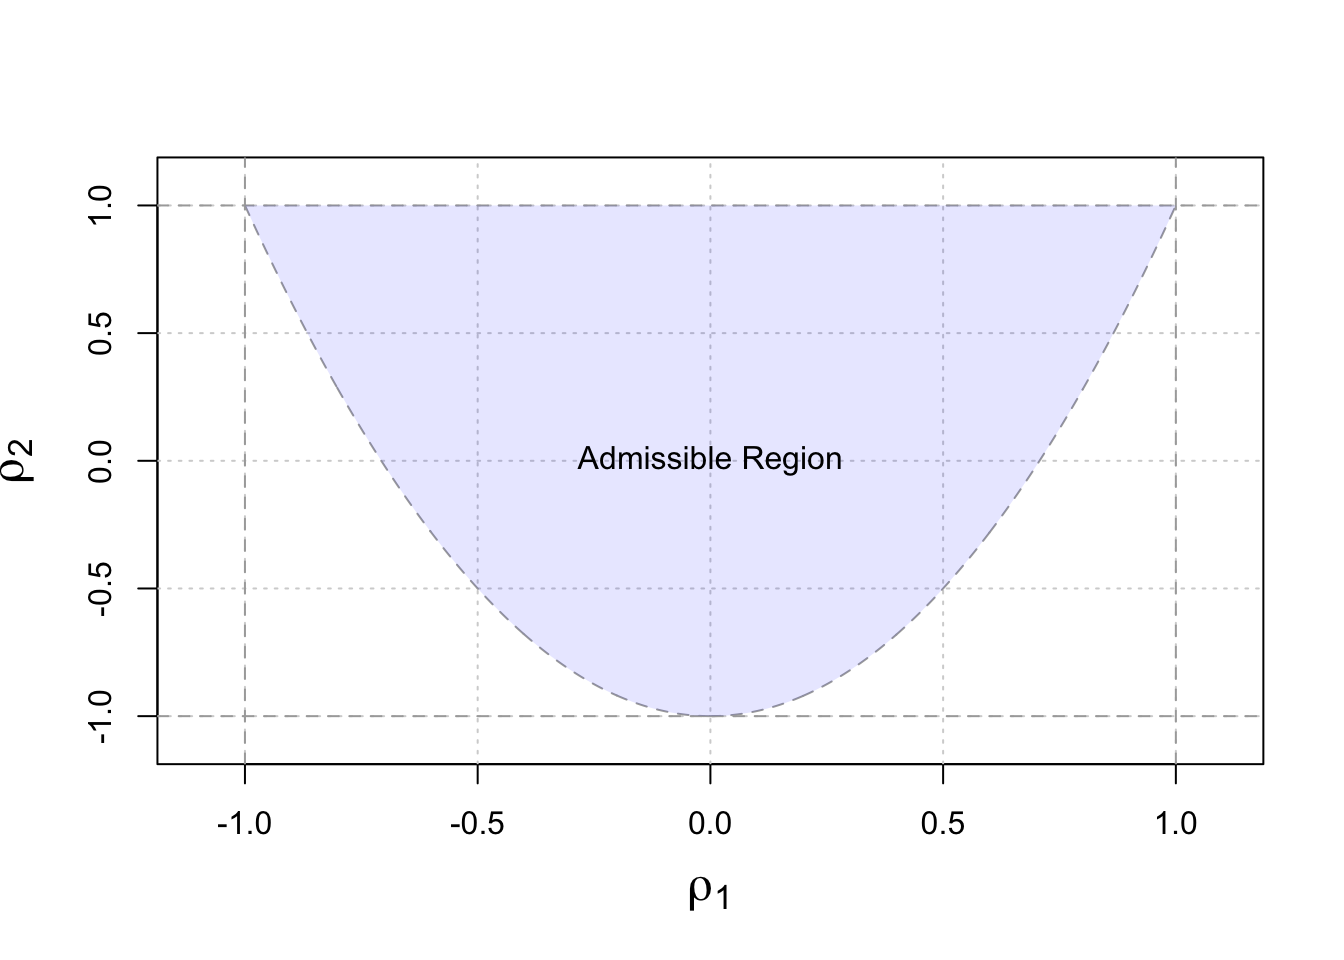
\includegraphics{tts_files/figure-latex/admissibility-1} 

}

\caption{Admissible autocorrelation functions}\label{fig:admissibility}
\end{figure}

From our derivation, it is clear that the restrictions on the
autocorrelation are very complicated, thereby justifying the need for
other forms of fundamental representation which we will explore later in
this text. Before moving on to the estimation of the autocorrelation and
autocovariance functions, we must first discuss the stationarity of
\((X_t)\), which will provide a convenient framework in which
\(\gamma(h)\) and \(\rho(h)\) can be used (rather that \(\gamma(t,t+h)\)
for example) and (easily) estimated.

\hypertarget{stationary}{%
\section{Stationarity}\label{stationary}}

There are two kinds of stationarity that are commonly used. They are
defined as follows:

\BeginKnitrBlock{definition}
\protect\hypertarget{def:strongstationarity}{}{\label{def:strongstationarity}
}A process \((X_t)\) is \emph{strongly stationary} or \emph{strictly
stationary} if the joint probability distribution of
\((X_{t-h}, ..., X_t, ..., X_{t+h})\) is independent of \(t\) for all
\(h\).
\EndKnitrBlock{definition}

\BeginKnitrBlock{definition}
\protect\hypertarget{def:weakstationarity}{}{\label{def:weakstationarity} }A
process \((X_t)\) is \emph{weakly stationary}, \emph{covariance
stationary} or \emph{second order stationary} if \(\mathbb{E}[X_t]\),
\(\mathbb{E}[X_t^2]\) are finite and \(\mathbb{E}[X_t X_{t-h}]\) depends
only on \(h\) and not on \(t\).
\EndKnitrBlock{definition}

These types of stationarity are \emph{not equivalent} and the presence
of one kind of stationarity does not imply the other. That is, a time
series can be strongly stationary but not weakly stationary and vice
versa. In some cases, a time series can be both strongly and weakly
stationary and this is occurs, for example, in the (jointly) Gaussian
case. Stationarity of \((X_t)\) matters because \emph{it provides the
framework in which averaging dependent data makes sense}, thereby
allowing us to easily obtain estimates for certain quantities such as
autocorrelation.

Several remarks and comments can be made on these definitions:

\begin{itemize}
\tightlist
\item
  As mentioned earlier, strong stationarity \emph{does not imply} weak
  stationarity.
\end{itemize}

\BeginKnitrBlock{example}
\protect\hypertarget{exm:strongnotweak}{}{\label{exm:strongnotweak} }an
\(iid\) Cauchy process is strongly but not weakly stationary.
\EndKnitrBlock{example}

\begin{itemize}
\tightlist
\item
  Weak stationarity \emph{does not imply} strong stationarity.
\end{itemize}

\BeginKnitrBlock{example}
\protect\hypertarget{exm:weaksplit}{}{\label{exm:weaksplit} }Consider the
following weak white noise process: \begin{equation*}
X_t = \begin{cases}
U_{t}      & \quad \text{if } t \in \{2k:\, k\in \mathbb{Z} \}, \\
V_{t}      & \quad \text{if } t \in \{2k+1:\, k\in \mathbb{Z} \},\\
\end{cases}
\end{equation*} where
\({U_t} \mathop \sim \limits^{iid} N\left( {1,1} \right)\) and
\({V_t}\mathop \sim \limits^{iid} \mathcal{E}\left( 1 \right)\) is a
weakly stationary process that is \emph{not} strongly stationary.
\EndKnitrBlock{example}

\begin{itemize}
\tightlist
\item
  Strong stationarity combined with bounded values \(\mathbb{E}[X_t]\)
  and \(\mathbb{E}[X_t^2]\) \emph{implies} weak stationarity.
\item
  Weak stationarity combined with normally distributed processes
  \emph{implies} strong stationarity.
\end{itemize}

\hypertarget{assessing-weak-stationarity-of-time-series-models}{%
\subsection{Assessing Weak Stationarity of Time Series
Models}\label{assessing-weak-stationarity-of-time-series-models}}

It is important to understand how to verify if a postulated model is
(weakly) stationary. In order to do so, we must ensure that our model
satisfies the following three properties:

\begin{enumerate}
\def\labelenumi{\arabic{enumi}.}
\tightlist
\item
  \(\mathbb{E}\left[X_t \right] = \mu_t = \mu < \infty\),
\item
  \(\text{var}\left[X_t \right] = \sigma^2_t = \sigma^2 < \infty\),
\item
  \(\text{cov}\left(X_t, X_{t+h} \right) = \gamma \left(h\right)\).
\end{enumerate}

In the following examples, we evaluate the stationarity of the processes
introduced in Section \ref{basicmodels}.

\BeginKnitrBlock{example}[Gaussian White Noise]
\protect\hypertarget{exm:gwn}{}{\label{exm:gwn} \iffalse (Gaussian White
Noise) \fi{} }It is easy to verify that this process is stationary.
Indeed, we have:

\begin{enumerate}
\def\labelenumi{\arabic{enumi}.}
\tightlist
\item
  \(\mathbb{E}\left[ {{X_t}} \right] = 0\),
\item
  \(\gamma(0) = \sigma^2 < \infty\),\\
\item
  \(\gamma(h) = 0\) for \(|h| > 0\).
\end{enumerate}
\EndKnitrBlock{example}

\BeginKnitrBlock{example}[Random Walk]
\protect\hypertarget{exm:srw}{}{\label{exm:srw} \iffalse (Random Walk) \fi{}
}To evaluate the stationarity of this process, we first derive its
properties:

\begin{enumerate}
\def\labelenumi{\arabic{enumi}.}
\tightlist
\item
  We begin by calculating the expectation of the process: \[
    \mathbb{E}\left[ {{X_t}} \right] = \mathbb{E}\left[ {{X_{t - 1}} + {W_t}} \right]
    = \mathbb{E}\left[ {\sum\limits_{i = 1}^t {{W_i}}  + {X_0}} \right] 
    = \mathbb{E}\left[ {\sum\limits_{i = 1}^t {{W_i}} } \right] + {c} 
    = c.  \]
\end{enumerate}

Observe that the mean obtained is constant since it depends only on the
value of the first term in the sequence.

\begin{enumerate}
\def\labelenumi{\arabic{enumi}.}
\setcounter{enumi}{1}
\item
  Next, after finding the mean to be constant, we calculate the variance
  to check stationarity: \[\begin{aligned}
    \text{var}\left( {{X_t}} \right) &= \text{var}\left( {\sum\limits_{i = 1}^t {{W_t}}  + {X_0}} \right) 
    = \text{var}\left( {\sum\limits_{i = 1}^t {{W_i}} } \right) + \underbrace {\text{var}\left( {{X_0}} \right)}_{= 0} \\
    &= \sum\limits_{i = 1}^t {\text{var}\left( {{W_i}} \right)} 
    = t \sigma_w^2,
    \end{aligned}\] where \(\sigma_w^2 = \text{var}(W_t)\). Therefore,
  the variance depends on time \(t\), contradicting our second property.
  Moreover, we have:
  \[\mathop {\lim }\limits_{t \to \infty } \; \text{var}\left(X_t\right) = \infty.\]
  This process is therefore not weakly stationary.
\item
  Regarding the autocovariance of a random walk, we have:
  \[\begin{aligned}
    \gamma \left( h \right) &= \text{cov}\left( {{X_t},{X_{t + h}}} \right) 
    = \text{cov}\left( {\sum\limits_{i = 1}^t {{W_i}} ,\sum\limits_{j = 1}^{t + h} {{W_j}} } \right) 
    = \text{cov}\left( {\sum\limits_{i = 1}^t {{W_i}} ,\sum\limits_{j = 1}^t {{W_j}} } \right)\\ 
    &= \min \left( {t,t + h} \right)\sigma _w^2
    = \left( {t + \min \left( {0,h} \right)} \right)\sigma _w^2,
    \end{aligned} \] which further illustrates the non-stationarity of
  this process.
\end{enumerate}

Moreover, the autocorrelation of this process is given by

\[\rho (h) = \frac{t + \min \left( {0,h} \right)}{\sqrt{t}\sqrt{t+h}},\]

implying (for a fixed \(h\)) that

\[\mathop {\lim }\limits_{t \to \infty } \; \rho(h) = 1.\]
\EndKnitrBlock{example}

In the following simulated example, we illustrate the non-stationary
feature of such a process:

\begin{Shaded}
\begin{Highlighting}[]
\CommentTok{# Number of simulated processes}
\NormalTok{B =}\StringTok{ }\DecValTok{200}

\CommentTok{# Length of random walks}
\NormalTok{n =}\StringTok{ }\DecValTok{1000}

\CommentTok{# Output matrix}
\NormalTok{out =}\StringTok{ }\KeywordTok{matrix}\NormalTok{(}\OtherTok{NA}\NormalTok{,B,n)}

\CommentTok{# Set seed for reproducibility}
\KeywordTok{set.seed}\NormalTok{(}\DecValTok{6182}\NormalTok{)}

\CommentTok{# Simulate Data}
\ControlFlowTok{for}\NormalTok{ (i }\ControlFlowTok{in} \KeywordTok{seq_len}\NormalTok{(B))\{}
  \CommentTok{# Simulate random walk}
\NormalTok{  Xt =}\StringTok{ }\KeywordTok{gen_gts}\NormalTok{(n, }\KeywordTok{RW}\NormalTok{(}\DataTypeTok{gamma =} \DecValTok{1}\NormalTok{))}
  
  \CommentTok{# Store process}
\NormalTok{  out[i,] =}\StringTok{ }\NormalTok{Xt}
\NormalTok{\}}

\CommentTok{# Plot random walks}
\KeywordTok{plot}\NormalTok{(}\OtherTok{NA}\NormalTok{, }\DataTypeTok{xlim =} \KeywordTok{c}\NormalTok{(}\DecValTok{1}\NormalTok{,n), }\DataTypeTok{ylim =} \KeywordTok{range}\NormalTok{(out), }\DataTypeTok{xlab =} \StringTok{"Time"}\NormalTok{, }\DataTypeTok{ylab =} \StringTok{" "}\NormalTok{)}
\KeywordTok{grid}\NormalTok{()}
\NormalTok{color =}\StringTok{ }\KeywordTok{sample}\NormalTok{(}\KeywordTok{topo.colors}\NormalTok{(B, }\DataTypeTok{alpha =} \FloatTok{0.5}\NormalTok{))}
\KeywordTok{grid}\NormalTok{()}
\ControlFlowTok{for}\NormalTok{ (i }\ControlFlowTok{in} \KeywordTok{seq_len}\NormalTok{(B))\{}
  \KeywordTok{lines}\NormalTok{(out[i,], }\DataTypeTok{col =}\NormalTok{ color[i])}
\NormalTok{\}}

\CommentTok{# Add 95% confidence region}
\KeywordTok{lines}\NormalTok{(}\DecValTok{1}\OperatorTok{:}\NormalTok{n, }\FloatTok{1.96}\OperatorTok{*}\KeywordTok{sqrt}\NormalTok{(}\DecValTok{1}\OperatorTok{:}\NormalTok{n), }\DataTypeTok{col =} \DecValTok{2}\NormalTok{, }\DataTypeTok{lwd =} \DecValTok{2}\NormalTok{, }\DataTypeTok{lty =} \DecValTok{2}\NormalTok{)}
\KeywordTok{lines}\NormalTok{(}\DecValTok{1}\OperatorTok{:}\NormalTok{n, }\FloatTok{-1.96}\OperatorTok{*}\KeywordTok{sqrt}\NormalTok{(}\DecValTok{1}\OperatorTok{:}\NormalTok{n), }\DataTypeTok{col =} \DecValTok{2}\NormalTok{, }\DataTypeTok{lwd =} \DecValTok{2}\NormalTok{, }\DataTypeTok{lty =} \DecValTok{2}\NormalTok{)}
\end{Highlighting}
\end{Shaded}

\begin{figure}

{\centering 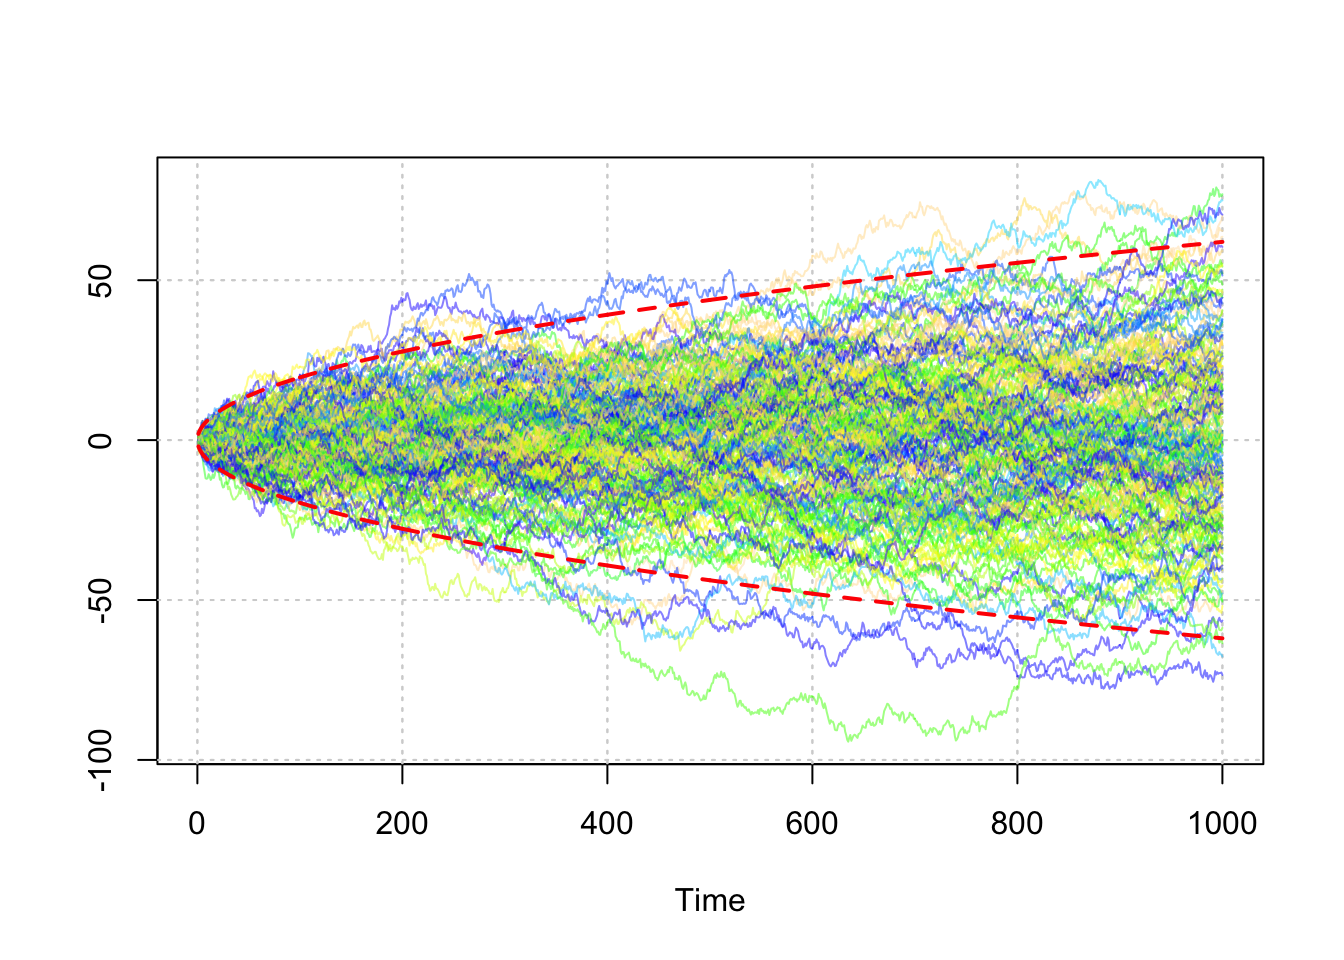
\includegraphics{tts_files/figure-latex/RWsim-1} 

}

\caption{Two hundred simulated random walks.}\label{fig:RWsim}
\end{figure}

In the plot above, two hundred simulated random walks are plotted along
with theoretical 95\% confidence intervals (red-dashed lines). The
relationship between time and variance can clearly be observed (i.e.~the
variance of the process increases with the time).

\BeginKnitrBlock{example}[Moving Average of Order 1]
\protect\hypertarget{exm:exma1}{}{\label{exm:exma1} \iffalse (Moving Average
of Order 1) \fi{} } Similarly to our previous examples, we attempt to
verify the stationary properties for the MA(1) model defined in Section
\ref{ma1}:

\begin{enumerate}
\def\labelenumi{\arabic{enumi}.}
\tightlist
\item
  \[ 
   \mathbb{E}\left[ {{X_t}} \right] = \mathbb{E}\left[ {{\theta_1}{W_{t - 1}} + {W_t}} \right] 
   = {\theta_1} \mathbb{E} \left[ {{W_{t - 1}}} \right] + \mathbb{E}\left[ {{W_t}} \right] 
   = 0. \]
\item
  \[\text{var} \left( {{X_t}} \right) = \theta_1^2 \text{var} \left( W_{t - 1}\right) + \text{var} \left( W_{t}\right) = \left(1 + \theta^2 \right) \sigma^2_w.\]\\
\item
  Regarding the autocovariance, we have \[\begin{aligned}
  \text{cov}\left( {{X_t},{X_{t + h}}} \right) &= \mathbb{E}\left[ {\left( {{X_t} - \mathbb{E}\left[ {{X_t}} \right]} \right)\left( {{X_{t + h}} - \mathbb{E}\left[ {{X_{t + h}}} \right]} \right)} \right] = \mathbb{E}\left[ {{X_t}{X_{t + h}}} \right] \\
  &= \mathbb{E}\left[ {\left( {{\theta}{W_{t - 1}} + {W_t}} \right)\left( {{\theta }{W_{t + h - 1}} + {W_{t + h}}} \right)} \right] \\
  &= \mathbb{E}\left[ {\theta^2{W_{t - 1}}{W_{t + h - 1}} + \theta {W_t}{W_{t + h}} + {\theta}{W_{t - 1}}{W_{t + h}} + {W_t}{W_{t + h}}} \right]. \\
  \end{aligned} \] It is easy to see that
  \(\mathbb{E}\left[ {{W_t}{W_{t + h}}} \right] = {\boldsymbol{1}_{\left\{ {h = 0} \right\}}}\sigma _w^2\)
  and therefore, we obtain
  \[\text{cov} \left( {{X_t},{X_{t + h}}} \right) = \left( {\theta^2{ \boldsymbol{1}_{\left\{ {h = 0} \right\}}} + {\theta}{\boldsymbol{1}_{\left\{ {h = 1} \right\}}} + {\theta}{\boldsymbol{1}_{\left\{ {h =  - 1} \right\}}} + {\boldsymbol{1}_{\left\{ {h = 0} \right\}}}} \right)\sigma _w^2\]
  implying the following autocovariance function:
  \[\gamma \left( h \right) = \left\{ {\begin{array}{*{20}{c}}
   {\left( {\theta^2 + 1} \right)\sigma _w^2}&{h = 0} \\ 
   {{\theta}\sigma _w^2}&{\left| h \right| = 1} \\ 
   0&{\left| h \right| > 1} 
   \end{array}} \right. .\] Therefore, an MA(1) process is weakly
  stationary since both the mean and variance are constant over time and
  its covariance function is only a function of the lag \((h)\).
  Finally, we can easily obtain the autocorrelation for this process,
  which is given by
  \[\rho \left( h \right) = \left\{ {\begin{array}{*{20}{c}}
    1&{h = 0} \\ 
    {\frac{{{\theta}\sigma _w^2}}{{\left( {\theta^2 + 1} \right)\sigma _w^2}} = \frac{{{\theta}}}{{\theta^2 + 1}}}&{\left| h \right| = 1} \\ 
    0&{\left| h \right| > 1} 
    \end{array}} \right. .\] Interestingly, we can note that
  \(|\rho(1)| \leq 0.5\).

  \EndKnitrBlock{example}
\end{enumerate}

\BeginKnitrBlock{example}[Autoregressive of Order 1]
\protect\hypertarget{exm:exar1}{}{\label{exm:exar1} \iffalse (Autoregressive
of Order 1) \fi{} } As another example, we shall verify the stationary
properties for the AR(1) model defined in Section \ref{ar1}.

Using the \emph{backsubstitution} technique, we can rearrange an AR(1)
process so that it is written in a more compact form, i.e.

\[\begin{aligned}
     {X_t} & =  {\phi }{X_{t - 1}} + {W_t} = \phi \left[ {\phi {X_{t - 2}} + {W_{t - 1}}} \right] + {W_t} 
     =  {\phi ^2}{X_{t - 2}} + \phi {W_{t - 1}} + {W_t}  \\
     &  \vdots  \\
     & =  {\phi ^k}{X_{t-k}} + \sum\limits_{j = 0}^{k - 1} {{\phi ^j}{W_{t - j}}} .
     \end{aligned} \]

By taking the limit in \(k\) (which is perfectly valid as we assume
\(t \in \mathbb{Z}\)) and assuming \(|\phi|<1\), we obtain

\[\begin{aligned}
     X_t = \mathop {\lim }\limits_{k \to \infty} \; {X_t}  =  \sum\limits_{j = 0}^{\infty} {{\phi ^j}{W_{t - j}}} 
     \end{aligned} \]

and therefore such process can be interpreted as a linear combination of
the white noise \((W_t)\) and corresponds (as we will observe later on)
to an MA(\(\infty\)). In addition, the requirement
\(\left| \phi \right| < 1\) turns out to be extremely useful as the
above formula is related to a \textbf{geometric series}, which would
diverge if \(\phi \geq 1\). Indeed, remember that an infinite
(converging) geometric series is given by

\[\sum\limits_{k = 0}^\infty  \, a{{r^k}}  = \frac{a}{{1 - r}}, \; {\text{ if }}\left| r \right| < 1.\]

With this setup, we demonstrate how crucial this property is by
calculating each of the requirements of a stationary process.

\begin{enumerate}
\def\labelenumi{\arabic{enumi}.}
\tightlist
\item
  First, we will check if the mean is stationary. In this case, we opt
  to use limits to derive the expectation \[\begin{aligned}
  \mathbb{E}\left[ {{X_t}} \right] &= \mathop {\lim }\limits_{k \to \infty } \mathbb{E}\left[ {{\phi^k}{X_{t-k}} + \sum\limits_{j = 0}^{k - 1} {\phi^j{W_{t - j}}} } \right] \\
  &= \mathop {\lim }\limits_{k \to \infty } \, \underbrace {{\phi ^k}{\mathbb{E}[X_{t-k}]}}_{= 0} + \mathop {\lim }\limits_{k \to \infty } \, \sum\limits_{j = 0}^{k - 1} {\phi^j\underbrace {\mathbb{E}\left[ {{W_{t - j}}} \right]}_{ = 0}}
  = 0.
  \end{aligned} \] As expected, the mean is zero and, hence, the first
  criteria for weak stationarity is satisfied.
\item
  Next, we opt to determine the variance of the process
  \[\begin{aligned}
  \text{var}\left( {{X_t}} \right) &= \mathop {\lim }\limits_{k \to \infty } \text{var}\left( {{\phi^k}{X_{t-k}} + \sum\limits_{j = 0}^{k - 1} {\phi^j{W_{t - j}}} } \right)
  = \mathop {\lim }\limits_{k \to \infty } \sum\limits_{j = 0}^{k - 1} {\phi ^{2j} \text{var}\left( {{W_{t - j}}} \right)}  \\
  &= \mathop {\lim }\limits_{k \to \infty } \sum\limits_{j = 0}^{k - 1} \sigma _W^2 \, {\phi ^{2j}}  =  
    \underbrace {\frac{\sigma _W^2}{{1 - {\phi ^2}}}.}_{\begin{subarray}{l} 
      {\text{Geom. Serie}} 
      \end{subarray}}
  \end{aligned} \] Once again, the above result only holds because we
  are able to use the geometric series convergence as a result of
  \(\left| \phi \right| < 1\).
\item
  Finally, we consider the autocovariance of an AR(1). For \(h > 0\), we
  have
  \[\gamma \left( h \right) =  \text{cov}\left( {{X_t},{X_{t + h}}} \right) = \phi \text{cov}\left( {{X_t},{X_{t + h - 1}}} \right) = \phi \, \gamma \left( h-1 \right).\]
  Therefore, using the symmetry of autocovariance, we find that
  \[\gamma \left( h \right) = \phi^{|h|} \, \gamma(0).\]
\end{enumerate}

Both the mean and variance do not depend on time. In addition, the
autocovariance function can be viewed as a function dependent entirely
on lags and, thus, the AR(1) process is weakly stationary if
\(\left| \phi \right| < 1\). Lastly, we can obtain the autocorrelation
for this process. Indeed, for \(h > 0\), we have

\[\rho \left( h \right) = \frac{{\gamma \left( h \right)}}{{\gamma \left( 0 \right)}} = \frac{{\phi \gamma \left( {h - 1} \right)}}{{\gamma \left( 0 \right)}} = \phi \rho \left( {h - 1} \right).\]

After fully simplifying, we obtain

\[\rho \left( h \right) = {\phi^{|h|}}.\]

Thus, the autocorrelation function for an AR(1) exhibits a
\emph{geometric decay}, meaning, the smaller the \(|\phi|\), the faster
the autocorrelation reaches zero. If \(|\phi|\) is close to 1, then the
decay rate is slower.
\EndKnitrBlock{example}

\hypertarget{estimation-of-moments-of-stationary-processes}{%
\section{Estimation of Moments of Stationary
Processes}\label{estimation-of-moments-of-stationary-processes}}

In this section, we discuss how moments and related quantities of
stationary process can be estimated. Informally speaking, the use of
``averages'' is meaningful for such processes suggesting that classical
moments estimators can be employed. Indeed, suppose that one is
interested in estimating \(\alpha \equiv \mathbb{E}[m (X_t)]\), where
\(m(\cdot)\) is a known function of \(X_t\). If \(X_t\) is a strongly
stationary process, we have

\[\alpha = \int m(x) \, f(x) dx\]

where \(f(x)\) denotes the density of \(X_t, \; \forall t\). Replacing
\(f(x)\) by \(f_n(x)\), the empirical density, we obtain the following
estimator

\[\hat{\alpha} = \frac{1}{n} \sum_{i = 1}^n m\left(x_i\right).\]

In the next subsection, we examine how this simple idea can be used to
estimate the mean, autocovariance and autocorrelation functions.
Moreover, we discuss some of the properties of these estimators.

\hypertarget{estimation-of-the-mean-function}{%
\subsection{Estimation of the Mean
Function}\label{estimation-of-the-mean-function}}

If a time series is stationary, the mean function is constant and a
possible estimator of this quantity is, as discussed above, given by

\[\bar{X} = {\frac{1}{n}\sum\limits_{t = 1}^n {{X_t}} }.\]

Naturally, the \(k\)-th moment, say \(\beta_k \equiv \mathbb{E}[X_t^k]\)
can be estimated by

\[\hat{\beta}_k = {\frac{1}{n}\sum\limits_{t = 1}^n {{X_t^k}} }, \;\; k \in \left\{x \in \mathbb{N} : \, 0 < x < \infty  \right\}.\]

The variance of such an estimator can be derived as follows:

\begin{equation}
  \begin{aligned}
  \text{var} \left( \hat{\beta}_k \right) &= \text{var} \left( {\frac{1}{n}\sum\limits_{t = 1}^n {{X_t^k}} } \right)  \\
  &= \frac{1}{{{n^2}}}\text{var} \left( {{{\left[ {\begin{array}{*{20}{c}}
    1& \cdots &1
    \end{array}} \right]}_{1 \times n}}{{\left[ {\begin{array}{*{20}{c}}
      {{X_1^k}} \\
      \vdots  \\
      {{X_n^k}}
      \end{array}} \right]}_{n \times 1}}} \right)  \\
  &= \frac{1}{{{n^2}}}{\left[ {\begin{array}{*{20}{c}}
    1& \cdots &1
    \end{array}} \right]_{1 \times n}} \, \boldsymbol{\Sigma}(k) \, {\left[ {\begin{array}{*{20}{c}}
      1 \\
      \vdots  \\
      1
      \end{array}} \right]_{n \times 1}}, 
  \end{aligned}
  \label{eq:chap2VarMoment}
\end{equation}

where \(\boldsymbol{\Sigma}(k) \in \mathbb{R}^{n \times n}\) and its
\(i\)-th, \(j\)-th element is given by

\[ \left(\boldsymbol{\Sigma}(k)\right)_{i,j} = \text{cov} \left(X_i^k, X_j^k\right).\]

In the case \(k = 1\), \eqref{eq:chap2VarMoment} can easily be further
simplified. Indeed, we have

\[\begin{aligned}
       \text{var} \left( {\bar X} \right) &= \text{var} \left( {\frac{1}{n}\sum\limits_{t = 1}^n {{X_t}} } \right)  \\
       &= \frac{1}{{{n^2}}}{\left[ {\begin{array}{*{20}{c}}
         1& \cdots &1
         \end{array}} \right]_{1 \times n}}\left[ {\begin{array}{*{20}{c}}
           {\gamma \left( 0 \right)}&{\gamma \left( 1 \right)}& \cdots &{\gamma \left( {n - 1} \right)} \\
           {\gamma \left( 1 \right)}&{\gamma \left( 0 \right)}&{}& \vdots  \\
           \vdots &{}& \ddots & \vdots  \\
           {\gamma \left( {n - 1} \right)}& \cdots & \cdots &{\gamma \left( 0 \right)}
           \end{array}} \right]_{n \times n}{\left[ {\begin{array}{*{20}{c}}
             1 \\
             \vdots  \\
             1
             \end{array}} \right]_{n \times 1}}  \\
       &= \frac{1}{{{n^2}}}\left( {n\gamma \left( 0 \right) + 2\left( {n - 1} \right)\gamma \left( 1 \right) + 2\left( {n - 2} \right)\gamma \left( 2 \right) +  \cdots  + 2\gamma \left( {n - 1} \right)} \right)  \\
       &= \frac{1}{n}\sum\limits_{h =  - n}^n {\left( {1 - \frac{{\left| h \right|}}{n}} \right)\gamma \left( h \right)} .  \\
\end{aligned} \]

Obviously, when \(X_t\) is a white noise process, the above formula
reduces to the usual
\(\text{var} \left( {\bar X} \right) = \sigma^2_w/n\). In the following
example, we consider the case of an AR(1) process and discuss how
\(\text{var} \left( {\bar X} \right)\) can be obtained or estimated.

\BeginKnitrBlock{example}
\protect\hypertarget{exm:exactvbootstrap}{}{\label{exm:exactvbootstrap} }For
an AR(1), we have
\(\gamma(h) = \phi^h \sigma_w^2 \left(1 - \phi^2\right)^{-1}\).
Therefore, we obtain (after some computations):

\begin{equation}
    \text{var} \left( {\bar X} \right) = \frac{\sigma_w^2 \left( n - 2\phi - n \phi^2 + 2 \phi^{n + 1}\right)}{n^2\left(1-\phi^2\right)\left(1-\phi\right)^2}.
\end{equation}

Unfortunately, deriving such an exact formula is often difficult when
considering more complex models. However, asymptotic approximations are
often employed to simplify the calculation. For example, in our case we
have

\[\mathop {\lim }\limits_{n \to \infty } \; n \text{var} \left( {\bar X} \right) = \frac{\sigma_w^2}{\left(1-\phi\right)^2},\]

providing the following approximate formula:

\[\text{var} \left( {\bar X} \right) \approx \frac{\sigma_w^2}{n \left(1-\phi\right)^2}.\]

Alternatively, simulation methods can also be employed. For example, a
possible strategy would be parametric bootstrap.
\EndKnitrBlock{example}

\BeginKnitrBlock{theorem}
\protect\hypertarget{thm:parabootstrap}{}{\label{thm:parabootstrap} }1.
Simulate a new sample under the postulated model, i.e.
\(X_t^* \sim F_{\boldsymbol{theta}}{\) (\emph{note:} if
\(\boldsymbol{theta}\) is unknown it can be replace by
\(\hat{\boldsymbol{theta}}\), a suitable estimator). 2. Compute the
statistics of interest on the simulated sample \((X_t^*)\). 3. Repeat
Steps 1 and 2 \(B\) times where \(B\) is sufficiently ``large''
(typically \(100 \leq B \leq 10000\)). 4. Compute the empirical variance
of the statistics of interest based on the \(B\) independent
replications.
\EndKnitrBlock{theorem}

In our example, we would consider \((X_t^*)\) to be \({\bar{X}^*}\) and
seek to obtain:

\[\hat{\sigma}^2_B = \frac{1}{B-1} \sum_{i = 1}^B \left(\bar{X}^*_i - \bar{X}^* \right)^2, \;\;\; \text{where} \;\;\; \bar{X}^* = \frac{1}{B} \sum_{i=1}^B \bar{X}^*_i,\]

where \(\bar{X}^*_i\) denotes the value of the mean estimated on the
\(i\)-th simulated sample.

The figure below generated by the following code compares these three
methods for \(n = 10\), \(B = 1000\), \(\sigma^2 = 1\) and a grid of
values for \(\phi\) going from \(-0.95\) to \(0.95\):

\begin{Shaded}
\begin{Highlighting}[]
\CommentTok{# Define sample size}
\NormalTok{n =}\StringTok{ }\DecValTok{10}

\CommentTok{# Number of Monte-Carlo replications}
\NormalTok{B =}\StringTok{ }\DecValTok{5000}

\CommentTok{# Define grid of values for phi}
\NormalTok{phi =}\StringTok{ }\KeywordTok{seq}\NormalTok{(}\DataTypeTok{from =} \FloatTok{0.95}\NormalTok{, }\DataTypeTok{to =} \FloatTok{-0.95}\NormalTok{, }\DataTypeTok{length.out =} \DecValTok{30}\NormalTok{)}

\CommentTok{# Define result matrix}
\NormalTok{result =}\StringTok{ }\KeywordTok{matrix}\NormalTok{(}\OtherTok{NA}\NormalTok{,B,}\KeywordTok{length}\NormalTok{(phi))}

\CommentTok{# Start simulation}
\ControlFlowTok{for}\NormalTok{ (i }\ControlFlowTok{in} \KeywordTok{seq_along}\NormalTok{(phi))\{}
  \CommentTok{# Define model}
\NormalTok{  model =}\StringTok{ }\KeywordTok{AR1}\NormalTok{(}\DataTypeTok{phi =}\NormalTok{ phi[i], }\DataTypeTok{sigma2 =} \DecValTok{1}\NormalTok{)}
  
  \CommentTok{# Monte-Carlo}
  \ControlFlowTok{for}\NormalTok{ (j }\ControlFlowTok{in} \KeywordTok{seq_len}\NormalTok{(B))\{}
    \CommentTok{# Simulate AR(1)}
\NormalTok{    Xt =}\StringTok{ }\KeywordTok{gen_gts}\NormalTok{(n, model)}
    
    \CommentTok{# Estimate Xbar}
\NormalTok{    result[j,i] =}\StringTok{ }\KeywordTok{mean}\NormalTok{(Xt)}
\NormalTok{  \}}
\NormalTok{\}}

\CommentTok{# Estimate variance of Xbar}
\NormalTok{var.Xbar =}\StringTok{ }\KeywordTok{apply}\NormalTok{(result,}\DecValTok{2}\NormalTok{,var)}

\CommentTok{# Compute theoretical variance}
\NormalTok{var.theo =}\StringTok{ }\NormalTok{(n }\OperatorTok{-}\StringTok{ }\DecValTok{2}\OperatorTok{*}\NormalTok{phi }\OperatorTok{-}\StringTok{ }\NormalTok{n}\OperatorTok{*}\NormalTok{phi}\OperatorTok{^}\DecValTok{2} \OperatorTok{+}\StringTok{ }\DecValTok{2}\OperatorTok{*}\NormalTok{phi}\OperatorTok{^}\NormalTok{(n}\OperatorTok{+}\DecValTok{1}\NormalTok{))}\OperatorTok{/}\NormalTok{(n}\OperatorTok{^}\DecValTok{2}\OperatorTok{*}\NormalTok{(}\DecValTok{1}\OperatorTok{-}\NormalTok{phi}\OperatorTok{^}\DecValTok{2}\NormalTok{)}\OperatorTok{*}\NormalTok{(}\DecValTok{1}\OperatorTok{-}\NormalTok{phi)}\OperatorTok{^}\DecValTok{2}\NormalTok{)}

\CommentTok{# Compute (approximate) variance}
\NormalTok{var.approx =}\StringTok{ }\DecValTok{1}\OperatorTok{/}\NormalTok{(n}\OperatorTok{*}\NormalTok{(}\DecValTok{1}\OperatorTok{-}\NormalTok{phi)}\OperatorTok{^}\DecValTok{2}\NormalTok{)}

\CommentTok{# Compare variance estimations}
\KeywordTok{plot}\NormalTok{(}\OtherTok{NA}\NormalTok{, }\DataTypeTok{xlim =} \KeywordTok{c}\NormalTok{(}\OperatorTok{-}\DecValTok{1}\NormalTok{,}\DecValTok{1}\NormalTok{), }\DataTypeTok{ylim =} \KeywordTok{range}\NormalTok{(var.approx), }\DataTypeTok{log =} \StringTok{"y"}\NormalTok{, }
     \DataTypeTok{ylab =} \KeywordTok{expression}\NormalTok{(}\KeywordTok{paste}\NormalTok{(}\StringTok{"var("}\NormalTok{, }\KeywordTok{bar}\NormalTok{(X), }\StringTok{")"}\NormalTok{)),}
     \DataTypeTok{xlab=} \KeywordTok{expression}\NormalTok{(phi), }\DataTypeTok{cex.lab =} \DecValTok{1}\NormalTok{)}
\KeywordTok{grid}\NormalTok{()}
\KeywordTok{lines}\NormalTok{(phi,var.theo, }\DataTypeTok{col =} \StringTok{"deepskyblue4"}\NormalTok{)}
\KeywordTok{lines}\NormalTok{(phi, var.Xbar, }\DataTypeTok{col =} \StringTok{"firebrick3"}\NormalTok{)}
\KeywordTok{lines}\NormalTok{(phi,var.approx, }\DataTypeTok{col =} \StringTok{"springgreen4"}\NormalTok{)}
\KeywordTok{legend}\NormalTok{(}\StringTok{"topleft"}\NormalTok{,}\KeywordTok{c}\NormalTok{(}\StringTok{"Theoretical variance"}\NormalTok{,}\StringTok{"Bootstrap variance"}\NormalTok{,}\StringTok{"Approximate variance"}\NormalTok{), }
       \DataTypeTok{col =} \KeywordTok{c}\NormalTok{(}\StringTok{"deepskyblue4"}\NormalTok{,}\StringTok{"firebrick3"}\NormalTok{,}\StringTok{"springgreen4"}\NormalTok{), }\DataTypeTok{lty =} \DecValTok{1}\NormalTok{,}
       \DataTypeTok{bty =} \StringTok{"n"}\NormalTok{,}\DataTypeTok{bg =} \StringTok{"white"}\NormalTok{, }\DataTypeTok{box.col =} \StringTok{"white"}\NormalTok{, }\DataTypeTok{cex =} \FloatTok{1.2}\NormalTok{)}
\end{Highlighting}
\end{Shaded}

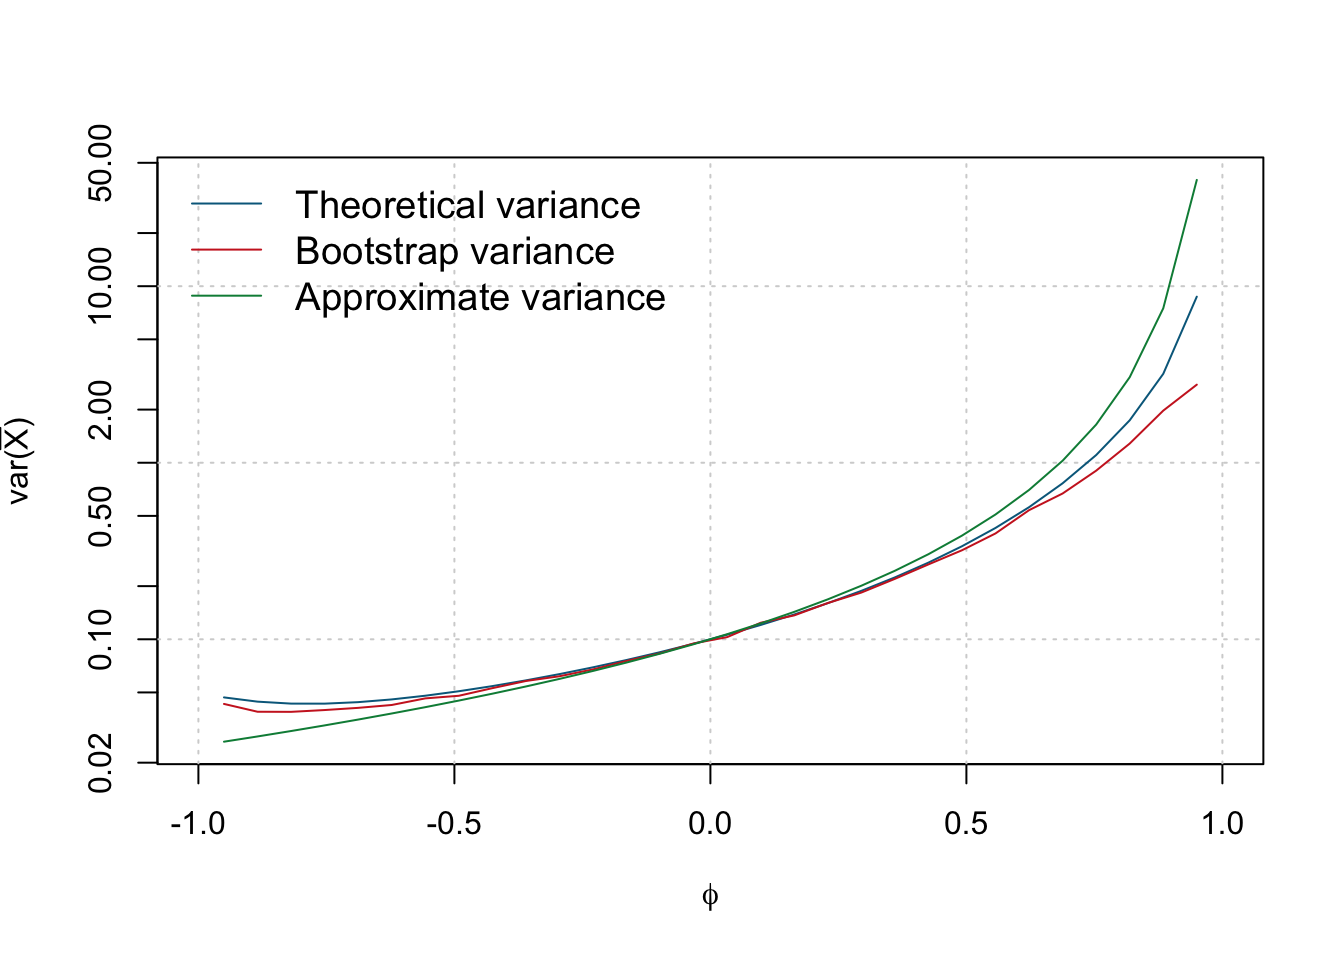
\includegraphics{tts_files/figure-latex/estimXbar-1.pdf}

It can be observed that the variance of \(\bar{X}\) typically increases
with \(\phi\). As expected when \(\phi = 0\), we have
\(\text{var}(\bar{X}) = 1/n\) --- in this case the process is a white
noise. Moreover, the bootstrap approach appears to approximate well the
curve of (@ref(eq:chap2\_exAR1)), while the asymptotic formula provides
a reasonable approximation for \(\phi\) being between -0.5 and 0.5.
Naturally, the quality of this approximation would be far better for a
larger sample size (here we consider \(n = 10\), which is a little
``extreme'').

\hypertarget{sample-autocovariance-and-autocorrelation-functions}{%
\subsection{Sample Autocovariance and Autocorrelation
Functions}\label{sample-autocovariance-and-autocorrelation-functions}}

A natural estimator of the \emph{autocovariance function} is given by:

\[\hat \gamma \left( h \right) = \frac{1}{T}\sum\limits_{t = 1}^{T - h} {\left( {{X_t} - \bar X} \right)\left( {{X_{t + h}} - \bar X} \right)} \]

leading to the following ``plug-in'' estimator of the
\emph{autocorrelation function}:

\[\hat \rho \left( h \right) = \frac{{\hat \gamma \left( h \right)}}{{\hat \gamma \left( 0 \right)}}.\]

A graphical representation of the autocorrelation function is often the
first step for any time series analysis (again assuming the process to
be stationary). Consider the following simulated example:

\begin{Shaded}
\begin{Highlighting}[]
\CommentTok{# Set seed for reproducibility}
\KeywordTok{set.seed}\NormalTok{(}\DecValTok{2241}\NormalTok{)}

\CommentTok{# Simulate 100 observation from a Gaussian white noise}
\NormalTok{Xt =}\StringTok{ }\KeywordTok{gen_gts}\NormalTok{(}\DecValTok{100}\NormalTok{, }\KeywordTok{WN}\NormalTok{(}\DataTypeTok{sigma2 =} \DecValTok{1}\NormalTok{))}

\CommentTok{# Compute autocorrelation}
\NormalTok{acf_Xt =}\StringTok{ }\KeywordTok{ACF}\NormalTok{(Xt)}

\CommentTok{# Plot autocorrelation}
\KeywordTok{plot}\NormalTok{(acf_Xt, }\DataTypeTok{show.ci =} \OtherTok{FALSE}\NormalTok{)}
\end{Highlighting}
\end{Shaded}

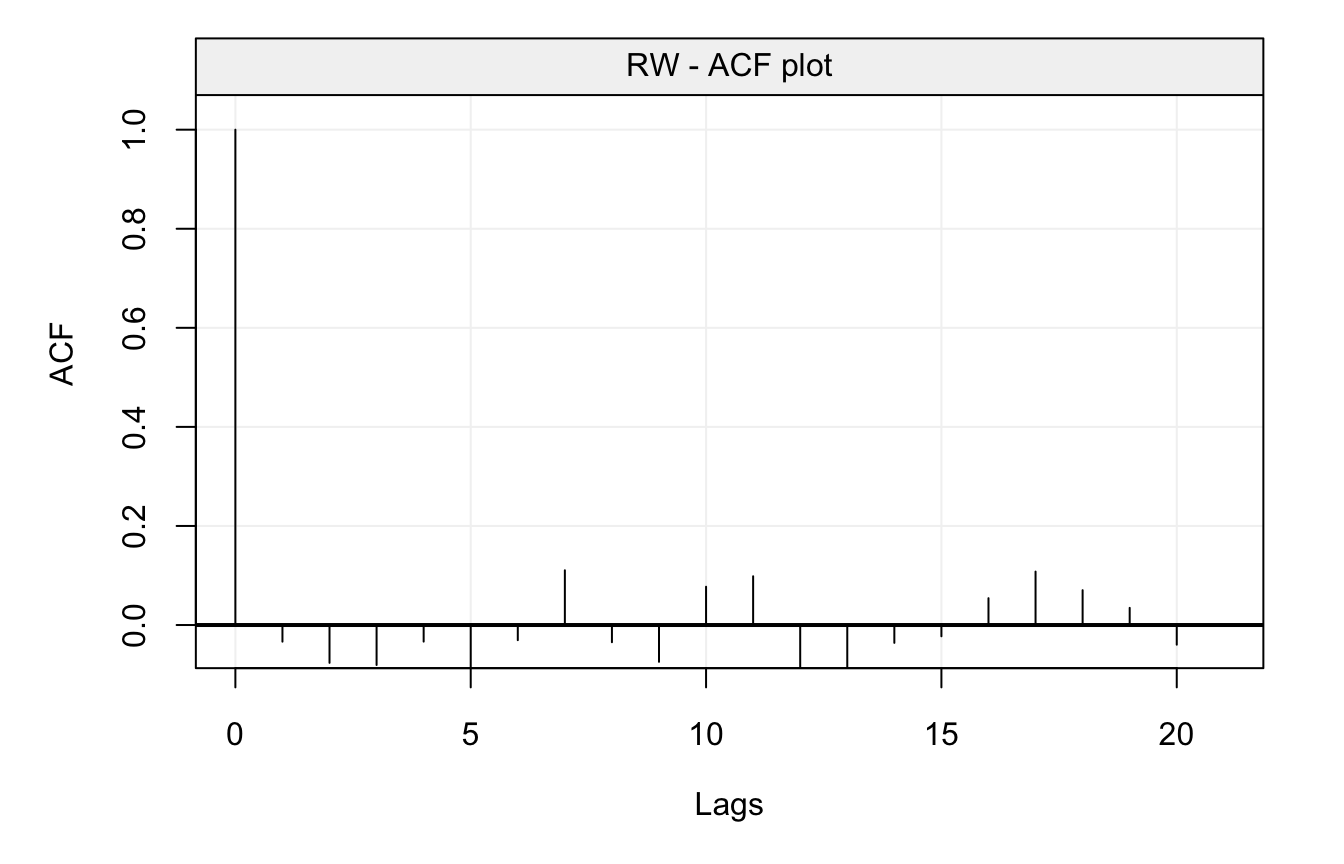
\includegraphics{tts_files/figure-latex/basicACF-1.pdf}

In this example, the true autocorrelation is equal to zero at any lag
\(h \neq 0\), but obviously the estimated autocorrelations are random
variables and are not equal to their true values. It would therefore be
useful to have some knowledge about the variability of the sample
autocorrelations (under some conditions) to assess whether the data
comes from a completely random series or presents some significant
correlation at certain lags. The following result provides an asymptotic
solution to this problem:

\BeginKnitrBlock{theorem}
\protect\hypertarget{thm:approxnormal}{}{\label{thm:approxnormal} }If
\(X_t\) is a strong white noise with finite fourth moment, then
\(\hat{\rho}(h)\) is approximately normally distributed with mean \(0\)
and variance \(n^{-1}\) for all fixed \(h\).
\EndKnitrBlock{theorem}

The proof of this Theorem is given in Appendix \ref{appendixa}.

Using this result, we now have an approximate method to assess whether
peaks in the sample autocorrelation are significant by determining
whether the observed peak lies outside the interval \(\pm 2/\sqrt{T}\)
(i.e.~an approximate 95\% confidence interval). Returning to our
previous example and adding confidence bands to the previous graph, we
obtain:

\begin{Shaded}
\begin{Highlighting}[]
\CommentTok{# Plot autocorrelation with confidence bands }
\KeywordTok{plot}\NormalTok{(acf_Xt)}
\end{Highlighting}
\end{Shaded}

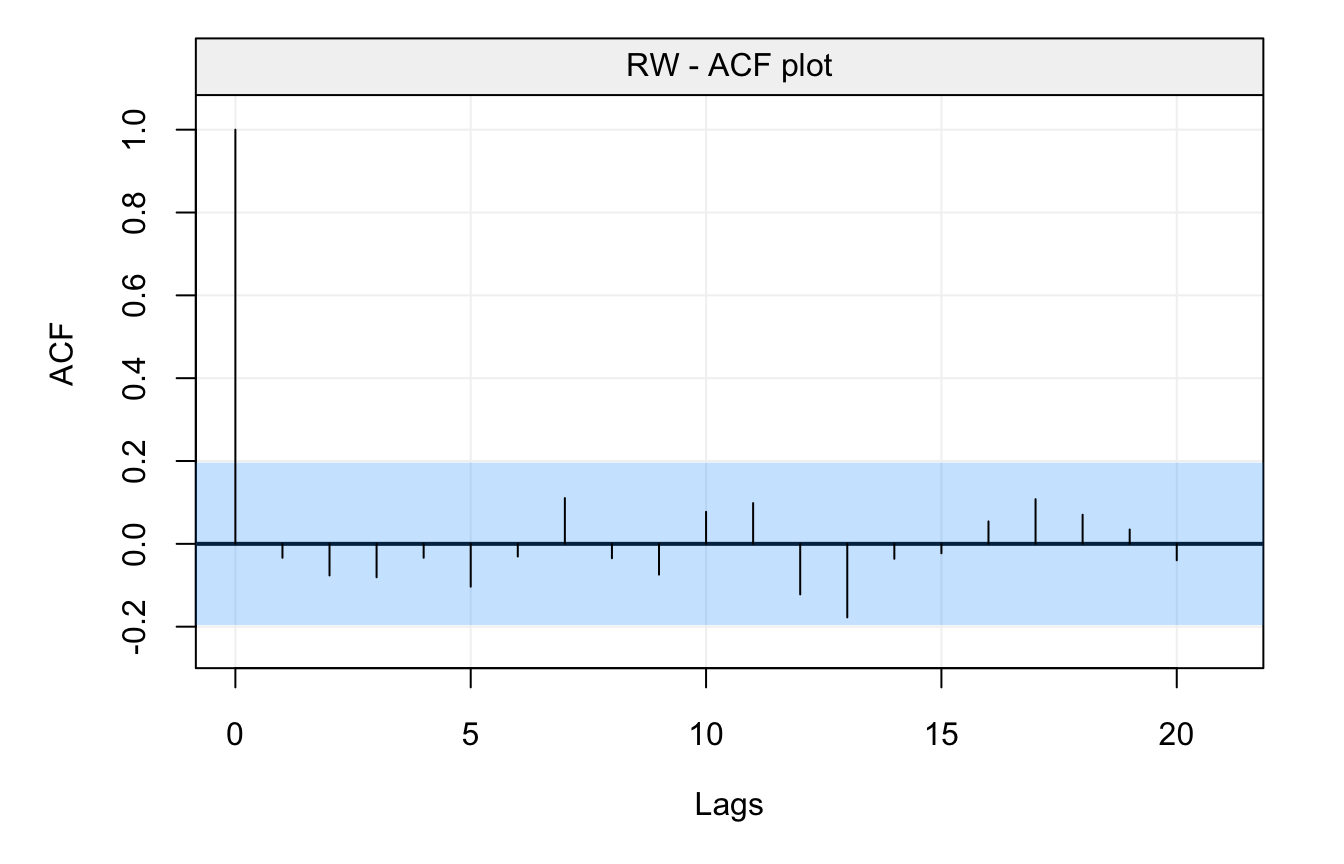
\includegraphics{tts_files/figure-latex/basicACF2-1.pdf}

It can now be observed that most peaks lie within the interval
\(\pm 2/\sqrt{T}\) suggesting that the true data generating process is
uncorrelated.

\BeginKnitrBlock{example}
\protect\hypertarget{exm:acffeatures}{}{\label{exm:acffeatures} }To
illustrate how the autocorrelation function can be used to reveal some
``features'' of a time series, we download the level of the Standard \&
Poor's 500 index, often abbreviated as the S\&P 500. This financial
index is based on the market capitalization of 500 large companies
having common stock listed on the New York Stock Exchange or the NASDAQ
Stock Market. The graph below shows the index level and daily returns
from 1990.
\EndKnitrBlock{example}

\begin{Shaded}
\begin{Highlighting}[]
\CommentTok{# Load package}
\KeywordTok{library}\NormalTok{(quantmod)}

\CommentTok{# Download S&P index}
\KeywordTok{getSymbols}\NormalTok{(}\StringTok{"^GSPC"}\NormalTok{, }\DataTypeTok{from=}\StringTok{"1990-01-01"}\NormalTok{, }\DataTypeTok{to =} \KeywordTok{Sys.Date}\NormalTok{())}
\end{Highlighting}
\end{Shaded}

\begin{verbatim}
## [1] "GSPC"
\end{verbatim}

\begin{Shaded}
\begin{Highlighting}[]
\CommentTok{# Compute returns}
\NormalTok{GSPC.ret =}\StringTok{ }\KeywordTok{ClCl}\NormalTok{(GSPC)}

\CommentTok{# Plot index level and returns}
\KeywordTok{par}\NormalTok{(}\DataTypeTok{mfrow =} \KeywordTok{c}\NormalTok{(}\DecValTok{1}\NormalTok{,}\DecValTok{2}\NormalTok{))}
\KeywordTok{plot}\NormalTok{(GSPC, }\DataTypeTok{main =} \StringTok{" "}\NormalTok{, }\DataTypeTok{ylab =} \StringTok{"Index level"}\NormalTok{)}
\end{Highlighting}
\end{Shaded}

\begin{verbatim}
## Warning in plot.xts(GSPC, main = " ", ylab = "Index level"): only the
## univariate series will be plotted
\end{verbatim}

\begin{Shaded}
\begin{Highlighting}[]
\KeywordTok{plot}\NormalTok{(GSPC.ret, }\DataTypeTok{main =} \StringTok{" "}\NormalTok{, }\DataTypeTok{ylab =} \StringTok{"Daily returns"}\NormalTok{)}
\end{Highlighting}
\end{Shaded}

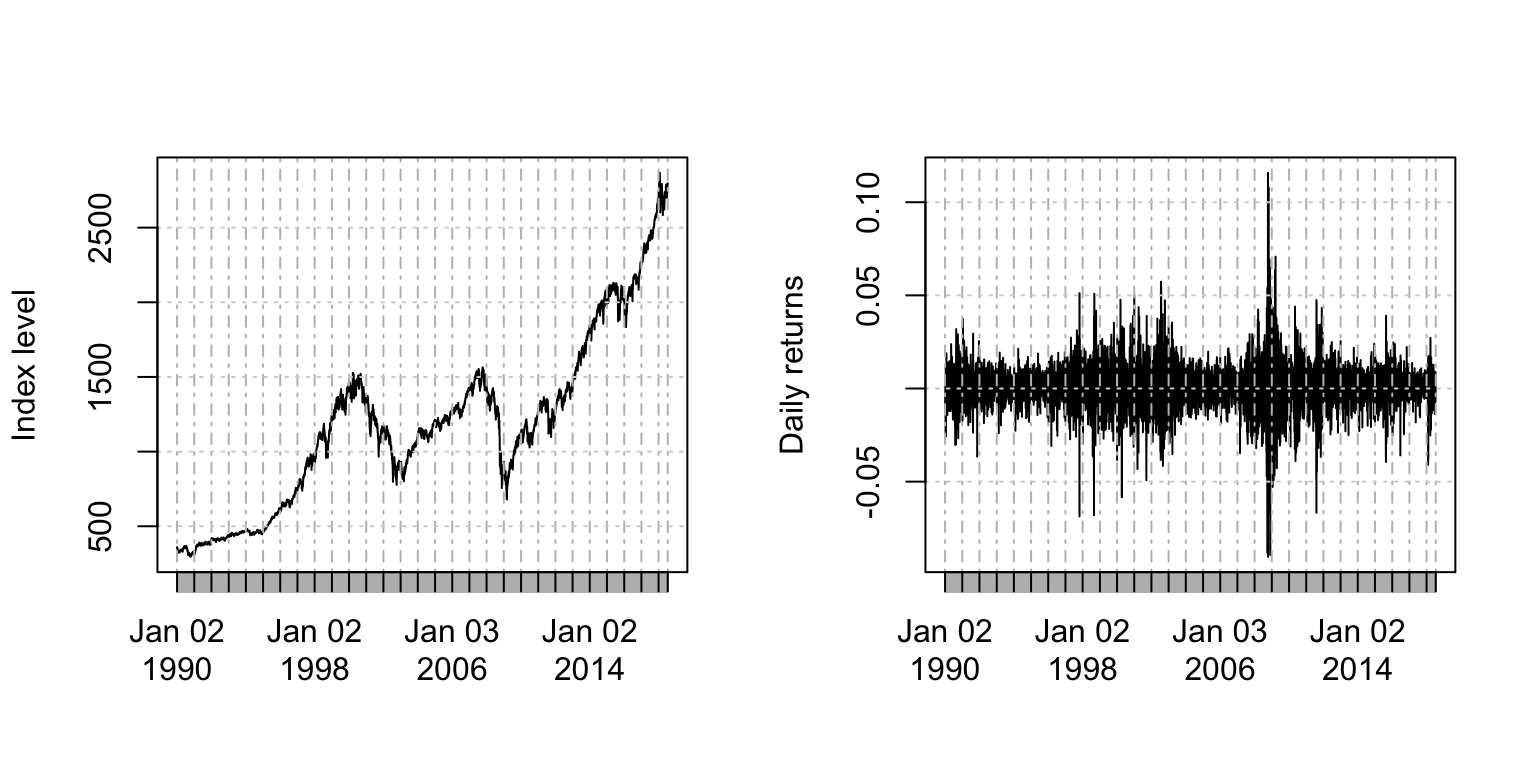
\includegraphics{tts_files/figure-latex/GSPC-1.pdf}

From these graphs, it is clear that the returns are not identically
distributed as the variance seems to vary with time, and clusters with
either high or low volatility can be observed. These characteristics of
financial time series is well known and in the Chapter 5, we will
discuss how the variance of such process can be approximated.
Nevertheless, we compute the empirical autocorrelation function of the
S\&P 500 return to evaluate the degree of ``linear'' dependence between
observations. The graph below presents the empirical autocorrelation.

\begin{Shaded}
\begin{Highlighting}[]
\NormalTok{sp500 =}\StringTok{ }\KeywordTok{na.omit}\NormalTok{(GSPC.ret)}
\KeywordTok{names}\NormalTok{(sp500) =}\StringTok{ }\KeywordTok{paste}\NormalTok{(}\StringTok{"S&P 500 (1990-01-01 - "}\NormalTok{,}\KeywordTok{Sys.Date}\NormalTok{(),}\StringTok{")"}\NormalTok{, }\DataTypeTok{sep =} \StringTok{""}\NormalTok{)}
\KeywordTok{plot}\NormalTok{(}\KeywordTok{ACF}\NormalTok{(sp500))}
\end{Highlighting}
\end{Shaded}

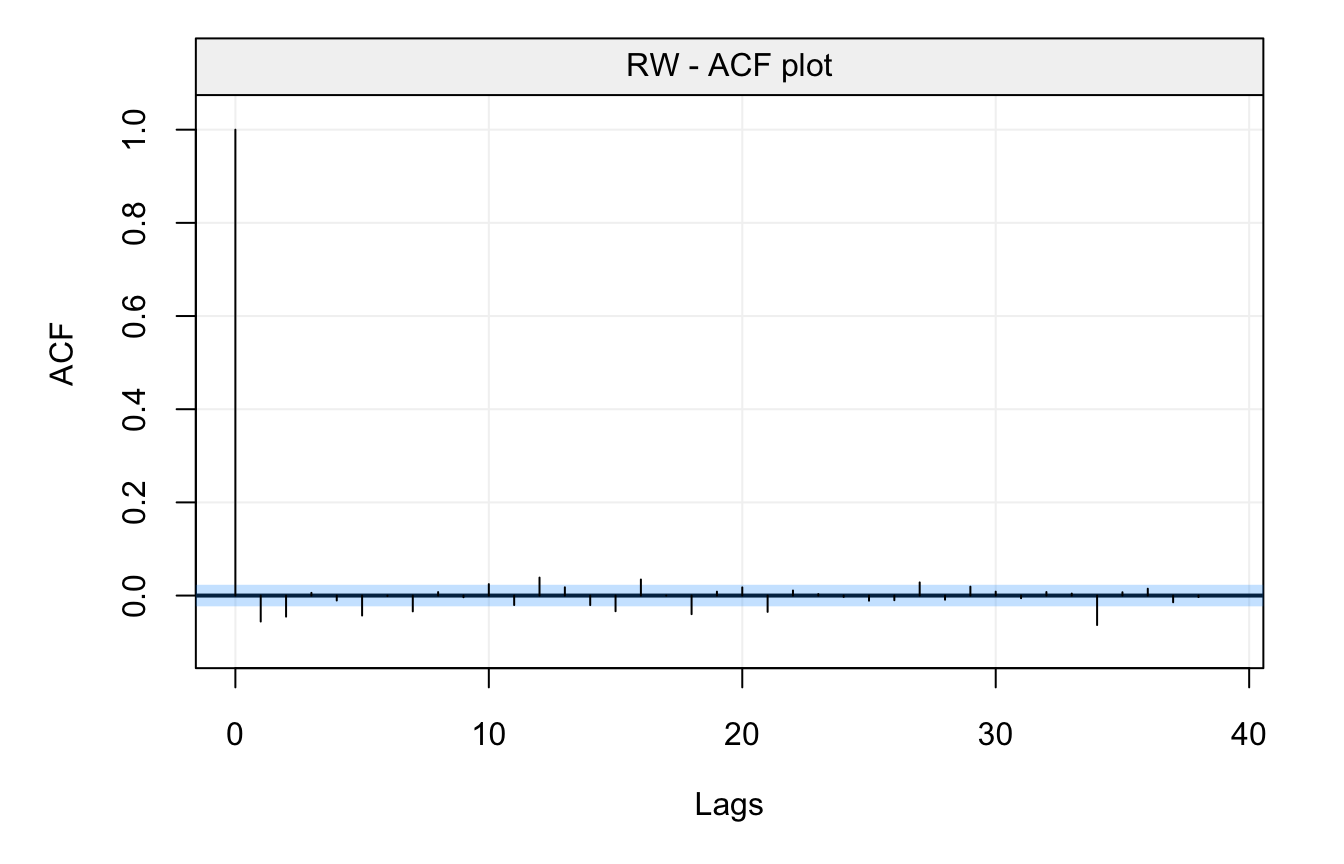
\includegraphics{tts_files/figure-latex/GSPCacf-1.pdf}

As expected, the autocorrelation is small but it might be reasonable to
believe that this sequence is not purely uncorrelated.

Unfortunately, Theorem 1 is based on an asymptotic argument and since
the confidence bands constructed are also asymptotic, there are no
``exact'' tools that can be used in this case. To study the validity of
these results when \(n\) is ``small'' we performed a simulation. In the
latter, we simulated processes following from a Gaussian white noise and
examined the empirical distribution of \(\hat{\rho}(3)\) with different
sample sizes (i.e. \(n\) is set to 5, 10, 30 and 300). Intuitively, the
``quality'' of the approximation provided by Theorem 1 should increase
with the sample size \(n\). The code below performs such a simulation
and compares the empirical distribution of \(\sqrt{n} \hat{\rho}(3)\)
with a normal distribution with mean 0 and variance 1 (its asymptotic
distribution), which is depicted using a red line.

\begin{Shaded}
\begin{Highlighting}[]
\CommentTok{# Number of Monte Carlo replications}
\NormalTok{B =}\StringTok{ }\DecValTok{10000}

\CommentTok{# Define considered lag}
\NormalTok{h =}\StringTok{ }\DecValTok{3}

\CommentTok{# Sample size considered}
\NormalTok{N =}\StringTok{ }\KeywordTok{c}\NormalTok{(}\DecValTok{5}\NormalTok{, }\DecValTok{10}\NormalTok{, }\DecValTok{30}\NormalTok{, }\DecValTok{300}\NormalTok{)}

\CommentTok{# Initialisation}
\NormalTok{result =}\StringTok{ }\KeywordTok{matrix}\NormalTok{(}\OtherTok{NA}\NormalTok{,B,}\KeywordTok{length}\NormalTok{(N))}

\CommentTok{# Set seed}
\KeywordTok{set.seed}\NormalTok{(}\DecValTok{1}\NormalTok{)}

\CommentTok{# Start Monte Carlo}
\ControlFlowTok{for}\NormalTok{ (i }\ControlFlowTok{in} \KeywordTok{seq_len}\NormalTok{(B))\{}
  \ControlFlowTok{for}\NormalTok{ (j }\ControlFlowTok{in} \KeywordTok{seq_along}\NormalTok{(N))\{}
    \CommentTok{# Simluate process}
\NormalTok{    Xt =}\StringTok{ }\KeywordTok{rnorm}\NormalTok{(N[j])}
    
    \CommentTok{# Save autocorrelation at lag h}
\NormalTok{    result[i,j] =}\StringTok{ }\KeywordTok{acf}\NormalTok{(Xt, }\DataTypeTok{plot =} \OtherTok{FALSE}\NormalTok{)}\OperatorTok{$}\NormalTok{acf[h}\OperatorTok{+}\DecValTok{1}\NormalTok{]}
\NormalTok{  \}}
\NormalTok{\}}

\CommentTok{# Plot results}
\KeywordTok{par}\NormalTok{(}\DataTypeTok{mfrow =} \KeywordTok{c}\NormalTok{(}\DecValTok{2}\NormalTok{,}\KeywordTok{length}\NormalTok{(N)}\OperatorTok{/}\DecValTok{2}\NormalTok{))}
\ControlFlowTok{for}\NormalTok{ (i }\ControlFlowTok{in} \KeywordTok{seq_along}\NormalTok{(N))\{}
  \CommentTok{# Estimated empirical distribution}
  \KeywordTok{hist}\NormalTok{(}\KeywordTok{sqrt}\NormalTok{(N[i])}\OperatorTok{*}\NormalTok{result[,i], }\DataTypeTok{col =} \StringTok{"royalblue1"}\NormalTok{, }
       \DataTypeTok{main =} \KeywordTok{paste}\NormalTok{(}\StringTok{"Sample size n ="}\NormalTok{,N[i]), }\DataTypeTok{probability =} \OtherTok{TRUE}\NormalTok{,}
       \DataTypeTok{xlim =} \KeywordTok{c}\NormalTok{(}\OperatorTok{-}\DecValTok{4}\NormalTok{,}\DecValTok{4}\NormalTok{), }\DataTypeTok{xlab =} \StringTok{" "}\NormalTok{)}
  
  \CommentTok{# Asymptotic distribution}
\NormalTok{  xx =}\StringTok{ }\KeywordTok{seq}\NormalTok{(}\DataTypeTok{from =} \DecValTok{-10}\NormalTok{, }\DataTypeTok{to =} \DecValTok{10}\NormalTok{, }\DataTypeTok{length.out =} \DecValTok{10}\OperatorTok{^}\DecValTok{3}\NormalTok{)}
\NormalTok{  yy =}\StringTok{ }\KeywordTok{dnorm}\NormalTok{(xx,}\DecValTok{0}\NormalTok{,}\DecValTok{1}\NormalTok{)}
  \KeywordTok{lines}\NormalTok{(xx,yy, }\DataTypeTok{col =} \StringTok{"red"}\NormalTok{, }\DataTypeTok{lwd =} \DecValTok{2}\NormalTok{)}
\NormalTok{\}}
\end{Highlighting}
\end{Shaded}

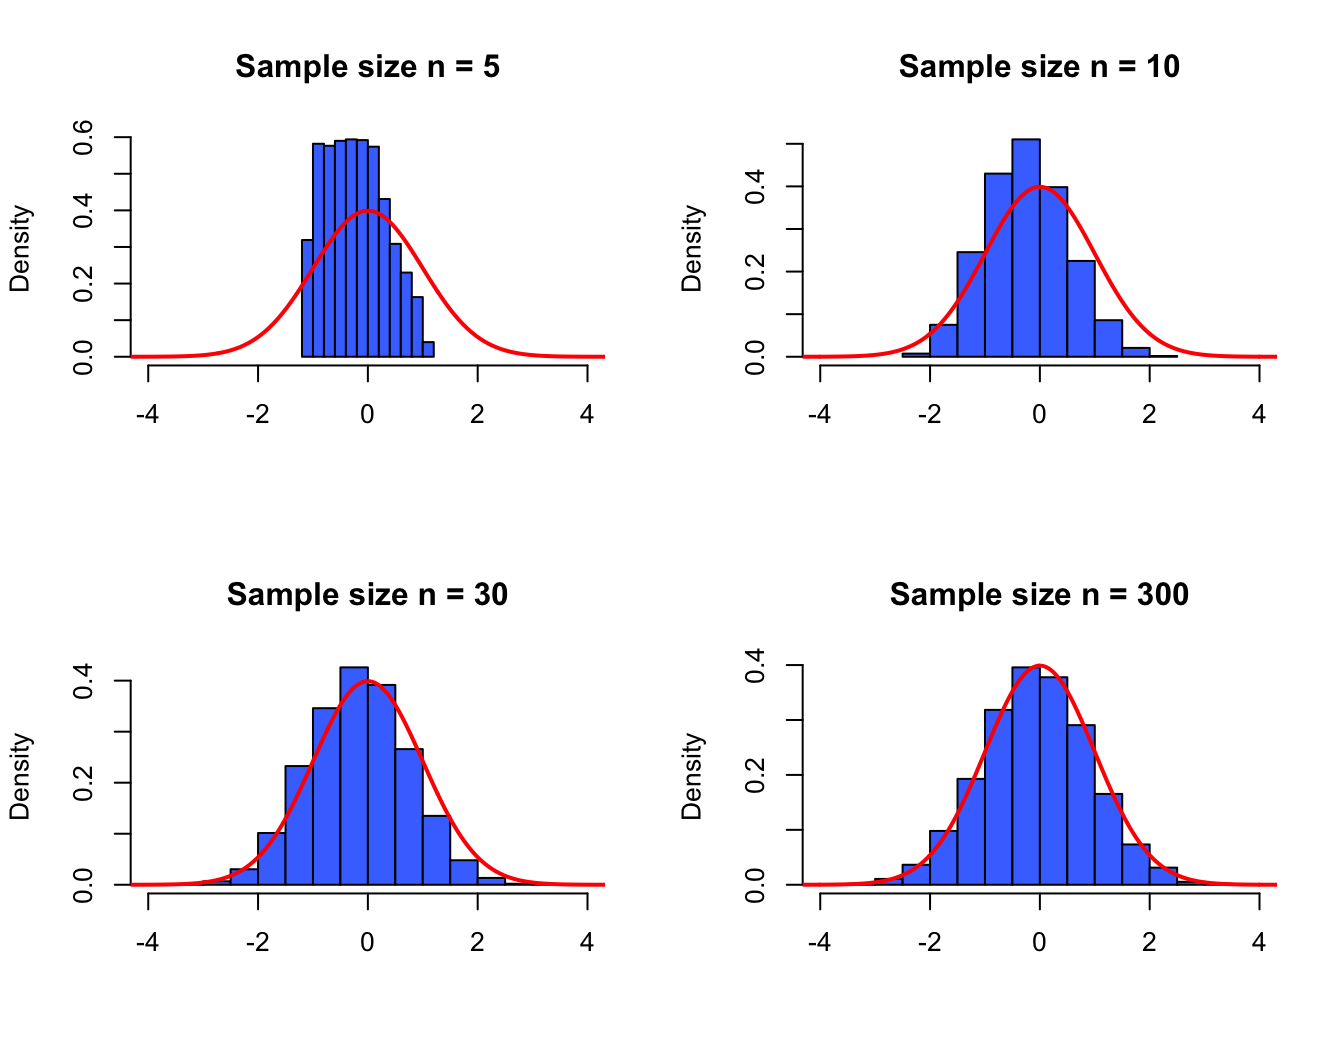
\includegraphics{tts_files/figure-latex/simulationACF-1.pdf}

As expected, it can clearly be observed that the asymptotic
approximation is quite poor when \(n = 5\) but as the sample size
increases the approximation improves and is very close when, for
example, \(n = 300\). This simulation could suggest that Theorem 1
provides a relatively ``close'' approximation of the distribution of
\(\hat{\rho}(h)\).

\hypertarget{robustness-issues}{%
\subsection{Robustness Issues}\label{robustness-issues}}

The data generating process delivers a theoretical autocorrelation
(autocovariance) function that, as explained in the previous section,
can then be estimated through the sample autocorrelation
(autocovariance) functions. However, in practice, the sample is often
issued from a data generating process that is ``close'' to the true one,
meaning that the sample suffers from some form of small contamination.
This contamination is typically represented by a small amount of extreme
observations that are called ``outliers'' that come from a process that
is different from the true data generating process.

The fact that the sample can suffer from outliers implies that the
standard estimation of the autocorrelation (autocovariance) functions
through the sample functions could be highly biased. The standard
estimators presented in the previous section are therefore not
``robust'' and can behave badly when the sample suffers from
contamination. To illustrate this limitation of a classical estimator,
we consider the following two processes:

\[ 
    \begin{aligned}
    X_t &= \phi X_{t-1} + W_t, \;\;\; W_t \sim \mathcal{N}(0,\sigma_w^2),\\
    Y_t &= \begin{cases}
    X_t       & \quad \text{with probability } 1 - \epsilon\\
    U_t  & \quad \text{with probability } \epsilon\\
    \end{cases}, \;\;\; U_t \sim \mathcal{N}(0,\sigma_u^2),
    \end{aligned}
\]

when \(\epsilon\) is ``small'' and \(\sigma_u^2 \gg \sigma_w^2\), the
process \((Y_t)\) can be interpreted as a ``contaminated'' version of
\((X_t)\). The figure below represents one relalization of the processes
\((X_t)\) and \((Y_t)\) using the following setting: \(n = 100\),
\(\sigma_u^2 = 10\), \(\phi = 0,5\), \(\sigma_w^2 = 1\) as well as
\(\alpha = 0.05\).

Next, we consider a simulated example to highlight how the performance
of a ``classical'' autocorrelation can deteriorate if the sample is
contaminated ( i.e.~what is the impact of using \(Y_t\) instead of
\(X_t\), the ``uncontaminated'' process). In this simulation, we will
use the setting presented above and consider \(B = 10^3\) bootstrap
replications.

The boxplots in each figure show how the standard autocorrelation
estimator is centered around the true value (red line) when the sample
is not contaminated (left boxplot) while it is considerably biased when
the sample is contaminated (right boxplot), especially at the smallest
lags. Indeed, it can be seen how the boxplots under contamination are
often close to zero indicating that it does not detect much dependence
in the data although it should. This is a known result in robustness,
more specifically that outliers in the data can break the dependence
structure and make it more difficult for the latter to be detected.

In order to limit this problem, different robust estimators exist for
time series problems which are designed to reduce contamination during
the estimation procedure. Among these estimators, there are a few that
estimate the autocorrelation (autocovariance) functions in a robust
manner. One of these estimators is provided in the \texttt{robacf()}
function in the ``robcor'' package. The following simulated example
shows how it limits bias from contamination. Unlike in the previous
simulation, we shall only consider data issued from the contaminated
model, \(Y_t\), and compare the performance of two estimators
(i.e.~classical and robust autocorrelation estimators):

The robust estimator remains close to the true value represented by the
red line in the boxplots as opposed to the standard estimator. It can
also be observed that to reduce the bias induced by contamination in the
sample, robust estimators pay a certain price in terms of efficiency as
highlighted by the boxplots that show more variability compared to those
of the standard estimator. To assess how much is ``lost'' by the robust
estimator compared to the classical one in terms of efficiency, we
consider one last simulation where we examine the performance of two
estimators on data issued from the uncontaminated model, i.e. \((X_t)\).
Therefore, the only difference between this simulation and the previous
one is the value of \(\alpha\) set equal to \(0\); the code shall thus
be omitted and the results are depicted below:

It can be observed that both estimators provide extremely similar
results, although the robust estimator is slightly more variable.

Next, we consider the issue of robustness on the real data set coming
from the domain of hydrology presented in Section \ref{eda}. This data
concerns monthly precipitation (in mm) over a certain period of time
(1907 to 1972). Let us compare the standard and robust estimators of the
autocorrelation functions:

\begin{Shaded}
\begin{Highlighting}[]
\CommentTok{# TO DO}
\end{Highlighting}
\end{Shaded}

It can be seen that, under certain assumptions (e.g.~linear dependence),
the standard estimator does not detect any significant autocorrelation
between lags since the estimations all lie within the asymptotic
confidence intervals. However, many of the robust estimations lie
outside these confidence intervals at different lags indicating that
there could be dependence within the data. If one were only to rely on
the standard estimator in this case, there may be erroneous conclusions
drawn on this data. Robustness issues therefore need to be considered
for any time series analysis, not only when estimating the
autocorrelation (autocovariance) functions.

Finally, we return to S\&P 500 returns and compare the classical and
robust autocorrelation estimators, which are presented in the figure
below.

\begin{Shaded}
\begin{Highlighting}[]
\CommentTok{# TO DO}
\end{Highlighting}
\end{Shaded}

It can be observed that both estimators are very similar. Nevertheless,
some small discrepancies can be observed. In particular, the robust
estimators seem to indicate an absence of linear dependence while a
slightly different interpretation might be achieved with the classical
estimator.

\hypertarget{joint-stationarity}{%
\section{Joint Stationarity}\label{joint-stationarity}}

The notion of joint stationarity implies that the time series under
investigation is bivariate in nature, e.g. \(\left(X_t \right)\) and
\(\left(Y_t\right)\) are two distinct time series with matching time
points. In order to fulfill bivariate stationarity, both processes must
be considered \emph{weakly stationary} (with constant mean and
autocovariance dependent on lag \(h\)) and there must exist a
cross-covariance function between them, depenent only on lag \(h\). The
ideas discussed next can extended beyond the bivariate case to a general
multivariate setting.

\BeginKnitrBlock{definition}
\protect\hypertarget{def:crosscov}{}{\label{def:crosscov} }The
\textbf{cross-covariance} function of two jointly stationary processes
\(\left\{X_t\right\}\) and \(\left\{Y_t\right\}\) is given by:

\[{\gamma _{XY}}\left( {t + h,t} \right) = \text{cov}\left( {{X_{t+h}},{Y_{t}}} \right) =
      \e{\left( {{X_{t + h}} - {\mu _X}} \right)\left( {{Y_t} - {\mu _Y}} \right)} = {\gamma _{XY}}\left( h \right)\]
\EndKnitrBlock{definition}

Unlike the symmetry found in the autocovariance function of a stationary
process \(\left\{X_t\right\}\), e.g. \(\gamma_X(h) = \gamma_X(-h)\), the
cross-covariance function is only equal when
\(\gamma_{XY}(h) = \gamma_{YX}(-h)\). Notice the switch in indices and
negative lag change.

\BeginKnitrBlock{definition}
\protect\hypertarget{def:crosscorr}{}{\label{def:crosscorr} }The
\emph{cross-correlation} function for two jointly stationary time series
\(\left\{X_t\right\}\) and \(\left\{Y_t\right\}\) can be expressed as:

\[{\rho _{XY}}\left( {t+h,t} \right) = \frac{{{\gamma _{XY}}\left( {t + h,t} \right)}}{{\sqrt {{\gamma _X}\left( 0 \right)} \sqrt {{\gamma _Y}\left( 0 \right)} }} = \frac{{{\gamma _{XY}}\left( h \right)}}{{{\sigma _{{X_{t+h}}}}{\sigma _{{Y_{t}}}}}} = {\rho _{XY}}\left( h \right)\]
\EndKnitrBlock{definition}

Due to the previously discussed symmetry regarding the cross-covariance
function, note that the cross-correlation function also only has
equality when \(\rho_{XY}(h) = \rho_{YX}(-h)\). Thus, note that
\(\rho_{XY}(h) \neq \rho_{XY}(-h)\).

\BeginKnitrBlock{example}
\protect\hypertarget{exm:ccfjs}{}{\label{exm:ccfjs} }Consider two time
series processes given by:

\[\begin{aligned}
     {X_t} &= {W_t} - {W_{t-1}} \\
     {Y_t} &= {W_t} + {W_{t-1}} \\ 
     \end{aligned} \]

where \(W_t \sim WN(0, \sigma^2_W)\).

First check to see if \(\left\{X_t\right\}\) and \(\left\{Y_t\right\}\)
are weakly stationary.

The means of both time series are evident to be \[\begin{aligned}
   E\left[ {{X_t}} \right] &= E\left[ {{Y_t}} \right] = 0 \\
   \end{aligned} \]

The autocovariance for \(\left\{X_t\right\}\) is given as:

\[\begin{aligned}
     {\gamma _X}\left( h \right) &= \text{cov} \left( {{X_{t + h}},{X_t}} \right) \\
     &= \text{cov} \left( {{W_{t + h}} - {W_{t + h - 1}},{W_t} - {W_{t - 1}}} \right) \\
     &= {1_{\left\{ {h = 0} \right\}}}2{\sigma ^2} + {1_{\left\{ {h =  - 1} \right\}}}{-\sigma ^2} + {1_{\left\{ {h = 1} \right\}}}{-\sigma ^2} \\
     &= \begin{cases}
     2\sigma^2_W, &\text{if} h = 0 \\
     -\sigma^2_W, &\text{if} \left|h\right| = 1 \\
     0, &\text{if} \left|h\right| \ge 1 
     \end{cases} 
     \end{aligned} \]

Similarly, the autocovariance for \(\left\{Y_t\right\}\) is calculated
to be:

\[\begin{aligned}
     {\gamma _Y}\left( h \right) &= \text{cov} \left( {{Y_{t + h}},{Y_t}} \right) \\
     &= \text{cov} \left( {{W_{t + h}} + {W_{t + h - 1}},{W_t} + {W_{t - 1}}} \right) \\
     &= {1_{\left\{ {h = 0} \right\}}}2{\sigma ^2} + {1_{\left\{ {h =  - 1} \right\}}}{\sigma ^2} + {1_{\left\{ {h = 1} \right\}}}{\sigma ^2} \\ 
     &= \begin{cases}
     2\sigma^2_W, &\text{if} h = 0 \\
     \sigma^2_W, &\text{if} \left|h\right| = 1 \\
     0, &\text{if} \left|h\right| \ge 1 
     \end{cases} 
     \end{aligned} \]

Next, the cross-covariance for \(\left\{X_t\right\}\) and
\(\left\{Y_t\right\}\):

\[\begin{aligned}
     {\gamma _{XY}}\left( h \right) &= \text{cov} \left( {{X_{t + h}},{Y_t}} \right) \\
     &= \text{cov} \left( {{W_{t + h}} - {W_{t + h - 1}},{W_t} + {W_{t-1}}} \right)  \\ 
     &= \begin{cases}
     0, &\text{if } h = 0 \\
     -\sigma^2_W, &\text{if } h = 1 \\
     \sigma^2_W, &\text{if } h = -1 \\
     0, &\text{if } h \ge 2
     \end{cases}
     \end{aligned}\]

Therefore, based on obtain the weak stationarity for each process and
obtain a cross-covariance function that only depends on the lag \(h\),
the process is joint stationary.

Furthermore, we also have the cross-correlation function as:

\[{\rho _{XY}}\left( {{X_{t + h}},{Y_t}} \right) = \frac{{{\gamma _{XY}}\left( h \right)}}{{{\sigma _X}{\sigma _Y}}} = \frac{{{\gamma _{XY}}\left( h \right)}}{{\sqrt {{\gamma _x}\left( 0 \right)} \sqrt {{\gamma _y}\left( 0 \right)} }} = \frac{{{\gamma _{XY}}\left( h \right)}}{{{\gamma _X}\left( 0 \right)}} = \begin{cases}
    0, &\text{if } h = 0 \\
    -\frac{1}{2}, &\text{if } h = 1 \\
    \frac{1}{2}, &\text{if } h = -1 \\
    0, &\text{if } h \ge 2
    \end{cases}\]
\EndKnitrBlock{example}

\hypertarget{sample-cross-covariance-and-cross-correlation-functions}{%
\subsection{Sample Cross-Covariance and Cross-Correlation
Functions}\label{sample-cross-covariance-and-cross-correlation-functions}}

A natural estimator of the \emph{cross-covariance function} is given by:

\[{{\hat \gamma }_{XY}}\left( h \right) = \frac{1}{T}\sum\limits_{t = 1}^{T - h} {\left( {{X_{t + h}} - \bar X} \right)\left( {{Y_t} - \bar Y} \right)} \]

With this in mind, the ``plug-in'' estimator for the
\emph{cross-correlation function} follows:

\[{{\hat \rho }_{XY}}\left( h \right) = \frac{{{{\hat \gamma }_{XY}}\left( h \right)}}{{\sqrt {{{\hat \gamma }_X}\left( 0 \right)} \sqrt {{{\hat \gamma }_Y}\left( 0 \right)} }}\]

Both of the above estimators are again only symmetric under the above
index and lag transformation.

\hypertarget{portmanteau-test}{%
\section{Portmanteau test}\label{portmanteau-test}}

In this section we give a brief introduction to Portmanteau tests used
in time series analysis. In linear regression, we always need to do a
diagnostic test for residuals after building our model, to check whether
our assumptions are satisfied. If there is no evidence to reject any of
the assumptions, we can say that the linear model we built is adequate.
Otherwise, if the linear model is not adequate, some modifications or
transformations need to be done either for the previous model or for the
data. This rule also applies to time series modeling. In time series
analysis, a wide variety of Portmanteau tests can be used to check the
white noise residuals assumption. We will introduce two of them as
follows, which are based on the ACF of residuals, in order to illustrate
some of ideas behind these kinds of tests.

Dating back to 1970, Box and Pierce proposed the well-known Box-Pierce
test statistic with the following form:

\[Q_{BP} = n\sum_{h =1}^m \hat{\rho}_h^2,\]

where the empirical autocorrelation of residuals at lag \(h\) is defined
as \(\hat{\rho}_h = \frac{\hat{\gamma}(h)}{\hat{\gamma}(0)}\). It is
obvious that under the alternative hypothesis, \(\hat{\rho}_h\) would be
deviate from \(0\), thus a large \(Q_{BP}\) gives us the evidence to
reject the null. Under the null hypothesis that the residuals are white
noise (or equivalently the time series are adequate), it can be shown
that when \(n \to \infty\), we have

\[Q_{BP} \overset{\mathcal{D}}{\to} \chi^2_{m - m^{\prime}},\] where
\(m^{\prime}\) is the number of parameters in the time series model.

\hypertarget{proof}{%
\section{Proof}\label{proof}}

We can write the autocorrelation
\(\bm{\rho} = \left(\rho(1), \rho(2), \dots, \rho(m)\right)^T\), and the
sample autocorrelation
\(\bm{\hat{\rho}} = \left(\hat{\rho}(1), \hat{\rho}(2), \dots, \hat{\rho}(m)\right)^T\).

According to Theorem A.7 in the textbook, under the data generating
process \(X_t = W_t + \mu\), where \(\mu < \infty\) and \((W_t)\) is a
strong white noise process with variance \(\sigma^2\) and finite fourth
moment (i.e. \(\mathbb{E} [W_t^4] < \infty\)), we have
\[\sqrt{n} \left(\mathbf{\hat{\rho}} - \mathbf{\rho}\right) \overset{\mathcal{D}}{\to} V,\]
where the \((p,q)^{th}\) element of \(V\) is
\[v_{pq} = \sum_{u=1}^{\infty}\left[ \rho(u+p) + \rho(u-p) - 2\rho(p)\rho(u) \right] \times \left[ \rho(u+p) + \rho(u-p) - 2\rho(p)\rho(u) \right].\]
And since \(V\) is a positive definite covariance matrix, it follows
that
\[\sqrt{n} V^{-\frac{1}{2}}\left(\mathbf{\hat{\rho}} - \mathbf{\rho}\right) \overset{\mathcal{D}}{\to} \mathcal{N}(\mathbf{0}, I),\]
and also
\[n \left(\mathbf{\hat{\rho}} - \mathbf{\rho}\right)^T V^{-1} \left(\mathbf{\hat{\rho}} - \mathbf{\rho}\right) \overset{\mathcal{D}}{\to} \chi^2_m,\]
Since under the null, \(\mathbf{\rho} = \mathbf{0}\), we have
\[v_{pq} = 
  \begin{cases}
0, \; p \neq q\\
1, \; p = q
\end{cases}
.\]

Thus, it's easy to show that the Box and Pierce test statistic
\[Q_{BP} = n\sum_{h =1}^m \hat{\rho}_h^2,\] under that data generating
process would follow a \(\chi^2\) distribution with \(m\) degree of
freedom.

Before, we supposed that we knew \(\mu\) in our data generating process
exactly, and hence no unknown parameter needed be estimated. Now,
suppose \(\mu\) is unknown and contains \(m^{\prime}\) number of unknown
parameters which we have to estimate. As we know, if our model for
\(\mu\) is correctly specified and those \(m^{\prime}\) unknown
parameters are appropriately estimated, then the underlying model of the
residules of the fitted model would be \(W_t\) as before, but the
\(m^{\prime}\) number of true parameters are replaced by their
estimators. Then \(Q_{BP}\) will still asymptotically follows \(\chi^2\)
but with \(m - m^{\prime}\) degree of freedom.
\(\;\;\;\;\;\;\;\; \blacksquare\)

Then on 1978, Ljung and Box improved Box-Pierce test by standardizing
each \(\hat{\rho}_h\) by its asymptotic variance. The Ljung and Box test
statistic is

\[Q_{LB} = n\sum_{h =1}^m \frac{n+2}{n-h}\hat{\rho}_h^2.\]

It can also be shown that
\(Q_{LB} \overset{\mathcal{D}}{\to} \chi^2_{m - m^{\prime}}\) under the
null. However, compared to \(Q_{BP}\), the distribution of \(Q_{BP}\)
under the null is closer to \(\chi^2_{m - m^{\prime}}\), when \(n\) is
finite.

In the above two examples, the test statistic contains a user specified
parameter \(m\). And for different \(m\), the power of the test would be
different. Thus, much work has gone into either finding an approach for
selecting the optimal \(m\), or finding a new test statistic without
user specified parameters. Moreover, testing white noise can also be
done by checking PACF, or by checking spectral density in the frequency
domain. Therefore, these differing approaches have lead to many
different Portmanteau tests.

Take for an example the following use of a Portmanteau test to show the
distribution of test statistics under the null:

\begin{Shaded}
\begin{Highlighting}[]
\CommentTok{# set seed}
\KeywordTok{set.seed}\NormalTok{(}\DecValTok{1345}\NormalTok{)}

\CommentTok{# Specify models}
\NormalTok{model =}\StringTok{ }\KeywordTok{WN}\NormalTok{(}\DataTypeTok{sigma2 =} \DecValTok{1}\NormalTok{) }\CommentTok{# WN}

\NormalTok{B =}\StringTok{ }\DecValTok{1000} \CommentTok{# number of parametric bootstrap}
\NormalTok{BP.obs =}\StringTok{ }\KeywordTok{rep}\NormalTok{(}\OtherTok{NA}\NormalTok{, B)}
\NormalTok{LB.obs =}\StringTok{ }\KeywordTok{rep}\NormalTok{(}\OtherTok{NA}\NormalTok{, B)}

\ControlFlowTok{for}\NormalTok{ (j }\ControlFlowTok{in} \KeywordTok{seq_len}\NormalTok{(B))\{}
\NormalTok{x =}\StringTok{ }\KeywordTok{gen_gts}\NormalTok{(}\DecValTok{1000}\NormalTok{, model)}
\NormalTok{BP.obs[j] =}\StringTok{ }\KeywordTok{Box.test}\NormalTok{(x, }\DataTypeTok{lag =} \DecValTok{10}\NormalTok{, }\StringTok{"Box-Pierce"}\NormalTok{, }\DataTypeTok{fitdf =} \DecValTok{0}\NormalTok{)}\OperatorTok{$}\NormalTok{statistic}
\NormalTok{LB.obs[j] =}\StringTok{ }\KeywordTok{Box.test}\NormalTok{(x, }\DataTypeTok{lag =} \DecValTok{10}\NormalTok{, }\StringTok{"Ljung-Box"}\NormalTok{, }\DataTypeTok{fitdf =} \DecValTok{0}\NormalTok{)}\OperatorTok{$}\NormalTok{statistic}
\NormalTok{\}}

\NormalTok{sim_results =}\StringTok{ }\KeywordTok{data.frame}\NormalTok{(}\DataTypeTok{sim =} \KeywordTok{c}\NormalTok{(BP.obs, LB.obs),}
\DataTypeTok{simtype =} \KeywordTok{c}\NormalTok{(}\KeywordTok{rep}\NormalTok{(}\StringTok{"Box-Pierce"}\NormalTok{,B), }\KeywordTok{rep}\NormalTok{(}\StringTok{"Ljung-Box"}\NormalTok{,B)))}

\KeywordTok{ggplot}\NormalTok{(}\DataTypeTok{data =}\NormalTok{ sim_results, }\KeywordTok{aes}\NormalTok{(}\DataTypeTok{x =}\NormalTok{ sim)) }\OperatorTok{+}\StringTok{ }
\KeywordTok{geom_histogram}\NormalTok{(}\KeywordTok{aes}\NormalTok{(}\DataTypeTok{y =}\NormalTok{ ..density.., }\DataTypeTok{fill =}\NormalTok{ simtype),}
\DataTypeTok{binwidth =} \DecValTok{1}\NormalTok{, }\DataTypeTok{color =} \StringTok{"black"}\NormalTok{) }\OperatorTok{+}
\KeywordTok{stat_function}\NormalTok{(}\DataTypeTok{fun =}\NormalTok{ dchisq, }\DataTypeTok{args =} \KeywordTok{list}\NormalTok{(}\DataTypeTok{df =} \DecValTok{10}\NormalTok{)) }\OperatorTok{+}
\KeywordTok{facet_wrap}\NormalTok{( }\OperatorTok{~}\StringTok{ }\NormalTok{simtype) }\OperatorTok{+}\StringTok{ }\KeywordTok{ylim}\NormalTok{(}\DecValTok{0}\NormalTok{, }\FloatTok{0.12}\NormalTok{) }\OperatorTok{+}\StringTok{ }
\KeywordTok{labs}\NormalTok{(}\DataTypeTok{fill =} \StringTok{"Statistic"}\NormalTok{, }\DataTypeTok{title =} \StringTok{"Histogram of the Observed Test Statistics"}\NormalTok{,}
\DataTypeTok{y =} \StringTok{"Density"}\NormalTok{, }\DataTypeTok{x =} \StringTok{"Observed Test Statistic"}\NormalTok{)}
\end{Highlighting}
\end{Shaded}

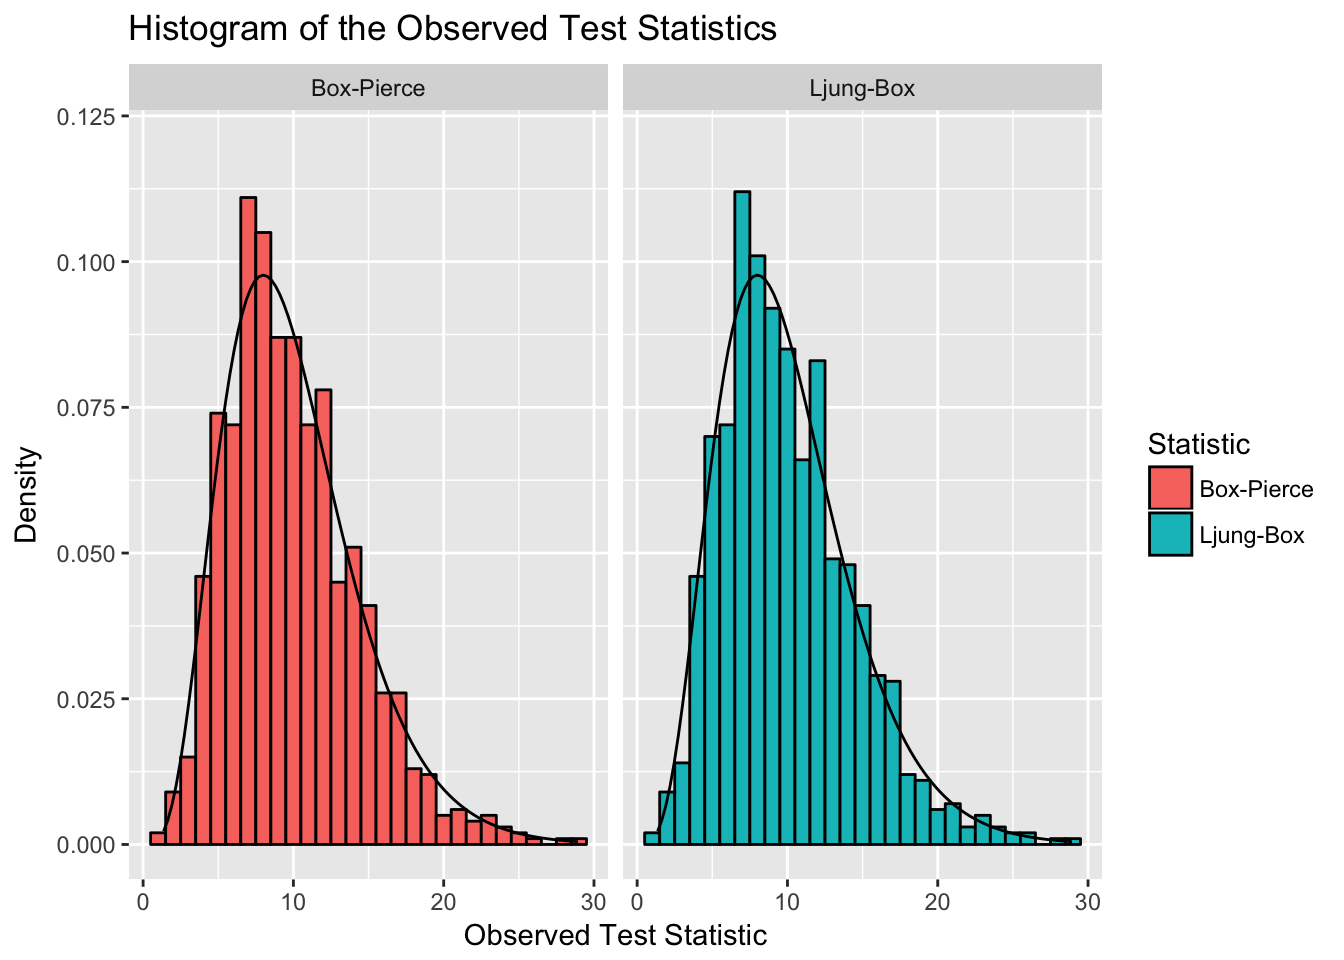
\includegraphics{tts_files/figure-latex/dist_null_portmanteau-1.pdf}

From the histogram, we can see that under the null the distribution of
both BP and LB are close to a Chi-square distribution, but LP is
slightly better.

Consider the following simulation that shows how the test depends on
specified \(m\) and displays the distribution of P-values under
different alternatives.

\begin{Shaded}
\begin{Highlighting}[]
\CommentTok{# Set seed}
\KeywordTok{set.seed}\NormalTok{(}\DecValTok{1234}\NormalTok{)}

\CommentTok{# Specify models}
\NormalTok{model1 =}\StringTok{ }\KeywordTok{WN}\NormalTok{(}\DataTypeTok{sigma2 =} \DecValTok{1}\NormalTok{)                         }\CommentTok{# WN}
\NormalTok{model2 =}\StringTok{ }\KeywordTok{AR}\NormalTok{(}\DataTypeTok{phi =} \FloatTok{0.3}\NormalTok{, }\DataTypeTok{sigma2 =} \DecValTok{1}\NormalTok{)              }\CommentTok{# AR(1)}
\NormalTok{model3 =}\StringTok{ }\KeywordTok{AR}\NormalTok{(}\DataTypeTok{phi =} \KeywordTok{c}\NormalTok{(}\KeywordTok{rep}\NormalTok{(}\DecValTok{0}\NormalTok{,}\DecValTok{9}\NormalTok{), }\FloatTok{0.3}\NormalTok{), }\DataTypeTok{sigma2 =} \DecValTok{1}\NormalTok{) }\CommentTok{# seasonal AR(10)}

\NormalTok{B =}\StringTok{ }\DecValTok{1000} \CommentTok{# number of parametric bootstrap}
\NormalTok{LB.pvalue =}\StringTok{ }\KeywordTok{matrix}\NormalTok{(}\OtherTok{NA}\NormalTok{, }\DataTypeTok{nrow =}\NormalTok{ B, }\DataTypeTok{ncol =} \DecValTok{6}\NormalTok{)}

\ControlFlowTok{for}\NormalTok{ (i }\ControlFlowTok{in} \DecValTok{1}\OperatorTok{:}\DecValTok{3}\NormalTok{)\{}
\ControlFlowTok{for}\NormalTok{ (j }\ControlFlowTok{in} \KeywordTok{seq_len}\NormalTok{(B))\{}
\NormalTok{x =}\StringTok{ }\KeywordTok{gen_gts}\NormalTok{(}\DecValTok{1000}\NormalTok{, }\KeywordTok{get}\NormalTok{(}\KeywordTok{paste0}\NormalTok{(}\StringTok{"model"}\NormalTok{, i)))}
\NormalTok{LB.pvalue[j,}\DecValTok{2}\OperatorTok{*}\NormalTok{i}\DecValTok{-1}\NormalTok{] =}\StringTok{ }\KeywordTok{Box.test}\NormalTok{(x, }\DataTypeTok{lag =} \DecValTok{1}\NormalTok{, }\StringTok{"Ljung-Box"}\NormalTok{, }\DataTypeTok{fitdf =} \DecValTok{0}\NormalTok{)}\OperatorTok{$}\NormalTok{p.value}
\NormalTok{LB.pvalue[j,}\DecValTok{2}\OperatorTok{*}\NormalTok{i] =}\StringTok{ }\KeywordTok{Box.test}\NormalTok{(x, }\DataTypeTok{lag =} \DecValTok{10}\NormalTok{, }\StringTok{"Ljung-Box"}\NormalTok{, }\DataTypeTok{fitdf =} \DecValTok{0}\NormalTok{)}\OperatorTok{$}\NormalTok{p.value}
\NormalTok{\}}
\NormalTok{\}}

\NormalTok{para_}\DecValTok{1}\NormalTok{ =}\StringTok{ }\KeywordTok{data.frame}\NormalTok{(}\DataTypeTok{lag =} \DecValTok{1}\NormalTok{, LB.pvalue[, }\KeywordTok{c}\NormalTok{(}\DecValTok{1}\NormalTok{,}\DecValTok{3}\NormalTok{,}\DecValTok{5}\NormalTok{)])}
\NormalTok{para_}\DecValTok{2}\NormalTok{ =}\StringTok{ }\KeywordTok{data.frame}\NormalTok{(}\DataTypeTok{lag =} \DecValTok{2}\NormalTok{, LB.pvalue[, }\KeywordTok{c}\NormalTok{(}\DecValTok{2}\NormalTok{,}\DecValTok{4}\NormalTok{,}\DecValTok{6}\NormalTok{)])}
\NormalTok{para =}\StringTok{ }\KeywordTok{rbind}\NormalTok{(para_}\DecValTok{1}\NormalTok{, para_}\DecValTok{2}\NormalTok{)}

\KeywordTok{colnames}\NormalTok{(para)[}\DecValTok{2}\OperatorTok{:}\DecValTok{4}\NormalTok{] =}\StringTok{ }\KeywordTok{c}\NormalTok{(}\StringTok{"WN"}\NormalTok{, }\StringTok{"AR(1)"}\NormalTok{, }\StringTok{"Seasonal AR(10)"}\NormalTok{)}

\KeywordTok{library}\NormalTok{(reshape2)}
\end{Highlighting}
\end{Shaded}

\begin{verbatim}
## Warning: package 'reshape2' was built under R version 3.4.3
\end{verbatim}

\begin{Shaded}
\begin{Highlighting}[]
\NormalTok{para.melt =}\StringTok{ }\KeywordTok{melt}\NormalTok{(para, }\DataTypeTok{id.vars =} \StringTok{"lag"}\NormalTok{)}

\KeywordTok{ggplot}\NormalTok{(}\DataTypeTok{data =}\NormalTok{ para.melt, }\KeywordTok{aes}\NormalTok{(}\DataTypeTok{x=}\NormalTok{variable, }\DataTypeTok{y=}\NormalTok{value)) }\OperatorTok{+}\StringTok{ }
\KeywordTok{geom_boxplot}\NormalTok{(}\KeywordTok{aes}\NormalTok{(}\DataTypeTok{fill=}\KeywordTok{factor}\NormalTok{(lag))) }\OperatorTok{+}\StringTok{ }\KeywordTok{facet_wrap}\NormalTok{( }\OperatorTok{~}\StringTok{ }\NormalTok{variable, }\DataTypeTok{scales=}\StringTok{"free"}\NormalTok{) }\OperatorTok{+}
\KeywordTok{ggtitle}\NormalTok{(}\StringTok{"Simulated P-value"}\NormalTok{) }\OperatorTok{+}
\KeywordTok{scale_fill_hue}\NormalTok{(}\DataTypeTok{name=}\StringTok{"Specified m"}\NormalTok{, }\DataTypeTok{breaks =} \KeywordTok{c}\NormalTok{(}\DecValTok{1}\NormalTok{,}\DecValTok{2}\NormalTok{) , }\DataTypeTok{labels =} \KeywordTok{c}\NormalTok{(}\StringTok{"m=1"}\NormalTok{, }\StringTok{"m=10"}\NormalTok{))}
\end{Highlighting}
\end{Shaded}

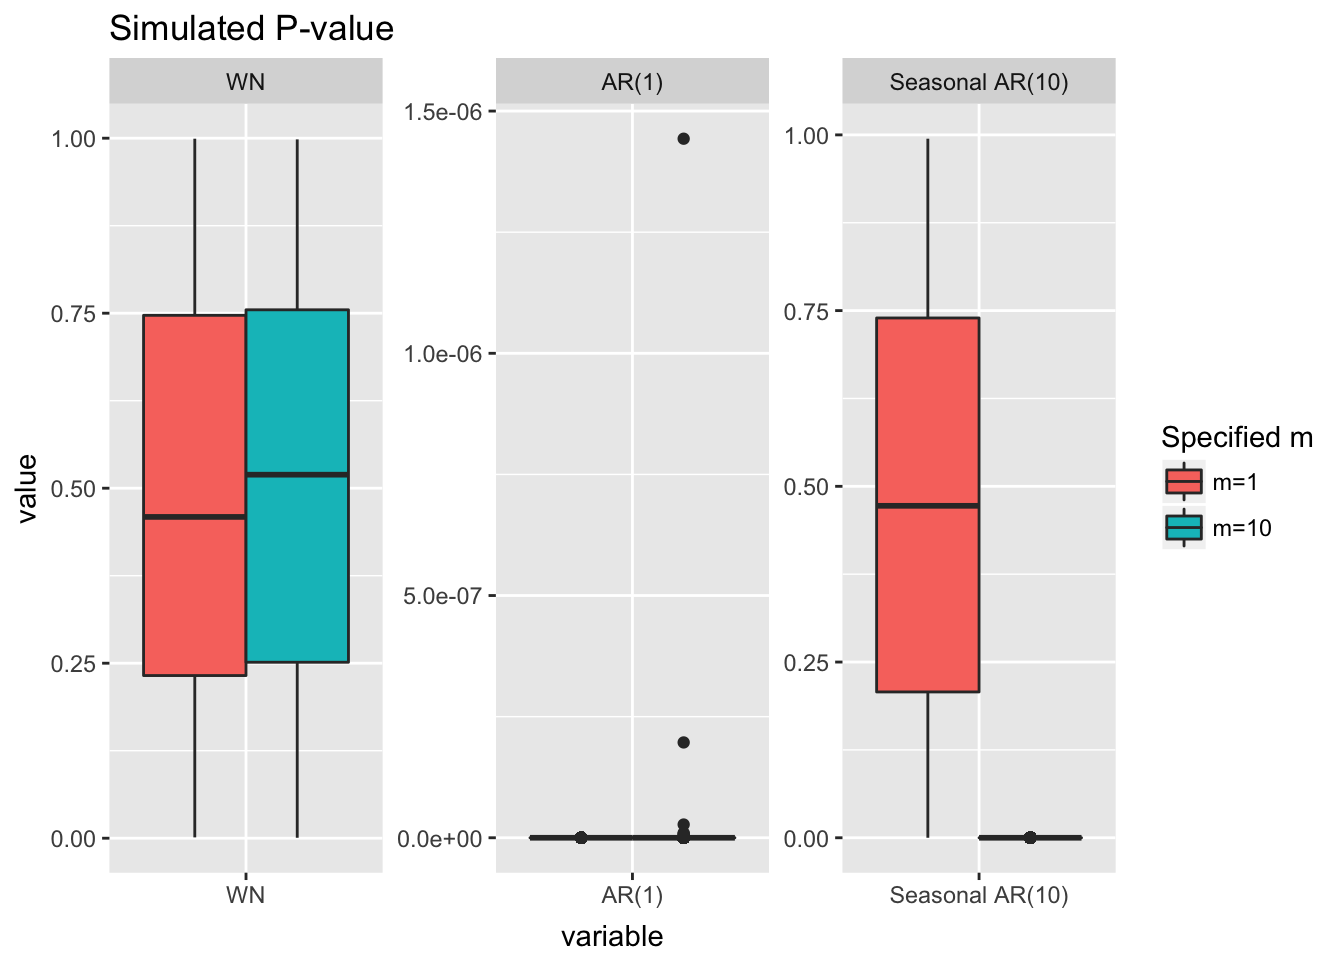
\includegraphics{tts_files/figure-latex/alternatives_port-1.pdf}

\hypertarget{autoregressive-moving-average-models}{%
\chapter{Autoregressive Moving Average
Models}\label{autoregressive-moving-average-models}}

In this chapter we introduce a class of time series models that is
flexible and among the most commonly used to describe stationary time
series. This class is represented by the AutoRegressive Moving Average
(ARMA) models which combine and include the autoregressive and moving
average models seen in the previous chapter, which we first discuss in
further detail before introducing the general ARMA class. The importance
of the latter class of models resides in its flexibility as well as its
capacity of describing (or closely approximating) almost all the
features of a stationary time series. The autoregressive parts of these
models describe how consecutive observations in time influence each
other while the moving average parts capture some possible unobserved
shocks thereby allowing to model different phenomena going from biology
to finance.

To introduce and explain this class of models, this chapter is organized
in the following manner. First of all we will discuss the class of
linear processes of which the ARMA models are part of. We will then
proceed to a detailed description of autoregressive models in which we
review their definition, explain their properties, introduce the main
estimation methods for their parameters and highlight the diagnostic
tools which can help understand if the estimated models appear to be
appropriate or sufficient to well describe the observed time series.
Once this is done, we will then use most of the results given for the
autoregressive models to further desribe and discuss the moving average
models, for which we underline the property of invertibility, and
finally the ARMA models. Indeed, the properties and estimation methods
for the latter class are directly inherited from the discussions on the
autoregressive and moving average models.

\hypertarget{linear-processes}{%
\section{Linear Processes}\label{linear-processes}}

INSERT AN INTRODUCTION TO WHAT LINEAR PROCESSES ARE AND WHY THEY ARE
IMPORTANT

\BeginKnitrBlock{definition}[Linear Process]
\protect\hypertarget{def:lp}{}{\label{def:lp} \iffalse (Linear Process)
\fi{} }A time series, \((X_t)\), is defined to be a linear process if it
can be expressed as a linear combination of white noise by:

\[{X_t} = \mu + \sum\limits_{j =  - \infty }^\infty  {{\psi _j}{W_{t - j}}} \]

where \(W_t \sim WN(0, \sigma^2)\) and
\(\sum\limits_{j = - \infty }^\infty {\left| {{\psi _j}} \right|} < \infty\).
\EndKnitrBlock{definition}

Note, the latter assumption is required to ensure that the series has a
limit. Furthermore, the set of coefficients
\[{\{ {\psi _j}\} _{j =  - \infty , \cdots ,\infty }}\] can be viewed as
linear filter. These coefficients do not have to be all equal nor
symmetric as later examples will show. Generally, the properties of a
linear process related to mean and variance are given by:

\[\begin{aligned}
\mu_{X} &= \mu \\
\gamma_{X}(h) &= \sigma _W^2\sum\limits_{j =  - \infty }^\infty  {{\psi _j}{\psi _{h + j}}}
\end{aligned}\]

The latter is derived from

\[\begin{aligned}
  \gamma \left( h \right) &= Cov\left( {{x_t},{x_{t + h}}} \right) \\
   &= Cov\left( {\mu  + \sum\limits_{j =  - \infty }^\infty  {{\psi _j}{w_{t - j}}} ,\mu  + \sum\limits_{j =  - \infty }^\infty  {{\psi _j}{w_{t + h - j}}} } \right) \\
   &= Cov\left( {\sum\limits_{j =  - \infty }^\infty  {{\psi _j}{w_{t - j}}} ,\sum\limits_{j =  - \infty }^\infty  {{\psi _j}{w_{t + h - j}}} } \right) \\
   &= \sum\limits_{j =  - \infty }^\infty  {{\psi _j}{\psi _{j + h}}Cov\left( {{w_{t - j}},{w_{t - j}}} \right)}  \\
   &= \sigma _w^2\sum\limits_{j =  - \infty }^\infty  {{\psi _j}{\psi _{j + h}}}  \\ 
\end{aligned} \]

Within the above derivation, the key is to realize that
\(Cov\left( {{w_{t - j}},{w_{t + h - j}}} \right) = 0\) if
\(t - j \ne t + h - j\).

Lastly, one of the better formalities of a linear process is that it is
able to be represented in a simplified form under the \textbf{backshift
operator}:

\[{X_t} = \psi \left( B \right){W_t}\]

\BeginKnitrBlock{example}[Linear Process of White Noise]
\protect\hypertarget{exm:lpwn}{}{\label{exm:lpwn} \iffalse (Linear Process
of White Noise) \fi{} } The white noise process \(\left\{X_t\right\}\),
defined in \ref{wn}, can be expressed as a linear process under:

\[\psi _j = \begin{cases}
      1 , &\mbox{ if } j = 0\\
      0 , &\mbox{ if } |j| \ge 1
\end{cases}.\]

and \(\mu = 0\).

Therefore, \(X_t = W_t\), where \(W_t \sim WN(0, \sigma^2_W)\)
\EndKnitrBlock{example}

\BeginKnitrBlock{example}[Linear Process of Moving Average Order 1]
\protect\hypertarget{exm:lpma1}{}{\label{exm:lpma1} \iffalse (Linear Process
of Moving Average Order 1) \fi{} } Similarly, consider
\(\left\{X_t\right\}\) to be a MA(1) process, given by \ref{ma1}. The
process can be expressed linearly under:

\[\psi _j = \begin{cases}
      1, &\mbox{ if } j = 0\\
      \theta , &\mbox{ if } j = 1 \\
      0, &\mbox{ if } j \ge 2
\end{cases}.\]

and \(\mu = 0\).

Thus, we have: \(X_t = W_t + \theta W_{t-1}\)
\EndKnitrBlock{example}

\BeginKnitrBlock{example}[Linear Process and Symmetric Moving Average]
\protect\hypertarget{exm:lpsma}{}{\label{exm:lpsma} \iffalse (Linear Process
and Symmetric Moving Average) \fi{} } Consider a symmetric moving
average given by:

\[{X_t} = \frac{1}{{2q + 1}}\sum\limits_{j =  - q}^q {{W_{t + j}}} \]

Thus, \(\left\{X_t\right\}\) is defined for \(q + 1 \le t \le n-q\). The
above process would be a linear process since:

\[\psi _j = \begin{cases}
      \frac{1}{{2q + 1}} , &\mbox{ if } -q \le j \le q\\
      0 , &\mbox{ if } |j| > q
\end{cases}.\]

and \(\mu = 0\).

In practice, if \(q = 1\), we would have:

\[{X_t} = \frac{1}{3}\left( {{W_{t - 1}} + {W_t} + {W_{t + 1}}} \right)\]
\EndKnitrBlock{example}

\BeginKnitrBlock{example}[Linear Process of Autoregressive Process of Order 1]
\protect\hypertarget{exm:lpar1}{}{\label{exm:lpar1} \iffalse (Linear Process
of Autoregressive Process of Order 1) \fi{} }A more intensive
application of a linear process is \(\left\{X_t\right\}\) as an AR1
process, defined in \ref{ar1}. The intensity comes from the necessity to
define the weights with respect to the time lag.

\[\psi _j = \begin{cases}
      \phi^j , &\mbox{ if } j \ge 0\\
      0 , &\mbox{ if } j < 0
\end{cases}.\]

and \(\mu = 0\).

Under the condition that \(\left| \phi \right| < 1\) the process can be
considered to be the traditional \(X_t = \phi X_{t-1} + W_t\).
Furthermore, the process can also be considered to be an MA(\(\infty\))!
\EndKnitrBlock{example}

\hypertarget{linear-operators}{%
\section{Linear Operators}\label{linear-operators}}

\hypertarget{autoregressive-models-arp}{%
\section{Autoregressive Models
(AR(p))}\label{autoregressive-models-arp}}

The class of autoregressive models is based on the idea that previous
values in the time series are needed to explain current values in the
series. For this class of models, we assume that the \(p\) previous
observations are needed for this purpose and we therefore denote this
class as AR(\(p\)). In the previous chapter, the model we introduced was
an AR(1) in which only the immediately previous observation is needed to
explain the following one and therefore represents a particular model
which is part of the more general class of AR(p) models.

\BeginKnitrBlock{definition}
\protect\hypertarget{def:ar_p}{}{(\#def:ar\_p) }The AR(p) models can be
formally represented as follows
\[{X_t} = {\phi_1}{Y_{t - 1}} + ... + {\phi_p}{X_{t - p}} + {W_t},\]
where \(\phi_p \neq 0\) and \(W_t\) is a (Gaussian) white noise process
with variance \(\sigma^2\).
\EndKnitrBlock{definition}

In general, we will assume that the expectation of the process
\(({X_t})\), as well as that of the following ones in this chapter, is
zero. The reason for this simplification is that if
\(\mathbb{E} [ X_t ] = \mu\), we can define an AR process \emph{around}
\(\mu\) as follows:

\[X_t - \mu = \sum_{i = 1}^p \left(\phi_i X_{t-i} - \mu \right) + W_t,\]

which is equivalent to

\[X_t  = \mu^{\star} +  \sum_{i = 1}^p \phi_i X_{t-i}  + W_t,\]

where \(\mu^{\star} = \mu (1 - \sum_{i = 1}^p \phi_i)\). Therefore, to
simplify the notation we will generally consider only zero mean
processes, since adding means (as well as other deterministic trends) is
easy.

A useful way of representing AR processes is through the backshift
operator introduced in the previous section and is as follows

\[\begin{aligned}
  {X_t} &= {\phi_1}{X_{t - 1}} + ... + {\phi_p}{y_{t - p}} + {w_t} \\
   &= {\phi_1}B{X_t} + ... + {\phi_p}B^p{X_t} + {W_t} \\
   &= ({\phi_1}B + ... + {\phi_p}B^p){X_t} + {W_t} \\ 
\end{aligned},\]

which finally yields

\[(1 - {\phi _1}B - ... - {\phi_p}B^p){X_t} = {W_t},\]

which, in abbreviated form, can be expressed as

\[\phi(B){X_t} = W_t.\]

We will see that \(\phi(B)\) is important to establish the stationarity
of these processes and is called the \emph{autoregressive} operator.
Moreover, this quantity is closely related to another important property
of AR processes called \emph{causality}. Before formally defining this
new property, we consider the following example, which provides an
intuitive illustration of its importance.

\textbf{Example:} Consider a classical AR(1) model with \(|\phi| > 1\).
Such a model could be expressed as

\[X_t = \phi^{-1} X_{t+1} - \phi^{-1} W_t = \phi^{-k} X_{t+k} - \sum_{i = 1}^{k-1} \phi^{-i} W_{t+i}.\]

Since \(|\phi| > 1\), we obtain

\[X_t = - \sum_{i = 1}^{\infty} \phi^{-j} W_{t-j},\]

which is a linear process and therefore is stationary. Unfortunately,
such a model is useless because we need the future to predict the future
and such processes are called non-causal.

\hypertarget{properties-of-arp-models}{%
\subsection{Properties of AR(p) models}\label{properties-of-arp-models}}

In this section we will describe the main property of the AR(p) model
which has already been introduced in the previous paragraphs and
therefore let us now introduce the property of causality in a more
formal manner.

\textbf{Definition:} An AR(p) model is \emph{causal}, if the time series
\(\{ X_t \}_{-\infty}^{\infty}\) can be written as a one-sided linear
process: \begin{equation}
    X_t = \sum_{j = 0}^{\infty} \psi_j W_{t-j} = \frac{1}{\phi(B)} W_t = \psi(B) W_t,
\label{eq:causal}
\end{equation} where \(\phi(B) = \sum_{j = 0}^{\infty} \phi_j B^j\), and
\(\sum_{j=0}^{\infty}|\phi_j| < \infty\); we set \(\phi_0 = 1\).

As discussed earlier this condition implies that only the past values of
the time series can explain the future values of it, and not viceversa.
However, it might be difficult and not obvious to show the causality of
an AR(p) process by using the above definitions directly, thus the
following properties are useful in practice.

\textbf{Property: Causality} If an AR(p) model is causal, then the
coefficients of the one-sided linear process given in (\eqref{eq:causal})
can be obtained by solving \begin{equation*}
    \psi(z) = \frac{1}{\sum_{j=0}^{\infty} \phi_j z^j} = \frac{1}{\phi(z)}, \mbox{ } |z| \leq 1.
\end{equation*}

It can be seen how there is no solution to the above equation if
\(\phi(z) = 0\) and therefore an AR(p) is causal if and only if
\(\phi(z) \neq 0\). A condition for this to be respected is for the
roots of \(\phi(z) = 0\) to lie outside the unit circle.

\hypertarget{estimation-of-arp-models}{%
\section{Estimation of AR(p) models}\label{estimation-of-arp-models}}

Given the above defined properties of the AR(p) models, we will now
discuss how these models can be estimated, more specifically how the
\(p+1\) parameters can be obtained from an observed time series. Indeed,
a reliable estimation of these models is necessary in order to intepret
and describe different natural phenomena and/or forecast possible future
values of the time series.

A first approach builds upon the earlier definition of the AR(p) as
being a linear process. Recall that \begin{equation}
    X_t = \sum_{j = 1}^{p} \phi_j X_{t-j}
\end{equation} which delivers the following autocovariance function
\begin{equation}
    \gamma(h) = cov(X_{t+h}, X_t) = cov(\sum_{j = 1}^{p} \phi_j X_{t-j}, X_t) = \sum_{j = 1}^{p} \phi_j \gamma(h-j), \mbox{ } h \geq 0.
\end{equation} Rearranging the above expressions we obtain the following
general equations \begin{equation}
    \gamma(h) - \sum_{j = 1}^{p} \phi_j \gamma(h-j) = 0, \mbox{ } h \geq 1
\end{equation} and, recalling that \(\gamma(h) = \gamma(-h)\),
\begin{equation}
    \gamma(0) - \sum_{j = 1}^{p} \phi_j \gamma(j) = \sigma_w^2.
\end{equation} We can now define the Yule-Walker equations.

\textbf{Definition:} The Yule-Walker equations are given by
\begin{equation}
    \gamma(h) = \phi_1 \gamma(h-1) + ... + \phi_p \gamma(h-p), \mbox{ } h = 1,...,p
\end{equation} and \begin{equation}
    \sigma_w^2 = \gamma(0) - \phi_1 \gamma(1) - ... - \phi_p \gamma(p).
\end{equation} which in matrix notation can be defined as follows
\begin{equation}
    \Gamma_p \mathbf{\phi} = \mathbf{\gamma}_p \text{and} \sigma_w^2 = \gamma(0) - \mathbf{\phi}'\mathbf{\gamma}_p
\end{equation} where \(\Gamma_p\) is the \(p\times p\) matrix containing
the autocovariances \(\gamma(k-j), j,k = 1, ...,p\) while
\(\mathbf{\phi} = (\phi_1,...,\phi_p)'\) and
\(\mathbf{\gamma}_p = (\gamma(1),...,\gamma(p))'\) are \(p\times 1\)
vectors.

Considering the Yule-Walker equations, it is possible to use a method of
moments approach and simply replace the theoretical quantities given in
the previous definition with their empirical (estimated) counterparts
that we saw in the previous chapter. This gives us the following
Yule-Walker estimators \begin{equation}
    \hat{\mathbf{\phi}} = \hat{\Gamma}_p^{-1}\hat{\mathbf{\gamma}}_p \text{and} \hat{\sigma}_w^2 = \hat{\gamma}(0) - \hat{\mathbf{\gamma}}_p'\hat{\Gamma}_p^{-1}\hat{\mathbf{\gamma}}_p
\end{equation}

These estimators have the following asymptotic properties.

\textbf{Property: Consistency and Asymptotic Normality of Yule-Walker
estimators} The Yule-Walker estimators for a causal AR(p) model have the
following asymptotic properties:

\begin{equation*}
\sqrt{T}(\hat{\mathbf{\phi}}- \mathbf{\phi}) \xrightarrow{\mathcal{D}} \mathcal{N}(\mathbf{0},\sigma_w^2\Gamma_p^{-1}) \text{and} \hat{\sigma}_w^2 \xrightarrow{\mathcal{P}} \sigma_w^2 .
\end{equation*}

Therefore the Yule-Walker estimators have an asymptotically normal
distribution and the estimator of the innovation variance is consistent.
Moreover, these estimators are also optimal for AR(p) models, meaning
that they are also efficient. However, there exists another method which
allows to achieve this efficiency also for general ARMA models and this
is the maximum likelihood method. Considering an AR(1) model as an
example, and assuming without loss of generality that the expectation is
zero, we have the following representation of the AR(1) model
\begin{equation*}
X_t = \phi X_{t-1} + w_t
\end{equation*} where \(|\phi|<1\) and
\(w_t \overset{iid}{\sim} \mathcal{N}(0,\sigma_w^2)\). Supposing we have
observations issued from this model \((x_t)_{t=1,...,T}\), then the
likelihood function for this setting is given by \begin{equation*}
L(\phi,\sigma_w^2) = f(\phi,\sigma_w^2|x_1,...,x_T)
\end{equation*} which, for an AR(1) model, can be rewritten as follows
\begin{equation*}
L(\phi,\sigma_w^2) = f(x_1)f(x_2|x_1)\cdot \cdot \cdot f(x_T|x_{T-1}).
\end{equation*} If we define \(\Omega_t^p\) as the information contained
in the previous \(p\) observations to time \(t\), the above can be
generalized for an AR(p) model as follows \begin{equation*}
L(\phi,\sigma_w^2) = f(x_1,...,x_p)f(x_{p+1}|\Omega_{p+1}^p)\cdot \cdot \cdot f(x_T|\Omega_{T-1}^p)
\end{equation*} where \(f(x_1,...,x_p)\) is the joint probability
distribution of the first \(p\) observations. A discussion on how to
find \(f(x_1,...,x_p)\) will be presented in the following paragraphs
based on the approach to find \(f(x_1)\) in the AR(1) likelihood. Going
back to the latter, we know that
\(x_t|x_{t-1} \sim \mathcal{N}(\phi x_{t-1},\sigma_w^2)\) and therefore
we have that \begin{equation*}
f(x_t|x_{t-1}) = f_w(x_t - \phi x_{t-1})
\end{equation*} where \(f_w(\cdot)\) is the distribution of \(w_t\).
This rearranges the likelihood function as follows \begin{equation*}
L(\phi,\sigma_w^2) = f(x_1)\prod_{t=2}^T f_w(x_t - \phi x_{t-1})
\end{equation*} where \(f(x_1)\) can be found through the causal
representation \begin{equation*}
x_1 = \sum_{j=0}^{\infty} \phi^j w_{1-j} 
\end{equation*} which implies that \(x_1\) follows a normal distribution
with zero expectation and a variance given by
\(\frac{\sigma_w^2}{(1-\phi^2)}\). Based on this, the likelihood
function of an AR(1) finally becomes \begin{equation*}
L(\phi,\sigma_w^2) = (2\pi \sigma_w^2)^{-\frac{n}{2}} (1 - \phi)^2 \exp \left(-\frac{S(\phi)}{2 \sigma_w^2}\right)
\end{equation*} with
\(S(\phi) = (1-\phi)^2 x_1^2 + \sum_{t=2}^T (x_t -\phi x_{t-1})^2\).
Once the derivative of the logarithm of the likelihood is taken, the
minimization of the negative of this function is usually done
numerically. However, if we condition on the initial values, the AR(p)
models are linear and, for example, we can then define the conditional
likelihood of an AR(1) as \begin{equation*}
L(\phi,\sigma_w^2|x_1) = (2\pi \sigma_w^2)^{-\frac{n-1}{2}} \exp \left(-\frac{S_c(\phi)}{2 \sigma_w^2}\right)
\end{equation*} where \begin{equation*}
S_c(\phi) = \sum_{t=2}^T (x_t -\phi x_{t-1})^2 .
\end{equation*} The latter is called the conditional sum of squares and
\(\phi\) can be estimated as a straightforward linear regression
problem. Once an estimate \(\hat{\phi}\) is obtained, this can be used
to obtain the conditional maximum likelihood estimate of \(\sigma_w^2\)
\begin{equation*}
\hat{\sigma}_w^2 = \frac{S_c(\hat{\phi})}{(n-1)} .
\end{equation*}

The estimation methods presented so far are standard ones for these kind
of models. Nevertheless, if the data suffers from some form of
contamination, these methods can become highly biased. For this reason,
some robust estimators are available to limit this problematic if there
are indeed outliers in the observed time series. A first solution is
given by the estimator proposed in Kunsch (1984) who underlines that the
MLE score function of an AR(p) is given by \begin{equation*}
 \kappa(\mathbf{\theta}|x_j,...x_{j+p}) = \frac{\partial}{\partial \mathbf{\theta}} (x_{j+p} - \sum_{k=1}^p \phi_k x_{j+p-k})^2
\end{equation*} where \(\theta\) is the parameter vector containing, in
the case of an AR(1) model, the two parameters \(\phi\) and
\(\sigma_w^2\) (i.e.\(\theta = [\phi \,\, \sigma_w^2]\)). This delivers
the estimating equation \begin{equation*}
\sum_{j=1}^{n-p} \kappa (\hat{\mathbf{\theta}}|x_j,...x_{j+p}) = 0 .
\end{equation*} The score function \(\kappa(\cdot)\) is clearly not
bounded, in the sense that if we arbitrarily move a value of \((x_t)\)
to infinity then the score function also goes to infinity thereby
delivering a biased estimation procedure. To avoid that outlying
observations bias the estimation excessively, a bounded score function
can be used to deliver an M-estimator given by \begin{equation*}
\sum_{j=1}^{n-p} \psi (\hat{\mathbf{\theta}}|x_j,...x_{j+p}) = 0,
\end{equation*} where \(\psi(\cdot)\) is a function of bounded
variation. When conditioning on the first \(p\) observations, this
problem can be brought back to a linear regression problem which can be
applied in a robust manner using the robust regression tools available
in \emph{R} such as \texttt{rlm(...)} or \texttt{lmrob(...)}. However,
another available tool in \emph{R} which can applied directly without
conditioning also for general ARMA models is the \texttt{gmwm(...)}
function which, by specifying the option \texttt{robust\ =\ TRUE}. This
function makes use of a quantity called the wavelet variance (denoted as
\(\nu\)) which is estimated robustly and then used to retrieve the
parameters \(\theta\) of the time series model. The robust estimate is
obtained by solving the following minimization problem \begin{equation*}
\hat{\boldsymbol{\theta}} = \underset{\boldsymbol{\theta} \in \boldsymbol{\Theta}}{\text{argmin}} (\hat{\boldsymbol{\nu}} - \boldsymbol{\nu}(\boldsymbol{\theta}))^T\boldsymbol{\Omega}(\hat{\boldsymbol{\nu}} - \boldsymbol{\nu}({\boldsymbol{\theta}})),
\end{equation*} where \(\hat{\nu}\) is the robustly estimated wavelet
variance, \(\nu{\theta}\) is the theoretical wavelet variance and
\(\Omega\) is positive definite weighting matrix. Below we show some
simulation studies where we present the results of the above estimation
procedures in absence and in presence of contamination in the data.

In particular, we simulate three different processes \(X_t, Y_t, Z_t\)
from \[X_t = 0.5 X_{t-1} - 0.25 X_{t-2} + W_t\] with
\(W_t \sim WN(0, 1)\). Within two of the processes, we apply either a
process-wise contamination or a pointwise contamination. The process
wise contamination, \(Y_t\), has a portion of the original process,
\(X_t\) replaced with concurrent samples from
\[U_t = 0.90 U_{t-1} - 0.40 U_{t-2} + V_t\], where \(V_t \sim WN(0, 9)\)
whereas the point-wise contaimination, \(Z_t\), has points selected at
random from \(X_t\) and replaced with \(N_t \sim WN(0, 9)\).

\begin{Shaded}
\begin{Highlighting}[]
\NormalTok{n         =}\StringTok{ }\DecValTok{1000}           \CommentTok{# Sample Size}
\NormalTok{gamma     =}\StringTok{ }\FloatTok{0.05}           \CommentTok{# Level of contamination}
\NormalTok{dispersal =}\StringTok{ }\KeywordTok{round}\NormalTok{(gamma}\OperatorTok{*}\NormalTok{n) }\CommentTok{# Amount of samples contaminated}

\KeywordTok{set.seed}\NormalTok{(}\DecValTok{19}\NormalTok{)               }\CommentTok{# Set seed for reproducibility}

\CommentTok{# Generate data!}
\NormalTok{Xt =}\StringTok{ }\KeywordTok{gen_gts}\NormalTok{(n, }\KeywordTok{AR}\NormalTok{(}\DataTypeTok{phi =} \KeywordTok{c}\NormalTok{(}\FloatTok{0.5}\NormalTok{,}\FloatTok{0.25}\NormalTok{), }\DataTypeTok{sigma2 =} \DecValTok{1}\NormalTok{))}
\NormalTok{Yt =}\StringTok{ }\KeywordTok{gen_gts}\NormalTok{(n, }\KeywordTok{AR}\NormalTok{(}\DataTypeTok{phi =} \KeywordTok{c}\NormalTok{(}\FloatTok{0.5}\NormalTok{,}\FloatTok{0.25}\NormalTok{), }\DataTypeTok{sigma2 =} \DecValTok{1}\NormalTok{))}
\NormalTok{Zt =}\StringTok{ }\KeywordTok{gen_gts}\NormalTok{(n, }\KeywordTok{AR}\NormalTok{(}\DataTypeTok{phi =} \KeywordTok{c}\NormalTok{(}\FloatTok{0.5}\NormalTok{,}\FloatTok{0.25}\NormalTok{), }\DataTypeTok{sigma2 =} \DecValTok{1}\NormalTok{))}

\CommentTok{# Contaminate a portion of Y_t with a process}
\NormalTok{Yt[}\DecValTok{101}\OperatorTok{:}\DecValTok{135}\NormalTok{,] =}\StringTok{ }\KeywordTok{gen_gts}\NormalTok{(}\DecValTok{35}\NormalTok{, }\KeywordTok{AR}\NormalTok{(}\DataTypeTok{phi =} \KeywordTok{c}\NormalTok{(}\FloatTok{0.9}\NormalTok{,}\OperatorTok{-}\FloatTok{0.4}\NormalTok{), }\DataTypeTok{sigma2 =} \DecValTok{9}\NormalTok{))}

\CommentTok{# Contaminate at random Z_t with noise}
\NormalTok{Zt[}\KeywordTok{sample}\NormalTok{(n, dispersal, }\DataTypeTok{replace =} \OtherTok{FALSE}\NormalTok{),] =}\StringTok{ }\KeywordTok{gen_gts}\NormalTok{(dispersal, }\KeywordTok{WN}\NormalTok{(}\DataTypeTok{sigma2 =} \DecValTok{9}\NormalTok{))}
\end{Highlighting}
\end{Shaded}

\begin{figure}

{\centering 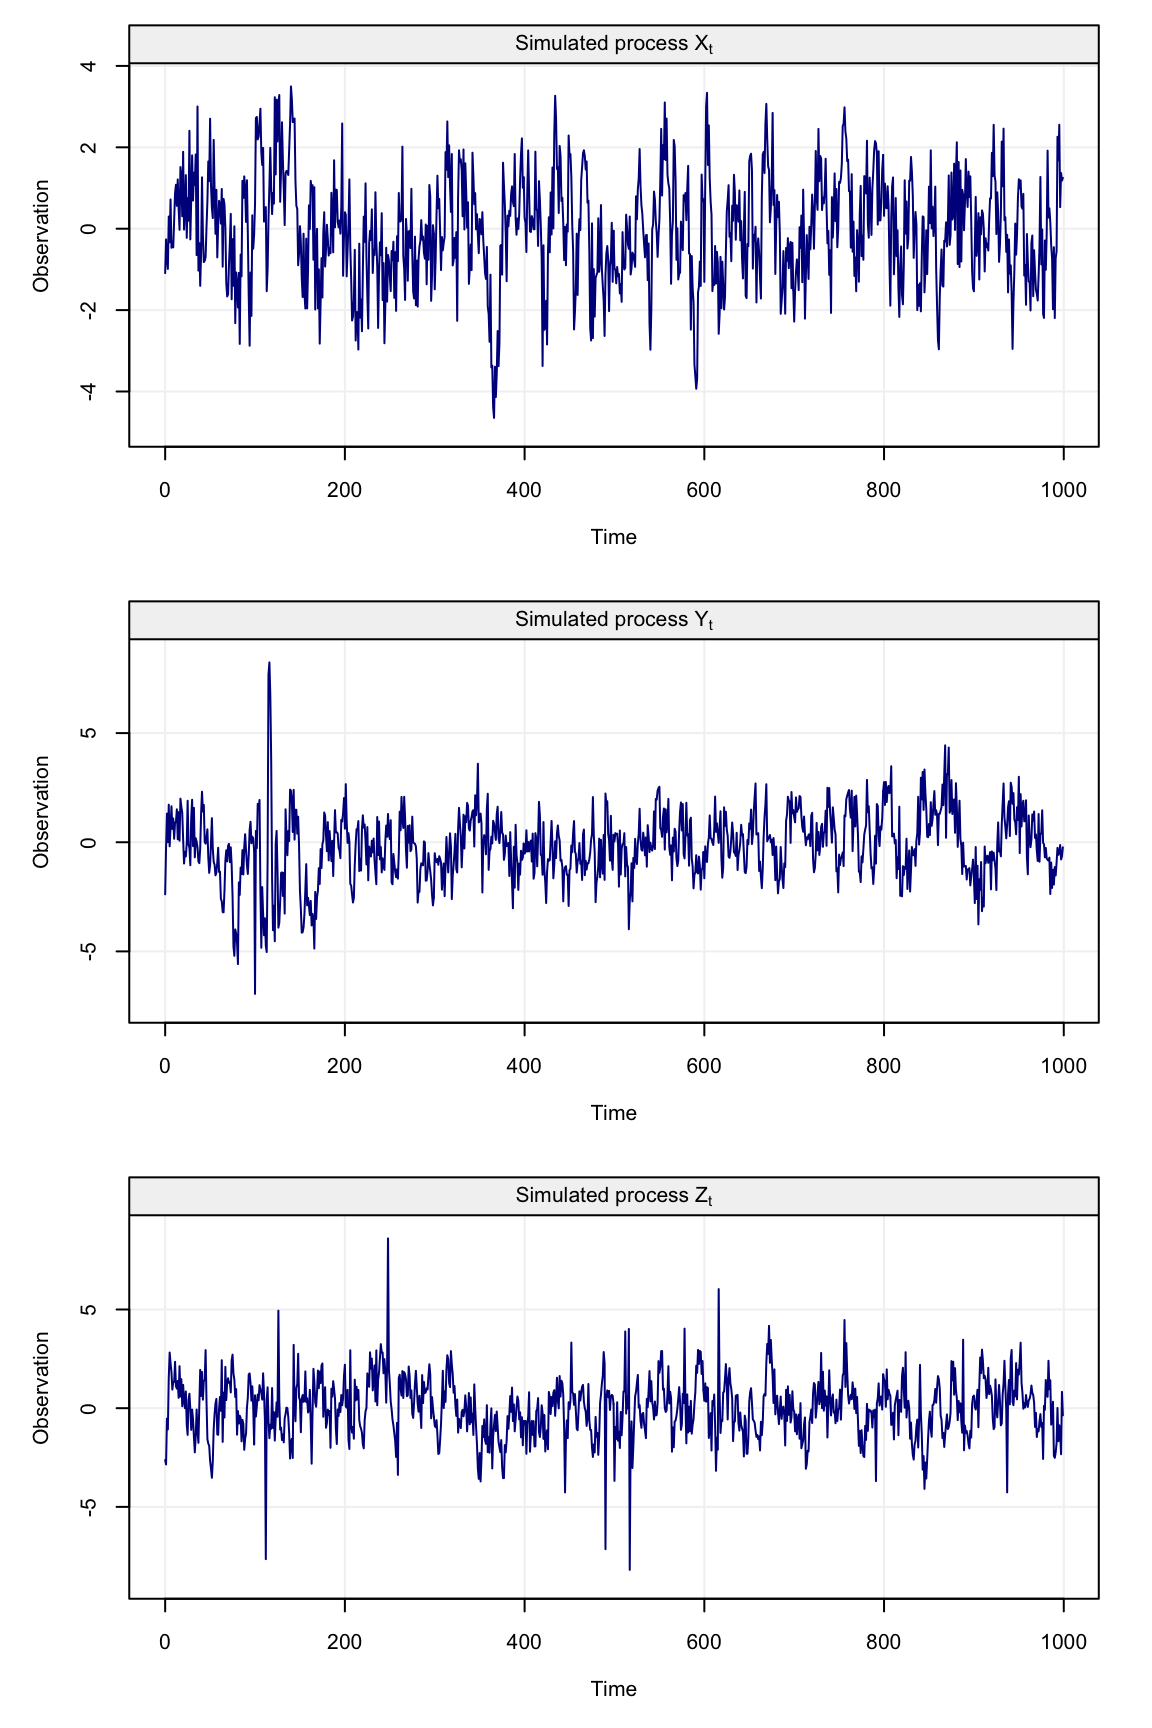
\includegraphics{tts_files/figure-latex/visualizesimuAR2data-1} 

}

\caption{Contaminated AR(2) Processes}\label{fig:visualizesimuAR2data}
\end{figure}

As every process will require the same estimation methodology, we will
first define a computational engine that will compute estimates for the
parameters across all of the different methods under the simulation
study. Doing so provides separate, reusable code that lowers the
threshold for error when compared to having multiple copies of the same
code scattered about. In addition, we have defined a means to visualize
the results obtained from the simulation study through a boxplot. The
procedure for creating the graphs is detailed after the simulation
engine.

\begin{Shaded}
\begin{Highlighting}[]
\NormalTok{sim_engine =}\StringTok{ }\ControlFlowTok{function}\NormalTok{(Xt)\{}
  \CommentTok{# Estimate ARIMA parameters using MLE}
\NormalTok{  mod =}\StringTok{ }\KeywordTok{arima}\NormalTok{(Xt, }\DataTypeTok{order =} \KeywordTok{c}\NormalTok{(}\DecValTok{2}\NormalTok{, }\DecValTok{0}\NormalTok{, }\DecValTok{0}\NormalTok{), }\DataTypeTok{include.mean  =} \OtherTok{FALSE}\NormalTok{)}
  
  \CommentTok{# Extract MLE Parameters (including sigma)}
\NormalTok{  res.MLE =}\StringTok{ }\KeywordTok{c}\NormalTok{(mod}\OperatorTok{$}\NormalTok{coef, mod}\OperatorTok{$}\NormalTok{sigma)}
  
  \CommentTok{# Calculate ACF}
\NormalTok{  autocorr =}\StringTok{ }\KeywordTok{as.numeric}\NormalTok{(}\KeywordTok{acf}\NormalTok{(Xt, }\DataTypeTok{lag.max =} \DecValTok{2}\NormalTok{, }\DataTypeTok{plot =} \OtherTok{FALSE}\NormalTok{)}\OperatorTok{$}\NormalTok{acf)}
\NormalTok{  X =}\StringTok{ }\KeywordTok{matrix}\NormalTok{(}\DecValTok{1}\NormalTok{,}\DecValTok{2}\NormalTok{,}\DecValTok{2}\NormalTok{)}
\NormalTok{  X[}\DecValTok{1}\NormalTok{,}\DecValTok{2}\NormalTok{] =}\StringTok{ }\NormalTok{X[}\DecValTok{2}\NormalTok{,}\DecValTok{1}\NormalTok{] =}\StringTok{ }\NormalTok{autocorr[}\DecValTok{2}\NormalTok{]}
\NormalTok{  y =}\StringTok{ }\NormalTok{autocorr[}\DecValTok{2}\OperatorTok{:}\DecValTok{3}\NormalTok{]}
  
  \CommentTok{# Compute Least Squares on ACF}
\NormalTok{  svmat =}\StringTok{ }\KeywordTok{solve}\NormalTok{(X)}
\NormalTok{  phi.LS =}\StringTok{ }\NormalTok{svmat}\OperatorTok\NormalTok{y}
\NormalTok{  sig2.LS =}\StringTok{ }\KeywordTok{var}\NormalTok{(Xt)}\OperatorTok{*}\NormalTok{(}\DecValTok{1} \OperatorTok{-}\StringTok{ }\KeywordTok{t}\NormalTok{(y)}\OperatorTok\NormalTok{svmat}\OperatorTok\NormalTok{y)}
\NormalTok{  res.LS =}\StringTok{ }\KeywordTok{c}\NormalTok{(phi.LS, sig2.LS)}
  
  \CommentTok{# Calculate RACF}
\NormalTok{  rob.ccf =}\StringTok{ }\KeywordTok{as.numeric}\NormalTok{(robcor}\OperatorTok{::}\KeywordTok{robacf}\NormalTok{(Xt, }\DataTypeTok{plot=}\OtherTok{FALSE}\NormalTok{, }\DataTypeTok{type =} \StringTok{"covariance"}\NormalTok{)}\OperatorTok{$}\NormalTok{acf)}
\NormalTok{  X[}\DecValTok{1}\NormalTok{,}\DecValTok{2}\NormalTok{] =}\StringTok{ }\NormalTok{X[}\DecValTok{2}\NormalTok{,}\DecValTok{1}\NormalTok{] =}\StringTok{ }\NormalTok{rob.ccf[}\DecValTok{2}\NormalTok{]}\OperatorTok{/}\NormalTok{rob.ccf[}\DecValTok{1}\NormalTok{]}
\NormalTok{  y =}\StringTok{ }\NormalTok{rob.ccf[}\DecValTok{2}\OperatorTok{:}\DecValTok{3}\NormalTok{]}\OperatorTok{/}\NormalTok{rob.ccf[}\DecValTok{1}\NormalTok{]}
  
  \CommentTok{# Compute Least Squares on RACF}
\NormalTok{  svmat =}\StringTok{ }\KeywordTok{solve}\NormalTok{(X)}
\NormalTok{  phi.RR =}\StringTok{ }\NormalTok{svmat}\OperatorTok\NormalTok{y}
\NormalTok{  sig2.RR =}\StringTok{ }\NormalTok{rob.ccf[}\DecValTok{1}\NormalTok{]}\OperatorTok{*}\NormalTok{(}\DecValTok{1} \OperatorTok{-}\StringTok{ }\KeywordTok{t}\NormalTok{(y)}\OperatorTok\NormalTok{svmat}\OperatorTok\NormalTok{y)}
\NormalTok{  res.RR =}\StringTok{ }\KeywordTok{c}\NormalTok{(phi.RR, sig2.RR)}
  
  \CommentTok{# Compute the GMWM Estimator}
\NormalTok{  res.GMWM =}\StringTok{ }\NormalTok{gmwm2}\OperatorTok{::}\KeywordTok{gmwm}\NormalTok{(}\KeywordTok{ARMA}\NormalTok{(}\DecValTok{2}\NormalTok{,}\DecValTok{0}\NormalTok{), Xt)}\OperatorTok{$}\NormalTok{estimate}
\NormalTok{  res.RGMWM =}\StringTok{ }\NormalTok{gmwm2}\OperatorTok{::}\KeywordTok{gmwm}\NormalTok{(}\KeywordTok{ARMA}\NormalTok{(}\DecValTok{2}\NormalTok{,}\DecValTok{0}\NormalTok{), Xt, }\DataTypeTok{robust =} \OtherTok{TRUE}\NormalTok{)}\OperatorTok{$}\NormalTok{estimate}

  \CommentTok{# Return results}
  \KeywordTok{list}\NormalTok{(}\DataTypeTok{res.MLE =}\NormalTok{ res.MLE, }\DataTypeTok{res.LS =}\NormalTok{ res.LS, }\DataTypeTok{res.RR =}\NormalTok{ res.RR,}
       \DataTypeTok{res.GMWM =}\NormalTok{ res.GMWM, }\DataTypeTok{res.RGMWM =}\NormalTok{ res.RGMWM)}
\NormalTok{\} }
\end{Highlighting}
\end{Shaded}

\begin{Shaded}
\begin{Highlighting}[]
\NormalTok{sim_study_graph =}\StringTok{ }\ControlFlowTok{function}\NormalTok{(res.MLE, res.LS, res.RR, res.GMWM, res.RGMWM,}
                           \DataTypeTok{Truth =} \KeywordTok{c}\NormalTok{(}\FloatTok{0.5}\NormalTok{, }\FloatTok{0.25}\NormalTok{, }\DecValTok{1}\NormalTok{))\{}
  \CommentTok{# Converts Simulation Matrices to Long Form for use in ggplot2}
\NormalTok{  d =}\StringTok{ }\NormalTok{bmisc}\OperatorTok{::}\KeywordTok{study_df}\NormalTok{(res.MLE, res.LS, res.RR, res.GMWM, res.RGMWM,}
                         \DataTypeTok{data_names =} \KeywordTok{c}\NormalTok{(}\StringTok{"MLE"}\NormalTok{,}\StringTok{"LS"}\NormalTok{,}\StringTok{"RLS"}\NormalTok{,}\StringTok{"GMWM"}\NormalTok{,}\StringTok{"RGMWM"}\NormalTok{))}
  
  \CommentTok{# Reorder factors}
\NormalTok{  d}\OperatorTok{$}\NormalTok{Draw =}\StringTok{ }\KeywordTok{factor}\NormalTok{(d}\OperatorTok{$}\NormalTok{Draw, }\DataTypeTok{levels =} \KeywordTok{c}\NormalTok{(}\DecValTok{1}\NormalTok{,}\DecValTok{2}\NormalTok{,}\DecValTok{3}\NormalTok{),}
                  \DataTypeTok{labels =} \KeywordTok{expression}\NormalTok{(phi[}\DecValTok{1}\NormalTok{], phi[}\DecValTok{2}\NormalTok{], sigma}\OperatorTok{^}\DecValTok{2}\NormalTok{))}
\NormalTok{  d}\OperatorTok{$}\NormalTok{Type =}\StringTok{ }\KeywordTok{factor}\NormalTok{(d}\OperatorTok{$}\NormalTok{Type, }\DataTypeTok{levels =} \KeywordTok{c}\NormalTok{(}\StringTok{"MLE"}\NormalTok{,}\StringTok{"LS"}\NormalTok{,}\StringTok{"RLS"}\NormalTok{,}\StringTok{"GMWM"}\NormalTok{,}\StringTok{"RGMWM"}\NormalTok{))}
  
  \CommentTok{# Add in horizontal lines}
\NormalTok{  oracle =}\StringTok{ }\KeywordTok{data.frame}\NormalTok{(}\DataTypeTok{Draw =} \DecValTok{1}\OperatorTok{:}\DecValTok{3}\NormalTok{, }\DataTypeTok{Truth =}\NormalTok{ Truth)}
\NormalTok{  oracle}\OperatorTok{$}\NormalTok{Draw =}\StringTok{ }\KeywordTok{factor}\NormalTok{(oracle}\OperatorTok{$}\NormalTok{Draw, }\DataTypeTok{levels =} \KeywordTok{c}\NormalTok{(}\DecValTok{1}\NormalTok{,}\DecValTok{2}\NormalTok{,}\DecValTok{3}\NormalTok{), }
                       \DataTypeTok{labels =} \KeywordTok{expression}\NormalTok{(phi[}\DecValTok{1}\NormalTok{], phi[}\DecValTok{2}\NormalTok{], sigma}\OperatorTok{^}\DecValTok{2}\NormalTok{))}
  
  \CommentTok{# Plot}
  \KeywordTok{ggplot}\NormalTok{(d, }\KeywordTok{aes}\NormalTok{(}\DataTypeTok{x =}\NormalTok{ Type, }\DataTypeTok{y =}\NormalTok{ Values, }\DataTypeTok{fill =}\NormalTok{ Type)) }\OperatorTok{+}\StringTok{ }
\StringTok{    }\KeywordTok{geom_boxplot}\NormalTok{() }\OperatorTok{+}\StringTok{ }
\StringTok{    }\KeywordTok{stat_boxplot}\NormalTok{(}\DataTypeTok{geom =}\StringTok{'errorbar'}\NormalTok{, }\DataTypeTok{width =} \FloatTok{0.5}\NormalTok{) }\OperatorTok{+}\StringTok{ }
\StringTok{    }\KeywordTok{geom_hline}\NormalTok{(}\DataTypeTok{data =}\NormalTok{ oracle, }\KeywordTok{aes}\NormalTok{(}\DataTypeTok{yintercept =}\NormalTok{ Truth), }\DataTypeTok{color =} \StringTok{"red"}\NormalTok{) }\OperatorTok{+}
\StringTok{    }\KeywordTok{facet_wrap}\NormalTok{(}\OperatorTok{~}\NormalTok{Draw, }\DataTypeTok{labeller =}\NormalTok{ label_parsed, }\DataTypeTok{scales =} \StringTok{"free_y"}\NormalTok{) }\OperatorTok{+}
\StringTok{    }\KeywordTok{theme_bw}\NormalTok{() }\OperatorTok{+}\StringTok{ }
\StringTok{    }\KeywordTok{theme}\NormalTok{(}\DataTypeTok{legend.position =} \StringTok{"none"}\NormalTok{,}
          \DataTypeTok{axis.text.x =} \KeywordTok{element_text}\NormalTok{(}\DataTypeTok{angle =} \DecValTok{50}\NormalTok{, }\DataTypeTok{hjust =} \DecValTok{1}\NormalTok{))}
\NormalTok{\}}
\end{Highlighting}
\end{Shaded}

With the means to now compute and visualize parameter estimates for each
of the given methods, the bootrap simulation study may now commence.
Using the simulation engine, we can simultaneously evaluate the
processes within one loop iteration. Please take into consideration that
the following simulation study is computationally intensive and may
require the amount of iteration \(B\) to be decreased on a personal
computer to complete in a reasonable time.

\begin{Shaded}
\begin{Highlighting}[]
\CommentTok{# Number of bootstrap iterations}
\NormalTok{B =}\StringTok{ }\DecValTok{250}

\CommentTok{# Simulation storage}
\NormalTok{res.xt.MLE =}\StringTok{ }\NormalTok{res.xt.LS =}\StringTok{ }\NormalTok{res.xt.RR =}\StringTok{ }\NormalTok{res.xt.GMWM =}\StringTok{ }\NormalTok{res.xt.RGMWM =}\StringTok{ }\KeywordTok{matrix}\NormalTok{(}\OtherTok{NA}\NormalTok{, B, }\DecValTok{3}\NormalTok{)}
\NormalTok{res.yt.MLE =}\StringTok{ }\NormalTok{res.yt.LS =}\StringTok{ }\NormalTok{res.yt.RR =}\StringTok{ }\NormalTok{res.yt.GMWM =}\StringTok{ }\NormalTok{res.yt.RGMWM =}\StringTok{ }\KeywordTok{matrix}\NormalTok{(}\OtherTok{NA}\NormalTok{, B, }\DecValTok{3}\NormalTok{)}
\NormalTok{res.zt.MLE =}\StringTok{ }\NormalTok{res.zt.LS =}\StringTok{ }\NormalTok{res.zt.RR =}\StringTok{ }\NormalTok{res.zt.GMWM =}\StringTok{ }\NormalTok{res.zt.RGMWM =}\StringTok{ }\KeywordTok{matrix}\NormalTok{(}\OtherTok{NA}\NormalTok{, B, }\DecValTok{3}\NormalTok{)}

\CommentTok{# Begin bootstrap}
\ControlFlowTok{for}\NormalTok{ (i }\ControlFlowTok{in} \KeywordTok{seq_len}\NormalTok{(B))\{}
  
  \CommentTok{# Set seed for reproducibility}
  \KeywordTok{set.seed}\NormalTok{(i)}
  
  \CommentTok{# Generate processes}
\NormalTok{  Xt =}\StringTok{ }\KeywordTok{gen_gts}\NormalTok{(n, }\KeywordTok{AR}\NormalTok{(}\DataTypeTok{phi =} \KeywordTok{c}\NormalTok{(}\FloatTok{0.5}\NormalTok{, }\FloatTok{0.25}\NormalTok{), }\DataTypeTok{sigma2 =} \DecValTok{1}\NormalTok{))}
\NormalTok{  Yt =}\StringTok{ }\KeywordTok{gen_gts}\NormalTok{(n, }\KeywordTok{AR}\NormalTok{(}\DataTypeTok{phi =} \KeywordTok{c}\NormalTok{(}\FloatTok{0.5}\NormalTok{, }\FloatTok{0.25}\NormalTok{), }\DataTypeTok{sigma2 =} \DecValTok{1}\NormalTok{))}
\NormalTok{  Zt =}\StringTok{ }\KeywordTok{gen_gts}\NormalTok{(n, }\KeywordTok{AR}\NormalTok{(}\DataTypeTok{phi =} \KeywordTok{c}\NormalTok{(}\FloatTok{0.5}\NormalTok{, }\FloatTok{0.25}\NormalTok{), }\DataTypeTok{sigma2 =} \DecValTok{1}\NormalTok{))}
  
  \CommentTok{# Generate Ut contamination process that replaces a portion of original signal}
\NormalTok{  Yt[}\DecValTok{101}\OperatorTok{:}\DecValTok{135}\NormalTok{] =}\StringTok{ }\KeywordTok{gen_gts}\NormalTok{(}\DecValTok{35}\NormalTok{, }\KeywordTok{AR}\NormalTok{(}\DataTypeTok{phi =} \KeywordTok{c}\NormalTok{(}\FloatTok{0.9}\NormalTok{,}\OperatorTok{-}\FloatTok{0.4}\NormalTok{), }\DataTypeTok{sigma2 =} \DecValTok{9}\NormalTok{))}
  
  \CommentTok{# Generate Nt contamination that inject noise at random}
\NormalTok{  Zt[}\KeywordTok{sample}\NormalTok{(n, dispersal, }\DataTypeTok{replace =} \OtherTok{FALSE}\NormalTok{)] =}\StringTok{ }\KeywordTok{gen_gts}\NormalTok{(dispersal, }\KeywordTok{WN}\NormalTok{(}\DataTypeTok{sigma2 =} \DecValTok{9}\NormalTok{))}

  \CommentTok{# Compute estimates and store in the appropriate matrix}
\NormalTok{  res =}\StringTok{ }\KeywordTok{sim_engine}\NormalTok{(Xt)}
\NormalTok{  res.xt.MLE[i,]  =}\StringTok{ }\NormalTok{res}\OperatorTok{$}\NormalTok{res.MLE; res.xt.LS[i,] =}\StringTok{ }\NormalTok{res}\OperatorTok{$}\NormalTok{res.LS; res.xt.RR[i,] =}\StringTok{ }\NormalTok{res}\OperatorTok{$}\NormalTok{res.RR}
\NormalTok{  res.xt.GMWM[i,] =}\StringTok{ }\NormalTok{res}\OperatorTok{$}\NormalTok{res.GMWM;res.xt.RGMWM[i,] =}\StringTok{ }\NormalTok{res}\OperatorTok{$}\NormalTok{res.RGMWM}
  
\NormalTok{  res =}\StringTok{ }\KeywordTok{sim_engine}\NormalTok{(Yt)}
\NormalTok{  res.yt.MLE[i,]  =}\StringTok{ }\NormalTok{res}\OperatorTok{$}\NormalTok{res.MLE; res.yt.LS[i,] =}\StringTok{ }\NormalTok{res}\OperatorTok{$}\NormalTok{res.LS; res.yt.RR[i,] =}\StringTok{ }\NormalTok{res}\OperatorTok{$}\NormalTok{res.RR}
\NormalTok{  res.yt.GMWM[i,] =}\StringTok{ }\NormalTok{res}\OperatorTok{$}\NormalTok{res.GMWM;res.yt.RGMWM[i,] =}\StringTok{ }\NormalTok{res}\OperatorTok{$}\NormalTok{res.RGMWM}

\NormalTok{  res =}\StringTok{ }\KeywordTok{sim_engine}\NormalTok{(Zt)}
\NormalTok{  res.zt.MLE[i,]  =}\StringTok{ }\NormalTok{res}\OperatorTok{$}\NormalTok{res.MLE; res.zt.LS[i,] =}\StringTok{ }\NormalTok{res}\OperatorTok{$}\NormalTok{res.LS; res.zt.RR[i,] =}\StringTok{ }\NormalTok{res}\OperatorTok{$}\NormalTok{res.RR}
\NormalTok{  res.zt.GMWM[i,] =}\StringTok{ }\NormalTok{res}\OperatorTok{$}\NormalTok{res.GMWM;res.zt.RGMWM[i,] =}\StringTok{ }\NormalTok{res}\OperatorTok{$}\NormalTok{res.RGMWM}
\NormalTok{\}}
\end{Highlighting}
\end{Shaded}

\begin{figure}
\centering
\includegraphics{tts_files/figure-latex/simuAR2XtResults-1.pdf}
\caption{\label{fig:simuAR2XtResults}Estimation of Uncontaminated AR(2)
Process}
\end{figure}

\begin{figure}
\centering
\includegraphics{tts_files/figure-latex/simuAR2YtResults-1.pdf}
\caption{\label{fig:simuAR2YtResults}Estimation of Contaminated AR(2)
Process with a Secondary Process}
\end{figure}

\begin{figure}
\centering
\includegraphics{tts_files/figure-latex/simAR2ZtResults-1.pdf}
\caption{\label{fig:simAR2ZtResults}Estimation of Contaminated AR(2) Process
with Random Noise Injected}
\end{figure}

After performing the estimation, we opt to visually assess how well each
methodology performed. We begin by observing the baseline case regarding
the the uncontaminated sample \(X_t\) given in Figure
\ref{fig:simuAR2XtResults}. Within this context, the estimation methods
appear to performing equally across all parameters. Note, it may appear
as if \(\phi_2\) had a noticable departure from the truth, however, the
difference presented is minor considering the y-axis of the graph and
parameter recovery present elsewhere. Turning our attention to Figure
\ref{fig:simuAR2YtResults}, which displays results from estimating
\(Y_t\), the process with partial contamination from another; the robust
methodologies (R-LS, RGMWM) were able to effectively handle the
contamination when compared to the classical approaches (LS, MLE, GMWM)
missed the mark greatly on several estimates. From the simulations,
there is evidence to suggest that additional study should be performed
to assess the performance of R-LS vs.~RGMWM. Lastly, we consider the
results of estimating \(Z_t\), the case of random noise injected into
the process, given in Figure \ref{fig:simAR2ZtResults}. The noise has a
troubling impact with respect to estimating the large \(\phi_1\) and
\(\sigma^2\). However, the estimation procedure appear to be able to
reasonably capture \(\phi_2\). As shown previously, the robust
techniques provide better estimations than their counterparts.

For all the above methods, it would be necessary to understand how
``precise'' their estimates are. To do so we would need to obtain
confidence intervals for these estimates and this can be done mainly in
two manners:

\begin{itemize}
\tightlist
\item
  using the asymptotic distribution of the parameter estimates;
\item
  using parametric bootstrap.
\end{itemize}

The first approach consists in using the asymptotic distribution of the
estimators presented earlier to deliver approximations of the confidence
intervals which get better as the length of the observed time series
increases. Hence, for example, if we wanted to find a 95\% confidence
interval for the parameter \(\phi\), we would use the quantiles of the
normal distribution (given that all methods presented earlier present
this asymptotic distribution). However, this approach can present some
drawbacks, one of which is there behaviour when the parameters are close
to the boundaries of the parameter space. Suppose we consider a
realization of length \(n = 100\) of the following AR(1) model:

\[X_t = 0.96 X_{t-1} + W_t, \;\;\;\; W_t \sim \mathcal{N}(0,1),\]

which is depicted in Figure \ref{fig:simAR1ci}

\begin{Shaded}
\begin{Highlighting}[]
\KeywordTok{set.seed}\NormalTok{(}\DecValTok{7}\NormalTok{)}
\NormalTok{x =}\StringTok{ }\KeywordTok{gen_gts}\NormalTok{(}\DataTypeTok{n =} \DecValTok{100}\NormalTok{, }\KeywordTok{AR1}\NormalTok{(}\FloatTok{0.96}\NormalTok{, }\DecValTok{1}\NormalTok{))}
\KeywordTok{plot}\NormalTok{(x)}
\end{Highlighting}
\end{Shaded}

\begin{figure}
\centering
\includegraphics{tts_files/figure-latex/simAR1ci-1.pdf}
\caption{\label{fig:simAR1ci}AR(1) with \(\phi\) close to parameter bound}
\end{figure}

It can be seen that the parameter \(\phi = 0.96\) respects the condition
for stationarity, \(\left| \phi \right| < 1\), but is very close to its
boundary. Using the MLE and the GMWM estimators, we first estimate the
parameters and then compute confidence intervals for \(\phi\) using the
asymptotic normal distribution.

\begin{Shaded}
\begin{Highlighting}[]
\CommentTok{# Compute the parameter estimates using MLE}
\NormalTok{fit.ML =}\StringTok{ }\KeywordTok{arima}\NormalTok{(x, }\DataTypeTok{order =} \KeywordTok{c}\NormalTok{(}\DecValTok{1}\NormalTok{,}\DecValTok{0}\NormalTok{,}\DecValTok{0}\NormalTok{), }\DataTypeTok{include.mean =} \OtherTok{FALSE}\NormalTok{)}
\KeywordTok{c}\NormalTok{(}\StringTok{"phi"}\NormalTok{ =}\StringTok{ }\NormalTok{fit.ML}\OperatorTok{$}\NormalTok{coef, }\StringTok{"se"}\NormalTok{ =}\StringTok{ }\KeywordTok{sqrt}\NormalTok{(fit.ML}\OperatorTok{$}\NormalTok{var.coef))}
\end{Highlighting}
\end{Shaded}

\begin{verbatim}
##    phi.ar1         se 
## 0.96718451 0.02026333
\end{verbatim}

\begin{Shaded}
\begin{Highlighting}[]
\CommentTok{# Construct asymptotic confidence interval for phi}
\NormalTok{fit.ML}\OperatorTok{$}\NormalTok{coef }\OperatorTok{+}\StringTok{ }\KeywordTok{c}\NormalTok{(}\OperatorTok{-}\DecValTok{1}\NormalTok{,}\DecValTok{1}\NormalTok{)}\OperatorTok{*}\FloatTok{1.96}\OperatorTok{*}\KeywordTok{as.numeric}\NormalTok{(}\KeywordTok{sqrt}\NormalTok{(fit.ML}\OperatorTok{$}\NormalTok{var.coef))}
\end{Highlighting}
\end{Shaded}

\begin{verbatim}
## [1] 0.9274684 1.0069006
\end{verbatim}

\begin{Shaded}
\begin{Highlighting}[]
\CommentTok{# Compute the parameter estimates with inference using GMWM}
\NormalTok{fit.gmwm =}\StringTok{ }\NormalTok{gmwm2}\OperatorTok{::}\KeywordTok{gmwm}\NormalTok{(}\KeywordTok{AR1}\NormalTok{(), x)}
\KeywordTok{summary}\NormalTok{(fit.gmwm, }\DataTypeTok{inference =} \OtherTok{TRUE}\NormalTok{)}\OperatorTok{$}\NormalTok{estimate}
\end{Highlighting}
\end{Shaded}

\begin{verbatim}
##        Estimates    CI Low  CI High         SE
## AR1    0.9828707 0.8273193 1.063385 0.07175885
## SIGMA2 0.9640085 0.6910088 1.156587 0.14152576
\end{verbatim}

From the estimation summary, we note that both confidence intervals
contain values that would make the AR(1) non-stationary (i.e.~values of
\(\phi\) larger than 1). These estimates are indicating that they
represent the estimated (asymptotic) distribution of \(\hat{\phi}\) as
displayed in Figure \ref{fig:asymIC}.

\begin{figure}
\centering
\includegraphics{tts_files/figure-latex/asymIC-1.pdf}
\caption{\label{fig:asymIC}Estimated asymptotic distribution of
\(\hat{\phi}\) for MLE and GMWM parameter estimates. The dashed vertical
line represents the true value of \(\phi\), the solid line denotes the
upper bound of the parameter space for \(\phi\) and the vertical ticks
represent the limits of the 95\% confidence intervals for both methods.}
\end{figure}

For this purpose, the confidence intervals are not realistic. Therefore,
one viable solution is to employ a parametric bootstrap, detailed in
Theorem \ref{thm:parabootstrap}. Indeed, parametric bootstrap takes the
estimated parameter values and uses them in order to simulate from an
AR(1) process. For each simulation, the parameters are estimated again
and stored. Finally, the empirical quantiles at \(\alpha/2\) and
\(1-\alpha/2\) are taken of the saved estimated parameter values to
obtrain a confidence interval which does not suffer from boundary
problems. The code below gives an example of how this confidence
interval is built based on the same estimation procedure but using
parametric bootstrap (using \(B = 10000\) bootstrap replicates).

\begin{Shaded}
\begin{Highlighting}[]
\CommentTok{# Number of Iterations}
\NormalTok{B =}\StringTok{ }\DecValTok{10000}

\CommentTok{# Set up storage for results}
\NormalTok{est.phi.gmwm =}\StringTok{ }\KeywordTok{rep}\NormalTok{(}\OtherTok{NA}\NormalTok{,B)}
\NormalTok{est.phi.ML =}\StringTok{ }\KeywordTok{rep}\NormalTok{(}\OtherTok{NA}\NormalTok{,B)}

\CommentTok{# Model generation statements}
\NormalTok{model.gmwm =}\StringTok{ }\KeywordTok{AR1}\NormalTok{(fit.gmwm}\OperatorTok{$}\NormalTok{estimate[}\DecValTok{1}\NormalTok{], fit.gmwm}\OperatorTok{$}\NormalTok{estimate[}\DecValTok{2}\NormalTok{])}
\NormalTok{model.mle =}\StringTok{ }\KeywordTok{AR1}\NormalTok{(fit.ML}\OperatorTok{$}\NormalTok{coef, fit.ML}\OperatorTok{$}\NormalTok{sigma2)}

\CommentTok{# Begin bootstrap}
\ControlFlowTok{for}\NormalTok{(i }\ControlFlowTok{in} \KeywordTok{seq_len}\NormalTok{(B))\{}
  
  \CommentTok{# Set seed for reproducibility}
  \KeywordTok{set.seed}\NormalTok{(B }\OperatorTok{+}\StringTok{ }\NormalTok{i)}
  
  \CommentTok{# Generate process under MLE parameter estimate}
\NormalTok{  x.star =}\StringTok{ }\KeywordTok{gen_gts}\NormalTok{(}\DecValTok{100}\NormalTok{, model.mle)}
  
  \CommentTok{# Attempt to estimate phi by employing a try}
\NormalTok{  est.phi.ML[i] =}\StringTok{ }\KeywordTok{tryCatch}\NormalTok{(}\KeywordTok{arima}\NormalTok{(x.star, }\DataTypeTok{order =} \KeywordTok{c}\NormalTok{(}\DecValTok{1}\NormalTok{,}\DecValTok{0}\NormalTok{,}\DecValTok{0}\NormalTok{), }\DataTypeTok{include.mean =} \OtherTok{FALSE}\NormalTok{)}\OperatorTok{$}\NormalTok{coef, }
                           \DataTypeTok{error =} \ControlFlowTok{function}\NormalTok{(e) }\OtherTok{NA}\NormalTok{)}
  
  \CommentTok{# Generate process under GMWM parameter estimate}
\NormalTok{  x.star =}\StringTok{ }\KeywordTok{gen_gts}\NormalTok{(}\DecValTok{100}\NormalTok{, model.gmwm)}
\NormalTok{  est.phi.gmwm[i] =}\StringTok{ }\NormalTok{gmwm2}\OperatorTok{::}\KeywordTok{gmwm}\NormalTok{(model.gmwm, x.star)}\OperatorTok{$}\NormalTok{estimate[}\DecValTok{1}\NormalTok{]}
\NormalTok{\}}
\end{Highlighting}
\end{Shaded}

\begin{figure}
\centering
\includegraphics{tts_files/figure-latex/paraAR1cigraphs-1.pdf}
\caption{\label{fig:paraAR1cigraphs}Estimated parametric distributions of
\(\hat{\phi}\) for MLE and GMWM parameter estimates. The bar plots
represent the results from the parametric bootstrap, the densities
represent the estimate asymptotic distribution, the vertical line
represents the true value of \(\phi\), the solid lines denotes the upper
bound of the parameter space for \(\phi\) and the vertical ticks
represent the limits of the 95\% confidence intervals under both
approaches for the estimation methods.}
\end{figure}

In Figure \ref{fig:paraAR1cigraphs}, we compare the estimated densities
for \(\hat{\phi}\) using asymptotic results and bootstrap techniques for
the MLE and the GMWM estimator. It can be observed that the issue that
arose previously with unrealistic confidence intervals have been
resolved as the interval regions lie entirely within the boundaries of
the parameter space.

To emphasize that the effectiveness of parametric bootstrap, let us
consider one additonal example of an AR(2) process. For this example,
discussion will focus on observing the behavior exhibited solely by the
MLE. Having said this, the AR(2) process is defined to be:

\begin{equation}
{X_t} = {1.98}{X_{t - 1}} - {0.99}{X_{t - 2}} + {W_t}
\label{eq:ciar2}
\end{equation}

where \(W_t \sim WN(0, 1)\). The generated process is displayed in
Figure \ref{fig:CIAR2data}.

\begin{Shaded}
\begin{Highlighting}[]
\KeywordTok{set.seed}\NormalTok{(}\DecValTok{432}\NormalTok{)}
\NormalTok{Xt =}\StringTok{ }\KeywordTok{gen_gts}\NormalTok{(}\DecValTok{500}\NormalTok{, }\KeywordTok{AR}\NormalTok{(}\DataTypeTok{phi =} \KeywordTok{c}\NormalTok{(}\FloatTok{1.98}\NormalTok{, }\FloatTok{-0.99}\NormalTok{), }\DataTypeTok{sigma2 =} \DecValTok{1}\NormalTok{))}
\KeywordTok{plot}\NormalTok{(Xt)}
\end{Highlighting}
\end{Shaded}

\begin{figure}
\centering
\includegraphics{tts_files/figure-latex/CIAR2data-1.pdf}
\caption{\label{fig:CIAR2data}Generated AR(2) Process}
\end{figure}

\begin{Shaded}
\begin{Highlighting}[]
\NormalTok{mod =}\StringTok{ }\KeywordTok{arima}\NormalTok{(Xt, }\KeywordTok{c}\NormalTok{(}\DecValTok{2}\NormalTok{,}\DecValTok{0}\NormalTok{,}\DecValTok{0}\NormalTok{), }\DataTypeTok{include.mean =} \OtherTok{FALSE}\NormalTok{)}
\NormalTok{mod}
\end{Highlighting}
\end{Shaded}

\begin{verbatim}
## 
## Call:
## arima(x = Xt, order = c(2, 0, 0), include.mean = FALSE)
## 
## Coefficients:
##          ar1      ar2
##       1.9787  -0.9892
## s.e.  0.0053   0.0052
## 
## sigma^2 estimated as 0.8419:  log likelihood = -672.58,  aic = 1351.15
\end{verbatim}

With the model's coefficients readily available, the parametric
bootstrap is able to be constructed. As before, the bootstrap
implementation mirrors prior versions with one cavaet regarding the
storage of \(\phi\) being two dimensional and, thus, requiring a
\texttt{matrix} to store the result instead of a traditional atomic
vector in \emph{R}.

\begin{Shaded}
\begin{Highlighting}[]
\NormalTok{B =}\StringTok{ }\DecValTok{10000}
\NormalTok{est.phi.ML =}\StringTok{ }\KeywordTok{matrix}\NormalTok{(}\OtherTok{NA}\NormalTok{, B, }\DecValTok{2}\NormalTok{)}
\NormalTok{model =}\StringTok{ }\KeywordTok{AR}\NormalTok{(}\DataTypeTok{phi =}\NormalTok{ mod}\OperatorTok{$}\NormalTok{coef, }\DataTypeTok{sigma2 =}\NormalTok{ mod}\OperatorTok{$}\NormalTok{sigma2)}

\ControlFlowTok{for}\NormalTok{(i }\ControlFlowTok{in} \KeywordTok{seq_len}\NormalTok{(B)) \{}
  \KeywordTok{set.seed}\NormalTok{(B }\OperatorTok{+}\StringTok{ }\NormalTok{i)              }\CommentTok{# Set Seed for reproducibilty}
  
\NormalTok{  x.star =}\StringTok{ }\KeywordTok{gen_gts}\NormalTok{(}\DecValTok{500}\NormalTok{, model) }\CommentTok{# Simulate the process }
  
  \CommentTok{# Obtain parameter estimate with protection}
  \CommentTok{# that defaults to NA if unable to estimate}
\NormalTok{  est.phi.ML[i,] =}\StringTok{ }\KeywordTok{tryCatch}\NormalTok{(}\KeywordTok{arima}\NormalTok{(x.star, }\DataTypeTok{order =} \KeywordTok{c}\NormalTok{(}\DecValTok{2}\NormalTok{,}\DecValTok{0}\NormalTok{,}\DecValTok{0}\NormalTok{),}
                                  \DataTypeTok{include.mean =} \OtherTok{FALSE}\NormalTok{)}\OperatorTok{$}\NormalTok{coef,}
                            \DataTypeTok{error =} \ControlFlowTok{function}\NormalTok{(e) }\OtherTok{NA}\NormalTok{)}
\NormalTok{\}}
\end{Highlighting}
\end{Shaded}

\begin{figure}
\centering
\includegraphics{tts_files/figure-latex/ciAR2d-1.pdf}
\caption{\label{fig:ciAR2d}Estimated distributions of \(\hat{\phi_1}\) and
\(\hat{\phi_2}\) of the MLE using asymptotic and parametric bootstrap
techniques. The colored contours represent the density of distribution
and the dark grey lines represent the boundary constraints of
\(\left|\phi_2\right|<1\) and \(\phi_2 = 1 - \phi_1\).}
\end{figure}

The cost of this approach is the assumption the model captures the
dependency structure that is present within the time series. That is to
say, we are able to successfully a regenerate new time series process
that follows the appropriate distribution for each sampling phase.
However, if we are not confident that the model we have selected is a
valid estimation of the truth, then using parametric bootstrap with the
estimated model is highly problematic as it does not represent the
dependency between observations. To complicate matters further, the
traditional bootstrap that consists of simple random sampling with
replacement, in the presence of dependency, would also be highly
inaccurate and downright reckless to use. Therefore, to preserve the
dependency structure of the original data one would have to use
\emph{block bootstrapping}, which is a form of non-parametric bootstrap.
There are many different kinds of block bootstraps for time series,
which are descendents of the Moving Block Bootstrap (MBB) presented in
\ref{thm:mbb}.

\BeginKnitrBlock{theorem}
\protect\hypertarget{thm:mbb}{}{\label{thm:mbb} }Suppose that
\(\left(X_t\right)\) is weakly stationary time series with \(N\)
observations.

\begin{enumerate}
\def\labelenumi{\arabic{enumi}.}
\tightlist
\item
  Divide time series into overlapping blocks
  \(\left\{S_1, \ldots, S_M\right\}\) of length \(\ell\),
  \(1 \le \ell < N\), resulting in \(M = N - \ell + 1\) blocks
  structured as:
\end{enumerate}

\[\begin{aligned}   
  {S_1}& = & ({X_1}, &{X_2}, \cdots , {X_\ell}) & && \\
  {S_2}& = & &( {X_2}, {X_3}, \cdots , {X_{\ell + 1}}) & && \\
  & \cdots & & {} & \cdots && \\
  {S_M} & = & & & {} &&( {X_{N-\ell+1}}, {X_{N-\ell+2}}, \cdots , {X_{N}})
\end{aligned}\]

\begin{enumerate}
\def\labelenumi{\arabic{enumi}.}
\setcounter{enumi}{1}
\tightlist
\item
  Draw \(M = \left\lfloor {\frac{N}{\ell}} \right\rfloor\) blocks with
  replacement from these \(\left\{S_1, \ldots, S_M\right\}\) blocks and
  place them in order to form \((X_t^*)\).
\item
  Compute the statistic of interest on the simulated sample \((X_t^*)\).
\item
  Repeat Steps 2 and 3 \(B\) times where \(B\) is sufficiently ``large''
  (typically \(100 \leq B \leq 10000\)).
\item
  Compute the empirical mean and variance on the statistic of interest
  based on the \(B\) independent replications.

  \EndKnitrBlock{theorem}
\end{enumerate}

The approach taken by MBB ensures that within each block the dependency
between observations is preserved. Though, one particular issue that now
arises is that some inaccuracy is introduced as a result of successive
blocks potentially being independent from each other. In reality, this
is one of the trade-offs of the MBB approach that can be mitigated by
selecting an optimal \(\ell\). To lower the inaccuracy of the procedure
the selection of \(\ell = N^{1/3}\) as \(N \to \infty\) is optimal
(proof left as an exercise to the reader). An earlier variant of MBB was
called nonoverlapping block bootstrap (NBB), which prohbited the sharing
of data described in \ref{thm:nbb}.

\BeginKnitrBlock{theorem}
\protect\hypertarget{thm:nbb}{}{\label{thm:nbb} }Suppose that
\(\left(X_t\right)\) is weakly stationary time series with \(N\)
observations.

\begin{enumerate}
\def\labelenumi{\arabic{enumi}.}
\tightlist
\item
  Divide time series into nonoverlapping blocks
  \(\left\{S_1, \ldots, S_M\right\}\) of length \(\ell\),
  \(1 \le \ell < N\), resulting in
  \(M = \left\lfloor {\frac{N}{\ell}} \right\rfloor\) blocks structured
  as:
\end{enumerate}

\[\begin{aligned}   
  {S_1}& = & ({X_1}, {X_2}, \cdots , {X_\ell})& & && \\
  {S_2}& = & &( {X_{\ell+1}}, {X_{\ell+2}}, \cdots , {X_{2\ell}}) & && \\
  & \cdots & & {} & \cdots && \\
  {S_K} & = & & & {} &&( {X_{\left({}\right)}}, {X_{N-\ell+2}}, \cdots , {X_{N}})
\end{aligned}\]

\begin{enumerate}
\def\labelenumi{\arabic{enumi}.}
\setcounter{enumi}{1}
\tightlist
\item
  Draw \(M\) blocks with replacement from these
  \(\left\{S_1, \ldots, S_M\right\}\) blocks and place them in order to
  form \((X_t^*)\).
\item
  Compute the statistic of interest on the simulated sample \((X_t^*)\).
\item
  Repeat Steps 2 and 3 \(B\) times where \(B\) is sufficiently ``large''
  (typically \(100 \leq B \leq 10000\)).
\item
  Compute the empirical mean and variance on the statistic of interest
  based on the \(B\) independent replications.
\end{enumerate}
\EndKnitrBlock{theorem}

Alternatively, depending on the case one can also use modification of
MBB that seeks to change how the beginning and end of the time series is
weighted such as a circular block-bootstrap (CBB), that seeks improve
dependency by wrapping observations, or a stationary bootstrap (SB),
that randomizes block length by under a geometric distribution of mean
\(\ell\). Regardless, the outcomes from using MBB on time series is
considerably better than just resampling, which is also possible if we
set \(\ell = 1\) since the length of \((X_t^*)\) is \(M\times\ell\).

Having said this, the implementation of Theorem \ref{thm:nbb} follows
the similar mold of generating data, estimating, and returning a value.
The most notably deviation from Theorem \ref{thm:nbb} is the use of an
indexing trick to indicate the start period of each block that allows
for only one copy of the data to be held within memory instead of \(m\)
blocks of length \(\ell\) in addition to the initial copy.

\begin{Shaded}
\begin{Highlighting}[]
\NormalTok{ar1_blockboot =}\StringTok{ }\ControlFlowTok{function}\NormalTok{(Xt, }\DataTypeTok{block_len =} \DecValTok{10}\NormalTok{, }\DataTypeTok{B =} \DecValTok{500}\NormalTok{) \{}
  
\NormalTok{  n =}\StringTok{ }\KeywordTok{length}\NormalTok{(Xt)            }\CommentTok{# Length of Time Series}
\NormalTok{  res =}\StringTok{ }\KeywordTok{rep}\NormalTok{(}\OtherTok{NA}\NormalTok{, B)          }\CommentTok{# Bootstrapped Statistics}
\NormalTok{  m =}\StringTok{ }\KeywordTok{floor}\NormalTok{(n}\OperatorTok{/}\NormalTok{block_len)    }\CommentTok{# Amount of Blocks}
  
  \ControlFlowTok{for}\NormalTok{ (i }\ControlFlowTok{in} \KeywordTok{seq_len}\NormalTok{(B)) \{   }\CommentTok{# Begin MMB}
    
    \KeywordTok{set.seed}\NormalTok{(i }\OperatorTok{+}\StringTok{ }\DecValTok{1199}\NormalTok{)      }\CommentTok{# Set seed for reproducibility}
\NormalTok{    x_star =}\StringTok{ }\KeywordTok{rep}\NormalTok{(}\OtherTok{NA}\NormalTok{, n)     }\CommentTok{# Setup storage for new TS}
    
    \ControlFlowTok{for}\NormalTok{ (j }\ControlFlowTok{in} \KeywordTok{seq_len}\NormalTok{(m)) \{ }\CommentTok{# Simulate new time series }
      
\NormalTok{      index =}\StringTok{ }\KeywordTok{sample}\NormalTok{(m, }\DecValTok{1}\NormalTok{)  }\CommentTok{# Randomize block starting points}
      
      \CommentTok{# Place block into time series}
\NormalTok{      x_star[(block_len}\OperatorTok{*}\NormalTok{(j }\OperatorTok{-}\StringTok{ }\DecValTok{1}\NormalTok{) }\OperatorTok{+}\StringTok{ }\DecValTok{1}\NormalTok{)}\OperatorTok{:}\NormalTok{(block_len}\OperatorTok{*}\NormalTok{j)] =}\StringTok{ }
\StringTok{            }\NormalTok{Xt[(block_len}\OperatorTok{*}\NormalTok{(index }\OperatorTok{-}\StringTok{ }\DecValTok{1}\NormalTok{) }\OperatorTok{+}\StringTok{ }\DecValTok{1}\NormalTok{)}\OperatorTok{:}\NormalTok{(block_len}\OperatorTok{*}\NormalTok{index)]}
\NormalTok{    \}}
    
    \CommentTok{# Calculate parameter with protection}
\NormalTok{    res[i] =}\StringTok{ }\KeywordTok{tryCatch}\NormalTok{(}\KeywordTok{arima}\NormalTok{(x_star, }\DataTypeTok{order =} \KeywordTok{c}\NormalTok{(}\DecValTok{1}\NormalTok{,}\DecValTok{0}\NormalTok{,}\DecValTok{0}\NormalTok{), }\DataTypeTok{include.mean =} \OtherTok{FALSE}\NormalTok{)}\OperatorTok{$}\NormalTok{coef,}
                      \DataTypeTok{error =} \ControlFlowTok{function}\NormalTok{(e) }\OtherTok{NA}\NormalTok{)}
\NormalTok{  \}}
  
  \KeywordTok{na.omit}\NormalTok{(res)              }\CommentTok{# Release bootstrap result}
\NormalTok{\}}
\end{Highlighting}
\end{Shaded}

With the block bootstrapping technique in hand, let us consider a
scenario where the model's assumption that the residuals will be
Gaussian is violated. Consider two AR(1) processes with the same
coefficient but different noise generation procedures:

\[
\begin{aligned}
\mathcal{M}_1:&{}& X_t &=0.5 X_{t-1} + W_t,&{}& W_t\sim \mathcal{N} (0,1) \\
\mathcal{M}_2:&{}& X_t &=0.5 X_{t-1} + V_t,&{}& V_t\sim t_4
\end{aligned}
\] The generation procedure for \(\mathcal{M}_1\) is straightforward,
use: \texttt{gen\_gts()}. However, the underlying generating mechanism
for \texttt{gen\_gts()} relies upon the noise being Gaussian. Therefore,
to generate \(\mathcal{M}_2\), one must use \emph{R}'s
\texttt{arima.sim()} function with a custom noise generator defined to
sample from a \(t\) distribution.

\begin{Shaded}
\begin{Highlighting}[]
\KeywordTok{set.seed}\NormalTok{(}\DecValTok{1}\NormalTok{)                                        }\CommentTok{# Set seed for reproducibilty}
\NormalTok{xt_m1 =}\StringTok{ }\KeywordTok{gen_gts}\NormalTok{(}\DecValTok{500}\NormalTok{, }\KeywordTok{AR1}\NormalTok{(}\DataTypeTok{phi =} \FloatTok{0.5}\NormalTok{, }\DataTypeTok{sigma2 =} \DecValTok{1}\NormalTok{))   }\CommentTok{# Gaussian noise only}
\NormalTok{xt_m2 =}\StringTok{ }\KeywordTok{arima.sim}\NormalTok{(}\DataTypeTok{n =} \DecValTok{500}\NormalTok{, }\KeywordTok{list}\NormalTok{(}\DataTypeTok{ar =} \FloatTok{0.5}\NormalTok{, }\DataTypeTok{ma =} \DecValTok{0}\NormalTok{), }\CommentTok{# Multiple noises supported}
                  \DataTypeTok{rand.gen =} \ControlFlowTok{function}\NormalTok{(n, ...) }\KeywordTok{rt}\NormalTok{(n, }\DataTypeTok{df =} \DecValTok{4}\NormalTok{))}
\end{Highlighting}
\end{Shaded}

\begin{figure}
\centering
\includegraphics{tts_files/figure-latex/mbbdatavis-1.pdf}
\caption{\label{fig:mbbdatavis}AR(1) processes generated under different
noise conditions.}
\end{figure}

From Figure \ref{fig:mbbdatavis}, the time series look remarkably
different as a result of the noise process being altered slightly even
though the \(\phi\) coefficient was held constant. Principally, the
difference is the due related to the variance of the \(t\) distribution
is defined to be \(\frac{\nu}{\nu-2}\) for \(\nu > 2\) and \(\infty\)
for \(\nu \le 2\). Therefore, the i.i.d white noise processes generated
are \(\sigma^2_{\mathcal{M}_1} = 1\) when compared to the alternative
\(\sigma^2_{\mathcal{M}_2} = 2\). With this being said, both the
underlying nonparametric and parametric bootstrap estimation procedures
betweenthe models will be the same. The implementation for blocking
approach regarding an AR(1) was discussed previously and the parametric
approach is as follows:

\begin{Shaded}
\begin{Highlighting}[]
\NormalTok{ar1_paraboot =}\StringTok{ }\ControlFlowTok{function}\NormalTok{(model, }\DataTypeTok{B =} \DecValTok{10000}\NormalTok{) \{}
\NormalTok{  est.phi =}\StringTok{ }\KeywordTok{rep}\NormalTok{(}\OtherTok{NA}\NormalTok{,B)    }\CommentTok{# Define a storage vector}
  
  \ControlFlowTok{for}\NormalTok{(i }\ControlFlowTok{in} \KeywordTok{seq_len}\NormalTok{(B)) \{ }\CommentTok{# Perform bootstrap}
    
    \KeywordTok{set.seed}\NormalTok{(B }\OperatorTok{+}\StringTok{ }\NormalTok{i)      }\CommentTok{# Set seed for reproducibility}
    
    \CommentTok{# Simulate time series underneath the estimated model}
\NormalTok{    x.star =}\StringTok{ }\KeywordTok{arima.sim}\NormalTok{(}\DataTypeTok{n =} \DecValTok{500}\NormalTok{, }\KeywordTok{list}\NormalTok{(}\DataTypeTok{ar =}\NormalTok{ model}\OperatorTok{$}\NormalTok{coef, }\DataTypeTok{ma =} \DecValTok{0}\NormalTok{),}
                       \DataTypeTok{sd =} \KeywordTok{sqrt}\NormalTok{(model}\OperatorTok{$}\NormalTok{sigma2))}
    
    \CommentTok{# Attempt to estimate parameters with recovery}
\NormalTok{    est.phi[i] =}\StringTok{ }\KeywordTok{tryCatch}\NormalTok{(}\KeywordTok{arima}\NormalTok{(x.star, }\DataTypeTok{order =} \KeywordTok{c}\NormalTok{(}\DecValTok{1}\NormalTok{,}\DecValTok{0}\NormalTok{,}\DecValTok{0}\NormalTok{),}
                                   \DataTypeTok{include.mean =} \OtherTok{FALSE}\NormalTok{)}\OperatorTok{$}\NormalTok{coef, }
                          \DataTypeTok{error =} \ControlFlowTok{function}\NormalTok{(e) }\OtherTok{NA}\NormalTok{)}
    
\NormalTok{  \}}

  \KeywordTok{na.omit}\NormalTok{(est.phi)       }\CommentTok{# Return estimated phis.}
\NormalTok{\}}
\end{Highlighting}
\end{Shaded}

With both functions in hand, the procedure is regulated to calling them
on the different sets of data and models.

\begin{Shaded}
\begin{Highlighting}[]
\NormalTok{B =}\StringTok{ }\DecValTok{10000} 

\CommentTok{# Model 1}
\NormalTok{fit_m1_mle =}\StringTok{ }\KeywordTok{arima}\NormalTok{(xt_m1, }\DataTypeTok{order =} \KeywordTok{c}\NormalTok{(}\DecValTok{1}\NormalTok{,}\DecValTok{0}\NormalTok{,}\DecValTok{0}\NormalTok{), }\DataTypeTok{include.mean =} \OtherTok{FALSE}\NormalTok{)}
\NormalTok{para_m1_phi  =}\StringTok{ }\KeywordTok{ar1_paraboot}\NormalTok{(fit_m1_mle, }\DataTypeTok{B =}\NormalTok{ B)}
\NormalTok{block_m1_phi =}\StringTok{ }\KeywordTok{ar1_blockboot}\NormalTok{(xt_m1, }\DataTypeTok{block_len =} \DecValTok{25}\NormalTok{, }\DataTypeTok{B =}\NormalTok{ B)}

\CommentTok{# Model 2}
\NormalTok{fit_m2_mle =}\StringTok{ }\KeywordTok{arima}\NormalTok{(xt_m2, }\DataTypeTok{order =} \KeywordTok{c}\NormalTok{(}\DecValTok{1}\NormalTok{,}\DecValTok{0}\NormalTok{,}\DecValTok{0}\NormalTok{), }\DataTypeTok{include.mean =} \OtherTok{FALSE}\NormalTok{)}
\NormalTok{para_m2_phi  =}\StringTok{ }\KeywordTok{ar1_paraboot}\NormalTok{(fit_m2_mle, }\DataTypeTok{B =}\NormalTok{ B)}
\NormalTok{block_m2_phi =}\StringTok{ }\KeywordTok{ar1_blockboot}\NormalTok{(xt_m2, }\DataTypeTok{block_len =} \DecValTok{25}\NormalTok{, }\DataTypeTok{B =}\NormalTok{ B) }
\end{Highlighting}
\end{Shaded}

\begin{figure}
\centering
\includegraphics{tts_files/figure-latex/blockbootmodels-1.pdf}
\caption{\label{fig:blockbootmodels}Estimated parametric and non-parametric
block bootstrap distributions of \(\hat{\phi}\) for MLE parameter
estimates. The histogram bars represent the empirical results from the
bootstraps with the green representing parametric bootstrap and the red
represent the block bootstrap approach. The dashed vertical line
represents the true value of \(\phi\) and the vertical ticks correspond
to the limits of the 95\% confidence intervals for both estimation
techniques.}
\end{figure}

The results from the parametric and nonparametric block bootstrapping
techniques are displayed in Figure \ref{fig:blockbootmodels}. In both
instances, we can see that the block bootstrap had a narrower
distribution. However, there was a considerable bias that lead the
distribution to be off-centered. The origins of bias come from the
independence associated between blocks as they are placed into
\((X^*_t)\).

\hypertarget{forecasting-arp-models}{%
\subsection{Forecasting AR(p) Models}\label{forecasting-arp-models}}

One of the most interesting things in time series analysis is to predict
the future unobserved values based on the observed values up to now.
However, it is not possible if the underlying model is unknown, thus in
this section we assume the time series \(X_t\) is stationary and its
model is known. In particular, we denote forecasts by \(X^{n}_{n+m}\),
where \(n\) represents the data points collected (e.g.
\(\bm{X} = \{X_{1}, X_{2}, \cdots , X_{n-1}, X_n\}\)) and \(m\)
represents the amount of points in the future we wish to predict. So,
\(X^{n}_{n+1}\) represents a one-step-ahead prediction \(X_{n+1}\) given
data \(\{X_{1}, X_{2}, \cdots, X_{n-1}, X_{n}\}\).

To obtain forecasts, we rely upon the best linear prediction (BLP).
Recall that the BLP Definition \ref{def:blp} is mentioned when we
calculate the PACF of AR model. In general, the best approach to finding
the BLP is to use the Theorem \ref{thm:projtheo}.

\BeginKnitrBlock{theorem}[Projection Theorem]
\protect\hypertarget{thm:projtheo}{}{\label{thm:projtheo}
\iffalse (Projection Theorem) \fi{} }Let
\(\mathcal{M} \subset \mathcal{L}_2\) be a closed linear subspace of
Hibert space. For every \(y \in \mathcal{L}_2\), there exists a unique
element \(\hat{y} \in \mathcal{M}\) that minimizes \(||y - l||^2\) over
\(l \in \mathcal{M}\). This element is uniquely determined by the
requirements

\begin{enumerate}
\def\labelenumi{\arabic{enumi}.}
\tightlist
\item
  \(\hat{y} \in \mathcal{M}\) and
\item
  \((y - \hat{y}) \perp \mathcal{M}\).

  \EndKnitrBlock{theorem}
\end{enumerate}

Projection theorem natually leads to an equivalent way to find the best
linear predictor by solving the prediction equations,
\[ \mathbb{E}(X_{t+h} - \hat{X}_{t+h}) = 0, \mbox{( it is trivial for TS with zero mean)}\]
and
\[ \mathbb{E} [(X_{t+h} - \hat{X}_{t+h})X_j ] = 0, \mbox{ for } i = 1, \dots, t.\]

Write \(\mathbb{E}(X_{i}, X_{j})\) as \(\gamma(|i - j|)\), predition
equations can be represented by the following form

\begin{equation}
  \begin{aligned}
  \begin{pmatrix}
    \gamma(0) & \gamma(1) & \cdots & \gamma(N-1) \\
    \gamma(1) & \gamma(0) & \cdots & \gamma(N-2) \\
    \vdots & \vdots & \ddots & \vdots \\
    \gamma(N-1) & \gamma(N-2) & \cdots &\gamma(0)
  \end{pmatrix}_{N \times N}
  \begin{pmatrix}
    \alpha_1 \\
    \vdots \\
    \alpha_N
  \end{pmatrix}_{N \times 1}
  &=
  \begin{pmatrix}
    \gamma(N+h-1)  \\
    \vdots \\
    \gamma(h)
  \end{pmatrix}_{N \times 1} \\
  \Gamma_N \bm{\alpha}_N  &= \bm{\gamma}_N
  \end{aligned}
\end{equation}

.

Assuming that \(\Gamma_N\) is non-singular, then the values of
\(\bm{\alpha}_N\) are given as:

\[\bm{\alpha}_N  = \Gamma^{-1}_N\bm{\gamma}_N\]
\BeginKnitrBlock{theorem}
\protect\hypertarget{thm:unnamed-chunk-10}{}{\label{thm:unnamed-chunk-10}
}\[X_{t + j}^t = E\left[ {{X_{t + j}}|{X_t}, \cdots ,{X_1}} \right] = {E_t}\left[ {{X_{t + j}}} \right],j > 0\]

Then
\[E\left[ {{{\left( {{X_{t + j}} - m\left( {{X_1}, \cdots ,{X_t}} \right)} \right)}^2}} \right] \ge E\left[ {{{\left( {{X_{t + j}} - X_{t + j}^t} \right)}^2}} \right]\]
for function \(m(.)\).
\EndKnitrBlock{theorem}

\BeginKnitrBlock{proof}
\iffalse{} {Proof. } \fi{}Consider:

\(\widetilde{\beta}^{*} = \mathop {\arg \min }\limits_\beta \underbrace {E\left[ {{{\left( {{X_{t + h}} - m\left( {{X_{t + 1}}, \cdots ,{X_{t + h}}} \right)} \right)}^2}} \right]}_{MSE\left( \beta \right)}\)

and

\(\widetilde{\beta} = \mathop {\arg \min }\limits_\beta \underbrace {E\left[ {{{\left( {{X_{t + h}} - \sum\limits_{j = 1}^{h - 1} {{\beta _j}{X_{t + j}}} } \right)}^2}} \right]}_{MS{E_L}\left( \beta \right)}\)

It is clear that:

\[MS{E_L}\left( {\tilde \beta } \right) \ge MSE\left( {{{\tilde \beta }^*}} \right)\]

Let's now consider

\[{\left( {{X_t} - m} \right)^2} = {\left[ {\left( {{X_t} - E\left[ {{X_t}|{\Omega _t}} \right]} \right) + \left( {E\left[ {{X_t}|{\Omega _t}} \right] - m} \right)} \right]^2}\]

where we have:
\(m = m\left( {{X_{t + 1}}, \cdots ,{X_{t + h}}} \right)\) and
\({\Omega _t} = \left( {{X_{t + 1}}, \cdots ,{X_{t + h}}} \right)\).

Therefore,

\[{\left( {{X_t} - m} \right)^2} = {\left( {{X_t} - E\left[ {{X_t}|{\Omega _T}} \right]} \right)^2} + {\left( {E\left[ {{X_t}|{\Omega _T}} \right] - m} \right)^2} + 2\left( {{X_t} - E\left[ {{X_t}|{\Omega _t}} \right]} \right)\left( {E\left[ {{X_t}|{\Omega _T}} \right] - m} \right)\]

Focusing on only the last term, we have that:

\[\underbrace {\left( {{X_t} - E\left[ {{X_t}|{\Omega _t}} \right]} \right)}_{ = {\varepsilon _t}}\left( {E\left[ {{X_t}|{\Omega _T}} \right] - m} \right)\]

\[E\left[ {{\varepsilon _t}|{\Omega _t}} \right] = E\left[ {{X_t} - E\left[ {{X_t}|{\Omega _t}} \right]|{\Omega _t}} \right] = 0\]

So, by the decomposition property, we have that:

\[E\left[ {{\varepsilon _t}\left( {E\left[ {{X_t}|{\Omega _t}} \right] - m} \right)} \right] = E\left[ {E\left[ {{\varepsilon _t}\left( {E\left[ {{X_t}|{\Omega _t}} \right] - m} \right)|{\Omega _t}} \right]} \right] = E\left[ {\underbrace {E\left[ {{\varepsilon _t}|{\Omega _t}} \right]}_{ = 0}\left( {E\left[ {{X_t}|{\Omega _t}} \right] - m} \right)} \right] = 0\]

By the previous discussion, we have that

\[{\left( {{X_t} - m} \right)^2} = {\left( {{X_t} - E\left[ {{X_t}|{\Omega _t}} \right]} \right)^2} + {\left( {E\left[ {{X_t}|{\Omega _t}} \right] - m} \right)^2}\]

is therefore minimized for \(m = E\left[ {{X_t}|{\Omega _t}} \right]\).
\EndKnitrBlock{proof}

\BeginKnitrBlock{example}[Forecasting with an AR(1)]
\protect\hypertarget{exm:ar1forecast}{}{\label{exm:ar1forecast}
\iffalse (Forecasting with an AR(1)) \fi{} }We begin the forecasting
examples by considering a first order AR(1) process.

\[{X_t} = \phi {X_{t - 1}} + {W_t}\]

where \(W_t \sim WN(0, \sigma^2_W)\).

From here, the conditional expected mean and variance are given as:

\[\begin{aligned}
  {E_t}\left[ {{X_{t + j}}} \right] &= {\phi ^j}{X_t} \\
  Va{r_t}\left[ {{X_{t + j}}} \right] &= \left( {1 + {\phi ^2} + {\phi ^4} +  \cdots  + {\phi ^{2\left( {j - 1} \right)}}} \right){\sigma ^2} \\ 
\end{aligned} \]

Within this derivation, it is important to remember that:

\[\begin{aligned}
  \mathop {\lim }\limits_{j \to \infty } {E_t}\left[ {{X_{t + j}}} \right] &= 0 = E\left[ {{X_t}} \right] \\
  \mathop {\lim }\limits_{j \to \infty } Va{r_t}\left[ {{X_{t + j}}} \right] &= \frac{{{\sigma ^2}}}{{1 - {\phi ^2}}} = \operatorname{var} \left( {{X_t}} \right)  
\end{aligned} \]
\EndKnitrBlock{example}

\BeginKnitrBlock{example}[Forecasting with an AR(2)]
\protect\hypertarget{exm:ar2forecast}{}{\label{exm:ar2forecast}
\iffalse (Forecasting with an AR(2)) \fi{} }Consider an AR(2) process
with the following parametrization:

\[{X_t} = {\phi _1}{X_{t - 1}} + {\phi _2}{X_{t - 2}} + {W_t}\]

where \(W_t \sim WN(0, \sigma^2_W)\).

Then, we are able to find the BLP for each step by:

\[\begin{aligned}
  {E_t}\left[ {{X_{t + 1}}} \right] &= {\phi _1}{X_t} + {\phi _2}{X_{t - 1}} \\
  {E_t}\left[ {{X_{t + 2}}} \right] &= {E_t}\left[ {{\phi _1}{X_{t + 1}} + {\phi _2}{X_t}} \right] = {\phi _1}{E_t}\left[ {{X_{t + 1}}} \right] + {\phi _2}{X_t} \\
   &= {\phi _1}\left( {{\phi _1}{X_t} + {\phi _2}{X_{t - 1}}} \right) + {\phi _2}{X_t} \\
   &= \left( {\phi _1^2 + {\phi _2}} \right){X_t} + {\phi _1}{\phi _2}{X_{t - 1}} \\ 
\end{aligned} \]
\EndKnitrBlock{example}

\BeginKnitrBlock{example}[Forecasting with an AR(P)]
\protect\hypertarget{exm:arpforecast}{}{\label{exm:arpforecast}
\iffalse (Forecasting with an AR(P)) \fi{} }Consider AR(P) process given
as:

\[{X_t} = {\phi _1}{X_{t - 1}} + {\phi _2}{X_{t - 2}} + \cdots + {\phi _p}{X_{t - p}} + {W_t}\]

where \(W_t \sim WN(0, \sigma^2_W)\).

The process can be rearranged into matrix form denoted by:

\[\begin{aligned}
  \underbrace {\left[ {\begin{array}{*{20}{c}}
  {{X_t}} \\ 
   \vdots  \\ 
   \vdots  \\ 
  {{X_{t - p + 1}}} 
\end{array}} \right]}_{{Y_t}} &= \underbrace {\left[ {\begin{array}{*{20}{c}}
  {{\phi _1}}& \cdots &{}&{{\phi _p}} \\ 
  {}&{}&{}&0 \\ 
  {}&{{I_{p - 1}}}&{}& \vdots  \\ 
  {}&{}&{}&0 
\end{array}} \right]}_A\underbrace {\left[ {\begin{array}{*{20}{c}}
  {{X_{t - 1}}} \\ 
   \vdots  \\ 
   \vdots  \\ 
  {{X_{t - p}}} 
\end{array}} \right]}_{{Y_{t - 1}}} + \underbrace {\left[ {\begin{array}{*{20}{c}}
  1 \\ 
  0 \\ 
   \vdots  \\ 
  0 
\end{array}} \right]}_C{W_t} \\
  {Y_t} &= A{Y_{t - 1}} + C{W_t} 
\end{aligned}\]

From here, the conditional mean and variance are obtainable via:

\[\begin{aligned}
  {E_t}\left[ {{Y_{t + j}}} \right] &= {E_t}\left[ {A{Y_{t + j - 1}} + C{W_{t + j}}} \right] = {E_t}\left[ {A{Y_{t + j - 1}}} \right] + \underbrace {{E_t}\left[ {C{W_{t + j}}} \right]}_{ = 0} \\
   &= {E_t}\left[ {A\left( {A{Y_{t + j - 2}} + C{W_{t + j - 1}}} \right)} \right] = {E_t}\left[ {{A^2}{Y_{t + j - 2}}} \right] = {A^j}{Y_t} \\ 
  {\operatorname{var} _t}\left( {{Y_{t + j}}} \right) &= {\operatorname{var} _t}\left( {A{Y_{t + j - 1}} + C{W_{t + j}}} \right) \\
   &= {\sigma ^2}C{C^T} + {\operatorname{var} _t}\left( {A{Y_{t + j - 1}}} \right) = {\sigma ^2}A{\operatorname{var} _t}\left( {{Y_{t + j - 1}}} \right){A^T} \\
   &= {\sigma ^2}C{C^T} + {\sigma ^2}AC{C^T}A + {\sigma ^2}{A^2}{\operatorname{var} _t}\left( {{Y_{t + j - 2}}} \right){\left( {{A^2}} \right)^T} \\
   &= {\sigma ^2}\sum\limits_{k = 0}^{j - 1} {{A^k}C{C^T}{{\left( {{A^K}} \right)}^T}}  \\ 
\end{aligned} \]

By the recursive properties evident within both the conditional mean and
variance, the evaluation can be written to take advantage of these
features by the following recursive formulation: \[\begin{aligned}
  {E_t}\left[ {{Y_{t + j}}} \right] &= A{E_t}\left[ {{Y_{t + j - 1}}} \right] \\
  {\operatorname{var} _t}\left[ {{Y_{t + j}}} \right] &= {\sigma ^2}C{C^T} + A{\operatorname{var} _t}\left( {{Y_{t + j - 1}}} \right){A^T} \\ 
\end{aligned} \]
\EndKnitrBlock{example}

\BeginKnitrBlock{example}[Forecasting with an AR(2) in Matrix Form]
\protect\hypertarget{exm:rear2forecast}{}{\label{exm:rear2forecast}
\iffalse (Forecasting with an AR(2) in Matrix Form) \fi{} }With the
newfound knowledge regarding the recursive form of matrix predictions in
hand, we return to the previous AR(2) forecasting example.

\[\begin{aligned} \underbrace {\left[ {\begin{array}{*{20}{c}}
  {{X_t}} \\ 
  {{X_{t - 1}}} 
\end{array}} \right]}_{{Y_t}} &= \underbrace {\left[ {\begin{array}{*{20}{c}}
  {{\phi _1}}&{{\phi _2}} \\ 
  1&0 
\end{array}} \right]}_A\underbrace {\left[ {\begin{array}{*{20}{c}}
  {{X_{t - 1}}} \\ 
  {{X_{t - 2}}} 
\end{array}} \right]}_{{Y_{t - 1}}} + \underbrace {\left[ {\begin{array}{*{20}{c}}
  1 \\ 
  0 
\end{array}} \right]}_C{W_t} \\
  {Y_t} &= A{Y_{t - 1}} + C{W_t} 
\end{aligned}\]

Then, we are able to calculate the BLP as:

\[\begin{aligned}
  {E_t}\left[ {{Y_{t + 2}}} \right] &= {A^2}{Y_t} = \left[ {\begin{array}{*{20}{c}}
  {{\phi _1}}&{{\phi _2}} \\ 
  1&0 
\end{array}} \right]\left[ {\begin{array}{*{20}{c}}
  {{\phi _1}}&{{\phi _2}} \\ 
  1&0 
\end{array}} \right]\left[ {\begin{array}{*{20}{c}}
  {{X_t}} \\ 
  {{X_{t - 1}}} 
\end{array}} \right] \hfill \\
   &= \left[ {\begin{array}{*{20}{c}}
  {\phi _1^2 + {\phi _2}}&{{\phi _1}{\phi _2}} \\ 
  {{\phi _1}}&{{\phi _2}} 
\end{array}} \right]\left[ {\begin{array}{*{20}{c}}
  {{X_t}} \\ 
  {{X_{t - 1}}} 
\end{array}} \right] = \left[ {\begin{array}{*{20}{c}}
  {\left( {\phi _1^2 + {\phi _2}} \right){X_t} + {\phi _1}{\phi _2}{X_{t - 1}}} \\ 
  {{\phi _1}{X_t} + {\phi _2}{X_{t - 1}}} 
\end{array}} \right] \hfill \\ 
\end{aligned} \]
\EndKnitrBlock{example}

Under the recursive formulation, we can see through a simulation study
how the predictions for an AR(2) process with \(\phi _1 = 0.75\) and
\(\phi _2 = 0.2\) vary across time in Figure \ref{fig:predplot}.

\begin{figure}
\centering
\includegraphics{tts_files/figure-latex/predplot-1.pdf}
\caption{\label{fig:predplot}Values of the AR(2) predictions with the pink
line being the median prediction, red and green lines are respectively
95\% and 75\% Confidence intervals.}
\end{figure}

\hypertarget{measuring-forecast-accuracy}{%
\subsubsection{Measuring Forecast
Accuracy}\label{measuring-forecast-accuracy}}

Within time series, it is often difficult to apply traditional
methodology relating concept of ``training'' and ``test'' data set. The
reason why these concepts are a bit foreign in time series due to the
temporal dependence of the data. For instance, if we randomly sampled
points within the time series, then there would be some missing values
that would need to be imputed. Therefore, to obtain an out-of-sample
test the only viable option would be to obtain a window period, say
\(t = 1, \cdots , N − 1\), to predict \(t = N\). That is to say, the
training sample runs from the beginning up until ``today'' and then the
hold out data is then ``today'' or ``tomorrow''.

Thus, time series models are validated on a notion of a ``rolling
forecasting origin.'' However, depending on the context, they may also
be referred to as ``walk forward optimization'', ``rolling horizon'' or
simply ``moving origin''. The traditional rule of thumb regarding having
a training data set of about 2/3rds of the data and a test set of about
1/3 still holds.

There are different forecast measures that should be used to measure the
strength of the window and, subsequently, the model. There are two
prevalent measures that will be emphasized within this text: Median
Prediction Error (MAPE) and Mean-squared Prediction Error (MSPE). Both
are defined as follows:

\begin{align*}
MAPE &= \mathop {median}\limits_{t = 1, \cdots ,t - 1} \left| {{{\hat E}_t}\left[ {{X_{t + 1}}} \right] - {X_{t + 1}}} \right| = \mathop {median}\limits_{t = 1, \cdots ,t - 1} \left| {{{\hat E}_t}\left[ {r_i}\right]} \right| \\
MSPE &= \frac{1}{{n - m}}\sum\limits_{t = m,n}^{n - 1} {{{\left( {{{\hat E}_t}\left[ {{X_{t + 1}}} \right] - {X_{t + 1}}} \right)}^2}}  = \frac{1}{{n - m}}\sum\limits_{t = m,n}^{n - 1} {{r_i}^2}
\end{align*}

\BeginKnitrBlock{proposition}[Rolling Forecasting Origin]
\protect\hypertarget{prp:unnamed-chunk-12}{}{\label{prp:unnamed-chunk-12}
\iffalse (Rolling Forecasting Origin) \fi{} }The rolling forecast origin
algorithm can be described as follows:

\begin{enumerate}
\def\labelenumi{\arabic{enumi}.}
\tightlist
\item
  Divide the data into a ``training data'' set that ranges from
  \(t = 1, \ldots, m\) where \(m\) is obtained by
  \(m=\left \lfloor \frac{2N}{3} \right \rfloor\) and a testing data set
  \(t = m+1, \ldots, N-1\)
\item
  Compute \(\hat{\theta}\) on \(X_t\) where \(t = 1, \ldots, m\)
\item
  Using \(\hat{\theta}\), compute
  \({\hat E_m}\left[ {{X_{m + 1}}} \right] = {\hat \phi _1}{X_m} + \cdots + {\hat \phi _p}{X_{m + 1 - p}}\).
\item
  \({r_i} = {\hat E_m}\left[ {{X_{m + 1}}} \right] - {X_{m + 1}}\)
\item
  \(i = i + 1\), \(m = m + 1\), go to Step 2. until \(m = N - 1\) then
  go to 6.
\item
  Compute desired forcast measure
\end{enumerate}
\EndKnitrBlock{proposition}

Given all of the above discussion, there is one caveat that would enable
data to be separate completely. The caveat is based upon the ability to
take distinct temporal sets such as year 1, year 2, and so on to fit
individual models to each time period. The stability of parameter
estimates could then be compared across years.

\hypertarget{model-diagnostics}{%
\subsection{Model Diagnostics}\label{model-diagnostics}}

Once a model has been obtained, the validity of the model must be
assessed. Indeed, one of corner stones of statistics is in assess how
well the model fits the data. The diagnostic process associated with
verifying that the model provides an appropriate approximation of the
true process relies upon an analysis of the residuals from the fit.

Now, the diagnostic analysis is somewhat related to the concept of model
selection addressed within the next subsection \ref{model-selection}.
However, they are distinctly different topics. For instance, the best
model selected may lead to residuals that do not conform to the
appropriate assumptions made by the time series model.

With this in mind, we begin by stating that the assumptions each models
in time series makes about residuals:

\begin{enumerate}
\def\labelenumi{\arabic{enumi}.}
\tightlist
\item
  Between all time lags the residuals have no dependency.
\item
  There is a constant variance among residuals.
\item
  The mean of the residuals is zero.
\item
  The residuals are normally distributed.
\end{enumerate}

Typically, within the diagnostics for time series, the violations occur
around point 1 and 2. Generally, if 1 is violated, this indicates that a
better model can be found. If 2 or 3 is present that indicates a trend
is still present within the time series. The last point is a nice
benefit.

For addressing time series diagnostics, we've opted to create a package
called \texttt{exts} that houses a majority of time series specific
diagnostic and exploratory functions. These functions augument greatly
that of what is currently available in base R with convenient syntax.
More details can be found at \url{http://smac-group.com/docs/exts}.

The motivating process that we will use to explore the diagnostic
information will be an AR(3) process defined as:

\[{X_t} = {.8}{X_{t - 3}} + {W_t}\]

where \(W_t \sim WN(0, \sigma^2_W)\).

\begin{Shaded}
\begin{Highlighting}[]
\CommentTok{# Set seed for reproducibility}
\KeywordTok{set.seed}\NormalTok{(}\DecValTok{9123}\NormalTok{)}

\CommentTok{# Generate AR(3)}
\NormalTok{Xt =}\StringTok{ }\KeywordTok{gen_gts}\NormalTok{(}\DecValTok{300}\NormalTok{, }\KeywordTok{AR}\NormalTok{(}\DataTypeTok{phi =} \KeywordTok{c}\NormalTok{(}\DecValTok{0}\NormalTok{, }\DecValTok{0}\NormalTok{, }\FloatTok{0.8}\NormalTok{), }\DataTypeTok{sigma2 =} \DecValTok{1}\NormalTok{))}

\CommentTok{# View time series}
\KeywordTok{plot}\NormalTok{(Xt)}
\end{Highlighting}
\end{Shaded}

\includegraphics{tts_files/figure-latex/diagext-1.pdf}

With the data in hand, we will use our apriori knowledge to fit an AR(3)
model.

\begin{Shaded}
\begin{Highlighting}[]
\CommentTok{# Fit time series without mean.}
\NormalTok{model =}\StringTok{ }\KeywordTok{arima}\NormalTok{(Xt, }\DataTypeTok{order =} \KeywordTok{c}\NormalTok{(}\DecValTok{3}\NormalTok{,}\DecValTok{0}\NormalTok{,}\DecValTok{0}\NormalTok{), }\DataTypeTok{include.mean =}\NormalTok{ T)}
\NormalTok{model}
\end{Highlighting}
\end{Shaded}

\begin{verbatim}
## 
## Call:
## arima(x = Xt, order = c(3, 0, 0), include.mean = T)
## 
## Coefficients:
##          ar1     ar2     ar3  intercept
##       0.0258  0.0126  0.7363     0.1034
## s.e.  0.0392  0.0392  0.0391     0.2472
## 
## sigma^2 estimated as 0.9919:  log likelihood = -425.64,  aic = 861.29
\end{verbatim}

Now, there are two ways to view residuals from the model: untouched or
standardized. The later is the preferred method and will be used
throughout this section.

To address the first point regarding the residual dependency across time
lags, we turn to the ACF. In particular, we are interested in observing
both the classical and robust versions of the ACF to see if there may be
problematic values within the residual time period in addition to
dependency.

\begin{Shaded}
\begin{Highlighting}[]
\CommentTok{# TO MODIFY WITH SIMTS FUNCTIONS}

\CommentTok{# Standardize the residuals}
\CommentTok{#stdres = model$residuals/sd(model$residuals)}

\CommentTok{# Graph both R/ACF}
\CommentTok{#autoplot(compare_acf(stdres))}
\end{Highlighting}
\end{Shaded}

However, by solely observing a graph, we neglecting the efficient
portmanteau tests discussed within Section \ref{portmanteau-test}. In
particular, these forms of test provide inference as to whether or not
serial dependency is present at a given lag. Most prominently, there are
two forms to assess the appearance of white noise within residuals:
Ljung-Box and Box-Pierce. The results of which can be obtained by:

\begin{Shaded}
\begin{Highlighting}[]
\CommentTok{# TO MODIFY WITH SIMTS FUNCTIONS}
\CommentTok{#autoplot(diag_ljungbox(model, stdres = T))}
\CommentTok{#autoplot(diag_boxpierce(model, stdres = T))}
\end{Highlighting}
\end{Shaded}

Within both graphs, note that at the first test point there is evidence
to suggest that serial correlation is present. However, the majority of
points all indicate that the model provides a good fit. Thus, without
knowing if the model true model parametrization, one may wish to seek a
higher order to verify the residuals have no dependency.

After having assessed the serially correlation aspect of the residuals,
the attention should now be turned to observing the normality and level
of skew associated with the residuals. Both of these traits are akin to
what is traditionally associated with a linear regression model. That
is, one seeks to assess a histogram or quantile-quantile (qq) plot of
the residuals.

To assist in this assessment, the traditional histogram has been
modified to have two different density curves. The blue curve matches
the theoretical normal density while the grey curve is a kernel
approximation of the density associated with the empirical residuals.
Generally, both of these lines should be quite similar. In addition, the
empirical results must possess the appearance of a normal bell-shaped
distribution.

For the QQ Plot, the main principle is that the residuals adhere to the
QQ Line that is formed from the first quantile to the third quantile of
the distribution. If residuals are either too high, low, or both the
tails fall off of the QQ line, then there is likely an issue with the
underlying distribution. The issue can be a variety of things from light
to heavy tails, right to left skewed, or even being bimodal.

\begin{Shaded}
\begin{Highlighting}[]
\CommentTok{# TO MODIFY WITH SIMTS FUNCTIONS}
\CommentTok{#autoplot(diag_resid(model, std = TRUE))}
\CommentTok{#autoplot(diag_qq(model, std = TRUE))}
\end{Highlighting}
\end{Shaded}

Now, each of these graphs taken independently are only one part of the
larger picture. Often, it is better to view each graph in aggregation
alongside other diagnostic information. Therefore, the ideal function to
use is \texttt{diag\_ts()}. The function provides all of the above
graphs embedded within the same display to enable a quick scan of the
model information.

\begin{Shaded}
\begin{Highlighting}[]
\CommentTok{# TO MODIFY WITH SIMTS FUNCTIONS}
\CommentTok{#autoplot(diag_ts(model, Xt, std = TRUE))}
\end{Highlighting}
\end{Shaded}

\hypertarget{moving-average-models}{%
\section{Moving Average Models}\label{moving-average-models}}

A moving average model can be interpreted in a similar way to an AR(p)
model, except that in this case the time series is the result of a
linear operation on the innovation process rather than on the time
series itself.

\BeginKnitrBlock{definition}[Moving Average of Order Q]
\protect\hypertarget{def:maq}{}{\label{def:maq} \iffalse (Moving Average of
Order Q) \fi{} }A Moving Average of Order Q or MA(q) model is defined as
follows:

\[{X_t} = \theta_1 W_{t-1} + ... + \theta_q W_{t-q} + W_t\].
\EndKnitrBlock{definition}

\BeginKnitrBlock{definition}[Moving Average Operator]
\protect\hypertarget{def:maqo}{}{\label{def:maqo} \iffalse (Moving Average
Operator) \fi{} }Following the same logic as for the AR(p) models and
using the backshift operator as before, we can re-express these moving
average processes as follows \[X_t = \theta(B)W_t\] where
\(\theta(B) = 1 + \theta_1B + ... + \theta_qB^q\).
\EndKnitrBlock{definition}

These processes are always stationary, no matter the values that
\(\theta_q\) takes. However, the MA(q) processes may not be identifiable
through their autocovariance functions. By the latter we mean that
different parameteres for a same order MA(q) model can deliver the exact
same autocovariance function and it would therefore be impossible to
retrieve the parameters of the model by only looking at the
autocovariance function.

\BeginKnitrBlock{example}[Writing a Moving Average in Operator Form]
\protect\hypertarget{exm:unnamed-chunk-13}{}{\label{exm:unnamed-chunk-13}
\iffalse (Writing a Moving Average in Operator Form) \fi{} }Consider the
following MA(q) process:

\[{X_t} = \theta_1 W_{t-1} + ... + \theta_q W_{t-q} + W_t\]

With a little bit of work this can be condensed to:

\[{X_t} = {W_t} + \sum\limits_{i = 1}^q {{\theta _i}{W_{t - i}}}\]

The operator form then follows from:

\[{X_t} = {W_t} + \sum\limits_{i = 1}^q {{\theta _i}{B^i}{W_t}}  \Leftrightarrow {X_t} 
= \left( {1 + \sum\limits_{i = 1}^q {{\theta _i}{B^i}} } \right){W_t} \Leftrightarrow {X_t} 
= \theta \left( B \right){W_t}\]
\EndKnitrBlock{example}

\BeginKnitrBlock{example}[Stationarity of an MA(Q) Process]
\protect\hypertarget{exm:unnamed-chunk-14}{}{\label{exm:unnamed-chunk-14}
\iffalse (Stationarity of an MA(Q) Process) \fi{} }The stationarity of
an MA(q) process is able to be shown assuming that
\(\sum\limits_{j = 1}^q {\theta _j^2} < \infty\).

First, the expectation is able to be derived to be
\(E\left[ {{X_t}} \right] = 0\).

Prior to proceeding to the computation for autocovariance, note that if
\(\theta_0 = 1\), then

\[{X_t} = {W_t} + \sum\limits_{i = 1}^q {{\theta _i}{W_{t - i}}}\]

may be written succiently as
\(X_t = \sum\limits_{i = 0}^q {{\theta _i}{W_{t - i}}}\).

Therefore, the autocovariance is obtainable by:

\begin{align}
\cov \left( {{X_{t + h}},{X_t}} \right) &= \cov \left( {\sum\limits_{j = 0}^q {{\theta _j}{W_{t + h - j}}} ,\sum\limits_{i = 0}^q {{\theta _i}{W_{t - i}}} } \right) \\
&= \sum\limits_{j = 0}^q {\sum\limits_{i = 0}^q {{\theta _j}{\theta _i}\cov \left( {{W_{t + h - j}},{W_{t - j}}} \right)} }  \\
&= \underbrace {\sum\limits_{j = 0}^q {\sum\limits_{i = 0}^q {{\theta _j}{\theta _i}\underbrace {\cov \left( {{W_{t + h - j}},{W_{t - j}}} \right)}_{ = 0}} } }_{j \ne i - h} + {1_{\left\{ {\left| h \right| \leqslant q} \right\}}}\sum\limits_{j = 0}^{q - \left| h \right|} {{\theta _{j + \left| h \right|}}{\theta _j}\cov \left( {{W_t},{W_t}} \right)} \\
&= {1_{\left\{ {\left| h \right| \leqslant q} \right\}}}{\sigma ^2}\sum\limits_{j = 0}^{q - \left| h \right|} {{\theta _{j + \left| h \right|}}{\theta _j}}
\end{align}

As a result, we have:

\[{1_{\left\{ {\left| h \right| \leqslant q} \right\}}}{\sigma ^2}\sum\limits_{j = 0}^{q - \left| h \right|} {{\theta _{j + \left| h \right|}}{\theta _j}}  \leqslant {\sigma ^2}\sum\limits_{j = 0}^q {\theta _j^2}  < \infty \]

Hence, the process is stationary.
\EndKnitrBlock{example}

\BeginKnitrBlock{example}[Non-uniqueness of MA models]
\protect\hypertarget{exm:unnamed-chunk-15}{}{\label{exm:unnamed-chunk-15}
\iffalse (Non-uniqueness of MA models) \fi{} }One particular issue of MA
models is the fact that they are not unique. In essence, one is not able
to correctly tell if the process is of one model or another. Consider
the following two models:

\[
\begin{aligned}
\mathcal{M}_1:&{}& X_t &= W_{t-1} + \frac{1}{\theta}W_t,&{}& W_t\sim \mathcal{N} (0, \sigma^2\theta^2) \\
\mathcal{M}_2:&{}& Y_t &= V_{t-1} + \theta V_t,&{}& V_t\sim \mathcal{N} (0,\sigma^2)
\end{aligned}
\]

By observation, one can note that the models share the same expectation:

\[E\left[ {{X_t}} \right] = E\left[ {{Y_t}} \right] = 0\]

However, for the autocovariance, the process requires a bit more effort.

\begin{align}
\cov \left( {{X_t},{X_{t + h}}} \right) &= \cov \left( {{W_t} + \frac{1}{\theta }{W_{t - 1}},{W_{t + h}} + \frac{1}{\theta }{W_{t + h - 1}}} \right) = {1_{\left\{ {h = 0} \right\}}}{\sigma ^2}{\theta ^2} + {\sigma ^2} + {1_{\left\{ {\left| h \right| = 1} \right\}}}\frac{{{\sigma ^2}{\theta ^2}}}{\theta } = {\sigma ^2}\left( {{1_{\left\{ {h = 0} \right\}}}{\theta ^2} + 1 + {1_{\left\{ {\left| h \right| = 1} \right\}}}\theta } \right) \\
\cov \left( {{Y_t},{Y_{t + h}}} \right) &= \cov \left( {{V_t} + \theta {V_{t - 1}},{V_{t + h}} + \theta {V_{t + h - 1}}} \right) = {1_{\left\{ {h = 0} \right\}}}{\sigma ^2}{\theta ^2} + {\sigma ^2} + {1_{\left\{ {\left| h \right| = 1} \right\}}}{\sigma ^2}\theta  = {\sigma ^2}\left( {{1_{\left\{ {h = 0} \right\}}}{\theta ^2} + 1 + {1_{\left\{ {\left| h \right| = 1} \right\}}}\theta } \right)
\end{align}

Therefore,
\(\cov \left( {{X_t},{X_{t + h}}} \right) = \cov \left( {{Y_t},{Y_{t + h}}} \right)\)!
Moreover, since \(W_t\) and \(V_t\) are Gaussian the models are viewed
as being similar and, thus, cannot be distinguished.
\EndKnitrBlock{example}

The implication of the last example is rather profound. In particular,
consider

\[\vec X = \left[ {\begin{array}{*{20}{c}}
  {{X_1}} \\ 
   \vdots  \\ 
  {{X_N}} 
\end{array}} \right],\vec Y = \left[ {\begin{array}{*{20}{c}}
  {{Y_1}} \\ 
   \vdots  \\ 
  {{Y_N}} 
\end{array}} \right]\]

Thus, the covariance matrix is given by:

\[\cov \left( {\vec X} \right) = {\sigma ^2}\left[ {\begin{array}{*{20}{c}}
  {\left( {1 + {\theta ^2}} \right)}&\theta &0& \cdots &0 \\ 
  \theta &{\left( {1 + {\theta ^2}} \right)}&\theta &{}& \vdots  \\ 
  0&\theta &{\left( {1 + {\theta ^2}} \right)}&{}&{} \\ 
   \vdots &{}&{}& \ddots &{} \\ 
  0& \cdots &{}&{}&{\left( {1 + {\theta ^2}} \right)} 
\end{array}} \right] = \cov \left( {\vec Y} \right) = \Omega \]

Now, consider the \(\vec \beta\) to be the parameter vector for
estimates and the approach to estimate is via the MLE:

\[L\left( {\vec \beta |\vec X} \right) = {\left( {2\pi } \right)^{ - \frac{N}{2}}}{\left| \Omega  \right|^{ - \frac{1}{2}}}\exp \left( { - \frac{1}{2}{{\vec X}^T}{\Omega ^{ - 1}}\vec X} \right)\]

If for both models the following parameters
\({{\vec \beta }_1} = \left[ {\begin{array}{*{20}{c}}  \theta \\  {{\sigma ^2}} \end{array}} \right],{{\vec \beta }_2} = \left[ {\begin{array}{*{20}{c}}  {\frac{1}{\theta }} \\  {{\sigma ^2}\theta } \end{array}} \right]\)
are set, then

\[L\left( {{{\vec \beta }_1}|\vec X} \right) = L\left( {{{\vec \beta }_2}|\vec X} \right)\]

There is a huge problem being able to identify what the values of the
parameters are. To ensure that this problem does not arise in practice,
there is the requirement for invertibility, or being able to transform
an MA(q) into an AR(\(\infty\)).

\hypertarget{linear-regression}{%
\chapter{Linear Regression}\label{linear-regression}}

\hypertarget{review-on-linear-regression}{%
\section{Review on Linear
Regression}\label{review-on-linear-regression}}

In this chapter we discuss how the classical linear regression setting
can be extended to accomodate for autocorrelated error. Before
considering this more general setting, we start by discussing the usual
linear regression model with Gaussian errors, i.e.

\begin{equation*}
 \mathbf{y} = \mathbf{X} \boldsymbol{\theta} + \boldsymbol{\epsilon}, \;\;\; \boldsymbol{\epsilon} \sim \mathcal{N}\left( \boldsymbol{0},\sigma_{\epsilon}^2 \mathbf{I} \right) ,
\end{equation*}

where \(\mathbf{X}\) is a known \(n \times p\) design matrix of rank
\(p\) and \(\boldsymbol{\theta}\) is a \(p \times 1\) vector of unknown
parameters. Under this setting, the MLE and LSE are equivalent (due to
normality of \(\boldsymbol{\epsilon}\)) and corresponds to the ordinary
LS parameter estimates of \(\boldsymbol{\theta}\), i.e.

\begin{equation}
    \hat{\boldsymbol{\theta}} = \left(\mathbf{X}^T \mathbf{X} \right)^{-1} \mathbf{X}^T \mathbf{y} ,
    \label{eq:betaLSE}
\end{equation}

leading to the (linear) prediction

\begin{equation*}
    \hat{\mathbf{y}} = \mathbf{X} \hat{\boldsymbol{\theta}} = \mathbf{S} \mathbf{y}
\end{equation*}

where
\(\mathbf{S} = \mathbf{X}\left(\mathbf{X}^T \mathbf{X} \right)^{-1} \mathbf{X}^T\)
denotes the ``\emph{hat}'' matrix. The unbiased and maximum likelihood
estimates of \(\sigma^2_{\epsilon}\) are, respectively, given by

\begin{equation}
        \tilde{\sigma}^2_{\epsilon} = \frac{||\mathbf{y} - \hat{\mathbf{y}} ||_2^2}{n - p} \;\;\, \text{and} \;\;\,
        \hat{\sigma}^2_{\epsilon} = \frac{||\mathbf{y} - \hat{\mathbf{y}} ||_2^2}{n}\,,
    \label{eq:LM:sig2:hat}
\end{equation}

where \(|| \cdot ||_2\) denotes the \(L_2\) norm. Throughout this
chapter we assume that \(0 < \sigma_{\epsilon}^2 < \mathbf{I}nfty\).
Under this setting (i.e.~Gaussian iid errors)
\(\tilde{\sigma}^2_{\epsilon}\) is distributed proportiinally to
\(\chi^2\) random vcaraible with \(n-p\) degrees of freedom independent
of \(\hat{\boldsymbol{\theta}}\) (a proof of this result can for example
be found in ?????). Consequently, it follow that

\begin{equation}
    \frac{\hat{\beta}_i - \beta_i}{\left(\boldsymbol{C}\right)_{i}} \sim t_{n-p},
    \label{eq:beta_t_dist}
\end{equation}

where \(\left(\boldsymbol{C}\right)_{i}\) denotes the \(i\)-th diagonal
element of the following matrix

\begin{equation}
        \boldsymbol{C} = \text{cov} \left(\hat{\boldsymbol{\theta}} \right) = \sigma_{\epsilon}^2 \left(\mathbf{X}^T \mathbf{X}\right)^{-1},
    \label{eq:covbeta}
\end{equation}

and where \(\hat{\beta}_i\) denotes the \(i\)-th element of
\(\hat{\boldsymbol{\theta}}\). Thus, this allows for a natural approach
for testing coefficients and selecting models. Moreover, a common
quantity used ton evaluate the ``quality'' of a model is the \(R^2\),
which corresponds to the proportion of variation explained by the model,
i.e.

\[R^2 = \frac{\sum_{i=1}^n \left(y_i - \hat{\mathbf{y}}_i\right)^2 - \sum_{i=1}^n \left(y_i - \bar{y}\right)^2}{\sum_{i=1}^n \left(y_i - \bar{y}\right)^2},\]

where \(y_i\) and \(\hat{y}_i\) denote, respectively, the \(i\)-th
element of \(\mathbf{y}\) and \(\hat{\mathbf{y}}\), and \(\bar{y}\)
represent the mean value of the vector \(\mathbf{y}\). This
goodness-of-fit is widely used in practice but its limits are often
misunderstood as illustrated in the example below.

\textbf{Example:} Suppose that we have two \emph{nested} models, say
\(\mathcal{M}_1\) and \(\mathcal{M}_2\), i.e.

\[\begin{aligned}
\mathcal{M}_1: \;\;\;\;\; \mathbf{y} &= \mathbf{X}_1 \boldsymbol{\theta}_1 + \boldsymbol{\epsilon},\\
\mathcal{M}_2: \;\;\;\;\; \mathbf{y} &= \mathbf{X}_1 \boldsymbol{\theta}_1 + \mathbf{X}_2 \boldsymbol{\theta}_2 + \boldsymbol{\epsilon},\\
\end{aligned}\]

and assume that \(\boldsymbol{\theta}_2 = \boldsymbol{0}\). In this
case, it is interesting to compare the \(R^2\) of both models, say
\(R_1^2\) and \(R^2_2\). Using \(\hat{\mathbf{y}}_i\) to denote the
predictions made from model \(\mathcal{M}_i\), we have that

\[||\mathbf{y} - \hat{\mathbf{y}}_1 ||_2^2 \geq ||\mathbf{y} - \hat{\mathbf{y}}_2 ||_2^2.\]

By letting
\(||\mathbf{y} - \hat{\mathbf{y}}_1 ||_2^2 = ||\mathbf{y} - \hat{\mathbf{y}}_2 ||_2^2 + c\)
where \(c\) is a non-negartive constant we obtain:

\[R_1^2 = 1 - \frac{ ||\mathbf{y} - \hat{\mathbf{y}}_1 ||_2^2 }{ \sum_{i=1}^n \left(y_i - \bar{y}\right)^2}  = 1 - \frac{||\mathbf{y} - \hat{\mathbf{y}}_2  ||_2^2 
+ c}{\sum_{i=1}^n \left(y_i - \bar{y}\right)^2} = R_2^2 + \frac{c}{\sum_{i=1}^n \left(y_i - \bar{y}\right)^2}.\]

This implies that \(R_1^2 \leq R_2^2\), regardelss of the value of
\(\boldsymbol{\theta}_2\) and therefore the \(R^2\) is essentially
useless in terms of model selection. This results is well known and is
further discuss in ??????REF \emph{REGRESSION and TIME SERIES MODEL
SELECTION\textless{} TSAI\textless{} CHAP 2}.

A more approriate measure of the goodness-of-fit of a particular model
is for example Mallow's \(C_p\) introduced in \textbf{REF see STEF PHD}.
This metric balances the error of fit against its complexity and can be
defined as

\begin{equation}
C_p = || \mathbf{y} - \mathbf{X}\hat{\boldsymbol{\theta}}||_2^2 +  2 \hat{\sigma}_{\ast}^2 p,
\label{eq:MallowCp}
\end{equation}

where \(\hat{\sigma}_{\ast}^2\) is an unbiased estimates of
\({\sigma}_{\epsilon}^2\), generally \(\tilde{\sigma}^2_{\epsilon}\)
computed on a ``low-bias'' model (i.e.~a sufficiently ``large'' model).

To understand how this result is derived, we let \(\mathbf{y}_0\) denote
an independent ``copy'' of \(\mathbf{y}\) issued from the same
data-generating process and let \(E_0[\cdot]\) denotes the expectation
under the distribution of \(\mathbf{y}_0\) (conditionally on
\(\mathbf{X}\)). Then, it can be argued that the following quantity is
approriate at measuring the adequacy of model as it compares how
\(\mathbf{y}\) can be used to predict \(\mathbf{y}_0\),

\[E \left[ E_0 \left[ || \mathbf{y}_0 - \mathbf{X}\hat{\boldsymbol{\theta}}||_2^2 \right] \right].\]

As we will see Mallow's \(C_p\) is an unbiased estimator of this
quantity. There are several ways of showing it, one of them is presented
here using the following ``\emph{optimism}'' theorem. Note that this
result is based on Theorem 2.1 of \textbf{REF MISSING, TWO HERE PHD
STEF} and on the Optimism Theorem of ** REF MISSING EFRON COVARIACNE
PAPER 2004 JASA**.

\textbf{Theorem:} Let \(\mathbf{y}_0\) denote an independent ``copy'' of
\(\mathbf{y}\) issued from the same data-generating process and let
\(E_0[\cdot]\) denotes the expectation under the distribution of
\(\mathbf{y}_0\) (conditionally on \(\mathbf{X}\)). Then we have that,

\[E \left[ E_0 \left[ || \mathbf{y}_0 - \mathbf{X}\hat{\boldsymbol{\theta}}||_2^2 \right] \right] = E \left[ || \mathbf{y} - \mathbf{X}\hat{\boldsymbol{\theta}}||_2^2 \right] + 2 \text{tr} \left( \text{cov} \left(\mathbf{y}, \mathbf{X} \hat{\boldsymbol{\theta}} \right)\right).\]

\emph{Proof:} We first expend
\(|| \mathbf{y} - \mathbf{X}{\boldsymbol{\theta}}||_2^2\) as follows:

\[|| \mathbf{y} - \mathbf{X}{\boldsymbol{\theta}}||_2^2 = \mathbf{y}^T \mathbf{y} + \boldsymbol{\theta}^T \mathbf{X}^T \mathbf{X} \boldsymbol{\theta} - 2 \mathbf{y}^T \mathbf{X} \boldsymbol{\theta} = \mathbf{y}^T \mathbf{y} - \boldsymbol{\theta}^T \mathbf{X}^T \mathbf{X} \boldsymbol{\theta} - 2 \left(\mathbf{y} - \mathbf{X}\boldsymbol{\theta}\right)^T \mathbf{X} \boldsymbol{\theta}. \]

Then, we define C and C\(^\ast\) and used the above expension

\[\begin{aligned}
\text{C} &= E \left[ E_0 \left[ || \mathbf{y}_0 - \mathbf{X}\hat{\boldsymbol{\theta}}||_2^2 \right] \right] =  E_0 \left[ \mathbf{y}_0^T \mathbf{y}_0 \right] - E \left[ \hat{\boldsymbol{\theta}}^T \mathbf{X}^T \mathbf{X} \hat{\boldsymbol{\theta}}\right] - 2 E \left[\left(E_0 \left[ \mathbf{y}_0\right] - \mathbf{X}\hat{\boldsymbol{\theta}}\right)^T \mathbf{X} \hat{\boldsymbol{\theta}}\right],\\
\text{C}^\ast &= E \left[ || \mathbf{y} - \mathbf{X}\hat{\boldsymbol{\theta}}||_2^2 \right] =  E \left[ \mathbf{y}^T \mathbf{y} \right] - E \left[ \hat{\boldsymbol{\theta}}^T \mathbf{X}^T \mathbf{X} \hat{\boldsymbol{\theta}}\right] - 2 E \left[\left( \mathbf{y} - \mathbf{X}\hat{\boldsymbol{\theta}}\right)^T \mathbf{X} \hat{\boldsymbol{\theta}}\right].
\end{aligned}\]

Next, we consider the difference between C and C\(^\ast\), i.e.

\[\begin{aligned} 
\text{C} - \text{C}^\ast &= 2 E \left[\left( \mathbf{y} - E_0 \left[ \mathbf{y}_0\right]\right)^T \mathbf{X} \hat{\boldsymbol{\theta}}\right] = 2 \text{tr} \left( \text{cov} \left(\mathbf{y} - E_0 [\mathbf{y}_0], \mathbf{X} \hat{\boldsymbol{\theta}} \right)\right) + 2 \text{tr} \left(E \left[\mathbf{y} - E_0 [\mathbf{y}_0] \right] E^T [\mathbf{X} \hat{\boldsymbol{\theta}}]\right) \\
&= 2 \text{tr} \left( \text{cov} \left(\mathbf{y} - E_0 [\mathbf{y}_0], \mathbf{X} \hat{\boldsymbol{\theta}} \right)\right) = 2 \text{tr} \left( \text{cov} \left(\mathbf{y}, \mathbf{X} \hat{\boldsymbol{\theta}} \right)\right),
\end{aligned}
\] which concludes our proof. Note that in the above equation we used
the following equality, which is based on two vector valued random
variation of approriate dimensions:

\[E \left[\mathbf{X}^T \boldsymbol{Z}\right]  = E \left[\text{tr} \left(\mathbf{X}^T \boldsymbol{Z}\right)\right] = E \left[\text{tr} \left( \boldsymbol{Z} \mathbf{X}^T \right)\right] = \text{tr} \left(\text{cov} \left(\mathbf{X}, \boldsymbol{Z}\right)\right) + \text{tr} \left(E[\mathbf{X}] E^T[\boldsymbol{Z}]\right). \]

In the linear regression case with iid Gaussian errors we have:

\[\text{tr} \left( \text{cov} \left(\mathbf{y}, \mathbf{X} \hat{\boldsymbol{\theta}} \right)\right) = \text{tr} \left( \text{cov} \left(\mathbf{y}, \mathbf{S} \mathbf{y} \right)\right) = \sigma_{\epsilon}^2 \text{tr}\left(\mathbf{S}\right) = \sigma_{\epsilon}^2 p.\]

Therefore,

\[\text{C} = E \left[ E_0 \left[ || \mathbf{y}_0 - \mathbf{X}\hat{\boldsymbol{\theta}}||_2^2 \right] \right] = E \left[ || \mathbf{y} - \mathbf{X}\hat{\boldsymbol{\theta}}||_2^2 \right] + 2 \sigma_{\epsilon}^2 p, \]

yielding to the unbiased estimate

\[\widehat{\text{C}} = C_p = || \mathbf{y} - \mathbf{X}\hat{\boldsymbol{\theta}}||_2^2 +  2 \hat{\sigma}_{\ast}^2 p.\]

An alternative famous goodness-of-fit criterion was proposed by Akaike
(1969, 1973, 1974) \textbf{REF MISSING} and is given by

\begin{equation}\text{AIC} = \log \left(\hat{\sigma}^2_{\epsilon} \right) + \frac{n + 2p}{n}.
\label{eq:defAIC}
\end{equation}

where \(\hat{\sigma}^2_{\epsilon}\) denotes the MLE for
\(\sigma_{\epsilon}^2\) defined in \eqref{eq:LM:sig2:hat}.

The AIC is based on a \emph{divergence} (i.e.~a generalization of the
notion of distance) that informally speaking measures ``how far'' is the
density of the estimated model compared to the ``true'' density. This
divergence is called the Kullback-Leibler information which in this
context can be defined for two densities of the same family as

\[\text{KL}  =  \frac{1}{n} E \left[ E_0 \left[\log \left(  
\frac{f (\mathbf{y}_0| \boldsymbol{\theta}_0)}
{f (\mathbf{y}_0| \hat{\boldsymbol{\theta}})}
\right)\right] \right],\]

where we assume \(\boldsymbol{\theta}_0\) and
\(\hat{\boldsymbol{\theta}}\) to denote, respectively, the true
parameter vector of interest and an estimator \(\boldsymbol{\theta}_0\)
based on a postulated model. Similarly to the setting used to derive
Mallow's \(C_p\), the expectations \(E \left[\cdot\right]\) and
\(E_0 \left[\cdot\right]\) denote the expectation with respect to the
densities of \(\mathbf{y}\) and \(\mathbf{y}_0\) (conditionally on
\(\mathbf{X}\)). Note that \(\hat{\boldsymbol{\theta}}\) dependences on
\(\mathbf{y}\) and not \(\mathbf{y}_0\). Informally speaking this
divergence measure how far is
\(f (\mathbf{y}_0| \boldsymbol{\theta}_0)\) from
\(f (\mathbf{y}_0| \hat{\boldsymbol{\theta}})\), where in the latter
\(\hat{\boldsymbol{\theta}}\) is estimated on \(\mathbf{y}\), a sample
independent from \(\mathbf{y}_0\).

To derive the AIC we start by considering a generic a linear model
\(\mathcal{M}\) with parameter vector
\(\boldsymbol{\theta} = [\boldsymbol{\theta}^T \;\;\; \sigma_{\epsilon}^2]\).
Indeed, we have that its density is given by

\[\begin{aligned} 
  f\left( {\mathbf{y}|\boldsymbol{\theta} } \right) &= {\left( {2\pi } \right)^{ - n/2}}{\left| { \sigma_{\epsilon}^2 \mathbf{I}} \right|^{ - 1/2}}\exp \left( { - \frac{1}{2}{{\left( {\mathbf{y} - \mathbf{X}{\boldsymbol{\theta}}} \right)}^T}{{\left( {\sigma_{\epsilon}^2 \mathbf{I}} \right)}^{ - 1}}\left( {\mathbf{y} - \mathbf{X}{\beta _i}} \right)} \right)  \\
   &= {\left( {2\pi } \right)^{ - n/2}}{\left( {\sigma_{\epsilon}^2} \right)^{ - n/2}}\exp \left( { - \frac{1}{{2 \sigma_{\epsilon}^2}}{{\left( {\mathbf{y} - \mathbf{X}{\boldsymbol{\theta}}} \right)}^T}\left( {\mathbf{y} - \mathbf{X}{\boldsymbol{\theta}}} \right)} \right).  \\ 
\end{aligned} \]

Using this result and letting

\[{\boldsymbol{\theta}}_0 = [{\boldsymbol{\theta}}_0^T \;\;\; {\sigma}^2_0] \;\;\;\;\; \text{ and }  \;\;\;\;\; \hat{\boldsymbol{\theta}} = [\hat{\boldsymbol{\theta}}^T \;\;\; \hat{\sigma}^2], \]

where \(\hat{\boldsymbol{\theta}}\) denotes the MLE for
\(\hat{\boldsymbol{\theta}}\), we obtain

\[\scriptsize \begin{aligned}
 \frac{1}{n} {E}\left[ {E_0}\left[ {\log \left( {\frac{{f\left( {\mathbf{y}_0|{\boldsymbol{\theta}_0}} \right)}}{{f\left( {\mathbf{y}_0|{\hat{\boldsymbol{\theta}}}} \right)}}} \right)} \right]\right]
   &= \frac{1}{n} {E}\left[ {E_0}\left[ \log \left( {\frac{{{{\left( {\sigma _0^2} \right)}^{ - n/2}}}}{{{{\left( {\hat{\sigma}^2} \right)}^{ - n/2}}}}} \right)  
 + \log \left( \frac{{\exp \left( { - \frac{1}{{2\sigma _0^2}}{{\left( {\mathbf{y}_0 - \mathbf{X}{\boldsymbol{\theta} _0}} \right)}^T}\left( {\mathbf{y}_0 - \mathbf{X}{\boldsymbol{\theta} _0}} \right)} \right)}}{{\exp \left( { - \frac{1}{{2\hat{\sigma}^2}}{{\left( {\mathbf{y}_0 - \mathbf{X}{\hat{\boldsymbol{\theta}}}} \right)}^T}\left( {\mathbf{y}_0 - \mathbf{X}{\hat{\boldsymbol{\theta}}}} \right)} \right)}} \right) \right]  \right] \\
  &= -\frac{1}{2} E \left[\log \left( {\frac{{\sigma _0^2}}{{\hat{\sigma}^2}}} \right)\right] - \frac{1}{{2n\sigma _0^2}}{E_0}\left[ {{{\left( {\mathbf{y}_0 - \mathbf{X}{\boldsymbol{\theta} _0}} \right)}^T}\left( {\mathbf{y}_0 - \mathbf{X}{\boldsymbol{\theta} _0}} \right)} \right] \\
   &+ \frac{1}{{2n}}{E}\left[\frac{1}{\hat{\sigma}^2}E_0\left[ {{{\left( {\mathbf{y}_0 - \mathbf{X}{\hat{\boldsymbol{\theta}}}} \right)}^T}\left( {\mathbf{y}_0 - \mathbf{X}{\hat{\boldsymbol{\theta}}}} \right)} \right]\right].
 \end{aligned} \]

Next, we consider each term of the above equation. For the first term,
we have

\[
-\frac{1}{2} E \left[\log \left( {\frac{{\sigma _0^2}}{{\hat{\sigma}^2}}} \right)\right] = 
\frac{1}{2} \left(E \left[ \log \left( \hat{\sigma}^2 \right) \right] - \log \left( \sigma_0^2 \right)\right).
\]

For the second term, we obtain

\[ -\frac{1}{{2n\sigma _0^2}} {E_0}\left[ {{{\left( {\mathbf{y}_0 - \mathbf{X}{\boldsymbol{\theta}_0}} \right)}^T}\left( {\mathbf{y}_0 - \mathbf{X}{\boldsymbol{\theta}_0}} \right)} \right] = -\frac{1}{2}. \]

Finally, we have for the last term

\[\scriptsize \begin{aligned}
\frac{1}{{2n}} {E}\left[ \frac{1}{\hat{\sigma}^2} {E_0}\left[ {{{\left( {\mathbf{y}_0 - \mathbf{X}{\hat{\boldsymbol{\theta}}}} \right)}^T}\left( {\mathbf{y}_0 - \mathbf{X}\hat{\boldsymbol{\theta}}} \right)} \right]\right]
   &=  \frac{1}{{2n}} {E}\left[ \frac{1}{\hat{\sigma}^2} {E_0}\left[ {{{\left( {\mathbf{y}_0 - \mathbf{X} \boldsymbol{\theta}_0 - \mathbf{X}\left( {\hat{\boldsymbol{\theta}} - \boldsymbol{\theta}_0} \right)} \right)}^T}\left( {\mathbf{y}_0 - \mathbf{X} \boldsymbol{\theta}_0 - \mathbf{X}\left( {\hat{\boldsymbol{\theta}} - \boldsymbol{\theta}_0} \right)} \right)} \right] \right] \\
   &= \frac{1}{{2n}} E\left[  \frac{1}{\hat{\sigma}^2}  \left[ {E_0}\left[ {{{\left( {\mathbf{y}_0 - \mathbf{X} \boldsymbol{\theta}_0} \right)}^T}\left( {\mathbf{y}_0 - \mathbf{X} \boldsymbol{\theta}_0} \right)} \right]\right] \right]\\
   &+ \frac{1}{{2n}} E \left[ \frac{1}{\hat{\sigma}^2}  \left( \boldsymbol{\theta}_0 - \hat{\boldsymbol{\theta}} \right)^T \mathbf{X}^T \mathbf{X}\left( \boldsymbol{\theta}_0 - \hat{\boldsymbol{\theta}} \right)\right]\\
   &= \frac{1}{{2}} E \left[ \frac{\sigma_0^2}{\hat{\sigma}^2} \right]
   + \frac{1}{{2n}} E \left[ \frac{\sigma_0^2}{\hat{\sigma}^2}  \frac{\left( \boldsymbol{\theta}_0 - \hat{\boldsymbol{\theta}} \right)^T \mathbf{X}^T \mathbf{X}\left( \boldsymbol{\theta}_0 - \hat{\boldsymbol{\theta}} \right)}{\sigma_0^2}\right].\\
\end{aligned}\]

To simplify further this result it is usefull to remeber that

\[
U_1 = \frac{n \hat{\sigma}^2}{\sigma_0^2} \sim \chi^2_{n-p}, \;\;\;\;\;\;
U_2 = \frac{\left( \boldsymbol{\theta}_0 - \hat{\boldsymbol{\theta}} \right)^T \mathbf{X}^T \mathbf{X}\left( \boldsymbol{\theta}_0 - \hat{\boldsymbol{\theta}} \right)}{\sigma_0^2} \sim \chi^2_p,
\]

and that \(U_1\) and \(U_2\) are independent. Moreover, we have that if
\(U \sim \chi^2_k\) then \(E[1/U] = 1/(k-2)\). Thus, we obtain

\[\begin{aligned}
\frac{1}{{2n}} {E}\left[ \frac{1}{\hat{\sigma}^2} {E_0}\left[ {{{\left( {\mathbf{y}_0 - \mathbf{X}{\hat{\boldsymbol{\theta}}}} \right)}^T}\left( {\mathbf{y}_0 - \mathbf{X}\hat{\boldsymbol{\theta}}} \right)} \right]\right]
   = \frac{n+p}{{2(n-p-2)}}.
\end{aligned}\]

Combining, the above result we have

\[\text{KL} = \frac{1}{2} \left[ E \left[ \log \left( \hat{\sigma}^2 \right) \right] + \frac{n+p}{(n-p-2)} + c \right],\]

where \(c = - \log \left( \sigma_0^2 \right) - 1\). Since the constant
\(c\) is \emph{common} to all models it can neglated for the purpose of
model selection. Therefore, neglecting the constant we obtain that

\[\text{KL} \propto E \left[ \log \left( \hat{\sigma}^2 \right) \right] + \frac{n+p}{(n-p-2)}.\]

Thus, an unbiased estimator of \(\text{KL}\) is given by

\[\text{AICc} = \log \left( \hat{\sigma}^2 \right)  + \frac{n+p}{(n-p-2)},\]

since an unbiased estimator of
\(E \left[\log \left( \hat{\sigma}^2 \right)\right]\) is simply
\(\log \left( \hat{\sigma}^2 \right)\). However, it can be observed that
the result we derived is not equal to the AIC defined in
(\eqref{eq:defAIC}). Indeed, this result is known as the bias-corrected
AIC or AICc. To understand the relationship between the AIC and AICc it
is instructif to consider their difference and letting \(n\) diverge to
infinity, i.e.

\[\lim_{n \to \mathbf{I}nfty} \; \text{AIC} - \text{AICc} = \frac{2 \left(p^2 + 2p + n\right)}{n \left(p - n - 2\right)} = 0.\]

Therefore, the AIC is an asymptotically unbiased estimator of
\(\text{KL}\). In practice, the AIC and AICc provides very similar
result expect when the sample size is rather small.

\textbf{TO DO} Talk about BIC

Illustration for model selection with linear model:

\textbf{TO DO} add comments

\hypertarget{linear-regression-with-autocorrelated-errors}{%
\section{Linear Regression with Autocorrelated
Errors}\label{linear-regression-with-autocorrelated-errors}}

\textbf{TO DO}

\hypertarget{model-selection}{%
\chapter{Model Selection}\label{model-selection}}

Within this section, we will prove the properties of information
criterion used to select models. The framework for the derivations of
information criteria will be based upon the the following;

\[{Y_t} = \sum\limits_{i = 1}^p {{\phi _i}{Y_{t - i}} + {W_t}} ,{W_t}\mathop  \sim \limits^{iid} N\left( {0,{\sigma ^2}} \right)\]

The construction of a design matrix \(X\) as follows:
\({\left( X \right)_{t,j}} = {X_{t,j}} = {Y_{t - j}}\) for
\(j = 1, \ldots, p\) and \(t = p + 1, \ldots, n\).

If we let
\(\phi = {\left[ {\begin{array}{*{20}{c}}  {{\phi _1}}& \cdots &{{\phi _p}} \end{array}} \right]^T}\),
then \(\hat \phi = {\left( {{X^T}X} \right)^{ - 1}}{X^T}Y\)

where
\(Y = {\left[ {\begin{array}{*{20}{c}}  {{Y_{p + 1}}}& \cdots &{{Y_n}} \end{array}} \right]^T} \Rightarrow Y = X\phi + \varepsilon\)

Define
\(\tilde \sigma _p^2 = \frac{1}{m}\sum\limits_{i = p + 1}^n {{{\left( {{Y_i} - {{\hat Y}_i}} \right)}^2}}\)

\({\hat Y_t} = \sum\limits_{i = 1}^P {{{\hat \phi }_i}{Y_{t - i}}} = X\hat \phi\)

and
\[S_p^2 = \frac{1}{{n - p}}\sum\limits_{i = p + 1}^n {{{\left( {{Y_i} - {{\hat Y}_i}} \right)}^2}} \]

\hypertarget{derivations-of-information-criterion}{%
\section{Derivations of Information
Criterion}\label{derivations-of-information-criterion}}

Under the above definitions, we will procedure to derive both Mallow's
Cp and AIC model selection criteria. With a slight loss of generality,
we will simplify the derivations slightly by considering \(X\) as a
fixed matrix.

Define:
\[C = E\left[ {{E_0}\left[ {\left\| {{Y_0} - \hat Y} \right\|_2^2} \right]} \right]\],
where \(Y_o\) is independent copy of \(Y\).

\BeginKnitrBlock{theorem}
\protect\hypertarget{thm:unnamed-chunk-16}{}{\label{thm:unnamed-chunk-16}
}\[C = E\left[ {\left\| {Y - \hat Y} \right\|_2^2} \right] + 2tr\left( {\text{cov}\left( {Y,\hat Y} \right)} \right)\]
\EndKnitrBlock{theorem}

\BeginKnitrBlock{proof}
\iffalse{} {Proof. } \fi{}We begin by examining the norm:

\begin{align*}
  \left\| {Y - \hat Y} \right\|_2^2 &= \left\| {Y - X\hat \phi } \right\|_2^2 = {Y^T}Y + {{\hat \phi }^T}{X^T}X\phi  - 2{Y^T}X\hat \phi  \hfill \\
   &= {Y^T}Y + {{\hat \phi }^T}{X^T}X\phi  - 2{\left( {Y - X\hat \phi } \right)^T}X\hat \phi  \hfill \\ 
\end{align*}

So,

\[E\left[ {{E_0}\left[ {\left\| {Y_0 - \hat Y} \right\|_2^2} \right]} \right] = {E_0}\left[ {Y_0^TY} \right] - E\left[ {{{\hat \phi }^T}{X^T}X\hat \phi } \right] - 2E\left[ {{{\left( {{E_0}\left[ {{Y_0}} \right] - X\hat \phi } \right)}^T}X\hat \phi } \right]\]

Let
\({C^*} = E\left[ {\left\| {Y - \hat Y} \right\|_2^2} \right] = E\left[ {{Y^T}Y} \right] - E\left[ {\hat \phi {X^T}X\hat \phi } \right] - 2E\left[ {{{\left( {Y - X\hat \phi } \right)}^T}X\hat \phi } \right]\)

Therefore,

\begin{align*}
  C - {C^*} &= 2E\left[ {{{\left( {Y - {E_0}\left[ {{Y_0}} \right]} \right)}^T}X\hat \phi } \right]\overbrace  = ^{\left( * \right)}2tr\left( {\text{cov}\left( {{Y_0} - {E_0}\left[ {{Y_0}} \right],X\hat \phi } \right)} \right) + 2tr\left( {E\left[ {y - {E_0}\left[ {{Y_0}} \right]} \right]E\left[ {X\hat \phi } \right]} \right) \hfill \\
   &= 2tr\left( {\text{cov}\left( {Y,X\hat \phi } \right)} \right) = 2tr\left( {\text{cov}\left( {Y,\hat Y} \right)} \right) \hfill \\ 
\end{align*}

\(\left({*}\right)\) follows from:

\[E\left[ {{X^T}Z} \right] = E\left[ {tr\left( {{X^T}Z} \right)} \right] = E\left[ {tr\left( {Z{X^T}} \right)} \right] = tr\left( {\text{cov}\left( {X,Z} \right)} \right) + tr\left( {E\left[ X \right]{E^T}\left[ Z \right]} \right)\]
\EndKnitrBlock{proof}

\BeginKnitrBlock{theorem}[Mallow Cp]
\protect\hypertarget{thm:unnamed-chunk-18}{}{\label{thm:unnamed-chunk-18}
\iffalse (Mallow Cp) \fi{} } The model selection criteria for Mallow Cp
is defined to be:

\[{C_p} = \frac{{\left\| {Y - \hat Y} \right\|_2^2}}{{S_p^2}} - m + 2p\],

where \(m = n-p\). The value of \(m\) is associated with the ``effective
length''.
\EndKnitrBlock{theorem}

\BeginKnitrBlock{proof}
\iffalse{} {Proof. } \fi{}If \(\hat Y = X\hat \phi\) with a biased
\(X\), then

\begin{align*}
  tr\left( {\text{cov}\left( {Y,\hat Y} \right)} \right) &= tr\left( {\text{cov}\left( {Y,\underbrace {X{{\left( {{X^T}X} \right)}^{ - 1}}{X^T}}_{ = H}Y} \right)} \right) = tr\left( {\text{cov}\left( {Y,Y} \right)H} \right) \hfill \\
   &= tr\left( {\operatorname{var} \left( Y \right)H} \right) = tr\left( {\operatorname{var} \left( {X\phi  + \varepsilon } \right)H} \right) = tr\left( {{\sigma ^2}IH} \right) = {\sigma ^2}tr\left( H \right) \hfill \\
   &= {\sigma ^2}p \hfill \\ 
\end{align*}

Therefore,

\[{{\tilde C}_p} = \left\| {Y - \hat Y} \right\|_2^2 + 2S_p^2p\]

such that
\[E\left[ {{{\tilde C}_p}} \right] \approx C \text{ since } E\left[ {S_p^2} \right] = {\sigma ^2}\].

Thus, \[{C_p} = \frac{{{{\tilde C}_p}}}{{S_p^2}} - m\]

or, equivalently,

\[{C_p} = \frac{{\left\| {Y - \hat Y} \right\|_2^2}}{{S_p^2}} - m + 2p\]
\EndKnitrBlock{proof}

\BeginKnitrBlock{definition}[Kullback-Leibler Divergence Criterion]
\protect\hypertarget{def:kldc}{}{\label{def:kldc} \iffalse (Kullback-Leibler
Divergence Criterion) \fi{} }The Kullback--Leibler divergence criterion
given by:

\[KL = \frac{1}{m}E\left[ {{E_0}\left[ {\log \left( {\frac{{f\left( {{Y_0}|{\theta _0}} \right)}}{{f\left( {{Y_0}|\hat \theta } \right)}}} \right)} \right]} \right]\]

where \(\hat \theta\) is the estimated parameters on \(y\), \(m\) is the
length of \(y\), and \(\theta_0\) is the true parameter.
\EndKnitrBlock{definition}

\BeginKnitrBlock{theorem}[Akaike information criterion (AIC)]
\protect\hypertarget{thm:unnamed-chunk-20}{}{\label{thm:unnamed-chunk-20}
\iffalse (Akaike information criterion (AIC)) \fi{} }The Akaike
information criterion (AIC) is based upon \ref{def:kldc} and is given
by:

\[AIC = \log \left( {\hat \sigma _p^2} \right) + \frac{{2\left( {p + 1} \right)}}{m}\]
\EndKnitrBlock{theorem}

\BeginKnitrBlock{proof}
\iffalse{} {Proof. } \fi{}We have:

\begin{align*}
  f\left( {Y|\theta } \right) &= {\left( {2\pi } \right)^{ = \frac{m}{2}}}{\left| {{\sigma ^2}I} \right|^{ - \frac{1}{2}}}\exp \left( { - \frac{1}{2}{{\left( {Y - X\phi } \right)}^T}{{\left( {{\sigma ^2}I} \right)}^{ - 1}}\left( {Y - X\phi } \right)} \right) \hfill \\
   &= {\left( {2\pi } \right)^{ = \frac{m}{2}}}{\left( {{\sigma ^2}} \right)^{ - \frac{m}{2}}}\exp \left( { - \frac{1}{{2{\sigma ^2}}}{{\left( {Y - X\phi } \right)}^T}\left( {Y - X\phi } \right)} \right) \hfill \\
\end{align*}

where \(m = n-p\).

From here, we apply \ref{def:kldc} to get: \begin{align*}
  &\frac{1}{m}E\left[ {{E_0}\left[ {\log \left( {\frac{{f\left( {{Y_0}|{\theta _0}} \right)}}{{f\left( {{Y_0}|\hat \theta } \right)}}} \right)} \right]} \right] \\
  &= \frac{1}{m}E\left[ {{E_0}\left[ {\log \left( {{{\left( {\frac{{\sigma _0^2}}{{\hat \sigma _p^2}}} \right)}^{ - \frac{m}{2}}}} \right) + \log \left( {\frac{{\exp \left( { - \frac{1}{{2{\sigma ^2}}}{{\left( {{Y_0} - X{\phi _0}} \right)}^T}\left( {{Y_0} - X{\phi _0}} \right)} \right)}}{{\exp \left( { - \frac{1}{{2{{\hat \sigma }^2}}}{{\left( {{Y_0} - X\hat \phi } \right)}^T}\left( {{Y_0} - X\hat \phi } \right)} \right)}}} \right)} \right]} \right] \hfill \\
   &= \underbrace {\frac{1}{m}\left( { - \frac{m}{2}} \right)E\left[ {{E_0}\left[ {\frac{{\sigma _0^2}}{{\hat \sigma _p^2}}} \right]} \right]}_{\left( 1 \right)} - \underbrace {\frac{1}{{2\sigma _0^2m}}{E_0}\left[ {{{\left( {{Y_0} - X{\phi _0}} \right)}^T}\left( {{Y_0} - X{\phi _0}} \right)} \right]}_{\left( 2 \right)} \\
   &+ \underbrace {\frac{1}{{2m}}E\left[ {\frac{1}{{2\hat \sigma _p^2}}{E_0}\left[ {{{\left( {{Y_0} - X\hat \phi } \right)}^T}\left( {{Y_0} - X\hat \phi } \right)} \right]} \right]}_{\left( 3 \right)} \hfill \\ 
\end{align*}

Treating each component piece wise yields:

\begin{align*}
  \left( 1 \right) &=  - \frac{1}{2}E\left[ {{E_0}\left[ {\frac{{\sigma _0^2}}{{\hat \sigma _p^2}}} \right]} \right] = \frac{1}{2}\left( {E\left[ {\log \left( {\hat \sigma _p^2} \right)} \right] - \log \left( {\sigma _0^2} \right)} \right) \hfill \\
  \left( 2 \right) &=  - \frac{1}{2}\left\{ {\frac{1}{{\sigma _0^2}}\underbrace {\frac{1}{m}{E_0}\left[ {{{\left( {{Y_0} - X{\phi _0}} \right)}^T}\left( {{Y_0} - X{\phi _0}} \right)} \right]}_{ = \sigma _0^2}} \right\} =  - \frac{1}{2} \hfill \\
  \left( 3 \right) &= \frac{1}{{2m}}E\left[ {\frac{1}{{\hat \sigma _p^2}}{E_0}\left[ {{{\left( {{Y_0} - X{\phi _0} - X\left( {\hat \phi  - {\phi _0}} \right)} \right)}^T}\left( {{Y_0} - X{\phi _0} - X\left( {\hat \phi  - {\phi _0}} \right)} \right)} \right]} \right] \hfill \\
   &= \frac{1}{{2m}}E\left[ {\frac{1}{{\hat \sigma _p^2}}\underbrace {{E_0}\left[ {{{\left( {{Y_0} - X{\phi _0}} \right)}^T}\left( {{Y_0} - X{\phi _0}} \right)} \right]}_{ = \sigma _0^2m}} \right] + \frac{1}{{2m}}E\left[ {\frac{1}{{\hat \sigma _p^2}}{E_0}\left[ {{{\left( {\hat \phi  - {\phi _0}} \right)}^T}{X^T}X\left( {\hat \phi  - {\phi _0}} \right)} \right]} \right] \hfill \\
   &- \underbrace {\frac{1}{m}E\left[ {\frac{1}{{\hat \sigma _p^2}}{E_0}\left[ {{{\left( {{Y_0} - X{\phi _0}} \right)}^T}\left( {X\left( {\hat \phi  - {\phi _0}} \right)} \right)} \right]} \right]}_{ = 0} \hfill \\
   &= \underbrace {\frac{1}{2}E\left[ {\frac{{\sigma _0^2}}{{\hat \sigma _p^2}}} \right]}_{\left( 4 \right)} + \underbrace {\frac{1}{{2m}}E\left[ {\frac{{\sigma _0^2}}{{\hat \sigma _p^2}}{E_0}\left[ {\frac{{{{\left( {\hat \phi  - {\phi _0}} \right)}^T}{X^T}X\left( {\hat \phi  - {\phi _0}} \right)}}{{\sigma _0^2}}} \right]} \right]}_{\left( 5 \right)}
\end{align*}

At this point, it would be helpful to recall the a few properties
regarding the \(\chi^2\) distribution. In particular, note that:

\[{U_1} = \frac{{m\hat \sigma _p^2}}{{\sigma _0^2}} \sim \chi _{m - p}^2 , 
  {U_2} = \frac{{{{\left( {\hat \phi  - {\phi _0}} \right)}^T}{X^T}X\left( {\hat \phi  - {\phi _0}} \right)}}{{\sigma _0^2}} \sim \chi _p^2 \]

If \(U \sim \chi _k^2\), then
\(E\left[ {\frac{1}{U}} \right] = \frac{1}{{K - 2}}\).

Lastly, note that \(U_1\) and \(U_2\) are independent.

From these properties, we can derive the following:

\begin{align*}
  \left( 4 \right) &= \frac{1}{2}E\left[ {\frac{{\sigma _0^2}}{{\hat \sigma _p^2}}} \right] = \frac{m}{2}E\left[ {\frac{{\sigma _0^2}}{{m\hat \sigma _p^2}}} \right] = \frac{m}{2}\frac{1}{{\left( {m - p - 2} \right)}} = \frac{m}{{2\left( {m - p - 2} \right)}} \hfill \\ 
    \left( 5 \right) &= \frac{1}{2}E\left[ {\frac{{\sigma _0^2}}{{m\hat \sigma _p^2}}} \right]{E_0}\left[ {\frac{{{{\left( {\hat \phi  - {\phi _0}} \right)}^T}{X^T}X\left( {\hat \phi  - {\phi _0}} \right)}}{{\sigma _0^2}}} \right] = \frac{1}{2}\left( {\frac{1}{{m - p - 2}}} \right)\left( p \right) = \frac{p}{{2\left( {m - p - 2} \right)}} \hfill \\
\end{align*}

Having said this, we are now able to use both \(\left( 4 \right)\) and
\(\left( 5 \right)\) to obtain \(\left( 3 \right)\):

\[\left( 3 \right) = \left( 4 \right) + \left( 5 \right) = \frac{{p + m}}{{2\left( {m - p - 2} \right)}}\]

Therefore, we have:

\begin{align*}
\frac{1}{m}E\left[ {{E_0}\left[ {\log \left( {\frac{{f\left( {{Y_0}|{\theta _0}} \right)}}{{f\left( {{Y_0}|\hat \theta } \right)}}} \right)} \right]} \right] &= \left( 1 \right) + \left( 2 \right) + \left( 3 \right) \\
&= \frac{1}{2}\left( {E\left[ {\log \left( {\hat \sigma _p^2} \right)} \right] - \log \left( {\sigma _0^2} \right) - 1} \right) + \frac{{p + m}}{{2\left( {m - p - 2} \right)}}
\end{align*}

Note that the \({ - \log \left( {\sigma _0^2} \right) - 1}\) is constant
throughout the different models and is therefore not significant. Thus,

\[KL \propto E\left[ {\log \left( {\hat \sigma _p^2} \right)} \right] + \frac{{p + m}}{{\left( {m - p - 2} \right)}}\]

giving

\begin{align*}
  AICc &= \log \left( {\hat \sigma _p^2} \right) + \frac{{p + m}}{{\left( {m - p - 2} \right)}} \hfill \\
  AIC &= \log \left( {\hat \sigma _p^2} \right) + \frac{{2\left( {p + 1} \right)}}{m} \hfill \\ 
\end{align*}

since \(\log \left( {\hat \sigma _p^2} \right)\) is an unbiased
estimator of
\(E\left[ {\log \left( {\hat \sigma _p^2} \right)} \right]\).
\EndKnitrBlock{proof}

\hypertarget{properties-of-model-selection}{%
\section{Properties of Model
Selection}\label{properties-of-model-selection}}

Consider multiple AR(p) models each with a different parameterization
denoted by:

\[\mathcal{M}_j: {Y_t} = \sum\limits_{i = 1}^j {{\phi _i}{Y_{t - i}}}  + {W_t}\]
Consider the following model selection criteria:

\begin{align*}
  AI{C_j} &= \log \left( {\hat \sigma _j^2} \right) + \frac{{2\left( {{p_j} + 1} \right)}}{m} \hfill \\
  BI{C_j} &= \log \left( {\hat \sigma _j^2} \right) + \frac{{\log \left( m \right){p_j}}}{m} \hfill \\
  H{Q_j}  &= \log \left( {\hat \sigma _j^2} \right) + \frac{{2\log \left( {\log \left( m \right)} \right){p_j}}}{m} \hfill \\ 
  Crit    &= \log \left( {\hat \sigma _j^2} \right) + \lambda \frac{p}{m}, \text{where }\lambda=2,\log(m),\log(\log(m))
\end{align*}

Note:
\[\hat \sigma _j^2 = \frac{1}{m}\sum\limits_{i = {p_{j + 1}}}^m {{{\left( {{Y_i} - \hat Y_i^{\left( j \right)}} \right)}^2}} \]

In particular, \[Crit_j = Crit(\mathcal{M}_j)\] and
\(\hat j = \mathop {\arg \min }\limits_{j = 1, \cdots ,J} {Crit_j}\)
denote the best model.

The following properties hold:

\begin{enumerate}
\def\labelenumi{\arabic{enumi}.}
\tightlist
\item
  \(\mathop {\lim }\limits_{n \to \infty } P\left( {\hat j = {j_0}} \right) = 1\)
\item
  \(\mathop {\lim }\limits_{n \to \infty } P\left( {{L_n}\left( {\hat j} \right) = {L_n}\left( {{j_0}} \right)} \right)\mathop \to \limits^P 1\)
  where
  \({L_n}\left( {{j_0}} \right) = \frac{1}{n}\left\| {\mu - {{\hat Y}_j}} \right\|_2^2\)
  and \(\mu = E\left[ Y \right]\).
\end{enumerate}

There are two cases two be wary about regarding the above properties.

The first is when \(E\left[ {{{\hat Y}_{{j_0}}}} \right] = \mu\), then
for the BIC and HQ selection criteria both (1) + (2) hold. However, in
the case of AIC and Mallow Cp only (2) holds.

The converse, \(E\left[ {{{\hat Y}_{{j_0}}}} \right] \neq \mu\), yields
BIC and HQ selection criteria having neither of the above properties.
However, in the case of AIC and Mallow Cp (2) condition still holds
under some technical conditions.

\hypertarget{model-selection-simulation-studies}{%
\section{Model Selection Simulation
Studies}\label{model-selection-simulation-studies}}

Within this section, we hope to illustrate that the various properties
of the model selection criteria. In particular, the AIC and Mallow Cp
predict the model as the best model even though \(j_0\) may not be a
candidate whereas with BIC and HQ, will pick the right model with
probability 1 as the sample size goes to infinity when \(j_0\) is a
candidate.

Simulation omitted temporarily.

\hypertarget{sarima-models}{%
\chapter{SARIMA Models}\label{sarima-models}}

An introductory seasonal ARIMA model would be a seasonal AR(1) model.

\BeginKnitrBlock{definition}[Seasonal Autoregressive Model of Order 1]
\protect\hypertarget{def:unnamed-chunk-22}{}{\label{def:unnamed-chunk-22}
\iffalse (Seasonal Autoregressive Model of Order 1) \fi{} }A sesaonal
autoregressive model of order 1 is defined to be:

\[X_t = \Phi_1 X_{t-12} + W_{t}\]

The model would have the following properties:

\begin{enumerate}
\def\labelenumi{\arabic{enumi}.}
\tightlist
\item
  \[\mathbb{E}[{X_t}] = 0\]
\item
  \[\gamma(0) = \text{var}{X_t} = \frac{\sigma^2}{1-\Phi^2_1}\]
\item
  \[\rho(h) = \begin{cases}
  1, &\text{ if } h = 0\\
  \Phi^{\left|h\right|}, &\text{ if } h = \pm 12k, k = 1, 2, \cdots\\
  0, &\text{ Otherwise }
  \end{cases}\]
\end{enumerate}

These properties are similar to that of an AR(1).
\EndKnitrBlock{definition}

\BeginKnitrBlock{definition}[Seasonal Moving Average of Order 1]
\protect\hypertarget{def:unnamed-chunk-23}{}{\label{def:unnamed-chunk-23}
\iffalse (Seasonal Moving Average of Order 1) \fi{} }A sesaonal moving
average model of order 1 is defined to be:

\[X_t = W_t + \theta W_{t-12} \Leftrightarrow X_t = (1 - \theta B^{12}) W_t\]

\[\gamma(h) = \begin{cases}
\left({1+\theta^2}\right)\sigma^2, &\text{ if } h = 0 \\
\theta \sigma^2, &\text{ if } h = \pm 12k, k = 1, 2, \cdots \\
0, &\text{ Otherwise } \\
\end{cases}\]
\EndKnitrBlock{definition}

\BeginKnitrBlock{definition}[Seasonal Autoregressive Operator]
\protect\hypertarget{def:unnamed-chunk-24}{}{\label{def:unnamed-chunk-24}
\iffalse (Seasonal Autoregressive Operator) \fi{} }Similarly, to the
regular autoregressive operator, there exists a seasonal variant known
as:

\[\Phi_p(B^S) = 1 - \Phi_1 B^S - \Phi_2B^{2S} - \cdots - \Phi_PB^{PS}\]
\EndKnitrBlock{definition}

\BeginKnitrBlock{definition}[Seasonal Moving Average Operator]
\protect\hypertarget{def:unnamed-chunk-25}{}{\label{def:unnamed-chunk-25}
\iffalse (Seasonal Moving Average Operator) \fi{} }The seasonal moving
average operator is defined to be:

\[\Theta_p(B^S) = 1 + \Theta_1 B^S + \Theta_2B^{2S} + \cdots + \Theta_PB^{PS}\]
\EndKnitrBlock{definition}

\BeginKnitrBlock{example}[Mixed Seasonal Model]
\protect\hypertarget{exm:unnamed-chunk-26}{}{\label{exm:unnamed-chunk-26}
\iffalse (Mixed Seasonal Model) \fi{} }Consider the following time
series model that contains both a seasonality term and a traditional
time series component:

\[X_t = \Phi X_{t-12} + W_t + \theta W_{t-1} \, \left| \Theta \right| < 1, \left| \theta \right| < 1\]

The properties of this model can be derived as follows:

\begin{align}
\text{var} \left( {{X_t}} \right) &= {\Phi ^2}\text{var} \left( {{X_{t - 12}}} \right) + {\sigma ^2} + {\theta ^2}{\sigma ^2} \notag \\
\Rightarrow \gamma \left( 0 \right) &= \frac{{{\sigma ^2}\left( {1 + {\theta ^2}} \right)}}{{1 - {\Phi ^2}}} \\
  \gamma \left( 1 \right) &= \text{cov}\left( {{X_t},{X_{t - 1}}} \right) = \text{cov}\left( {\Phi {X_{t - 12}} + {W_t} + \theta {W_{t - 1}},{X_{t - 1}}} \right) \notag \\
   &= \Phi \text{cov}\left( {{X_{t - 12}},{X_{t - 1}}} \right) + \underbrace {\text{cov}\left( {{W_t},{X_{t - 1}}} \right)}_{ = 0} + \theta \text{cov}\left( {{W_{t - 1}},{X_{t - 1}}} \right) \notag  \\
   &= \Phi \gamma \left( {11} \right) + \theta {\sigma ^2} \\
  \gamma \left( h \right) &= \text{cov}\left( {{X_t},{X_{t - h}}} \right) = \text{cov}\left( {\Phi {X_{t - 12}} + {W_t} + \theta {W_{t - 1}},{X_{t - h}}} \right) \notag \\
  &\overbrace{=^{h \ge 2}}\Phi \text{cov}\left( {{X_{t - 12}},{X_{t - h}}} \right) \notag \\
   &= \Phi \gamma \left( {h - 12} \right) \\
\end{align}

If the autocovariance is defined within the appropriate seasonal lag,
then we have a realized value other than zero \begin{equation}
 \gamma \left( 1 \right) = \Phi \gamma \left( {11} \right) + \theta {\sigma ^2} = {\Phi ^2}\gamma \left( 1 \right) + \theta {\sigma ^2} = \frac{{\theta {\sigma ^2}}}{{1 - {\Phi ^2}}}
\end{equation}

When this is not the case, the autocovariance will be zero:
\begin{align}
  \gamma \left( 2 \right) &= \text{cov} \left( {{X_t},{X_{t - 2}}} \right) = \operatorname{cov} \left( {\Phi {X_{t - 12}} + {W_t} + \theta {W_{t - 1}},{X_{t - 2}}} \right) \notag \\
   &= \Phi \text{cov} \left( {{X_{t - 12}},{X_{t - 2}}} \right) = \Phi \gamma \left( {10} \right) = {\Phi ^2}\gamma \left( 2 \right) = 0 
\end{align}

In this example, this would hold for:

\begin{equation}
\gamma \left( 3 \right) = \gamma \left( 4 \right) = \cdots = \gamma \left( 10 \right) = 0
\end{equation}

Therefore, the autocovariance can be denoted as: \begin{align*}
\gamma \left( {12h} \right) &= {\Phi ^h}\gamma \left( 0 \right), &h = 0, 1, 2, \ldots \\
\gamma \left( {12h + 1} \right) &= \gamma \left( {12h - 1} \right) = {\Phi ^h}\gamma \left( 1 \right), &h = 0, 1, 2, \ldots \\
\gamma \left( {h} \right) &= 0,  &\text{Otherwise} 
\end{align*}

As a result, the autocorrelation is given as:

\begin{align*}
  \rho \left( {12h} \right) &= {\Phi ^h}, & h = 0, 1, 2, \ldots  \\
  \rho \left( {12h - 1} \right) &= \rho \left( {12h + 1} \right) = \frac{\theta }{{1 + {\theta ^2}}}{\Phi ^h}, & h = 0, 1, 2, \ldots \\
  \rho \left( h \right) &= 0, & \text{Otherwise}  \\ 
\end{align*}
\EndKnitrBlock{example}

The correlation structure can be viewed quite straightforwardly.

\begin{Shaded}
\begin{Highlighting}[]
\KeywordTok{library}\NormalTok{(simts)}
\NormalTok{model =}\StringTok{ }\KeywordTok{SARIMA}\NormalTok{(}\DataTypeTok{ar=}\DecValTok{0}\NormalTok{, }\DataTypeTok{i=}\DecValTok{0}\NormalTok{,}\DataTypeTok{ma=}\OperatorTok{-}\FloatTok{0.8}\NormalTok{, }\DataTypeTok{sar=}\FloatTok{0.95}\NormalTok{, }\DataTypeTok{si =} \DecValTok{0}\NormalTok{ , }\DataTypeTok{sma =} \DecValTok{0}\NormalTok{, }\DataTypeTok{s =} \DecValTok{12}\NormalTok{)}
\NormalTok{xt =}\StringTok{ }\KeywordTok{gen_gts}\NormalTok{(}\DecValTok{100000}\NormalTok{, model)}
\KeywordTok{plot}\NormalTok{(}\KeywordTok{ACF}\NormalTok{(xt, }\DataTypeTok{lagmax =} \DecValTok{40}\NormalTok{))}
\end{Highlighting}
\end{Shaded}

\includegraphics{tts_files/figure-latex/mixed_sarima-1.pdf}

\BeginKnitrBlock{definition}[Seasonal ARMA Model Form]
\protect\hypertarget{def:unnamed-chunk-27}{}{\label{def:unnamed-chunk-27}
\iffalse (Seasonal ARMA Model Form) \fi{} }The form of Seasonal
Autoregressive Moving Average models is often written as
\(ARMA(p, q)\times(P, Q)_{S}\):

\[\Phi_p \left({B^S}\right) \phi\left(B\right) X_t = \Theta_Q \left({ B^S }\right) \theta \left({ B }\right) W_t\]
\EndKnitrBlock{definition}

\BeginKnitrBlock{example}[Classifying a Seasonal ARMA]
\protect\hypertarget{exm:unnamed-chunk-28}{}{\label{exm:unnamed-chunk-28}
\iffalse (Classifying a Seasonal ARMA) \fi{} }Returning to our previous
example, we can see that the time series follows an
\(ARMA(0,1)\times(1,0)_{12}\) process.

\begin{align*}
  {X_t} &= \Phi {X_{t - 12}} + {W_t} + \theta {W_{t - 1}} \hfill \\
  \underbrace {\left( {{X_t} - \Phi {B^{12}}} \right)}_{{\Phi _1}\left( {{B^{12}}} \right)}\underbrace 1_{\phi \left( B \right)}{X_t} &= \underbrace 1_{{\theta _Q}\left( B \right)}\underbrace {\left( {1 - \theta B} \right)}_{\theta \left( B \right)}{W_t} \hfill \\ 
\end{align*}
\EndKnitrBlock{example}

\BeginKnitrBlock{definition}[Seasonal ARIMA Model Form]
\protect\hypertarget{def:unnamed-chunk-29}{}{\label{def:unnamed-chunk-29}
\iffalse (Seasonal ARIMA Model Form) \fi{} }The form of a Seasonal
Autoregressive Integrated Moving Average models is denoted as
\(ARIMA(p, d, q)\times(P, D, Q)_S\):

\[\Phi_p \left({B^S}\right) \phi\left(B\right) \nabla^D_S \nabla^d X_t = \delta + \Theta_Q \left({ B^S }\right) \theta \left({ B }\right) W_t\]

where \(\nabla^d = \left({1-B}\right)^d\) and
\(\nabla^D_S = \left({1-B^S}\right)^D\).
\EndKnitrBlock{definition}

\BeginKnitrBlock{example}[Classifying a SARIMA]
\protect\hypertarget{exm:unnamed-chunk-30}{}{\label{exm:unnamed-chunk-30}
\iffalse (Classifying a SARIMA) \fi{} }Consider the following time
series: \begin{align}
  {X_t} &= {X_{t - 1}} + {X_{t - 12}} - {X_{t - 13}} + {W_t} + \phi {W_{t - 1}} + \theta {W_{t - 12}} + \theta \phi {W_{t - 13}} \hfill \\
  {X_t} - {X_{t - 1}} - {X_{t - 12}} + {X_{t - 13}} &= {W_t} + \phi {W_{t - 1}} + \theta {W_{t - 12}} + \theta \phi {W_{t - 13}} \hfill \\
  \left( {1 - B - {B^{12}} + {B^{13}}} \right){X_t} &= \left( {1 + \phi B + \theta {B^{12}} + \phi \theta {B^{13}}} \right){W_t} \hfill \\
  \underbrace {\left( {1 - {B^{12}}} \right)}_{{\nabla _{12}}}\underbrace {\left( {1 - B} \right)}_\nabla {X_t} &= \underbrace {\left( {1 + \theta {B^{12}}} \right)}_{{\theta _Q}\left( {{B^S}} \right)}\underbrace {\left( {1 + \phi B} \right)}_{\theta \left( B \right)}{W_t} \hfill \\ 
\end{align}

The end result indicates that the SARIMA is given by:
\(ARIMA(0,1,1)\times(0,1,1)_{12}\).
\EndKnitrBlock{example}

In practice, identifying the parametrization of a SARIMA model is
problematic. There is no easy way to find \(p, d, q, P, D, Q, S\).

\hypertarget{appendix-appendix}{%
\appendix}


\hypertarget{appendixa}{%
\chapter{Proofs}\label{appendixa}}

\hypertarget{proof-of-theorem-1}{%
\section{Proof of Theorem 1}\label{proof-of-theorem-1}}

We let \(X_t = W_t + \mu\), where \(\mu < \infty\) and \((W_t)\) is a
strong white noise process with variance \(\sigma^2\) and finite fourth
moment (i.e. \(\mathbb{E} [W_t^4] < \infty\)).

Next, we consider the sample autocovariance function computed on
\((X_t)\), i.e.

\[
\hat \gamma \left( h \right) = \frac{1}{n}\sum\limits_{t = 1}^{n - h} {\left( {{X_t} - \bar X} \right)\left( {{X_{t + h}} - \bar X} \right)}.
\]

For this equation, it is clear that \(\hat \gamma \left( 0 \right)\) and
\(\hat \gamma \left( h \right)\) (with \(h > 0\)) are two statistics
involving sums of different lengths. As we will see, this prevents us
from using directly the multivariate central limit theorem on the vector
\([ \hat \gamma \left( h \right) \;\;\; \hat \gamma \left( h \right) ]^T\).
However, the lag \(h\) is fixed and therefore the difference in the
number of elements of both sums is asymptotically negligible. Therefore,
we define a new statistic

\[\tilde{\gamma} \left( h \right) = \frac{1}{n}\sum\limits_{t = 1}^{n} {\left( {{X_t} - \mu} \right)\left( {{X_{t + h}} - \mu} \right)},
\]

which, as we will see, is easier to used and show that
\(\hat \gamma \left( h \right)\) and \(\tilde{\gamma} \left( h \right)\)
are asymptotically equivalent in the sense that:

\[
n^{\frac{1}{2}}[\tilde{\gamma} \left( h \right) - \hat \gamma \left( h \right)] = o_p(1).
\]

Therefore, assuming this results to be true,
\(\tilde{\gamma} \left( h \right)\) and \(\hat \gamma \left( h \right)\)
would have the same asymptotic distribution, it is sufficient to show
the asymptotic distribution of \(\tilde{\gamma} \left( h \right)\). So
that before continuing the proof the Theorem 1 we first state and prove
the following lemma:

\textbf{Lemma A1:} Let

\[
X_t = \mu + \sum\limits_{j = -\infty}^{\infty} \psi_j W_{t-j},
\] where \((W_t)\) is a strong white process with variance \(\sigma^2\),
and the coefficients satisfying \(\sum \, |\psi_j| < \infty\). Then, we
have

\[
n^{\frac{1}{2}}[\tilde{\gamma} \left( h \right) - \hat \gamma \left( h \right)] = o_p(1).
\]

\emph{Proof:} By Markov inequality, we have

\[
\mathbb{P}\left( |n^{\frac{1}{2}}[\tilde{\gamma} \left( h \right) - \hat \gamma \left( h \right)]| \geq \epsilon \right) \leq \frac{\mathbb{E}|n^{\frac{1}{2}}[\tilde{\gamma} \left( h \right) - \hat \gamma \left( h \right)]|}{\epsilon},
\] for any \(\epsilon > 0\). Thus, it is enough to show that

\[\mathop {\lim }\limits_{n \to \infty } \; \mathbb{E} \left[|n^{\frac{1}{2}}[\tilde{\gamma} \left( h \right) - \hat \gamma \left( h \right)]|\right] = 0\]

to prove Lemma A1.By the definitions of
\(\tilde{\gamma} \left( h \right)\) and
\(\hat \gamma \left( h \right)\), we have

\[
\begin{aligned}
n^{\frac{1}{2}}[\tilde{\gamma} \left( h \right) - \hat \gamma \left( h \right)] &= \frac{1}{\sqrt{n}} \sum_{t = n-h+1}^{n}(X_t - \mu)(X_{t+h} - \mu) \\
&+ \frac{1}{\sqrt{n}} \sum_{t = 1}^{n-h}\left[(X_t - \mu)(X_{t+h} - \mu) - (X_t - \bar{X})(X_{t+h} - \bar{X})\right]\\
&= \frac{1}{\sqrt{n}} \sum_{t = n-h+1}^{n}(X_t - \mu)(X_{t+h} - \mu)  
+ \frac{1}{\sqrt{n}} \sum_{t = 1}^{n-h}\left[(\bar{X} - \mu)(X_t + X_{t+h} - \mu - \bar{X})\right]\\
&= \frac{1}{\sqrt{n}} \sum_{t = n-h+1}^{n} (X_t - \mu)(X_{t+h} - \mu) + \frac{1}{\sqrt{n}} (\bar{X} - \mu)\sum_{t = 1}^{n-h}(X_t + X_{t+h} - \mu - \bar{X})\\
&= \frac{1}{\sqrt{n}} \sum_{t = n-h+1}^{n} (X_t - \mu)(X_{t+h} - \mu) + \frac{1}{\sqrt{n}} (\bar{X} - \mu)\left[\sum_{t = 1+h}^{n-h}X_t - (n-h)\mu + h\bar{X}\right]\\
&= \frac{1}{\sqrt{n}} \sum_{t = n-h+1}^{n} (X_t - \mu)(X_{t+h} - \mu)
+ \frac{1}{\sqrt{n}} (\bar{X} - \mu)\left[\sum_{t = 1+h}^{n-h}(X_t - \mu) - h(\mu - \bar{X})\right]\\
&= \frac{1}{\sqrt{n}} \sum_{t = n-h+1}^{n} (X_t - \mu)(X_{t+h} - \mu) + \frac{1}{\sqrt{n}} (\bar{X} - \mu)\sum_{t = 1+h}^{n-h}(X_t - \mu) + \frac{h}{\sqrt{n}} (\bar{X} - \mu)^2,
\end{aligned}
\] where
\(\bar{X} = \frac{1}{n}\sum_{t=1}^n X_t = \mu + \frac{1}{n}\sum_{t=1}^n\sum_{j=-\infty}^{\infty} \psi_j W_{t-j} = \mu + \frac{1}{n} \sum_{j = -\infty}^{\infty} \sum_{t=1}^n \psi_j W_{t-j}\).

Then, we have \[
\begin{aligned}
\mathbb{E}\left[\left|n^{\frac{1}{2}}[\tilde{\gamma} \left( h \right) - \hat \gamma \left( h \right)]\right|\right]
&\leq \frac{1}{\sqrt{n}} \sum_{t = n-h+1}^{n} \mathbb{E}\left[\left|(X_t - \mu) \, (X_{t+h} - \mu)\right|\right]\\
&+ \frac{1}{\sqrt{n}} \mathbb{E} \left[\left|(\bar{X} - \mu) \, \sum_{t = 1+h}^{n-h}(X_t - \mu)\right|\right] +  \frac{h}{\sqrt{n}}\mathbb{E} \left[ (\bar{X} - \mu)^2 \right].
\end{aligned}
\]

Next, we consider each term of the above equation. For the first term,
since
\((X_t - \mu)^2 = \left(\sum_{j = -\infty}^{\infty} \psi_j W_{t-j}\right)^2\),
and \(\mathbb{E}[W_iW_j] \neq 0\) only if \(i = j\). By Cauchy--Schwarz
inequality we have

\[
\mathbb{E}\left[|(X_t - \mu)(X_{t+h} - \mu)|\right] \leq \sqrt{\mathbb{E}\left[|(X_t - \mu)|^2\right] \mathbb{E}\left[|(X_{t+h} - \mu)|^2\right]} = \sigma^2 \sum_{i = -\infty}^{\infty}\psi_i^2.
\]

Then, we consider the third term, since it will be used in the second
term

\[\mathbb{E}[(\bar{X} - \mu)^2] = \frac{1}{n^2} \sum_{t = 1}^{n} \sum_{i = -\infty}^{\infty} \psi_i^2 \mathbb{E}\left[ W_{t-i}^2 \right] = \frac{\sigma^2}{n} \sum_{i = -\infty}^{\infty}\psi_i^2.\]

Similarly, for the second term we have

\[\begin{aligned}
\mathbb{E}\left[\left|(\bar{X} - \mu) \sum_{t = 1+h}^{n-h}(X_t - \mu)\right|\right] &\leq \sqrt{\mathbb{E}\left[|(\bar{X} - \mu)|^2\right] \mathbb{E}\left[|\sum_{t = 1+h}^{n-h}(X_t - \mu)|^2\right]}\\
&= \sqrt{\mathbb{E}\left[(\bar{X} - \mu)^2\right] \mathbb{E}\left[\sum_{t = 1+h}^{n-h}\left(X_t - \mu \right)^2 + \sum_{t_1 \neq t_2}(X_{t_1} - \mu)(X_{t_2} - \mu) \right]}\\
&\leq \sqrt{\frac{\sigma^2}{n} \sum_{i = -\infty}^{\infty}\psi_i^2 \cdot (n-2h)\sigma^2 \left( \sum_{j = -\infty}^{\infty} |\psi_j| \right)^2}\\
&\leq \sqrt{\frac{n-2h}{n}}\sigma^2 \left(\sum_{i = -\infty}^{\infty}|\psi_i| \right)^2.
\end{aligned}
\]

Combining the above results we obtain

\[\begin{aligned}
\mathbb{E}|n^{\frac{1}{2}}[\tilde{\gamma} \left( h \right) - \hat \gamma \left( h \right)]|
&\leq \frac{1}{\sqrt{n}} h \sigma^2 \sum_{i = -\infty}^{\infty}\psi_i^2 + \sqrt{\frac{n-2h}{n^2}}\sigma^2 \left(\sum_{i = -\infty}^{\infty}|\psi_i| \right)^2 + \frac{h}{n\sqrt{n}}\sigma^2 \sum_{i = -\infty}^{\infty}\psi_i^2\\
&\leq \frac{1}{n\sqrt{n}} (nh + \sqrt{n - 2h} + h) \sigma^2 \left(\sum_{i = -\infty}^{\infty}|\psi_i|\right)^2,
\end{aligned}
\]

By the taking the limit in \(n\) we have

\[\mathop {\lim }\limits_{n \to \infty } \; \mathbb{E} \left[|n^{\frac{1}{2}}[\tilde{\gamma} \left( h \right) - \hat \gamma \left( h \right)]|\right] \leq \sigma^2 \left(\sum_{i = -\infty}^{\infty}|\psi_i|\right)^2 \mathop {\lim }\limits_{n \to \infty } \; \frac{nh + \sqrt{n - 2h} + h}{n\sqrt{n}} = 0.
\]

We can therefore conclude that

\[\sqrt{n}[\tilde{\gamma} \left( h \right) - \hat \gamma \left( h \right)] = o_p(1),\]

which concludes the proof of Lemma A1. \(\;\;\;\;\;\;\;\; \blacksquare\)

\(\\\)

\(\\\)

Returning to the proof of Theorem 1, since the process \((Y_t)\), where
\(Y_t = \left( {{X_t} - \mu} \right)\left( {{X_{t + h}} - \mu} \right)\),
is iid, we can apply multivariate central limit theorem to the vector
\([ \tilde \gamma \left( h \right) \;\;\; \tilde \gamma \left( h \right) ]^T\),
and we obtain

\[\begin{aligned}
    \sqrt{n}\left\{
        \begin{bmatrix}
         \tilde{\gamma} \left( 0 \right) \\
         \tilde{\gamma} \left( h \right)
        \end{bmatrix}
    - \mathbb{E}\begin{bmatrix}
         \tilde{\gamma} \left( 0 \right) \\
         \tilde{\gamma} \left( h \right)
        \end{bmatrix} \right\} 
    &= \frac{1}{\sqrt{n}}\begin{bmatrix}
         \sum\limits_{t = 1}^{n}(X_t - \mu)^2 - n\mathbb{E}\left[ \tilde{\gamma} \left( 0 \right) \right]\\
         \sum\limits_{t = 1}^{n}\left( {{X_t} - \mu} \right)\left( {{X_{t + h}} - \mu} \right) - n\mathbb{E}\left[ \tilde{\gamma} \left( h \right) \right]
        \end{bmatrix} \\
       & \overset{\mathcal{D}}{\to} 
    \mathcal{N}\left(0, n \, \text{var} \left(\begin{bmatrix}
         \tilde{\gamma} \left( 0 \right) \\
         \tilde{\gamma} \left( h \right)
        \end{bmatrix} \right)\right)
        \end{aligned}
\]

Moreover, by Cauchy--Schwarz inequality and since
\(\text{var}(X_t) = \sigma^2\), we have

\[
\sum\limits_{t = 1}^{n} {\left( {{X_t} - \mu} \right)\left( {{X_{t + h}} - \mu} \right)} \leq \sqrt{\sum\limits_{t = 1}^{n} {\left( {{X_t} - \mu} \right)^2} \sum\limits_{t = 1}^{n} {\left( {{X_{t + h}} - \mu} \right)^2}} < \infty.
\]

Therefore, by bounded convergence theorem and \((W_t)\) is iid, we have

\[\begin{aligned}
    \mathbb{E}[\tilde{\gamma} \left( h \right)] &= \frac{1}{n}\mathbb{E}\left[\sum\limits_{t = 1}^{n} {\left( {{X_t} - \mu} \right)\left( {{X_{t + h}} - \mu} \right)}\right]\\
    &= \frac{1}{n}\left[\sum\limits_{t = 1}^{n} { \mathbb{E}\left( {{X_t} - \mu} \right)\mathbb{E}\left( {{X_{t + h}} - \mu} \right)}\right] =
    \begin{cases}
        \sigma^2, & \text{for } h = 0\\
        0, & \text{for } h \neq 0
    \end{cases}.
    \end{aligned}
\]

Next, we consider the variance of \(\tilde{\gamma} \left( h \right)\)
when \(h \neq 0\),

\[
\begin{aligned}
        var[\tilde{\gamma} \left( h \right)] &= \frac{1}{n^2}\mathbb{E}\left\{\left[\sum\limits_{t = 1}^{n} {\left( {{X_t} - \mu} \right)\left( {{X_{t + h}} - \mu} \right)}\right]^2\right\}\\
        &= \frac{1}{n^2}\mathbb{E}\left\{\left[\sum\limits_{i = 1}^{n} {\left( {{X_i} - \mu} \right)\left( {{X_{i + h}} - \mu} \right)}\right] \left[\sum\limits_{j = 1}^{n} {\left( {{X_j} - \mu} \right)\left( {{X_{j + h}} - \mu} \right)}\right]\right\}\\
        &= \frac{1}{n^2}\mathbb{E}\left[\sum\limits_{i = 1}^{n}\sum\limits_{j = 1}^{n} {\left( {{X_i} - \mu} \right)\left( {{X_{i + h}} - \mu} \right)}{\left( {{X_j} - \mu} \right)\left( {{X_{j + h}} - \mu} \right)}\right].
    \end{aligned}
\]

Also by Cauchy--Schwarz inequality and the finite fourth moment
assumption, we can use the bounded convergence theorem. Once again since
\((W_t)\) is white noise process, we have

\[
\mathbb{E}\left[{\left( {{X_i} - \mu} \right)\left( {{X_{i + h}} - \mu} \right)}{\left( {{X_j} - \mu} \right)\left( {{X_{j + h}} - \mu} \right)}\right] \neq 0
\] only when \(i = j\).

Therefore, we obtain

\[\begin{aligned}
        var[\tilde{\gamma} \left( h \right)] &= \frac{1}{n^2}\sum\limits_{i = 1}^{n} \mathbb{E}\left[ {\left( {{X_i} - \mu} \right)^2\left( {{X_{i + h}} - \mu} \right)^2}\right]\\
        &= \frac{1}{n^2}\sum\limits_{i = 1}^{n} \mathbb{E}{\left( {{X_i} - \mu} \right)^2\mathbb{E}\left( {{X_{i + h}} - \mu} \right)^2}
        = \frac{1}{n}\sigma^4.
    \end{aligned}
\]

Similarly, for \(h = 0\), we have

\[
\begin{aligned}
        var[\tilde{\gamma} \left( 0 \right)] &= \frac{1}{n^2}\mathbb{E}\left\{\left[\sum\limits_{t = 1}^{n} {\left( {{X_t} - \mu} \right)^2}\right]^2\right\} - \frac{1}{n^2}\left[\mathbb{E}\sum\limits_{t = 1}^{n} {\left( {{X_t} - \mu} \right)^2}\right]^2
        = \frac{2}{n}\sigma^4.
    \end{aligned}
\]

Next, we consider the covariance between
\(\tilde{\gamma} \left( 0 \right)\) and
\(\tilde{\gamma} \left( h \right)\), for \(h \neq 0\), and we obtain

\[
\begin{aligned}
        cov[\tilde{\gamma} \left( 0 \right), \tilde{\gamma} \left( h \right)] &= \mathbb{E}[\tilde{\gamma} \left( 0 \right) \tilde{\gamma} \left( h \right)] - \mathbb{E}[\tilde{\gamma} \left( 0 \right)] \mathbb{E}[\tilde{\gamma} \left( h \right)]
        = \mathbb{E}[\tilde{\gamma} \left( 0 \right) \tilde{\gamma} \left( h \right)]\\
        &= \mathbb{E}\left[\left[\sum\limits_{t = 1}^{n} {\left( {{X_t} - \mu} \right)^2}\right]\left[\sum\limits_{t = 1}^{n} {\left( {{X_t} - \mu} \right)\left( {{X_{t + h}} - \mu} \right)}\right]\right]
        = 0.
    \end{aligned}
\]

Therefore by Slutsky's Theorem we have,

\[
\begin{aligned}
    \sqrt{n}\left\{
        \begin{bmatrix}
         \hat{\gamma} \left( 0 \right) \\
         \hat{\gamma} \left( h \right)
        \end{bmatrix}
    - \begin{bmatrix}
         \sigma^2 \\
         0
        \end{bmatrix} \right\}
    &= \sqrt{n}\left\{
        \begin{bmatrix}
         \tilde{\gamma} \left( 0 \right) \\
         \tilde{\gamma} \left( h \right)
        \end{bmatrix}
    - \begin{bmatrix}
         \sigma^2 \\
         0
        \end{bmatrix} \right\}
    + \underbrace{\sqrt{n}\left\{
        \begin{bmatrix}
         \hat{\gamma} \left( 0 \right) \\
         \hat{\gamma} \left( h \right)
        \end{bmatrix}
    - \begin{bmatrix}
         \tilde{\gamma} \left( 0 \right) \\
         \tilde{\gamma} \left( h \right)
        \end{bmatrix} \right\}}_{\overset{p}{\to} 0}\\
    &\overset{\mathcal{D}}{\to} 
    \mathcal{N}\left(0, \begin{bmatrix}
         2\sigma^4 & 0\\
         0 & \sigma^4
        \end{bmatrix} \right).
    \end{aligned}
\]

Next, we define the function
\(g\left( \begin{bmatrix}  a \\  b  \end{bmatrix} \right) = b/a\), where
\(a \neq 0\). For this function it is clear that

\[
\nabla g\left( \begin{bmatrix}
         a \\
         b
        \end{bmatrix} \right) = \begin{bmatrix}
         -\frac{b}{a^2} \\
         \frac{1}{a}
        \end{bmatrix}^{T} ,
\]

and thus using the Delta method, we have for \(h \neq 0\)

\[
\begin{aligned}
    \sqrt{n}\hat{\rho}(h) =
    \sqrt{n}\left\{g\left(
        \begin{bmatrix}
         \hat{\gamma} \left( 0 \right) \\
         \hat{\gamma} \left( h \right)
        \end{bmatrix} \right)
    - {\mu} \right\}
    &\overset{\mathcal{D}}{\to} 
    \mathcal{N}\left(0, \sigma_r^2 \right),
    \end{aligned}
\]

where

\[
\begin{aligned}
{\mu} &= g\left(\begin{bmatrix}
         \sigma^2 & 0
        \end{bmatrix} \right) = 0,\\
\sigma_r^2 &= \nabla g\left(\begin{bmatrix}
         \sigma^2 \\
         0
        \end{bmatrix} \right) \begin{bmatrix}
         2\sigma^4 & 0\\
         0 & \sigma^4
        \end{bmatrix} \nabla g\left(\begin{bmatrix}
         \sigma^2 \\
         0
        \end{bmatrix} \right)^{T}
         = \begin{bmatrix}
         0 & \sigma^{-2}
        \end{bmatrix}  \begin{bmatrix}
         2\sigma^4 & 0\\
         0 & \sigma^4
        \end{bmatrix} \begin{bmatrix}
         0 \\
         \sigma^{-2}
        \end{bmatrix} = 1.
    \end{aligned}
\]

Thus, we have

\[
\sqrt{n}\hat{\rho}(h) \overset{\mathcal{D}}{\to} 
    \mathcal{N}\left(0, 1 \right),
\]

which concludes the proof the Theorem 1.
\(\;\;\;\;\;\;\;\; \blacksquare\)

\hypertarget{appendixb}{%
\chapter{Robust Regression Methods}\label{appendixb}}

This appendix is largely based on the introduction to linear robust
regression presented in \citet{ronchetti2006historical} and
\citet{duncan2016ela}. In these references it is stated that the vast
majority of the statistical models employed in different fields going
from finance to biology and engineering, for example, are parametric
models. Based on these models, assumptions are made concerning the
properties of the variables of interest (and the models themselves) and
optimal procedures are derived under these assumptions. Among these
procedures, the least squares and maximum likelihood estimators are well
known examples that, however, are only optimal when the underlying
statistical assumptions are exactly satisfied. If the latter case does
not hold, then these procedures can become considerably biased and/or
inefficient when there exist small deviations from the model. The
results obtained by classical procedures can therefore be misleading
when applied to real data (see e.g. \citet{ronchetti2006historical} and
\citet{huber2009robust}).

In order to address the problems arising from violated parametric
assumptions, robust statistics can be seen as an extension to classical
parametric statistics by directly considering the deviations from the
models. Indeed, while parametric models may be a good approximation of
the true underlying situation, robust statistics does not assume that
the model is exactly correct. A robust procedure as stated in
\citet{huber2009robust} therefore should have the following features:

\begin{itemize}
\tightlist
\item
  It should efficiently estimate the assumed model.
\item
  It should be reliable and reasonably efficient under small deviations
  from the model (e.g.~when the distribution lies in a neighborhood of
  the assumed model).
\item
  Larger deviations from the model should not affect the estimation
  procedure excessively.
\end{itemize}

A robust estimation method is a compromise with respect to these three
features. This compromise is illustrated by
\citet{anscombe1960rejection} using an insurance metaphor: ``sacrifice
some efficiency at the model in order to insure against accidents caused
by deviations from the model''.

It is often believed that robust procedures may be avoided by using the
following two-step procedure:

\begin{itemize}
\tightlist
\item
  Clean the data using some rule for outlier rejection.
\item
  Apply classical optimal procedures on the ``clean'' data.
\end{itemize}

Unfortunately such procedures cannot replace robust methods as discussed
in \citet{huber2009robust} for the following reasons:

\begin{itemize}
\tightlist
\item
  It is rarely possible to seperate the two steps. For example, in a
  parametric regression setting, outliers are difficult to recognize
  without reliable (i.e.~robust) estimates of the model's parameters.
\item
  The cleaned data will not correspond to the assumed model since there
  will be statistical errors of both kinds (false acceptance and false
  rejection). Therefore in general the classical theory is not
  applicable to the cleaned sample.
\item
  Empirically, the best rejection procedures do not reach the
  performance of the best robust procedures. The latter are apparently
  superior because they can make a smoother transition between the full
  acceptance and full rejection of an observation using weighting
  procedures \citet{hampel1987robust}.
\item
  Empirical studies have also shown that many of the classical rejection
  methods are unable to deal with multiple outliers. Indeed, it is
  possible that a second outlier ``masks'' the effect of the first so
  that neither are rejected.
\end{itemize}

Unfortunately the least squares estimator suffers from a dramatic lack
of robustness. A single outlier can have an arbitrarily large effect on
the estimated parameters. In order to assess the robustness of an
estimator we first need to introduce an important concept, namely the
influence function. This concept was introduced in
\citet{hampel1968contributions} and it formalizes the bias caused by one
outlier. The influence function of an estimator represents the effect of
an infinitesimal contamination at the point \(x\) or (\(\mathbf{x}\),
\(y\)) in the regression setting) on the estimate, standardized by the
mass of contamination. Mathematically, the influence function of the
estimator \(T\) for the model \(F\) is given by:

\[\text{IF}(x| T, F) = \lim_{\varepsilon \rightarrow 0} \frac{T\left((1-\varepsilon) F + \varepsilon \Delta_x \right) - T\left(F\right)}{\varepsilon}\]

where \(\Delta_x\) is a probability measure which puts mass \(1\) at the
point \(x\).

\hypertarget{the-classical-least-squares-estimator}{%
\section{The Classical Least-Squares
Estimator}\label{the-classical-least-squares-estimator}}

The standard definition of the linear model is derived as follows. Let
\({(\mathbf{x}_{i},y_{i}): i = 1, \ldots, n}\) be a sequence of
independent identically distributed random variables such that:

\[y_{i} = \mathbf{x}_{i}^{T} {\boldsymbol{\beta}} + u_{i}\]

where \(y_{i} \in \mathbb{R}\) is the \(i\)-th observation,
\(\mathbf{x}_{i} \in \mathbb{R}^{p}\) is the \(i\)-th row of the design
matrix \(\mathbf{X} \in \mathbb{R}^{n\times p}\),
\(\boldsymbol{\beta} \in \boldsymbol{\Theta} \subseteq \mathbb{R}\) is a
\emph{p}-vector of unknown parameters, \(u_{i} \in \mathbb{R}\) is the
\(i\)-th error.

The least-squares estimator \(\hat{\boldsymbol{\beta}}_{LS}\) of
\(\boldsymbol{\beta}\) can be expressed as an \(M\)-estimator\footnote{\(M\)-estimators
  are obtained as the minima of sums of functions of the data.}
Least-squares estimators are an example of the larger class of
\(M\)-estimators. The definition of \(M\)-estimators was motivated by
robust statistics which delivered new types of \(M\)-estimators. defined
by the estimating equation:

\begin{equation}
  \sum_{i = 1}^{n} \left(y_{i} - \mathbf{x}_{i}^{T} \boldsymbol{\beta} \right)\mathbf{x}_{i} = 0.
    \label{eq:lsMestim2}
\end{equation}

This estimator is optimal under the following assumptions:

\begin{itemize}
\tightlist
\item
  \(u_{i}\) are normally distributed.
\item
  \(\mathbb{E}[u_{i}] = 0\) for \(i = 1, \ldots, n\).
\item
  \(Cov(u_{1}, \ldots, u_{n}) = \sigma^2 \, \mathbf{I}_{n}\) where
  \(\mathbf{I}_{n}\) denotes the identity matrix of size \(n\).
\end{itemize}

In other words, least-squares estimation is only optimal when the errors
are normally distributed. Small departures from the normality assumption
for the errors results in considerable loss of efficiency of the
least-squares estimator (see \citet{hampel1987robust},
\citet{huber1973robust} and \citet{hampel1973robust}).

\hypertarget{robust-estimators-for-linear-regression-models}{%
\section{Robust Estimators for Linear Regression
Models}\label{robust-estimators-for-linear-regression-models}}

The ``Huber estimator'' introduced in \citet{huber1973robust} was one of
the first robust estimation methods applied to linear models. Basically,
this estimator is a weighted version of the least-squares estimate with
weights of the form:

\[
w_{i} = \min \left(1,\frac{c}{|r_{i}|}\right)
\]

where \(r_{i}\) is the \(i\)-th residual and \(c\) is a positive
constant which controls the trade-off between robustness and efficiency.

Huber proposed an \textit{M}-estimator \(\hat{\boldsymbol{\beta}}_{H}\)
of \(\boldsymbol{\beta}\) defined by the estimating equation:

\[
    \sum_{i = 1}^{n} \psi_{c}\left(y_{i} - \mathbf{x}_{i}^{T} \boldsymbol{\beta} \right)\mathbf{x}_{i} = 0
\]

where \(\psi_{c}(\cdot)\) corresponds to Huber's weight function

\begin{equation}
w\left({x}\right) = \begin{cases}
1, &\text{if } \left|{x}\right| \le k \\
\frac{k}{\left|{x}\right|}, &\text{if} \left|{x}\right| > k
\end{cases}
\label{eq:huberweight}
\end{equation}

and, thus, is defined as:

\[
\psi_{c}(r) = \left\{  
\begin{array}{l l}
  r & \quad \\
  c \cdot \text{sign}(r). & \quad \\
\end{array} \right. 
\]

However, the Huber estimator cannot cope with problems caused by
outlying points in the design (or covariate) matrix \(X\). An estimator
which was developed to address this particular issue is the one proposed
by Mallows which has the important property that the influence function
is bounded also for the matrix \(X\) (see \citet{krasker1980estimation}
for more details).

\hypertarget{applications-of-robust-estimation}{%
\section{Applications of Robust
Estimation}\label{applications-of-robust-estimation}}

Having rapidly highlighted the theory of robustness, we now focus on the
application of robust techniques in practical settings. Over the next
three examples, estimation between classical or traditional methods will
be compared with robust methods to illustrate the usefulness of using
the latter techniques can have in specific scenarios.

\BeginKnitrBlock{example}
\protect\hypertarget{exm:slmrobust}{}{\label{exm:slmrobust} } Consider a
simple linear model with Gaussian errors such as

\begin{equation}
        y_i = \alpha + \beta x_i + \varepsilon_i, \;\; \varepsilon_i \overset{iid}{\sim} \mathcal{N}(0,\sigma^2)
  \label{eq:exam}
\end{equation}

for \(i = 1,...,n\). Next, we set the parameter values \(\alpha = 5\),
\(\beta = 0.5\) and \(\sigma^2 = 1\) in order to simulate 20
observations from the above simple linear model where we define
\(x_i = i\) for \(i = 1,...,20\). In the left panel of Figure
\ref{fig:slmrobex}, we present the simulated observations together with
the fitted regression lines obtained by least-squares and a robust
estimation method. It can be observed that both lines are very similar
and ``close'' to the true model given by \(y_i = 5 + 0.5 i\). Indeed,
although the robust estimator pays a small price in terms of efficiency
compared to the the least-squares estimator, the two methods generally
deliver very ``similar'' results when the model assumption holds. On the
other hand, the robust estimators provide (in general) far more reliable
results when outliers are present in a data-set. To illustrate this
behavior we modify the last observation by setting
\(\varepsilon_{20} = -10\) (which is ``extreme'' under the assumption
that \(\varepsilon_i \overset{iid}{\sim} \mathcal{N}(0,1)\)). The
modified observations are presented in the right panel of Figure
\ref{fig:slmrobex} together with the fitted regression lines. In this
case, the least-squares is strongly influenced by the outlier we
introduced while the robust estimator remains stable and ``close'' to
the true model.
\EndKnitrBlock{example}

\begin{Shaded}
\begin{Highlighting}[]
\CommentTok{# Load robust library}
\KeywordTok{library}\NormalTok{(}\StringTok{"robustbase"}\NormalTok{)}
\end{Highlighting}
\end{Shaded}

\begin{verbatim}
## Warning: package 'robustbase' was built under R version 3.4.4
\end{verbatim}

\begin{Shaded}
\begin{Highlighting}[]
\CommentTok{# Set seed for reproducibility}
\KeywordTok{set.seed}\NormalTok{(}\DecValTok{867}\NormalTok{)}

\CommentTok{# Sample size}
\NormalTok{n =}\StringTok{ }\DecValTok{20}      

\CommentTok{# Model's parameters}
\NormalTok{alpha =}\StringTok{ }\DecValTok{5}    \CommentTok{# Intercept }
\NormalTok{beta =}\StringTok{ }\FloatTok{0.5}   \CommentTok{# Slope }
\NormalTok{sig2 =}\StringTok{ }\DecValTok{1}     \CommentTok{# Residual variance}

\CommentTok{# Construct response variable y}
\NormalTok{x =}\StringTok{ }\DecValTok{1}\OperatorTok{:}\NormalTok{n }
\NormalTok{y =}\StringTok{ }\NormalTok{alpha }\OperatorTok{+}\StringTok{ }\NormalTok{beta}\OperatorTok{*}\NormalTok{x }\OperatorTok{+}\StringTok{ }\KeywordTok{rnorm}\NormalTok{(n,}\DecValTok{0}\NormalTok{,}\KeywordTok{sqrt}\NormalTok{(sig2))}

\CommentTok{# Construct "perturbed" verison of y}
\NormalTok{y.perturbed =}\StringTok{ }\NormalTok{y}
\NormalTok{y.perturbed[}\DecValTok{20}\NormalTok{] =}\StringTok{ }\NormalTok{alpha }\OperatorTok{+}\StringTok{ }\NormalTok{beta}\OperatorTok{*}\NormalTok{x[}\DecValTok{20}\NormalTok{] }\OperatorTok{-}\StringTok{ }\DecValTok{10}

\CommentTok{# Compute LS estimates}
\NormalTok{LS.y =}\StringTok{ }\KeywordTok{lm}\NormalTok{(y }\OperatorTok{~}\StringTok{ }\NormalTok{x)}
\NormalTok{LS.y.fit =}\StringTok{ }\KeywordTok{coef}\NormalTok{(LS.y)[}\DecValTok{1}\NormalTok{] }\OperatorTok{+}\StringTok{ }\KeywordTok{coef}\NormalTok{(LS.y)[}\DecValTok{2}\NormalTok{]}\OperatorTok{*}\NormalTok{x}
\NormalTok{LS.y.pert =}\StringTok{ }\KeywordTok{lm}\NormalTok{(y.perturbed }\OperatorTok{~}\StringTok{ }\NormalTok{x)}
\NormalTok{LS.y.pert.fit =}\StringTok{ }\KeywordTok{coef}\NormalTok{(LS.y.pert)[}\DecValTok{1}\NormalTok{] }\OperatorTok{+}\StringTok{ }\KeywordTok{coef}\NormalTok{(LS.y.pert)[}\DecValTok{2}\NormalTok{]}\OperatorTok{*}\NormalTok{x}

\CommentTok{# Compute robust estimates}
\NormalTok{RR.y =}\StringTok{ }\KeywordTok{lmrob}\NormalTok{(y }\OperatorTok{~}\StringTok{ }\NormalTok{x)}
\NormalTok{RR.y.fit =}\StringTok{ }\KeywordTok{coef}\NormalTok{(RR.y)[}\DecValTok{1}\NormalTok{] }\OperatorTok{+}\StringTok{ }\KeywordTok{coef}\NormalTok{(RR.y)[}\DecValTok{2}\NormalTok{]}\OperatorTok{*}\NormalTok{x}
\NormalTok{RR.y.pert =}\StringTok{ }\KeywordTok{lmrob}\NormalTok{(y.perturbed }\OperatorTok{~}\StringTok{ }\NormalTok{x)}
\NormalTok{RR.y.pert.fit =}\StringTok{ }\KeywordTok{coef}\NormalTok{(RR.y.pert)[}\DecValTok{1}\NormalTok{] }\OperatorTok{+}\StringTok{ }\KeywordTok{coef}\NormalTok{(RR.y.pert)[}\DecValTok{2}\NormalTok{]}\OperatorTok{*}\NormalTok{x}

\CommentTok{# Define colors}
\NormalTok{gg_color_hue <-}\StringTok{ }\ControlFlowTok{function}\NormalTok{(n, }\DataTypeTok{alpha =} \DecValTok{1}\NormalTok{) \{}
\NormalTok{  hues =}\StringTok{ }\KeywordTok{seq}\NormalTok{(}\DecValTok{15}\NormalTok{, }\DecValTok{375}\NormalTok{, }\DataTypeTok{length =}\NormalTok{ n }\OperatorTok{+}\StringTok{ }\DecValTok{1}\NormalTok{)}
  \KeywordTok{hcl}\NormalTok{(}\DataTypeTok{h =}\NormalTok{ hues, }\DataTypeTok{l =} \DecValTok{65}\NormalTok{, }\DataTypeTok{c =} \DecValTok{100}\NormalTok{, }\DataTypeTok{alpha =}\NormalTok{ alpha)[}\DecValTok{1}\OperatorTok{:}\NormalTok{n]}
\NormalTok{\}}
\NormalTok{couleurs =}\StringTok{ }\KeywordTok{gg_color_hue}\NormalTok{(}\DecValTok{6}\NormalTok{)}

\CommentTok{# Compare results based on y and y.perturbed}
\KeywordTok{par}\NormalTok{(}\DataTypeTok{mfrow =} \KeywordTok{c}\NormalTok{(}\DecValTok{1}\NormalTok{,}\DecValTok{2}\NormalTok{))}
\KeywordTok{plot}\NormalTok{(}\OtherTok{NA}\NormalTok{, }\DataTypeTok{ylim =} \KeywordTok{range}\NormalTok{(}\KeywordTok{cbind}\NormalTok{(y,y.perturbed)), }\DataTypeTok{xlim =} \KeywordTok{range}\NormalTok{(x),}
     \DataTypeTok{main =} \StringTok{"Uncontaminated setting"}\NormalTok{, }\DataTypeTok{xlab =} \StringTok{"x"}\NormalTok{, }\DataTypeTok{ylab =} \StringTok{"y"}\NormalTok{)}
\KeywordTok{grid}\NormalTok{()}
\KeywordTok{points}\NormalTok{(x,y, }\DataTypeTok{pch =} \DecValTok{16}\NormalTok{, }\DataTypeTok{col =}\NormalTok{ couleurs[}\DecValTok{4}\NormalTok{])}
\KeywordTok{lines}\NormalTok{(x, alpha }\OperatorTok{+}\StringTok{ }\NormalTok{beta}\OperatorTok{*}\NormalTok{x, }\DataTypeTok{col =}\NormalTok{ couleurs[}\DecValTok{3}\NormalTok{], }\DataTypeTok{lty =} \DecValTok{2}\NormalTok{)}
\KeywordTok{lines}\NormalTok{(x, LS.y.fit, }\DataTypeTok{col =}\NormalTok{ couleurs[}\DecValTok{5}\NormalTok{])}
\KeywordTok{lines}\NormalTok{(x, RR.y.fit, }\DataTypeTok{col =}\NormalTok{ couleurs[}\DecValTok{1}\NormalTok{])}

\KeywordTok{legend}\NormalTok{(}\StringTok{"topleft"}\NormalTok{,}\KeywordTok{c}\NormalTok{(}\StringTok{"Observations"}\NormalTok{,}\StringTok{"Estimated model (least-squares)"}\NormalTok{,}
                   \StringTok{"Estimated model (robust)"}\NormalTok{, }\StringTok{"True model"}\NormalTok{), }
       \DataTypeTok{lwd =} \KeywordTok{c}\NormalTok{(}\OtherTok{NA}\NormalTok{,}\DecValTok{1}\NormalTok{,}\DecValTok{1}\NormalTok{,}\DecValTok{1}\NormalTok{), }\DataTypeTok{col =}\NormalTok{ couleurs[}\KeywordTok{c}\NormalTok{(}\DecValTok{4}\NormalTok{,}\DecValTok{5}\NormalTok{,}\DecValTok{1}\NormalTok{,}\DecValTok{3}\NormalTok{)],}
       \DataTypeTok{lty =} \KeywordTok{c}\NormalTok{(}\OtherTok{NA}\NormalTok{,}\DecValTok{1}\NormalTok{,}\DecValTok{1}\NormalTok{,}\DecValTok{2}\NormalTok{), }\DataTypeTok{bty =} \StringTok{"n"}\NormalTok{, }\DataTypeTok{pch =} \KeywordTok{c}\NormalTok{(}\DecValTok{16}\NormalTok{,}\OtherTok{NA}\NormalTok{,}\OtherTok{NA}\NormalTok{,}\OtherTok{NA}\NormalTok{))}

\KeywordTok{plot}\NormalTok{(}\OtherTok{NA}\NormalTok{, }\DataTypeTok{ylim =} \KeywordTok{range}\NormalTok{(}\KeywordTok{cbind}\NormalTok{(y,y.perturbed)), }\DataTypeTok{xlim =} \KeywordTok{range}\NormalTok{(x),}
     \DataTypeTok{main =} \StringTok{"Contaminated setting"}\NormalTok{, }\DataTypeTok{xlab =} \StringTok{"x"}\NormalTok{, }\DataTypeTok{ylab =} \StringTok{"y"}\NormalTok{)}
\KeywordTok{grid}\NormalTok{()}
\KeywordTok{points}\NormalTok{(x[}\DecValTok{1}\OperatorTok{:}\DecValTok{19}\NormalTok{],y.perturbed[}\DecValTok{1}\OperatorTok{:}\DecValTok{19}\NormalTok{], }\DataTypeTok{pch =} \DecValTok{16}\NormalTok{, }\DataTypeTok{col =}\NormalTok{ couleurs[}\DecValTok{4}\NormalTok{])}
\KeywordTok{points}\NormalTok{(x[}\DecValTok{20}\NormalTok{], y.perturbed[}\DecValTok{20}\NormalTok{], }\DataTypeTok{pch =} \DecValTok{15}\NormalTok{, }\DataTypeTok{col =}\NormalTok{ couleurs[}\DecValTok{6}\NormalTok{])}
\KeywordTok{lines}\NormalTok{(x, alpha }\OperatorTok{+}\StringTok{ }\NormalTok{beta}\OperatorTok{*}\NormalTok{x, }\DataTypeTok{col =}\NormalTok{ couleurs[}\DecValTok{3}\NormalTok{], }\DataTypeTok{lty =} \DecValTok{2}\NormalTok{)}
\KeywordTok{lines}\NormalTok{(x, LS.y.pert.fit, }\DataTypeTok{col =}\NormalTok{ couleurs[}\DecValTok{5}\NormalTok{])}
\KeywordTok{lines}\NormalTok{(x, RR.y.pert.fit, }\DataTypeTok{col =}\NormalTok{ couleurs[}\DecValTok{1}\NormalTok{])}

\KeywordTok{legend}\NormalTok{(}\StringTok{"topleft"}\NormalTok{,}\KeywordTok{c}\NormalTok{(}\StringTok{"Uncontamined observations"}\NormalTok{, }\StringTok{"Contamined observation"}\NormalTok{,}
                   \StringTok{"Estimated model (least-squares)"}\NormalTok{, }\StringTok{"Estimated model (robust)"}\NormalTok{,}
                   \StringTok{"True model"}\NormalTok{), }\DataTypeTok{lwd =} \KeywordTok{c}\NormalTok{(}\OtherTok{NA}\NormalTok{,}\OtherTok{NA}\NormalTok{,}\DecValTok{1}\NormalTok{,}\DecValTok{1}\NormalTok{,}\DecValTok{1}\NormalTok{), }\DataTypeTok{col =}\NormalTok{ couleurs[}\KeywordTok{c}\NormalTok{(}\DecValTok{4}\NormalTok{,}\DecValTok{6}\NormalTok{,}\DecValTok{5}\NormalTok{,}\DecValTok{1}\NormalTok{,}\DecValTok{3}\NormalTok{)],}
       \DataTypeTok{lty =} \KeywordTok{c}\NormalTok{(}\OtherTok{NA}\NormalTok{,}\OtherTok{NA}\NormalTok{,}\DecValTok{1}\NormalTok{,}\DecValTok{1}\NormalTok{,}\DecValTok{2}\NormalTok{), }\DataTypeTok{bty =} \StringTok{"n"}\NormalTok{, }\DataTypeTok{pch =} \KeywordTok{c}\NormalTok{(}\DecValTok{16}\NormalTok{,}\DecValTok{15}\NormalTok{,}\OtherTok{NA}\NormalTok{,}\OtherTok{NA}\NormalTok{,}\OtherTok{NA}\NormalTok{))}
\end{Highlighting}
\end{Shaded}

\begin{figure}
\centering
\includegraphics{tts_files/figure-latex/slmrobex-1.pdf}
\caption{\label{fig:slmrobex}Simulation Study Comparing Robust and Classical
Regression Methodologies}
\end{figure}

\BeginKnitrBlock{example}[Robust v. Classical Simulation Study.]
\protect\hypertarget{exm:bslmrob}{}{\label{exm:bslmrob} \iffalse (Robust v.
Classical Simulation Study.) \fi{} }The next example presents a
simulation study where the robust and classical techniques will be
compared in order to show that the previous example was not due to a
``lucky'' sample favorable to the robust approach. To do so, the
simulation study will generate 100 realizations from the model in the
previous example and use the same robust and classical estimators to
retrieve the parameters for each of the 100 iterations.
\EndKnitrBlock{example}

\begin{Shaded}
\begin{Highlighting}[]
\CommentTok{# Number of bootstrap replications}
\NormalTok{B =}\StringTok{ }\DecValTok{10}\OperatorTok{^}\DecValTok{3}

\CommentTok{# Initialisation}
\NormalTok{coef.LS.cont =}\StringTok{ }\NormalTok{coef.rob.cont =}\StringTok{ }\KeywordTok{matrix}\NormalTok{(}\OtherTok{NA}\NormalTok{,B,}\DecValTok{2}\NormalTok{)}
\NormalTok{coef.LS.uncont =}\StringTok{ }\NormalTok{coef.rob.uncont =}\StringTok{ }\KeywordTok{matrix}\NormalTok{(}\OtherTok{NA}\NormalTok{,B,}\DecValTok{2}\NormalTok{)}

\CommentTok{# Start Monte-carlo}
\ControlFlowTok{for}\NormalTok{ (j }\ControlFlowTok{in} \DecValTok{1}\OperatorTok{:}\DecValTok{2}\NormalTok{)\{}
  \ControlFlowTok{for}\NormalTok{ (i }\ControlFlowTok{in} \KeywordTok{seq_len}\NormalTok{(B)) \{}
   \CommentTok{# Control seed}
    \KeywordTok{set.seed}\NormalTok{(}\DecValTok{2}\OperatorTok{*}\NormalTok{j}\OperatorTok{*}\NormalTok{B }\OperatorTok{+}\StringTok{ }\NormalTok{i)}
    
    \CommentTok{# Uncontaminated case}
    \ControlFlowTok{if}\NormalTok{ (j }\OperatorTok{==}\StringTok{ }\DecValTok{1}\NormalTok{)\{}
\NormalTok{      y =}\StringTok{ }\NormalTok{alpha }\OperatorTok{+}\StringTok{ }\NormalTok{beta}\OperatorTok{*}\NormalTok{x }\OperatorTok{+}\StringTok{ }\KeywordTok{rnorm}\NormalTok{(n,}\DecValTok{0}\NormalTok{,}\KeywordTok{sqrt}\NormalTok{(sig2))}
\NormalTok{      coef.LS.uncont[i,] =}\StringTok{ }\KeywordTok{as.numeric}\NormalTok{(}\KeywordTok{lm}\NormalTok{(y }\OperatorTok{~}\StringTok{ }\NormalTok{x)}\OperatorTok{$}\NormalTok{coef)}
\NormalTok{      coef.rob.uncont[i,] =}\StringTok{ }\KeywordTok{as.numeric}\NormalTok{(}\KeywordTok{lmrob}\NormalTok{(y }\OperatorTok{~}\StringTok{ }\NormalTok{x)}\OperatorTok{$}\NormalTok{coef)}
\NormalTok{    \}}
    
    \CommentTok{# Contaminated case}
    \ControlFlowTok{if}\NormalTok{ (j }\OperatorTok{==}\StringTok{ }\DecValTok{2}\NormalTok{)\{}
\NormalTok{      y =}\StringTok{ }\NormalTok{alpha }\OperatorTok{+}\StringTok{ }\NormalTok{beta}\OperatorTok{*}\NormalTok{x }\OperatorTok{+}\StringTok{ }\KeywordTok{rnorm}\NormalTok{(n,}\DecValTok{0}\NormalTok{,}\KeywordTok{sqrt}\NormalTok{(sig2))}
\NormalTok{      y[}\DecValTok{20}\NormalTok{] =}\StringTok{ }\NormalTok{alpha }\OperatorTok{+}\StringTok{ }\NormalTok{beta}\OperatorTok{*}\NormalTok{x[}\DecValTok{20}\NormalTok{] }\OperatorTok{-}\StringTok{ }\DecValTok{10}
\NormalTok{      coef.LS.cont[i,] =}\StringTok{ }\KeywordTok{as.numeric}\NormalTok{(}\KeywordTok{lm}\NormalTok{(y }\OperatorTok{~}\StringTok{ }\NormalTok{x)}\OperatorTok{$}\NormalTok{coef)}
\NormalTok{      coef.rob.cont[i,] =}\StringTok{ }\KeywordTok{as.numeric}\NormalTok{(}\KeywordTok{lmrob}\NormalTok{(y }\OperatorTok{~}\StringTok{ }\NormalTok{x)}\OperatorTok{$}\NormalTok{coef)}
\NormalTok{    \}}
\NormalTok{  \}}
\NormalTok{\}}

\CommentTok{# Make graph}
\NormalTok{colors =}\StringTok{ }\KeywordTok{gg_color_hue}\NormalTok{(}\DecValTok{6}\NormalTok{, }\DataTypeTok{alpha =} \FloatTok{0.5}\NormalTok{)}
\NormalTok{names =}\StringTok{ }\KeywordTok{c}\NormalTok{(}\StringTok{"LS - uncont"}\NormalTok{,}\StringTok{"Rob - uncont"}\NormalTok{,}\StringTok{"LS - cont"}\NormalTok{,}\StringTok{"Rob - cont"}\NormalTok{)}

\KeywordTok{par}\NormalTok{(}\DataTypeTok{mfrow =} \KeywordTok{c}\NormalTok{(}\DecValTok{1}\NormalTok{,}\DecValTok{2}\NormalTok{))}
\KeywordTok{boxplot}\NormalTok{(coef.LS.uncont[,}\DecValTok{1}\NormalTok{],coef.rob.uncont[,}\DecValTok{1}\NormalTok{],coef.LS.cont[,}\DecValTok{1}\NormalTok{],}
\NormalTok{        coef.rob.cont[,}\DecValTok{1}\NormalTok{], }\DataTypeTok{main =} \KeywordTok{expression}\NormalTok{(alpha), }
        \DataTypeTok{col =}\NormalTok{ colors[}\KeywordTok{c}\NormalTok{(}\DecValTok{5}\NormalTok{,}\DecValTok{1}\NormalTok{,}\DecValTok{5}\NormalTok{,}\DecValTok{1}\NormalTok{)], }
        \DataTypeTok{cex.main =} \FloatTok{1.5}\NormalTok{, }\DataTypeTok{xaxt =} \StringTok{"n"}\NormalTok{)}
\KeywordTok{axis}\NormalTok{(}\DecValTok{1}\NormalTok{, }\DataTypeTok{labels =} \OtherTok{FALSE}\NormalTok{)}
\KeywordTok{text}\NormalTok{(}\DataTypeTok{x =} \KeywordTok{seq_along}\NormalTok{(names), }\DataTypeTok{y =} \KeywordTok{par}\NormalTok{(}\StringTok{"usr"}\NormalTok{)[}\DecValTok{3}\NormalTok{] }\OperatorTok{-}\StringTok{ }\FloatTok{0.15}\NormalTok{, }\DataTypeTok{srt =} \DecValTok{45}\NormalTok{, }\DataTypeTok{adj =} \DecValTok{1}\NormalTok{,}
     \DataTypeTok{labels =}\NormalTok{ names, }\DataTypeTok{xpd =} \OtherTok{TRUE}\NormalTok{)}

\KeywordTok{abline}\NormalTok{(}\DataTypeTok{h =}\NormalTok{ alpha, }\DataTypeTok{lwd =} \DecValTok{2}\NormalTok{)}

\KeywordTok{boxplot}\NormalTok{(coef.LS.uncont[,}\DecValTok{2}\NormalTok{],coef.rob.uncont[,}\DecValTok{2}\NormalTok{],coef.LS.cont[,}\DecValTok{2}\NormalTok{],}
\NormalTok{        coef.rob.cont[,}\DecValTok{2}\NormalTok{], }\DataTypeTok{main =} \KeywordTok{expression}\NormalTok{(beta), }
        \DataTypeTok{col =}\NormalTok{ colors[}\KeywordTok{c}\NormalTok{(}\DecValTok{5}\NormalTok{,}\DecValTok{1}\NormalTok{,}\DecValTok{5}\NormalTok{,}\DecValTok{1}\NormalTok{)], }
        \DataTypeTok{cex.main =} \FloatTok{1.5}\NormalTok{, }\DataTypeTok{xaxt =} \StringTok{"n"}\NormalTok{)}
\KeywordTok{axis}\NormalTok{(}\DecValTok{1}\NormalTok{, }\DataTypeTok{labels =} \OtherTok{FALSE}\NormalTok{)}
\KeywordTok{text}\NormalTok{(}\DataTypeTok{x =} \KeywordTok{seq_along}\NormalTok{(names), }\DataTypeTok{y =} \KeywordTok{par}\NormalTok{(}\StringTok{"usr"}\NormalTok{)[}\DecValTok{3}\NormalTok{] }\OperatorTok{-}\StringTok{ }\FloatTok{0.015}\NormalTok{, }\DataTypeTok{srt =} \DecValTok{45}\NormalTok{, }\DataTypeTok{adj =} \DecValTok{1}\NormalTok{,}
     \DataTypeTok{labels =}\NormalTok{ names, }\DataTypeTok{xpd =} \OtherTok{TRUE}\NormalTok{)}
\KeywordTok{abline}\NormalTok{(}\DataTypeTok{h =}\NormalTok{ beta, }\DataTypeTok{lwd =} \DecValTok{2}\NormalTok{)}
\end{Highlighting}
\end{Shaded}

\includegraphics{tts_files/figure-latex/lmbsrob-1.pdf}

It can be seen that, as underlined earlier, that the estimations
resulting from the two methods appear to be quite similar, with the
robust estimator performing slightly less efficiently than the classical
estimator. However, under the contaminated setting it is evident how the
robust estimation procedure is not affected much by the outliers in the
simulated data while the classical techniques appear to be highly
biased. Therefore, if there appear to be outliers in the data, a robust
estimation procedure may considered preferable. In fact, the results of
the two estimations could be compared to understand if there appears to
be some deviation from the model assumptions.

\BeginKnitrBlock{example}
\protect\hypertarget{exm:dsbook}{}{\label{exm:dsbook} }A practical example
which underlines the usefulness of robust estimation procedures is given
by the dataset that contains the properties of 47 stars from the
Hertzsprung-Russell diagram of the star cluster CYG OB1 in the direction
of Cygnus. From the plot it can be observed that there appears to be a
cluster of four stars on the upper left hand-side of the plot. The rest
of the data however appears to have a reasonably good linear behavior.
\EndKnitrBlock{example}

\begin{Shaded}
\begin{Highlighting}[]
\NormalTok{colors =}\StringTok{ }\KeywordTok{gg_color_hue}\NormalTok{(}\DecValTok{6}\NormalTok{)}
\KeywordTok{data}\NormalTok{(starsCYG, }\DataTypeTok{package =} \StringTok{"robustbase"}\NormalTok{)}
\KeywordTok{par}\NormalTok{(}\DataTypeTok{mfrow =} \KeywordTok{c}\NormalTok{(}\DecValTok{1}\NormalTok{,}\DecValTok{1}\NormalTok{))}
\KeywordTok{plot}\NormalTok{(}\OtherTok{NA}\NormalTok{, }\DataTypeTok{xlim =} \KeywordTok{range}\NormalTok{(starsCYG}\OperatorTok{$}\NormalTok{log.Te) }\OperatorTok{+}\StringTok{ }\KeywordTok{c}\NormalTok{(}\OperatorTok{-}\FloatTok{0.1}\NormalTok{,}\FloatTok{0.1}\NormalTok{),}
     \DataTypeTok{ylim =} \KeywordTok{range}\NormalTok{(starsCYG}\OperatorTok{$}\NormalTok{log.light),}
     \DataTypeTok{xlab =} \StringTok{"Temperature at the surface of the star (log)"}\NormalTok{,}
     \DataTypeTok{ylab =} \StringTok{"Light intensity (log)"}\NormalTok{)}
\KeywordTok{grid}\NormalTok{()  }
\KeywordTok{points}\NormalTok{(starsCYG, }\DataTypeTok{col =}\NormalTok{ colors[}\DecValTok{4}\NormalTok{], }\DataTypeTok{pch =} \DecValTok{16}\NormalTok{)}

\NormalTok{LS =}\StringTok{ }\KeywordTok{lm}\NormalTok{(starsCYG}\OperatorTok{$}\NormalTok{log.light }\OperatorTok{~}\StringTok{ }\NormalTok{starsCYG}\OperatorTok{$}\NormalTok{log.Te)}
\NormalTok{rob =}\StringTok{ }\KeywordTok{lmrob}\NormalTok{(starsCYG}\OperatorTok{$}\NormalTok{log.light }\OperatorTok{~}\StringTok{ }\NormalTok{starsCYG}\OperatorTok{$}\NormalTok{log.Te)}
\NormalTok{x =}\StringTok{ }\KeywordTok{seq}\NormalTok{(}\DataTypeTok{from =} \KeywordTok{min}\NormalTok{(starsCYG}\OperatorTok{$}\NormalTok{log.Te)}\OperatorTok{-}\FloatTok{0.3}\NormalTok{, }
        \DataTypeTok{to =} \KeywordTok{max}\NormalTok{(starsCYG}\OperatorTok{$}\NormalTok{log.Te)}\OperatorTok{+}\FloatTok{0.3}\NormalTok{, }\DataTypeTok{length.out =} \DecValTok{4}\NormalTok{)}
\NormalTok{fit.LS =}\StringTok{ }\KeywordTok{coef}\NormalTok{(LS)[}\DecValTok{1}\NormalTok{] }\OperatorTok{+}\StringTok{ }\NormalTok{x}\OperatorTok{*}\KeywordTok{coef}\NormalTok{(LS)[}\DecValTok{2}\NormalTok{]}
\NormalTok{fit.rob =}\StringTok{ }\KeywordTok{coef}\NormalTok{(rob)[}\DecValTok{1}\NormalTok{] }\OperatorTok{+}\StringTok{ }\NormalTok{x}\OperatorTok{*}\KeywordTok{coef}\NormalTok{(rob)[}\DecValTok{2}\NormalTok{]}

\KeywordTok{lines}\NormalTok{(x, fit.LS, }\DataTypeTok{col =}\NormalTok{ colors[}\DecValTok{5}\NormalTok{])}
\KeywordTok{lines}\NormalTok{(x, fit.rob, }\DataTypeTok{col =}\NormalTok{ colors[}\DecValTok{1}\NormalTok{])}


\KeywordTok{legend}\NormalTok{(}\StringTok{"topright"}\NormalTok{,}\KeywordTok{c}\NormalTok{(}\StringTok{"Observations"}\NormalTok{,}\StringTok{"Estimated model (least-squares)"}\NormalTok{,}
                    \StringTok{"Estimated model (robust)"}\NormalTok{), }\DataTypeTok{lwd =} \KeywordTok{c}\NormalTok{(}\OtherTok{NA}\NormalTok{,}\DecValTok{1}\NormalTok{,}\DecValTok{1}\NormalTok{), }
       \DataTypeTok{col =}\NormalTok{ colors[}\KeywordTok{c}\NormalTok{(}\DecValTok{4}\NormalTok{,}\DecValTok{5}\NormalTok{,}\DecValTok{1}\NormalTok{)], }\DataTypeTok{lty =} \KeywordTok{c}\NormalTok{(}\OtherTok{NA}\NormalTok{,}\DecValTok{1}\NormalTok{,}\DecValTok{1}\NormalTok{), }
       \DataTypeTok{bty =} \StringTok{"n"}\NormalTok{, }\DataTypeTok{pch =} \KeywordTok{c}\NormalTok{(}\DecValTok{16}\NormalTok{,}\OtherTok{NA}\NormalTok{,}\OtherTok{NA}\NormalTok{))}
\end{Highlighting}
\end{Shaded}

\begin{figure}
\centering
\includegraphics{tts_files/figure-latex/robstarcluster-1.pdf}
\caption{\label{fig:robstarcluster}Comparison of Estimation Methodologies on
47 observations from the Hertzsprung-Russell diagram of the star cluster
CYG OB1 in the direction of Cygnus.}
\end{figure}

From Figure \ref{fig:robstarcluster} it can be seen that classical
linear regression is considerably affected by the cloud of apparent
outliers on the left hand side of the plot. As a result, the regression
line has a negative slope when the majority of the data appears to have
a clear positive linear trend. The latter is however the case when using
a robust approach which indeed detects a positive linear trend. Having
said this, there are in fact two distinct populations in the data
consisting in ``giants'' (upper left corner) and ``main sequencers''
(right handside). Thus, when observing data in general it is always
necessary to understand if we are dealing with real outliers
(unexplained outlying data) or simply with data that can be explained by
other factors (e.g.~a different population as in this example).

\begin{Shaded}
\begin{Highlighting}[]
\KeywordTok{summary}\NormalTok{(LS)}
\end{Highlighting}
\end{Shaded}

\begin{verbatim}
## 
## Call:
## lm(formula = starsCYG$log.light ~ starsCYG$log.Te)
## 
## Residuals:
##     Min      1Q  Median      3Q     Max 
## -1.1052 -0.5067  0.1327  0.4423  0.9390 
## 
## Coefficients:
##                 Estimate Std. Error t value Pr(>|t|)    
## (Intercept)       6.7935     1.2365   5.494 1.75e-06 ***
## starsCYG$log.Te  -0.4133     0.2863  -1.444    0.156    
## ---
## Signif. codes:  0 '***' 0.001 '**' 0.01 '*' 0.05 '.' 0.1 ' ' 1
## 
## Residual standard error: 0.5646 on 45 degrees of freedom
## Multiple R-squared:  0.04427,    Adjusted R-squared:  0.02304 
## F-statistic: 2.085 on 1 and 45 DF,  p-value: 0.1557
\end{verbatim}

\begin{Shaded}
\begin{Highlighting}[]
\KeywordTok{summary}\NormalTok{(rob)}
\end{Highlighting}
\end{Shaded}

\begin{verbatim}
## 
## Call:
## lmrob(formula = starsCYG$log.light ~ starsCYG$log.Te)
##  \--> method = "MM"
## Residuals:
##      Min       1Q   Median       3Q      Max 
## -0.80959 -0.28838  0.00282  0.36668  3.39585 
## 
## Coefficients:
##                 Estimate Std. Error t value Pr(>|t|)   
## (Intercept)      -4.9694     3.4100  -1.457  0.15198   
## starsCYG$log.Te   2.2532     0.7691   2.930  0.00531 **
## ---
## Signif. codes:  0 '***' 0.001 '**' 0.01 '*' 0.05 '.' 0.1 ' ' 1
## 
## Robust residual standard error: 0.4715 
## Multiple R-squared:  0.3737, Adjusted R-squared:  0.3598 
## Convergence in 15 IRWLS iterations
## 
## Robustness weights: 
##  4 observations c(11,20,30,34) are outliers with |weight| = 0 ( < 0.0021); 
##  4 weights are ~= 1. The remaining 39 ones are summarized as
##    Min. 1st Qu.  Median    Mean 3rd Qu.    Max. 
##  0.6533  0.9171  0.9593  0.9318  0.9848  0.9986 
## Algorithmic parameters: 
##        tuning.chi                bb        tuning.psi        refine.tol 
##         1.548e+00         5.000e-01         4.685e+00         1.000e-07 
##           rel.tol         scale.tol         solve.tol       eps.outlier 
##         1.000e-07         1.000e-10         1.000e-07         2.128e-03 
##             eps.x warn.limit.reject warn.limit.meanrw 
##         8.404e-12         5.000e-01         5.000e-01 
##      nResample         max.it       best.r.s       k.fast.s          k.max 
##            500             50              2              1            200 
##    maxit.scale      trace.lev            mts     compute.rd fast.s.large.n 
##            200              0           1000              0           2000 
##                   psi           subsampling                   cov 
##            "bisquare"         "nonsingular"         ".vcov.avar1" 
## compute.outlier.stats 
##                  "SM" 
## seed : int(0)
\end{verbatim}

\bibliography{book.bib,packages.bib}


\end{document}
